\documentclass[10 pt]{book}

%  Standard packages
\usepackage{graphics,epstopdf,overcite,amsmath, color}

\usepackage{colortbl}

%  for making index, using landscape mode, for multi page tables, supertabular??
\usepackage{makeidx, lscape, longtable, supertabular}

%  Used for drawing lines in figures
\usepackage{epic}

%  for showing script lines as they appear in GMAT
\usepackage{verbatim}

%  for using multicolumn format
\usepackage{multicol}

% Use if want to click dvi to ps and ps to pdf to create pdf
%\usepackage[ dvips, bookmarks = true, bookmarksopen ]{hyperref}

% Use if want to click dvi to pdf to create pdf . Bookmarks don't open using this method.
\usepackage[ dvipdfm, bookmarks = true, bookmarksopen]{hyperref}
\usepackage{paralist}

\setlength{\textwidth}{6.75 in} \setlength{\textheight}{9.5in}
\setlength{\oddsidemargin}{0.0in} \setlength{\parindent}{0.0in}
\setlength{\evensidemargin}{0.0in} \setlength{\topmargin}{-0.35in}
\setlength{\headheight}{0.0in} \setlength{\parskip}{12pt}
%\setlength{\itemsep}{0ex}

\newenvironment{ScriptType}
  {\noindent \begin{ttfamily}   \begin{minipage}[t]{4.0in} }
   {\end{minipage} \end{ttfamily}}
\makeindex

\newenvironment{Script}
 { \vspace{-.15 in} \begin{center}\begin{minipage}[t]{5.0in}\begin{ttfamily} }
 { \end{ttfamily}\end{minipage}\end{center}\vspace{-.25 in} }


\newenvironment{ScriptVerbatim}
    { \begin{Script} \begin{verbatim} }
    { \end{verbatim} \end{Script}     }

\newenvironment{myscript}
    { \begin{ttfamily} }
    { \end{ttfamily}   }

\newcommand{\script}[1][]{\ttfamily}

\makeindex

\DeclareGraphicsRule{.tif}{png}{.png}{`convert #1 `basename #1
.tif`.png}

\graphicspath{{../../Common/Images/}}

%\setcounter{secnumdepth}{2}

%  Make the watermark
\usepackage{eso-pic}
\usepackage{color}
\usepackage{type1cm}
\makeatletter
  \AddToShipoutPicture{%
    \setlength{\@tempdimb}{.5\paperwidth}%
    \setlength{\@tempdimc}{.5\paperheight}%
    \setlength{\unitlength}{1pt}%
    \put(\strip@pt\@tempdimb,\strip@pt\@tempdimc){%
      \makebox(0,730){\rotatebox{0}{\textcolor[gray]{0.75}{\fontsize{1.2cm}{1.2cm}\selectfont{Draft: Work in Progress}}}}
    }
} \makeatother


\begin{document}

\bibliographystyle{aiaa}
\thispagestyle{empty}

\begin{center}
{\renewcommand{\thefootnote}{\fnsymbol{footnote}} { \huge \bf DRAFT
\\General Mission Analysis Tool (GMAT)\\ Acceptance Test Plan\\}
\vspace{0.1in} {GMAT PC Build Date: February 11, 2007}\\
\vspace{0.1in} {GMAT Mac Build Date: December 10, 2007}\\
\vspace{0.1in} {GMAT Linux Build Date: December 10, 2007}}
\end{center}

\begin{figure}[htbp!]
    \begin{center}
    \scalebox{1.25}{\includegraphics*[337,337]{GMATsplash.png}}
    \end{center}
\end{figure}

\begin{center}
Edwin Dove\\

NASA Goddard Space Flight Center\\
Greenbelt, MD 20771

February 11, 2008
\end{center}

\clearpage
\clearpage

\tableofcontents \listoffigures \pagebreak \listoftables \pagebreak

\chapter{Acceptance Test Plan Overview} \label{Ch:AcceptPlanIntro}

\section{GMAT Introduction}
The information presented in this Acceptance Test Plan document
shows the current status of the General Mission Analysis Tool
(GMAT). GMAT is a software system developed by NASA Goddard Space
Flight Center (GSFC) in collaboration with the private sector. The
GMAT development team continuously performs acceptance tests in
order to verify that the software continues to operate properly
after updates are made. The GMAT Development team consists of
NASA/GSFC Code 583 software developers, NASA/GSFC Code 595 analysts,
and contractors of varying professions.

GMAT was developed to provide a development approach that maintains
involvement from the private sector and academia, encourages
collaborative funding from multiple government agencies and the
private sector, and promotes the transfer of technology from
government funded research to the private sector.

GMAT contains many capabilities, such as integrated formation flying
modeling and MATLAB\index{MATLAB} compatibility. The propagation
capabilities in GMAT allow for fully coupled dynamics modeling of
multiple spacecraft, in any flight regime. Other capabilities in
GMAT include: user definable coordinate systems, 3-D graphics in any
coordinate system GMAT can calculate, 2-D plots, branch commands,
solvers, optimizers, GMAT functions, planetary ephemeris sources
including DE405\index{DE405}, DE200\index{DE200}, SLP\index{SLP} and
analytic models, script events, impulsive and finite maneuver
models, and many more.

GMAT runs on Windows, Mac, and Linux platforms. Both the Graphical
User Interface (GUI) and the GMAT engine were built and tested on
all of the mentioned platforms. GMAT was designed for intuitive use
from both the GUI and with an importable script language similar to
that of MATLAB\index{MATLAB}.

\section{Testing Methodology}
\subsubsection{Purpose}
GMAT needs to undergo a series of rigorous tests to validate the
numerical implementations of its models and establish a set of
acceptable performance times. The 595 analysts created the
acceptance test plan to achieve this goal by comparing GMAT with
flight-operational reference software packages and documenting the
results. Results can be reproduced with the initial conditions and
software setups presented in this document.

\subsubsection{Reference software}
For this comparative study to have merit, GMAT was tested against
reliable, trustworthy, and flight operational programs, such as
STK-HPOP\index{STK!HPOP},STK-Astrogator\index{STK!Astrogator},
Free-Flyer\index{FreeFlyer}, Swingby\index{Swingby}, and previous
GMAT Builds that were comparable to the aforementioned programs. To
achieve accurate comparison results, each program was compared with
equivalent, or close to equivalent, test case setups.

\subsubsection{Testing Categories}
The Acceptance Test Plan divides into the following testing
categories: Propagation\index{Propagation}, Calculation Parameters
[Central body(Cb)\index{Cb} and Coordinate System(CS)\index{CS}
dependent], Integrators\index{Integrators}, Libration
Points\index{Libration Points}, Stopping Conditions\index{Stopping
Conditions}, Delta V\index{Delta V}, and
Performance\index{Performance}.

\subsubsection{Scripts Used}
MATLAB\index{MATLAB} scripts were created to make comparisons
between GMAT Builds and the reference software. The majority of the
comparisons involved taking the difference of the data and
extracting the maximum absolute difference observed over the
propagation duration. Scripts were also created to compare
performance times for individual GMAT test cases to the reference
software. The scripts created are as followed:
Comparison\_Tool1\_Tool2\_PV.m, Comparison\_Tool1\_Tool2\_CS.m,
Comparison\_Tool1\_Tool2\_Cb.m, Comparison\_Integ.m, TimeComparo.m,
BuildRun\_Script\_GMAT.m,
Comparison\_Tool1\_Tool2\_Libr.m, Comparison\_StopCond, and \\
STK\_Repropagate.m.

The user of the semi-automated scripts provides input when
requested, in order to perform the script's core functions. For
example, a user that wants to see the position and velocity
differences between STK\index{STK} and GMAT would select a few
choices from a menu. Next, the script would generate the comparisons
based on the report data available. The semi-automation scripts
adhere to the naming conventions outlined in their relevant testing
category chapter.

Most of the scripts generate output in at least one of the following
formats: ASCII, LaTex\index{LaTex}, MATLAB\index{MATLAB} .mat, or
Excel .xls files. The report files are in an ASCII space delimited
format and contain the different test case parameters outputted
after propagation. The LaTex\index{LaTex} files contain the
comparison data between two programs and provide an easy way to
include that data into a PDF document. The .mat and .xls file are
two other methods used to save the comparison data that proved
useful from the software development team.

The details of each script and how to use them are outlined in the
relevant Testing Category section and/or the Comparison Scripts
Guide section, located in Appendix ~\ref{Ch:CompScripts}.

\subsection{Propagation}\index{Propagation}
The propagation test cases account for various orbits about Earth,
as well as other celestial bodies. The main propagation parameters
to monitor for differences are the position and velocity vectors.
The following script was generated to perform the
comparisons for this category:\\
Comparison\_Tool1\_Tool2\_CS.m

See the Propagators section (Chapter~\ref{Ch:Propagators}) for more
detail and comparison results.\\

\subsection{Calculation Parameters}
The calculation parameter test cases verify the internal
calculations used to output the various parameters presented in the
list below. This section consists of two subsections: Coordinate
System(CS)\index{CS} and Central Body(Cb)\index{Cb} dependent
parameters. The following scripts
were generated to perform the comparisons for this testing category: \\
Comparison\_Tool1\_Tool2\_CS.m \& Comparison\_Tool1\_Tool2\_Cb.m\\

\begin{itemize}
    \item Coordinate Systems
        \begin{itemize}
            \item Earth Fixed
            \item Earth Mean J2000 Equator (MJ2000Eq)
            \item Earth Mean J2000 Ecliptic (MJ2000Ec)
            \item Earth Mean of Date Equator (MODEq)
            \item Earth Mean of Date Ecliptic (MODEc)
            \item Earth True of Date Equator (TODEq)
            \item Earth True of Date Ecliptic (TODEq)
            \item Earth Geocentric Solar Ecliptic (GSE)
            \item Earth Geocentric Solar Magnetic (GSM)
            \item Mars Fixed
            \item Mars MJ2000Eq
            \item Mars MJ2000Ec
            \item Mercury Fixed
            \item Mercury MJ2000Eq
            \item Mercury MJ2000Ec
            \item Moon Fixed
            \item Moon MJ2000Eq
            \item Moon MJ2000Ec
            \item Neptune Fixed
            \item Neptune MJ2000Eq
            \item Neptune MJ2000Ec
            \item Pluto Fixed
            \item Pluto MJ2000Eq
            \item Pluto MJ2000Ec
            \item Saturn Fixed
            \item Saturn MJ2000Eq
            \item Saturn MJ2000Ec
            \item Uranus Fixed
            \item Uranus MJ2000Eq
            \item Uranus MJ2000Ec
            \item Venus Fixed
            \item Venus MJ2000Eq
            \item Venus MJ2000Ec
        \end{itemize}
    \item Coordinate System Parameters
        \begin{itemize}
            \item Position (X,Y,Z)
            \item Velocity(X,Y,Z)
            \item Magnitude of Velocity
            \item Right Ascension of Velocity
            \item Specific Angular Momentum
            \item Argument of Periapsis
            \item Declination
            \item Declination of Velocity
            \item Inclination
            \item Right Ascension
            \item Right Ascension of Ascending Node
        \end{itemize}
    \item Central Body Parameters
        \begin{itemize}
            \item Altitude
            \item Beta Angle
            \item C3 Energy
            \item Eccentricity
            \item Latitude
            \item Longitude
            \item Specific Angular Momentum
            \item Mean Anomaly
            \item Mean Motion
            \item Period
            \item Apoapsis Radius
            \item Perigee Radius
            \item Position Magnitude
            \item Semi-major Axis
            \item True Anomaly
            \item Semilatus Rectum
            \item Apoapsis Velocity
            \item Periapsis Velocity
            \item Greenwich Hour Angle
            \item Local Sidereal Time
        \end{itemize}
\end{itemize}

See the Calculation Parameters Section
(Chapter~\ref{Ch:CalcParameters}) for more detail and comparison
results.

\subsection{Integrators}\index{Integrators}
The integrator test cases isolate the differences that would occur
when changing the integrators for the same orbit. The following
script was generated to perform the test case comparisons for this category:\\
Comparison\_Integ.m

\begin{itemize}
    \item RungaKutta(RKV) 8(9)
    \item DormandElMikkawyPrince(RKN) 6(8)
    \item RungeKuttaFehlberg(RKF) 5(6)
    \item PrinceDormand(PD) 4(5)
    \item PrinceDormand(PD) 7(8)
    \item BulirschStoer(BS)
    \item AdamsBashforthMoulton(ABM)
\end{itemize}

See the Integrators\index{Integrators} Section
(Chapter~\ref{Ch:Integrators}) for more detail and comparison
results.

\subsection{Stopping Conditions}\index{Stopping Conditions}
The stopping condition test cases determine how effective GMAT is at
stopping satellite propagation on certain conditions. The following
script was created to
perform the test case comparisons for this category: \\
Comparison\_StopCond.m

The stopping conditions tested are as followed:
\begin{itemize}
    \item Epoch (A1 Modified Julian Date)
    \item Apoapsis
    \item Elapsed Days
    \item Mean Anomaly
    \item Periapsis
    \item Elapsed Seconds
    \item True Anomaly
    \item XY Plane Intersection
    \item XZ Plane Intersection
    \item YZ Plane Intersection
\end{itemize}

See the Stopping Conditions\index{Stopping Conditions} Section
(Chapter~\ref{Ch:StopCond}) for more detail and comparison results.

\subsection{Libration Point}\index{Libration Points}

The libration point test cases create data about the location of
several libration points. Current and future satellite missions use
libration points as part of their mission architecture. It is
important to have accurate data for these libration points. The
following script was created to perform the test case
comparisons for this category: \\
Comparison\_Tool1\_Tool2\_Libr.m

See the Libration Point\index{Libration Point} Section
(Chapter~\ref{Ch:LibPoint}) for more detail and comparison results.

\subsection{Delta V}\index{Delta V}

The delta v test cases determine the effectiveness of the delta v
capabilities built into GMAT. When thruster burns are added to the
mission sequence it is important that they are added correctly. The
following script was created to perform the test case comparisons
for this category: \\
Comparison\_DeltaV.m

See the Delta V\index{Delta V} Section (Chapter~\ref{Ch:DeltaV}) for
more detail and comparison results.

\subsection{Performance}\index{Performance}

The performance test cases generate performance time data for later
comparison between GMAT and the reference software packages.
Numerical calculation accuracy is important, but the amount of
computing time it takes for the software to run is equally as
important. We extracted several test cases from previous sections
and ran them on the reference software packages, in order to check
to make sure GMAT can perform just as good or better.

See the Performance Section\index{Performance}
(Chapter~\ref{Ch:Performance}) for more detail and comparison
results.

\subsection{Control Flow}\index{Control Flow}

The control flow tests generate report data that easily allows a
Matlab script to produce a table of Pass and Fail cases.The
following script was created to generate the Pass/Fail table
for this category: \\
LoopTestSummary.m

See the Control Flow Section\index{Control Flow}
(Chapter~\ref{Ch:ControlFlow}) for more detail and results.

\chapter{\label{chapter:Propagators}GMAT's Propagators}
\chapauthor{Darrel J. Conway}{Thinking Systems, Inc.}

Chapter~\ref{chapter:PropagatorStates} describes the classes used to represent the state of the
objects in a Mission Control Sequence, but does not define the pieces that perform the time
evolution for that state.  Those components -- the propagators -- are described in this chapter.

\section{The Propagator Classes}

The components that are instrumental in time evolution are shown in
Figure~\ref{figure:PropagatorClasses}.

\begin{figure}[htb]
\begin{center}
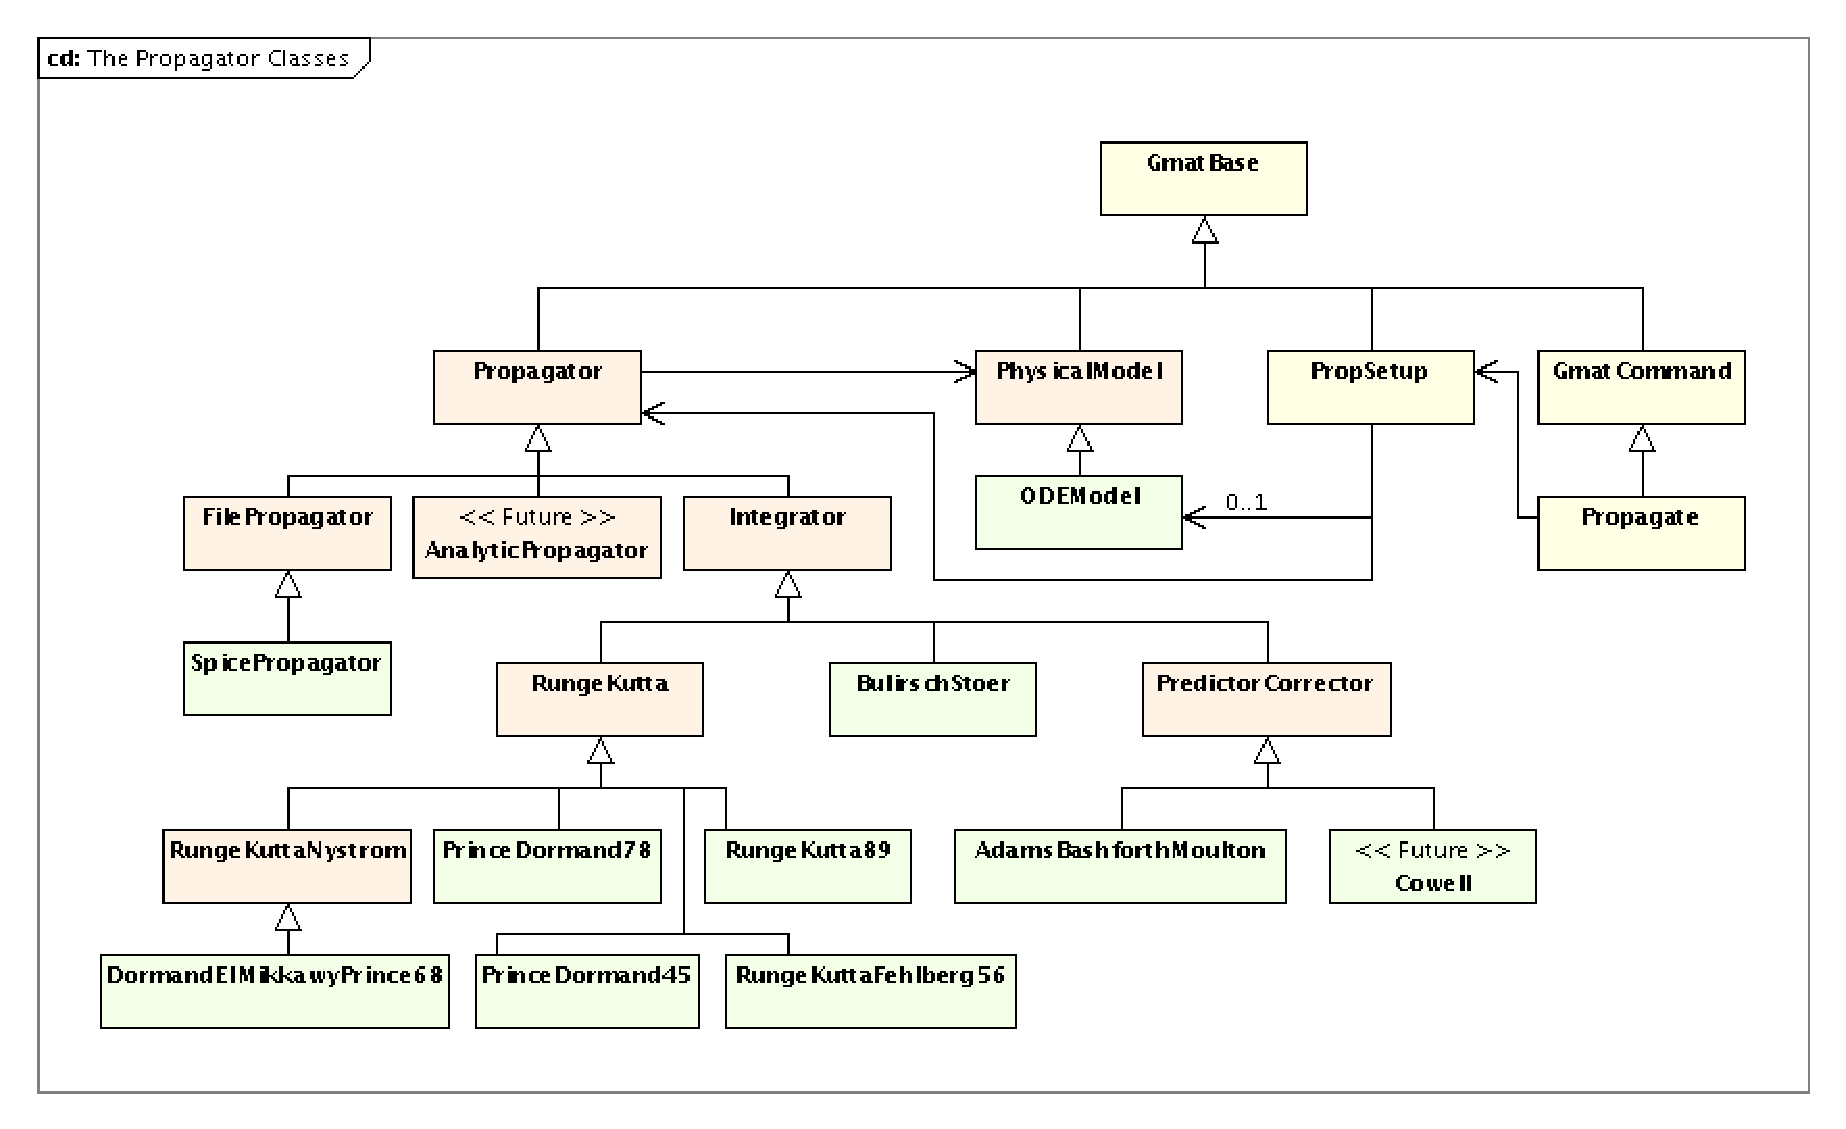
\includegraphics[scale=0.5]{Images/ThePropagatorClasses.eps}
\caption[Classes Used to Propagate State Data]{\label{figure:PropagatorClasses}Classes Used
to Propagate State Data.  Base classes are shown in orange.  Classes that instantiate the objects
used in numerical integration are in green.  Analytic propagation elements are in blue.  Classes
that are used to drive the propagation process, and other base level classes, are shown in yellow.}
\end{center}
\end{figure}

The numerical integration portion of the propagation system, shown in green in the figure, consists
of a differential equation model and numerical integrator paired to perform the precision
integration. The ODEModel class is a container class that accumulates all of the differential
equation data modeled in the mission, and reports the resulting changes in the elements of the
state vector. Details of the force model components of the differential equation model are described
in Chapter~\ref{chapter:ForceModel}.  Other differential equation models are described separately.

\section{The Propagator Base Class}

\subsection{Class Attributes}

\begin{itemize}
\item \textbf{PropVector *thePropVector}
\end{itemize}

\subsection{Class Methods}

\begin{itemize}
\item \textbf{bool Initialize()}
\end{itemize}

\section{Numerical Integration}


\subsection{\label{section:TheODEModel} The Derivative Models}

\begin{figure}[htb]
\begin{center}
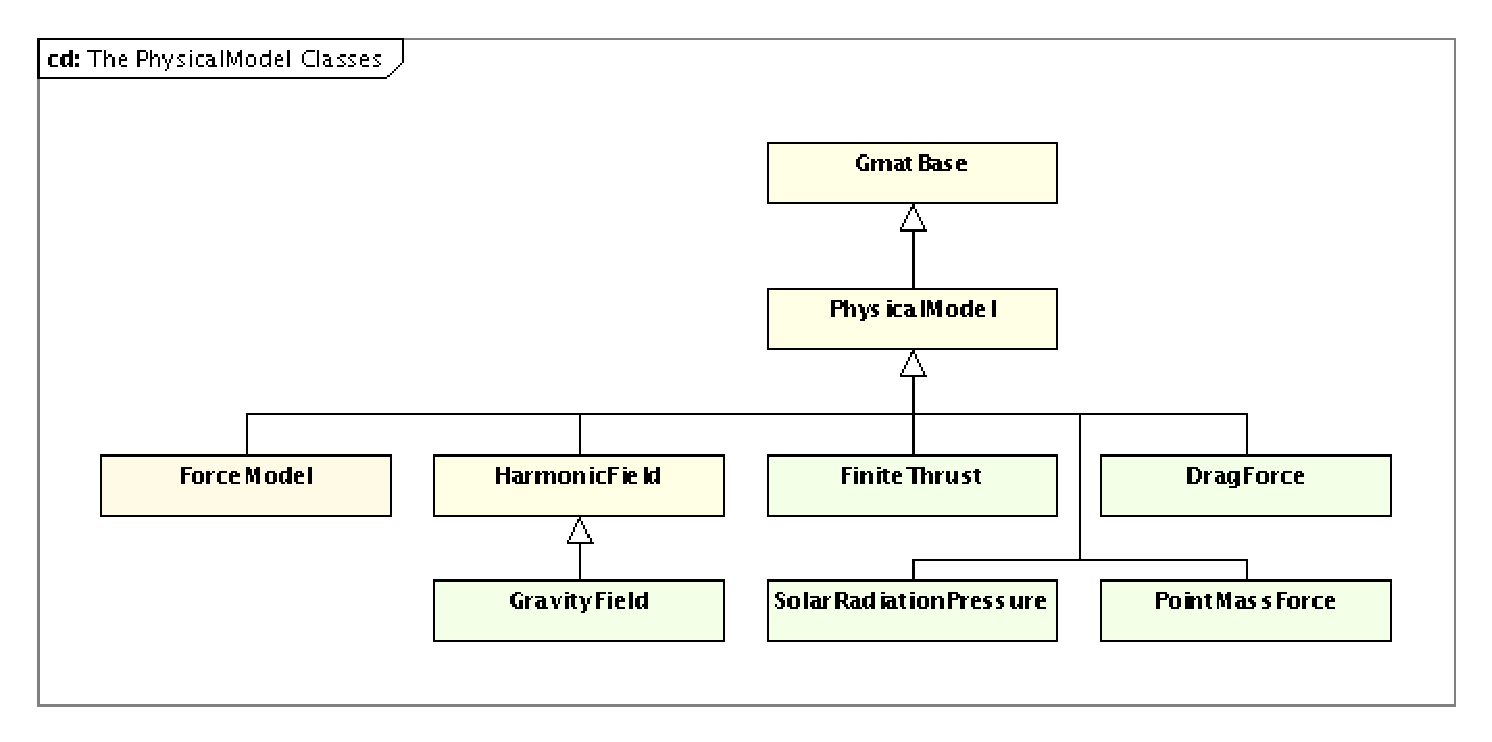
\includegraphics[scale=0.5]{Images/ThePhysicalModelClasses.eps}
\caption[The Derivative Model Classes]{\label{figure:PhysicalModelClasses}The Derivative Model
Classes.  This figure shows the classes used to provide derivative information to GMAT's
integrators.}
\end{center}
\end{figure}

\subsection{Initialization of the Derivative Model}


\begin{figure}[htb]
\begin{center}
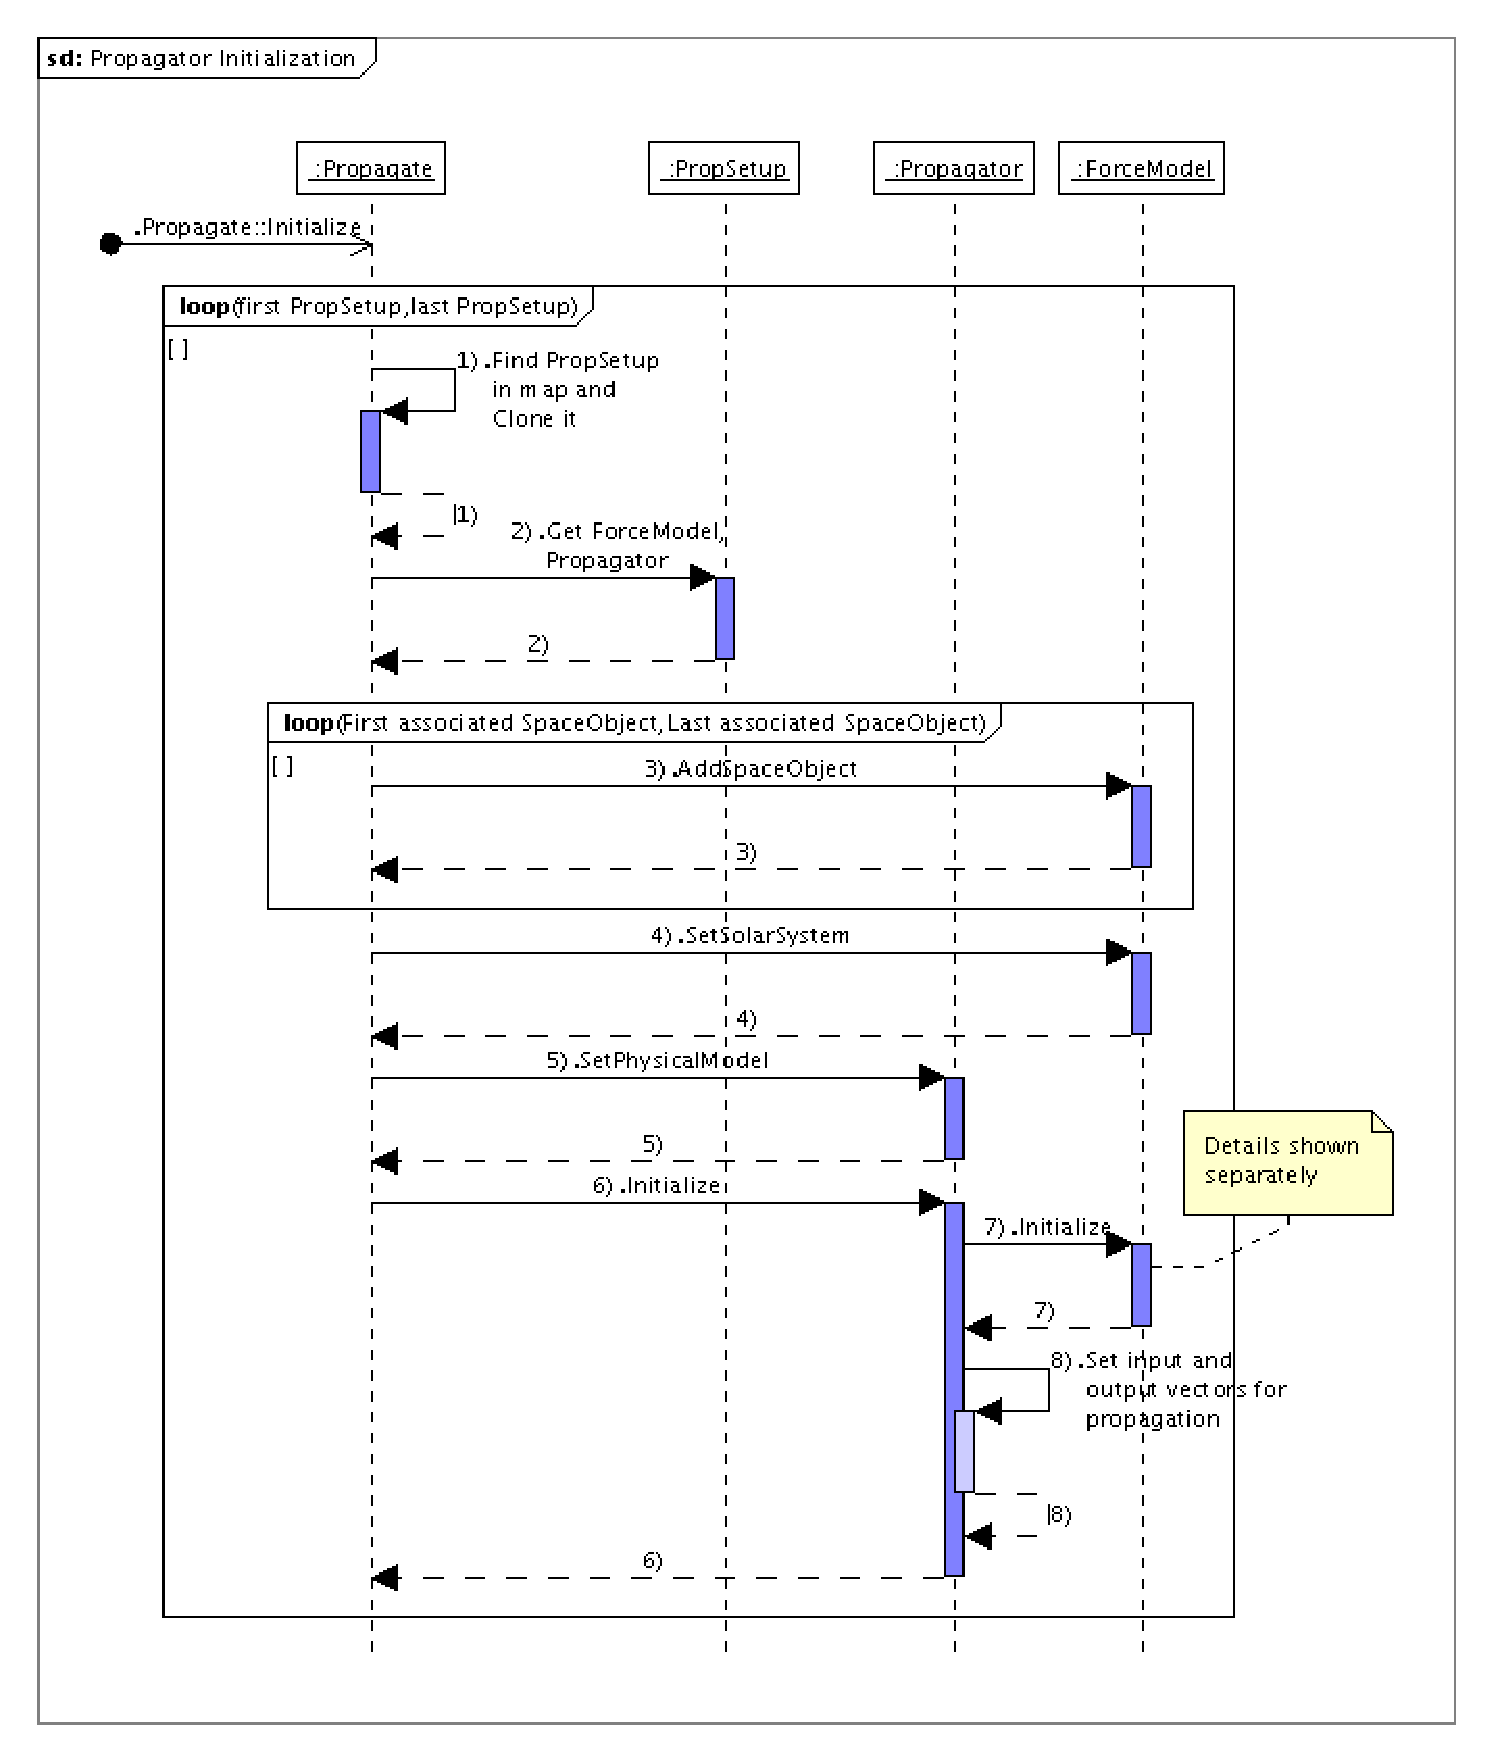
\includegraphics[scale=0.5]{Images/PropagatorInitialization.eps}
\caption[Propagator Initialization]{\label{figure:PropagatorInitialization}Propagator
Initialization.  This sequence diagram shows the process used to prepare a propagator for use in
the Mission Control Sequence.}
\end{center}
\end{figure}


\begin{figure}[htb]
\begin{center}
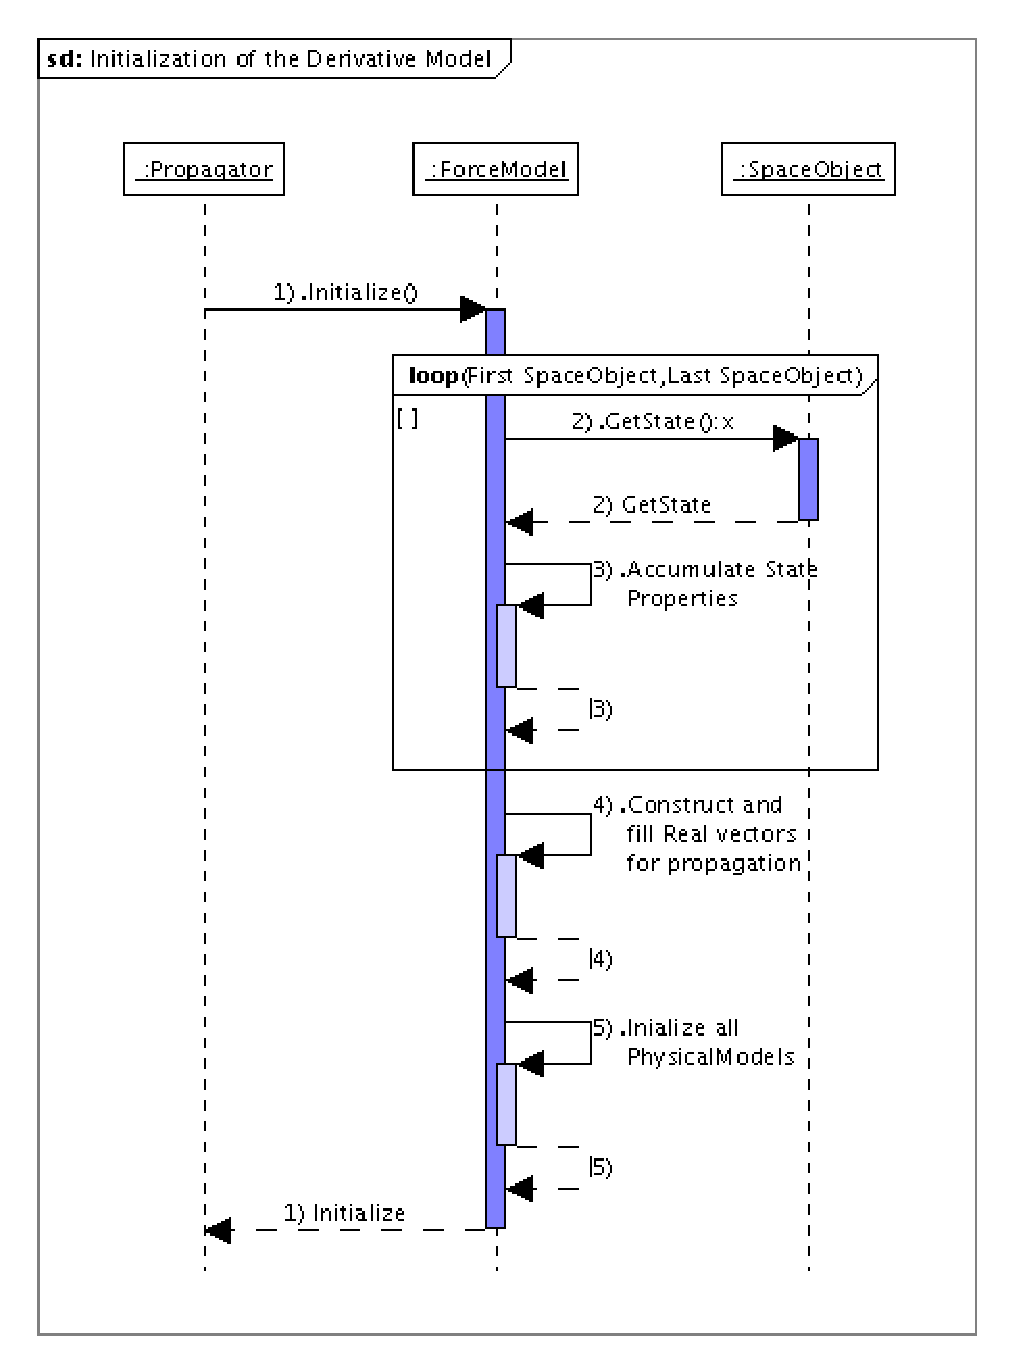
\includegraphics[scale=0.5]{Images/InitializationoftheDerivativeModel.eps}
\caption[Derivative Model Initialization]{\label{figure:DerivativeModelInitialization}Derivative
Model Initialization.  This sequence diagram shows the process used to build the data that is
numerically integrated during propagation.}
\end{center}
\end{figure}


\subsection{Finalizing Initialization: The PrepareToPropagate() Method}

\begin{figure}[htb]
\begin{center}
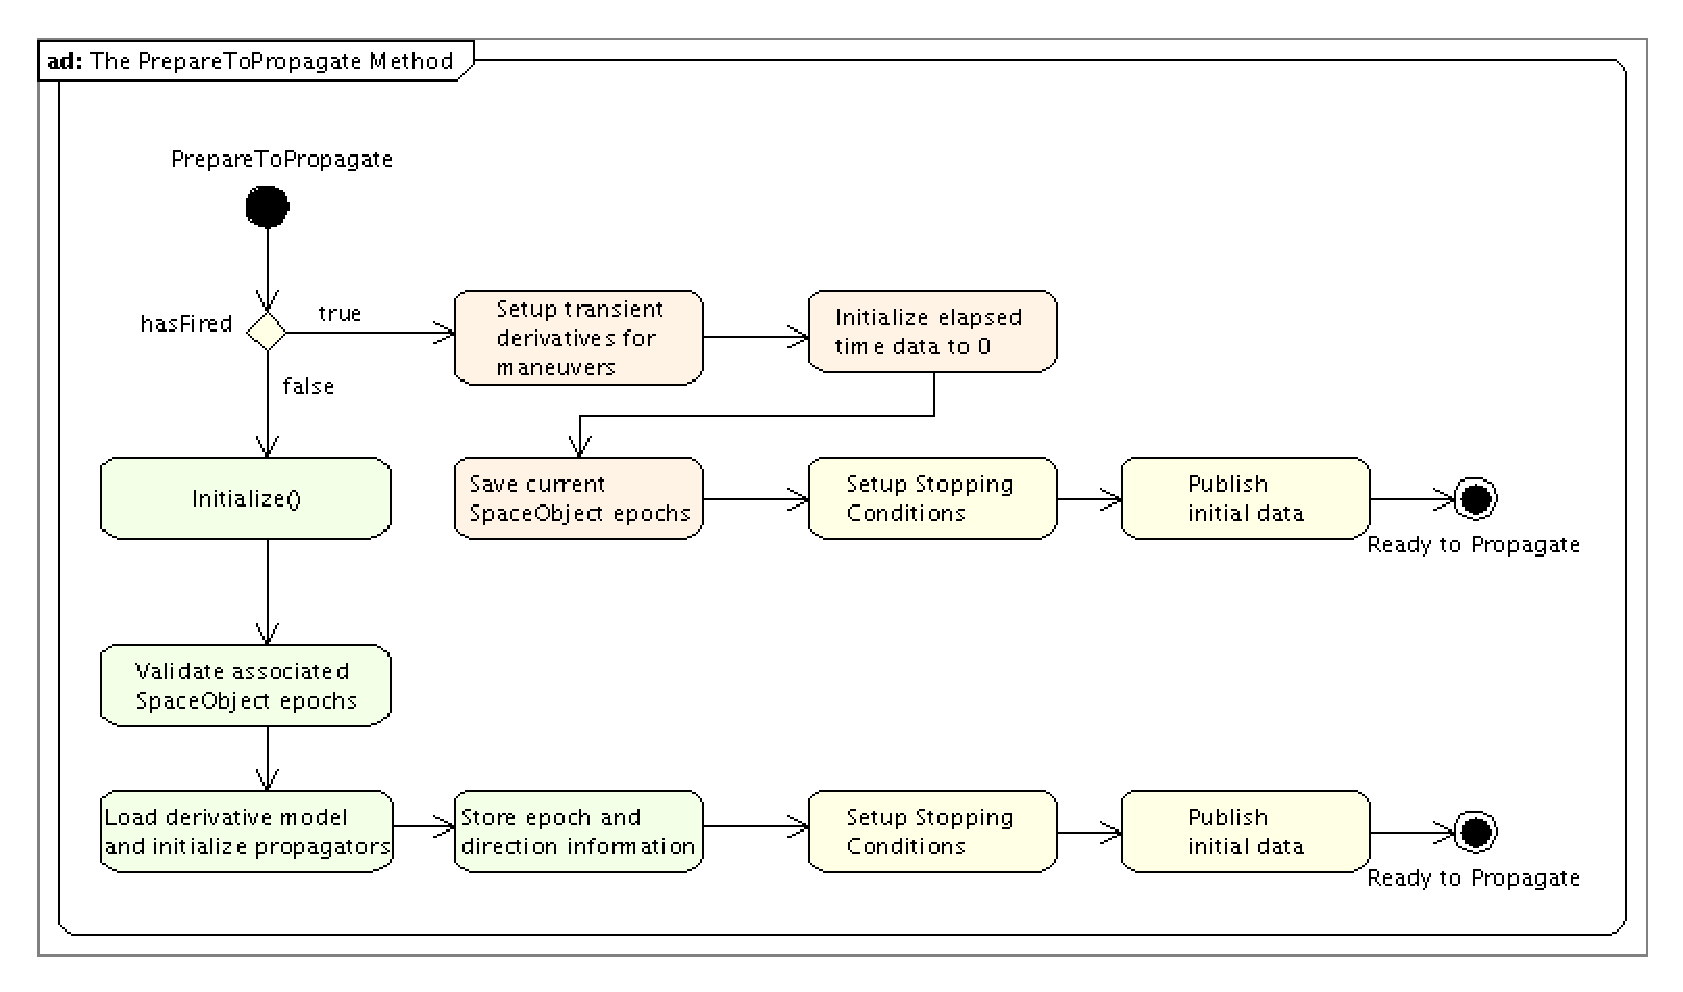
\includegraphics[scale=0.5]{Images/ThePrepareToPropagateMethod.eps}
\caption[Final Propagator Initialization:PrepareToPropagate())]
{\label{figure:PrepareToPropagate}Final Propagator Initialization:
PrepareToPropagate()}
\end{center}
\end{figure}


\subsection{Propagation}



\subsection{Completing Propagation}


\section{Analytic Propagation}

\section{File Based Propagation}

\section{Propagation Examples}

\subsection{\label{section:IntegratorExample}A Numerical Integration Example}

\subsection{\label{section:SpiceExample}A SPICE File Propagation Example}

\subsection{\label{section:MixedModePropagation}A Mixed Mode Example}

\index{Propagators}
\chapter{Calculation Parameters}
\label{Ch:CalcParameters}

GMAT's Central Body (Cb)\index{Cb} and Coordinate System
(CS)\index{CS} dependent parameters were tested to verify that the
internal calculations were correct. In order to minimize the effects
of other forces/elements, the two-body cases from the Propagators
section were used, with some modification, to test both the central
body and coordinate system parameters. The only changes to the two
body cases were in the report output intervals and report output
parameters. Data was outputted in ten minute intervals. The
ISS\index{ISS} two-body case was used for the Earth case and each
planets respective two-body case was used for the non-Earth cases.

\section{Initial Orbit State Conditions}
The ISS\index{ISS}, GEO\index{GEO}, Mars1, Mercury1, Moon, Neptune1,
Pluto1, Saturn1, Uranus1 and Venus1 two-body case's initial orbit
parameters were used from the Propagation\index{Propagation} section
(Chapter~\ref{Ch:Propagators}) for the test cases in this section.

Refer to Appendix ~\ref{Sec:initCondsProp} Tables~\ref{Table:
InitStateISS}-~\ref{Table: InitStateVenus} for a listing of all
Propagator initial orbit states used for the Calculation Parameter
test cases.

\section{Central Body Dependent Parameters}
\subsection{Naming Convention}
\label{nameConvCb}
This section describes the naming convention for central body
dependent parameter scripts and output reports. The naming
convention consists of a case sensitive ordered series of option
strings, separated by underscores (\_ ). Currently, options are
allowed for the following fields, and will be present in the file
name:
\begin{enumerate}
  \item \emph{tool} - The tool used to generate the test case.
  \item \emph{traj} - The trajectory to use.  This includes initial conditions, physical parameters, and time
  step.
\end{enumerate}

CbParams precedes the \emph{tool} field and 2Body follows the
\emph{traj} field. The central body used can be determined based on
the \emph{traj} field. The final Cb file format is as followed:\\
CbParams\_\emph{tool}\_\emph{traj}\_2Body.report\\

The \emph{tool} field should always be the first option field. Each
field has a finite list of options, as follows (future options
should be added to this list):
\begin{enumerate}
  \item \emph{tool}\\
  \begin{tabular}{ll}
    STK  & - Satellite Toolkit HPOP or Astrogator\\
    FF   & - FreeFlyer\\
    GMAT & - General Mission Analysis Tool\\
  \end{tabular}

  \item \emph{traj}\\
  \begin{tabular}{ll}
    ISS & - leo orbit\\
    Mars1 & - eccentric low orbit\\
    Mercury1 & - eccentric low orbit\\
    Moon & - eccentric low orbit\\
    Pluto1 & - eccentric low orbit\\
    Venus1 & - eccentric low orbit\\
  \end{tabular}

NOTE:  Some test cases contain \emph{traj} variations. In this case
\emph{traj} precedes the modification. For example, if an ISS
trajectory is needed with a different Cd, \emph{traj} could be
ISSdiffCd1.

\end{enumerate}


\subsection{Comparison Script Information}
Comparison\_Tool1\_Tool2\_Cb.m is the script used to perform the
coordinate system comparisons needed for the Acceptance Test Plan.
Many elements of this script were extracted from the
Comparison\_Tool1\_Tool2\_CS.m script.

Comparison\_Tool1\_Tool2\_Cb.m was designed to allow the user to
select two programs to compare to one another. The comparison
involves taking the difference of the variables listed in the
Acceptance Test Plan Overview Chapter-$>$Testing
Methodology-$>$Calculation Parameters section.

Refer to Appendix~\ref{Ch:CompScripts} for more details on this
script and others used in the Acceptance Test Plan document.

\subsection{Test Case Results}
The following results are for the Central Body-Calculation Parameter
section. The current GMAT Build is compared to STK\index{STK} and
FreeFlyer\index{FreeFlyer} for this section.

FF-STK comparison results presented in Tables~\ref{Table: FF-STK CB
Parameters Set 1}-~\ref{Table: FF-STK CB Parameters Set 5} are used
as a way to determine if the GMAT comparison values are acceptable.
If GMAT comparison data is within the same order of magnitude as the
FF-STK comparison data, that is acceptable. A more detailed
acceptance metric/matrix will be developed at a later date.

\begin{table}[htbp!]
\centering
\caption{ WinGMAT/STK Central Body Dependent Parameter Differences (1)}
      \begin{tabular}{lccccc}
      \hline\hline
          Test Case & Altitude (m) & Eccentricity & M. Anomaly (deg) & M. Motion (rad/sec) & Period (sec) \\
         \hline
         %---New Row---%
         GEO-2Body & 1.89175e-006 & 1.71688e-014 & 1.90373e-005 & 3.0114e-015 & 3.55067e-009 \\
         %---New Row---%
         Hyperbolic-2Body & 0.00422986 & 1.98064e-013 & 351.401 & 0.000223215 & N/A \\
         %---New Row---%
         ISS-2Body & 0.00543367 & 5.95719e-014 & 5.82162e-010 & 4.99015e-015 & 2.5193e-010 \\
         %---New Row---%
         Mars1-2Body & 0.0144309 & 9.74698e-011 & 7.84791e-007 & 1.62511e-013 & 2.29212e-006 \\
         %---New Row---%
         Mercury1-2Body & 0.00224375 & 2.36836e-011 & 1.7241e-007 & 5.54375e-014 & 7.66082e-007 \\
         %---New Row---%
         Moon-2Body & 2.60019e-005 & 1.24706e-013 & 2.88698e-009 & 3.85868e-016 & 7.42875e-009 \\
         %---New Row---%
         Neptune1-2Body & 0.129938 & 1.31684e-010 & 6.04911e-007 & 1.00481e-013 & 4.02816e-006 \\
         %---New Row---%
         Pluto1-2Body & 0.19231 & 1.83823e-009 & 2.95607e-005 & 3.82792e-012 & 0.000141823 \\
         %---New Row---%
         Saturn1-2Body & 0.752271 & 1.05362e-011 & 6.3449e-008 & 1.11997e-014 & 1.04643e-006 \\
         %---New Row---%
         Uranus1-2Body & 0.216614 & 5.31596e-011 & 6.35362e-007 & 8.48005e-014 & 8.31598e-006 \\
         %---New Row---%
         Venus1-2Body & 0.000632367 & 1.26323e-011 & 2.13253e-008 & 1.53591e-014 & 1.51652e-007 \\
      \hline\hline
      \label{Table: WinGMAT-STK CB Parameters Set 1} 
\end{tabular}
\end{table}
\index{STK}
\begin{table}[htbp!]
\centering
\caption{ WinGMAT/STK Central Body Dependent Parameter Differences (2)}
      \begin{tabular}{lccc}
      \hline\hline
          Test Case & Semi-major Axis (m) & True Anomaly (deg) & Semilatus Rectum(m) \\
         \hline
         %---New Row---%
         GEO-2Body & 1.16415e-006 & 1.90373e-005 & 7.42148e-007 \\
         %---New Row---%
         Hyperbolic-2Body & 1.648e-006 & 7.53175e-012 & 1.32495e-005 \\
         %---New Row---%
         ISS-2Body & 2.06455e-007 & 5.78609e-010 & 1.71894e-007 \\
         %---New Row---%
         Mars1-2Body & 0.000741843 & 1.15747e-006 & 0.000794765 \\
         %---New Row---%
         Mercury1-2Body & 0.000199977 & 2.61636e-007 & 0.000175894 \\
         %---New Row---%
         Moon-2Body & 1.10276e-006 & 4.32073e-009 & 1.07548e-006 \\
         %---New Row---%
         Neptune1-2Body & 0.00597339 & 9.2047e-007 & 0.00497125 \\
         %---New Row---%
         Pluto1-2Body & 0.0111278 & 4.499e-005 & 0.0106515 \\
         %---New Row---%
         Saturn1-2Body & 0.00241793 & 9.55595e-008 & 0.00235179 \\
         %---New Row---%
         Uranus1-2Body & 0.0100126 & 9.19017e-007 & 0.00930848 \\
         %---New Row---%
         Venus1-2Body & 0.000101745 & 3.07957e-008 & 0.00013864 \\
      \hline\hline
      \label{Table: WinGMAT-STK CB Parameters Set 2} 
\end{tabular}
\end{table}
\index{STK}
\begin{table}[htbp!]
\centering
\caption{ WinGMAT/STK Central Body Dependent Parameter Differences (3)}
      \begin{tabular}{lcccc}
      \hline\hline
          Test Case & Apoapsis Rad. (m) & Periapsis Rad. (m) & Apo. Vel. ($m/sec$) & Per. Vel. ($m/sec$) \\
         \hline
         %---New Row---%
         GEO-2Body & 1.23691e-006 & 1.28057e-006 & 8.21565e-011 & 1.03029e-010 \\
         %---New Row---%
         Hyperbolic-2Body & N/A & 4.5402e-006 & N/A & 1.87583e-009 \\
         %---New Row---%
         ISS-2Body & 5.26597e-007 & 3.39242e-007 & 4.40536e-010 & 3.47278e-010 \\
         %---New Row---%
         Mars1-2Body & 0.000683647 & 0.000800039 & 2.75849e-007 & 4.86309e-007 \\
         %---New Row---%
         Mercury1-2Body & 0.000280259 & 0.000125894 & 7.84977e-008 & 7.33316e-008 \\
         %---New Row---%
         Moon-2Body & 1.18234e-006 & 1.12323e-006 & 2.56017e-010 & 5.06262e-010 \\
         %---New Row---%
         Neptune1-2Body & 0.0107941 & 0.00538058 & 2.2861e-006 & 2.18703e-006 \\
         %---New Row---%
         Pluto1-2Body & 0.0145814 & 0.00998796 & 2.30184e-006 & 3.55073e-006 \\
         %---New Row---%
         Saturn1-2Body & 0.002828 & 0.00203526 & 2.94648e-007 & 5.08262e-007 \\
         %---New Row---%
         Uranus1-2Body & 0.0133233 & 0.00759641 & 1.41239e-006 & 1.43534e-006 \\
         %---New Row---%
         Venus1-2Body & 0.000149412 & 0.000183741 & 6.66214e-008 & 1.50022e-007 \\
      \hline\hline
      \label{Table: WinGMAT-STK CB Parameters Set 3} 
\end{tabular}
\end{table}
\index{STK}
\begin{table}[htbp!]
\centering
\caption{ WinGMAT/STK Central Body Dependent Parameter Differences (4)}
      \begin{tabular}{lccccc}
      \hline\hline
          Test Case & C3-Energy ($m^2/sec^2$) & Latitude (deg) & Longitude (deg) & MHA (deg) & LST (deg) \\
         \hline
         %---New Row---%
         GEO-2Body & 2.6823e-007 & 3.24498e-008 & 3.14812e-007 & 0.00196854 & 0.00196864 \\
         %---New Row---%
         Hyperbolic-2Body & 1.64846e-006 & 5.65537e-008 & 1.35016e-007 & 0.00196849 & 0.00196858 \\
         %---New Row---%
         ISS-2Body & 1.74794e-006 & 1.07149e-007 & 1.3276e-007 & 0.00196849 & 0.0019686 \\
         %---New Row---%
         Mars1-2Body & 0.00149955 & 5.58338e-007 & 9.73051e-007 & N/A & N/A \\
         %---New Row---%
         Mercury1-2Body & 0.000332532 & 1.88133e-007 & 2.69651e-007 & N/A & N/A \\
         %---New Row---%
         Moon-2Body & 8.62199e-007 & 3.26031e-009 & 1.41482e-007 & N/A & N/A \\
         %---New Row---%
         Neptune1-2Body & 0.0333365 & 7.39515e-007 & 1.15656e-006 & N/A & N/A \\
         %---New Row---%
         Pluto1-2Body & 0.00339014 & 3.20069e-005 & 7.44124e-005 & N/A & N/A \\
         %---New Row---%
         Saturn1-2Body & 0.014334 & 1.24281e-006 & 5.18835e-007 & N/A & N/A \\
         %---New Row---%
         Uranus1-2Body & 0.028651 & 9.64237e-007 & 2.34538e-006 & N/A & N/A \\
         %---New Row---%
         Venus1-2Body & 0.000500677 & 2.22686e-008 & 3.82501e-008 & N/A & N/A \\
      \hline\hline
      \label{Table: WinGMAT-STK CB Parameters Set 4} 
\end{tabular}
\end{table}
\index{STK}
\begin{table}[htbp!]
\centering
\caption{ WinGMAT/STK Central Body Dependent Parameter Differences (5)}
      \begin{tabular}{lccc}
      \hline\hline
          Test Case & Beta Angle (deg) & (RxV)-Mag ($m^2/sec$) & R-Mag (m) \\
         \hline
         %---New Row---%
         GEO-2Body & 45.7421 & 0.00180444 & 1.88447e-006 \\
         %---New Row---%
         Hyperbolic-2Body & 130.969 & 0.025655 & 1.35624e-005 \\
         %---New Row---%
         ISS-2Body & 98.3615 & 0.000749424 & 4.62933e-007 \\
         %---New Row---%
         Mars1-2Body & 70.1724 & 1.23719 & 0.0126011 \\
         %---New Row---%
         Mercury1-2Body & 173.794 & 0.220796 & 0.00224375 \\
         %---New Row---%
         Moon-2Body & 34.7765 & 0.00081809 & 2.6002e-005 \\
         %---New Row---%
         Neptune1-2Body & 122.85 & 35.4559 & 0.0763421 \\
         %---New Row---%
         Pluto1-2Body & 56.4158 & 4.01956 & 0.19231 \\
         %---New Row---%
         Saturn1-2Body & 99.1135 & 26.1241 & 0.0181717 \\
         %---New Row---%
         Uranus1-2Body & 150.273 & 53.902 & 0.101524 \\
         %---New Row---%
         Venus1-2Body & 31.881 & 0.447268 & 0.000632365 \\
      \hline\hline
      \label{Table: WinGMAT-STK CB Parameters Set 5} 
\end{tabular}
\end{table}
\index{STK}
\clearpage

\begin{table}[htbp!]
\centering
\caption{ FF/WinGMAT Central Body Dependent Parameter Differences (1)}
      \begin{tabular}{lccccc}
      \hline\hline
          Test Case & Altitude (m) & Eccentricity & M. Anomaly (deg) & M. Motion (rad/sec) & Period (sec) \\
         \hline
         %---New Row---%
         GEO-2Body & 8.20728e-006 & 1.93962e-010 & 6.42153e-006 & 5.69653e-016 & 7.75617e-009 \\
         %---New Row---%
         ISS-2Body & 0.433346 & 6.39335e-012 & 1.714e-009 & 4.2466e-015 & 7.69433e-010 \\
      \hline\hline
      \label{Table: FF-WinGMAT CB Parameters Set 1} 
\end{tabular}
\end{table}
\index{FreeFlyer}
\begin{table}[htbp!]
\centering
\caption{ FF/WinGMAT Central Body Dependent Parameter Differences (2)}
      \begin{tabular}{lccc}
      \hline\hline
          Test Case & Semi-major Axis (m) & True Anomaly (deg) & Semilatus Rectum(m) \\
         \hline
         %---New Row---%
         GEO-2Body & 2.23372e-006 & 6.4215e-006 & 2.4811e-006 \\
         %---New Row---%
         ISS-2Body & 4.09273e-007 & 1.86708e-009 & 1.7917e-007 \\
      \hline\hline
      \label{Table: FF-WinGMAT CB Parameters Set 2} 
\end{tabular}
\end{table}
\index{FreeFlyer}
\begin{table}[htbp!]
\centering
\caption{ FF/WinGMAT Central Body Dependent Parameter Differences (3)}
      \begin{tabular}{lcccc}
      \hline\hline
          Test Case & Apoapsis Rad. (m) & Periapsis Rad. (m) & Apo. Vel. ($m/sec$) & Per. Vel. ($m/sec$) \\
         \hline
         %---New Row---%
         GEO-2Body & 2.72848e-006 & 3.00497e-006 & 2.39764e-008 & 2.39013e-008 \\
         %---New Row---%
         ISS-2Body & 3.98359e-007 & 6.89397e-007 & 2.91838e-008 & 2.88605e-008 \\
      \hline\hline
      \label{Table: FF-WinGMAT CB Parameters Set 3} 
\end{tabular}
\end{table}
\index{FreeFlyer}
\begin{table}[htbp!]
\centering
\caption{ FF/WinGMAT Central Body Dependent Parameter Differences (4)}
      \begin{tabular}{lccccc}
      \hline\hline
          Test Case & C3-Energy ($m^2/sec^2$) & Latitude (deg) & Longitude (deg) & MHA (deg) & LST (deg) \\
         \hline
         %---New Row---%
         GEO-2Body & 0.00014728 & 5.40781e-008 & 0 & 0.00300898 & 0.00300919 \\
         %---New Row---%
         ISS-2Body & 0.000444231 & 6.02545e-006 & 5.81869e-007 & 0.00300898 & 0.00300919 \\
      \hline\hline
      \label{Table: FF-WinGMAT CB Parameters Set 4} 
\end{tabular}
\end{table}
\index{FreeFlyer}
\begin{table}[htbp!]
\centering
\caption{ FF/WinGMAT Central Body Dependent Parameter Differences (5)}
      \begin{tabular}{lccc}
      \hline\hline
          Test Case & Beta Angle (deg) & (RxV)-Mag ($m^2/sec$) & R-Mag (m) \\
         \hline
         %---New Row---%
         GEO-2Body & 45.7413 & 0.00429281 & 3.27418e-006 \\
         %---New Row---%
         ISS-2Body & 98.3649 & 0.00164437 & 1.18325e-006 \\
      \hline\hline
      \label{Table: FF-WinGMAT CB Parameters Set 5} 
\end{tabular}
\end{table}
\index{FreeFlyer}
\clearpage

\begin{table}[htbp!]
\centering
\caption{ FF/STK Central Body Dependent Parameter Differences (1)}
      \begin{tabular}{lccccc}
      \hline\hline
          Test Case & Altitude (m) & Eccentricity & M. Anomaly (deg) & M. Motion (rad/sec) & Period (sec) \\
         \hline
         %---New Row---%
         GEO-2Body & 8.04721e-006 & 1.9396e-010 & 1.76421e-005 & 2.44679e-015 & 6.4756e-009 \\
         %---New Row---%
         ISS-2Body & 0.427915 & 6.34e-012 & 1.73014e-009 & 9.18666e-015 & 8.14907e-010 \\
      \hline\hline
      \label{Table: FF-STK CB Parameters Set 1} 
\end{tabular}
\end{table}
\index{STK}\index{FreeFlyer}
\begin{table}[htbp!]
\centering
\caption{ FF/STK Central Body Dependent Parameter Differences (2)}
      \begin{tabular}{lccc}
      \hline\hline
          Test Case & Semi-major Axis (m) & True Anomaly (deg) & Semilatus Rectum(m) \\
         \hline
         %---New Row---%
         GEO-2Body & 2.08092e-006 & 1.76414e-005 & 1.92085e-006 \\
         %---New Row---%
         ISS-2Body & 4.47471e-007 & 1.67717e-009 & 1.56433e-007 \\
      \hline\hline
      \label{Table: FF-STK CB Parameters Set 2} 
\end{tabular}
\end{table}
\index{STK}\index{FreeFlyer}
\begin{table}[htbp!]
\centering
\caption{ FF/STK Central Body Dependent Parameter Differences (3)}
      \begin{tabular}{lcccc}
      \hline\hline
          Test Case & Apoapsis Rad. (m) & Periapsis Rad. (m) & Apo. Vel. ($m/sec$) & Per. Vel. ($m/sec$) \\
         \hline
         %---New Row---%
         GEO-2Body & 2.72848e-006 & 2.03727e-006 & 2.38942e-008 & 2.38796e-008 \\
         %---New Row---%
         ISS-2Body & 5.23869e-007 & 6.23913e-007 & 2.87432e-008 & 2.88605e-008 \\
      \hline\hline
      \label{Table: FF-STK CB Parameters Set 3} 
\end{tabular}
\end{table}
\index{STK}\index{FreeFlyer}
\begin{table}[htbp!]
\centering
\caption{ FF/STK Central Body Dependent Parameter Differences (4)}
      \begin{tabular}{lccccc}
      \hline\hline
          Test Case & C3-Energy ($m^2/sec^2$) & Latitude (deg) & Longitude (deg) & MHA (deg) & LST (deg) \\
         \hline
         %---New Row---%
         GEO-2Body & 0.000147141 & 3.06691e-008 & 0 & 0.00497708 & 0.00497715 \\
         %---New Row---%
         ISS-2Body & 0.000442895 & 5.92635e-006 & 6.1431e-007 & 0.00497708 & 0.00497716 \\
      \hline\hline
      \label{Table: FF-STK CB Parameters Set 4} 
\end{tabular}
\end{table}
\index{STK}\index{FreeFlyer}
\begin{table}[htbp!]
\centering
\caption{ FF/STK Central Body Dependent Parameter Differences (5)}
      \begin{tabular}{lccc}
      \hline\hline
          Test Case & Beta Angle (deg) & (RxV)-Mag ($m^2/sec$) & R-Mag (m) \\
         \hline
         %---New Row---%
         GEO-2Body & 0.000773444 & 0.00355067 & 4.05998e-006 \\
         %---New Row---%
         ISS-2Body & 0.00344889 & 0.00178261 & 1.01772e-006 \\
      \hline\hline
      \label{Table: FF-STK CB Parameters Set 5} 
\end{tabular}
\end{table}
\index{STK}\index{FreeFlyer}
\clearpage

\subsection{Win/Mac GMAT Comparison}
\begin{table}[htbp!]
\centering
\caption{ WinGMAT/MacGMAT Central Body Dependent Parameter Differences (1)}
      \begin{tabular}{lccccc}
      \hline\hline
          Test Case & Altitude (m) & Eccentricity & M. Anomaly (deg) & M. Motion (rad/sec) & Period (sec) \\
         \hline
         %---New Row---%
         GEO-2Body & 2.452e-006 & 1.74542e-014 & 8.52452e-006 & 6.93889e-018 & 8.22183e-009 \\
         %---New Row---%
         Hyperbolic-2Body & 5.23869e-007 & 9.99201e-015 & 0 & 1.0842e-018 & N/A \\
         %---New Row---%
         ISS-2Body & 4.58385e-007 & 3.9682e-014 & 1.38419e-009 & 8.39172e-017 & 4.02906e-010 \\
         %---New Row---%
         Mars1-2Body & 0.00342313 & 1.47847e-010 & 2.00985e-007 & 1.34903e-013 & 1.93017e-006 \\
         %---New Row---%
         Mercury1-2Body & 0.00505079 & 4.83717e-011 & 3.89952e-007 & 1.08871e-013 & 1.49741e-006 \\
         %---New Row---%
         Moon-2Body & 2.24818e-005 & 1.43691e-013 & 2.53274e-009 & 4.53522e-016 & 9.08949e-009 \\
         %---New Row---%
         Neptune1-2Body & 2.00089e-008 & 4.93383e-013 & 4.70095e-011 & 2.99186e-016 & 1.17889e-008 \\
         %---New Row---%
         Pluto1-2Body & 0.0110934 & 9.63307e-010 & 1.50655e-006 & 1.2462e-012 & 4.61344e-005 \\
         %---New Row---%
         Saturn1-2Body & 5.09317e-008 & 5.10703e-015 & 1.19371e-012 & 2.81893e-018 & 2.40107e-010 \\
         %---New Row---%
         Uranus1-2Body & 3.09228e-008 & 1.8624e-014 & 7.95808e-012 & 1.24141e-017 & 1.22236e-009 \\
         %---New Row---%
         Venus1-2Body & 0.00131446 & 1.40132e-011 & 4.55151e-008 & 2.2602e-014 & 2.34479e-007 \\
      \hline\hline
      \label{Table: WinGMAT-MacGMAT CB Parameters Set 1} 
\end{tabular}
\end{table}

\begin{table}[htbp!]
\centering
\caption{ WinGMAT/MacGMAT Central Body Dependent Parameter Differences (2)}
      \begin{tabular}{lccc}
      \hline\hline
          Test Case & Semi-major Axis (m) & True Anomaly (deg) & Semilatus Rectum(m) \\
         \hline
         %---New Row---%
         GEO-2Body & 2.67755e-006 & 8.52451e-006 & 2.67755e-006 \\
         %---New Row---%
         Hyperbolic-2Body & 6.91216e-008 & 5.11591e-013 & 3.27418e-007 \\
         %---New Row---%
         ISS-2Body & 3.29237e-007 & 1.38273e-009 & 3.28328e-007 \\
         %---New Row---%
         Mars1-2Body & 0.000624696 & 3.06826e-007 & 0.000545762 \\
         %---New Row---%
         Mercury1-2Body & 0.000390883 & 5.87062e-007 & 0.000336432 \\
         %---New Row---%
         Moon-2Body & 1.35014e-006 & 3.8051e-009 & 1.19917e-006 \\
         %---New Row---%
         Neptune1-2Body & 1.74914e-005 & 3.54987e-011 & 2.07729e-005 \\
         %---New Row---%
         Pluto1-2Body & 0.00361984 & 2.21937e-006 & 0.00371269 \\
         %---New Row---%
         Saturn1-2Body & 5.38421e-007 & 1.3074e-012 & 4.80213e-007 \\
         %---New Row---%
         Uranus1-2Body & 1.46974e-006 & 7.53175e-012 & 1.36788e-006 \\
         %---New Row---%
         Venus1-2Body & 0.000157314 & 6.88501e-008 & 0.000105473 \\
      \hline\hline
      \label{Table: WinGMAT-MacGMAT CB Parameters Set 2} 
\end{tabular}
\end{table}

\begin{table}[htbp!]
\centering
\caption{ WinGMAT/MacGMAT Central Body Dependent Parameter Differences (3)}
      \begin{tabular}{lcccc}
      \hline\hline
          Test Case & Apoapsis Rad. (m) & Periapsis Rad. (m) & Apo. Vel. ($m/sec$) & Per. Vel. ($m/sec$) \\
         \hline
         %---New Row---%
         GEO-2Body & 2.78669e-006 & 2.91766e-006 & 1.22125e-010 & 1.15019e-010 \\
         %---New Row---%
         Hyperbolic-2Body & N/A & 1.89175e-007 & N/A & 7.81597e-011 \\
         %---New Row---%
         ISS-2Body & 3.21052e-007 & 5.7571e-007 & 2.98428e-010 & 4.69846e-010 \\
         %---New Row---%
         Mars1-2Body & 0.00139151 & 0.000626785 & 5.33045e-007 & 5.19715e-007 \\
         %---New Row---%
         Mercury1-2Body & 0.000578938 & 0.00021615 & 1.72014e-007 & 1.50894e-007 \\
         %---New Row---%
         Moon-2Body & 1.92404e-006 & 8.39918e-007 & 4.62075e-010 & 3.57048e-010 \\
         %---New Row---%
         Neptune1-2Body & 3.5041e-005 & 2.87691e-005 & 7.62945e-009 & 1.22924e-008 \\
         %---New Row---%
         Pluto1-2Body & 0.00374967 & 0.00349214 & 4.00636e-007 & 1.2944e-006 \\
         %---New Row---%
         Saturn1-2Body & 1.06229e-006 & 7.05768e-007 & 1.59872e-010 & 2.02505e-010 \\
         %---New Row---%
         Uranus1-2Body & 2.55386e-006 & 1.56433e-006 & 3.23297e-010 & 3.8014e-010 \\
         %---New Row---%
         Venus1-2Body & 0.000302634 & 6.57656e-005 & 1.25344e-007 & 5.78817e-008 \\
      \hline\hline
      \label{Table: WinGMAT-MacGMAT CB Parameters Set 3} 
\end{tabular}
\end{table}

\begin{table}[htbp!]
\centering
\caption{ WinGMAT/MacGMAT Central Body Dependent Parameter Differences (4)}
      \begin{tabular}{lccccc}
      \hline\hline
          Test Case & C3-Energy ($m^2/sec^2$) & Latitude (deg) & Longitude (deg) & MHA (deg) & LST (deg) \\
         \hline
         %---New Row---%
         GEO-2Body & 6.00409e-007 & 5.68504e-014 & 3.10763e-010 & 1.16529e-010 & 3.10706e-010 \\
         %---New Row---%
         Hyperbolic-2Body & 7.10543e-008 & 6.03961e-014 & 2.24389e-010 & 1.16529e-010 & 2.24304e-010 \\
         %---New Row---%
         ISS-2Body & 2.8848e-006 & 5.10916e-011 & 2.10321e-010 & 1.16529e-010 & 2.10321e-010 \\
         %---New Row---%
         Mars1-2Body & 0.00126275 & 1.58843e-007 & 3.08052e-007 & N/A & N/A \\
         %---New Row---%
         Mercury1-2Body & 0.00064998 & 4.31925e-007 & 6.27266e-007 & N/A & N/A \\
         %---New Row---%
         Moon-2Body & 1.05893e-006 & 2.93206e-009 & 4.7355e-009 & N/A & N/A \\
         %---New Row---%
         Neptune1-2Body & 9.75149e-005 & 6.39488e-014 & 2.08502e-010 & N/A & N/A \\
         %---New Row---%
         Pluto1-2Body & 0.0011028 & 1.59299e-006 & 3.42747e-006 & N/A & N/A \\
         %---New Row---%
         Saturn1-2Body & 3.18323e-006 & 6.39488e-014 & 4.16918e-010 & N/A & N/A \\
         %---New Row---%
         Uranus1-2Body & 4.20641e-006 & 6.03961e-014 & 2.08502e-010 & N/A & N/A \\
         %---New Row---%
         Venus1-2Body & 0.000774136 & 5.2415e-008 & 8.42126e-008 & N/A & N/A \\
      \hline\hline
      \label{Table: WinGMAT-MacGMAT CB Parameters Set 4} 
\end{tabular}
\end{table}

\begin{table}[htbp!]
\centering
\caption{ WinGMAT/MacGMAT Central Body Dependent Parameter Differences (5)}
      \begin{tabular}{lccc}
      \hline\hline
          Test Case & Beta Angle (deg) & (RxV)-Mag ($m^2/sec$) & R-Mag (m) \\
         \hline
         %---New Row---%
         GEO-2Body & 1.42109e-014 & 0.00410364 & 2.43745e-006 \\
         %---New Row---%
         Hyperbolic-2Body & 7.10543e-014 & 0.000640284 & 4.07454e-007 \\
         %---New Row---%
         ISS-2Body & 5.96856e-013 & 0.00125874 & 4.65661e-007 \\
         %---New Row---%
         Mars1-2Body & 2.6164e-009 & 0.849539 & 0.0034188 \\
         %---New Row---%
         Mercury1-2Body & 1.88567e-009 & 0.422386 & 0.00505079 \\
         %---New Row---%
         Moon-2Body & 6.94911e-012 & 0.000856744 & 2.24832e-005 \\
         %---New Row---%
         Neptune1-2Body & 1.7053e-013 & 0.14808 & 1.45519e-008 \\
         %---New Row---%
         Pluto1-2Body & 2.51034e-008 & 1.40107 & 0.0110934 \\
         %---New Row---%
         Saturn1-2Body & 4.26326e-014 & 0.0060536 & 1.45519e-008 \\
         %---New Row---%
         Uranus1-2Body & 1.84741e-013 & 0.00791624 & 1.45519e-008 \\
         %---New Row---%
         Venus1-2Body & 1.98796e-010 & 0.34034 & 0.00131445 \\
      \hline\hline
      \label{Table: WinGMAT-MacGMAT CB Parameters Set 5} 
\end{tabular}
\end{table}

\clearpage

\subsection{Win/Linux GMAT Comparison}
\begin{table}[htbp!]
\centering
\caption{ WinGMAT/LinuxGMAT Central Body Dependent Parameter Differences (1)}
      \begin{tabular}{lccccc}
      \hline\hline
          Test Case & Altitude (m) & Eccentricity & M. Anomaly (deg) & M. Motion (rad/sec) & Period (sec) \\
         \hline
         %---New Row---%
         GEO-2Body & 1.45519e-008 & 1.05879e-022 & 1.02318e-012 & 0 & 0 \\
         %---New Row---%
         Hyperbolic-2Body & 1.16415e-007 & 8.88178e-016 & 0 & 1.0842e-019 & N/A \\
         %---New Row---%
         ISS-2Body & 1.13687e-010 & 1.0842e-018 & 1.13687e-013 & 1.0842e-018 & 1.81899e-012 \\
         %---New Row---%
         Mars1-2Body & 9.09495e-010 & 1.11022e-016 & 1.50635e-012 & 1.0842e-019 & 0 \\
         %---New Row---%
         Mercury1-2Body & 9.09495e-010 & 1.11022e-016 & 1.13687e-013 & 1.0842e-019 & 0 \\
         %---New Row---%
         Moon-2Body & 1.13687e-009 & 1.11022e-016 & 4.83169e-013 & 1.0842e-019 & 1.09139e-011 \\
         %---New Row---%
         Neptune1-2Body & 1.09139e-008 & 1.11022e-016 & 3.41061e-013 & 1.0842e-019 & 1.09139e-011 \\
         %---New Row---%
         Pluto1-2Body & 1.13687e-010 & 1.11022e-016 & 1.3074e-012 & 1.0842e-019 & 1.09139e-011 \\
         %---New Row---%
         Saturn1-2Body & 1.45519e-008 & 1.11022e-016 & 1.98952e-013 & 1.0842e-019 & 1.09139e-011 \\
         %---New Row---%
         Uranus1-2Body & 1.09139e-008 & 1.11022e-016 & 1.10845e-012 & 1.0842e-019 & 1.09139e-011 \\
         %---New Row---%
         Venus1-2Body & 1.02318e-009 & 1.11022e-016 & 5.55099e-013 & 1.0842e-019 & 1.81899e-012 \\
      \hline\hline
      \label{Table: WinGMAT-LinuxGMAT CB Parameters Set 1} 
\end{tabular}
\end{table}

\begin{table}[htbp!]
\centering
\caption{ WinGMAT/LinuxGMAT Central Body Dependent Parameter Differences (2)}
      \begin{tabular}{lccc}
      \hline\hline
          Test Case & Semi-major Axis (m) & True Anomaly (deg) & Semilatus Rectum(m) \\
         \hline
         %---New Row---%
         GEO-2Body & 1.45519e-008 & 9.09495e-013 & 1.45519e-008 \\
         %---New Row---%
         Hyperbolic-2Body & 1.09139e-008 & 1.13687e-013 & 7.27596e-009 \\
         %---New Row---%
         ISS-2Body & 1.81899e-009 & 1.13687e-013 & 1.81899e-009 \\
         %---New Row---%
         Mars1-2Body & 1.81899e-009 & 9.9476e-013 & 1.81899e-009 \\
         %---New Row---%
         Mercury1-2Body & 9.09495e-010 & 1.13687e-013 & 9.09495e-010 \\
         %---New Row---%
         Moon-2Body & 9.09495e-010 & 3.97904e-013 & 9.09495e-010 \\
         %---New Row---%
         Neptune1-2Body & 1.45519e-008 & 3.97904e-013 & 1.45519e-008 \\
         %---New Row---%
         Pluto1-2Body & 9.09495e-010 & 7.95808e-013 & 9.09495e-010 \\
         %---New Row---%
         Saturn1-2Body & 0 & 1.98952e-013 & 0 \\
         %---New Row---%
         Uranus1-2Body & 1.45519e-008 & 7.10543e-013 & 1.45519e-008 \\
         %---New Row---%
         Venus1-2Body & 1.81899e-009 & 8.4982e-013 & 1.81899e-009 \\
      \hline\hline
      \label{Table: WinGMAT-LinuxGMAT CB Parameters Set 2} 
\end{tabular}
\end{table}

\begin{table}[htbp!]
\centering
\caption{ WinGMAT/LinuxGMAT Central Body Dependent Parameter Differences (3)}
      \begin{tabular}{lcccc}
      \hline\hline
          Test Case & Apoapsis Rad. (m) & Periapsis Rad. (m) & Apo. Vel. ($m/sec$) & Per. Vel. ($m/sec$) \\
         \hline
         %---New Row---%
         GEO-2Body & 1.45519e-008 & 1.45519e-008 & 8.88178e-013 & 8.88178e-013 \\
         %---New Row---%
         Hyperbolic-2Body & N/A & 1.09139e-008 & N/A & 0 \\
         %---New Row---%
         ISS-2Body & 1.81899e-009 & 1.81899e-009 & 1.77636e-012 & 1.77636e-012 \\
         %---New Row---%
         Mars1-2Body & 1.81899e-009 & 9.09495e-010 & 8.88178e-013 & 8.88178e-013 \\
         %---New Row---%
         Mercury1-2Body & 1.81899e-009 & 9.09495e-010 & 8.88178e-013 & 8.88178e-013 \\
         %---New Row---%
         Moon-2Body & 9.09495e-010 & 9.09495e-010 & 8.88178e-013 & 8.88178e-013 \\
         %---New Row---%
         Neptune1-2Body & 1.45519e-008 & 1.09139e-008 & 1.06581e-011 & 1.06581e-011 \\
         %---New Row---%
         Pluto1-2Body & 9.09495e-010 & 9.09495e-010 & 0 & 0 \\
         %---New Row---%
         Saturn1-2Body & 0 & 1.45519e-008 & 1.06581e-011 & 1.06581e-011 \\
         %---New Row---%
         Uranus1-2Body & 1.45519e-008 & 1.45519e-008 & 0 & 1.06581e-011 \\
         %---New Row---%
         Venus1-2Body & 0 & 1.81899e-009 & 1.77636e-012 & 1.77636e-012 \\
      \hline\hline
      \label{Table: WinGMAT-LinuxGMAT CB Parameters Set 3} 
\end{tabular}
\end{table}

\begin{table}[htbp!]
\centering
\caption{ WinGMAT/LinuxGMAT Central Body Dependent Parameter Differences (4)}
      \begin{tabular}{lccccc}
      \hline\hline
          Test Case & C3-Energy ($m^2/sec^2$) & Latitude (deg) & Longitude (deg) & MHA (deg) & LST (deg) \\
         \hline
         %---New Row---%
         GEO-2Body & 0 & 1.04083e-017 & 0 & 1.13687e-013 & 1.13687e-013 \\
         %---New Row---%
         Hyperbolic-2Body & 1.06581e-008 & 1.06581e-014 & 1.13687e-013 & 1.13687e-013 & 1.13687e-013 \\
         %---New Row---%
         ISS-2Body & 1.42109e-008 & 1.42109e-014 & 1.13687e-013 & 1.13687e-013 & 1.13687e-013 \\
         %---New Row---%
         Mars1-2Body & 0 & 1.06581e-014 & 1.13687e-013 & N/A & N/A \\
         %---New Row---%
         Mercury1-2Body & 1.77636e-009 & 1.42109e-014 & 1.13687e-013 & N/A & N/A \\
         %---New Row---%
         Moon-2Body & 8.88178e-010 & 6.03961e-014 & 1.13687e-013 & N/A & N/A \\
         %---New Row---%
         Neptune1-2Body & 1.13687e-007 & 1.42109e-014 & 1.13687e-013 & N/A & N/A \\
         %---New Row---%
         Pluto1-2Body & 0 & 1.42109e-014 & 1.13687e-013 & N/A & N/A \\
         %---New Row---%
         Saturn1-2Body & 1.13687e-007 & 1.42109e-014 & 1.13687e-013 & N/A & N/A \\
         %---New Row---%
         Uranus1-2Body & 1.13687e-007 & 1.42109e-014 & 1.13687e-013 & N/A & N/A \\
         %---New Row---%
         Venus1-2Body & 1.42109e-008 & 1.42109e-014 & 1.13687e-013 & N/A & N/A \\
      \hline\hline
      \label{Table: WinGMAT-LinuxGMAT CB Parameters Set 4} 
\end{tabular}
\end{table}

\begin{table}[htbp!]
\centering
\caption{ WinGMAT/LinuxGMAT Central Body Dependent Parameter Differences (5)}
      \begin{tabular}{lccc}
      \hline\hline
          Test Case & Beta Angle (deg) & (RxV)-Mag ($m^2/sec$) & R-Mag (m) \\
         \hline
         %---New Row---%
         GEO-2Body & 1.42109e-014 & 0.000101863 & 1.45519e-008 \\
         %---New Row---%
         Hyperbolic-2Body & 1.42109e-014 & 0 & 1.16415e-007 \\
         %---New Row---%
         ISS-2Body & 1.42109e-014 & 0 & 1.81899e-009 \\
         %---New Row---%
         Mars1-2Body & 1.42109e-014 & 1.09139e-005 & 1.81899e-009 \\
         %---New Row---%
         Mercury1-2Body & 2.84217e-014 & 0 & 1.81899e-009 \\
         %---New Row---%
         Moon-2Body & 1.42109e-014 & 9.09495e-007 & 9.09495e-010 \\
         %---New Row---%
         Neptune1-2Body & 1.42109e-014 & 0.000116415 & 1.45519e-008 \\
         %---New Row---%
         Pluto1-2Body & 1.42109e-014 & 9.09495e-007 & 9.09495e-010 \\
         %---New Row---%
         Saturn1-2Body & 1.42109e-014 & 0.000931323 & 1.45519e-008 \\
         %---New Row---%
         Uranus1-2Body & 1.42109e-014 & 0.000116415 & 1.45519e-008 \\
         %---New Row---%
         Venus1-2Body & 1.42109e-014 & 1.45519e-005 & 1.81899e-009 \\
      \hline\hline
      \label{Table: WinGMAT-LinuxGMAT CB Parameters Set 5} 
\end{tabular}
\end{table}


\section{Coordinate System Dependent Parameters}
\subsection{Naming Convention}
\label{nameConvCS}
This section describes the naming convention for coordinate system
dependent parameter scripts and output reports. The naming
convention consists of a case sensitive ordered series of option
strings, separated by underscores (\_ ). Currently, options are
allowed for the following fields, and will be present in the file
name:
\begin{enumerate}
  \item \emph{tool} - The tool used to generate the test case
  \item \emph{traj} - The trajectory to use.  This includes initial conditions, physical parameters, and time step
  \item \emph{CS} - The coordinate system to use. The celestial
  body to use is followed by the CS in the name
\end{enumerate}

CSParams precedes the \emph{tool} field and 2Body precedes the
\emph{CS} field. The final CS file format is as followed:\\
CSParams\_\emph{tool}\_\emph{traj}\_2Body\_\emph{CS}.report\\

The \emph{tool} field should always be the first option field. Each
field has a finite list of options, as follows (future options
should be added to this list):
\begin{enumerate}
  \item \emph{tool}\\
  \begin{tabular}{ll}
    STK  & - Satellite Toolkit HPOP or Astrogator\\
    FF   & - FreeFlyer\\
    GMAT & - General Mission Analysis Tool\\
  \end{tabular}

  \item \emph{traj}\\
  \begin{tabular}{ll}
    ISS & - leo orbit\\
    SunSync & - leo orbit\\
    GPS & - meo orbit\\
    GEO & - geo orbit\\
    Molniya & - heo orbit\\
    Mars1 & - eccentric low orbit\\
    Mercury1 & - eccentric low orbit\\
    Moon & - eccentric low orbit\\
    Pluto1 & - eccentric low orbit\\
    Venus1 & - eccentric low orbit\\
  \end{tabular}

NOTE:  Some test cases contain \emph{traj} variations. In this case
\emph{traj} precedes the modification. For example, if ISS
trajectory is needed with no output, then \emph{traj} can be
ISSnoOut. The lack of a report file is shortened to noOut.

  \item \emph{CS}\\
  \begin{tabular}{lll}
    EarthFixed & EarthMJ2000Eq & EarthMJ2000Ec\\
    EarthTODEq & EarthTODEc & EarthMODEq\\
    EarthMODEc & EarthGSM & EarthGSE\\
    MarsFixed & MarsMJ2000Eq & MarsMJ2000Ec\\
    MercuryFixed & MercuryMJ2000Eq & MercuryMJ2000Ec\\
    MoonFixed & MoonMJ2000Eq & MoonMJ2000Ec\\
    NeptuneFixed & NeptuneMJ2000Eq & NeptuneMJ2000Ec\\
    PlutoFixed & PlutoMJ2000Eq & PlutoMJ2000Ec\\
    SaturnFixed & SaturnMJ2000Eq & SaturnMJ2000Ec\\
    UranusFixed & UranusMJ2000Eq & UranusMJ2000Ec\\
    VenusFixed & VenusMJ2000Eq & VenusMJ2000Ec\\
  \end{tabular}

\end{enumerate}


\subsection{Comparison Script Information}
The script used to perform the Coordinate System comparisons needed
for the Acceptance Test Plan is Comparison\_Tool1\_Tool2\_CS.m. Many
elements of this script were extracted from the
Comparison\_Tool1\_Tool2\_PV.m script.

Comparison\_Tool1\_Tool2\_CS.m was designed to allow the user to
select two programs to compare to one another. The comparison
involves taking the difference of the variables listed in the
Acceptance Test Plan Overview Chapter-$>$Testing
Methodology-$>$Calculation Parameters section.

Refer to Appendix~\ref{Ch:CompScripts} for more details of this
script and others used in the Acceptance Test Plan document.

\subsection{Test Case Results}
The following results are for the Coordinate System-Calculation
Parameter section. The current GMAT Build is compared to
STK\index{STK} and FreeFlyer\index{FreeFlyer} for this section.

 FF-STK comparison results presented in
Tables~\ref{Table: FF-STK CS Parameters Set 1}-~\ref{Table: FF-STK
CS Parameters Set 5} are used as a way to determine if the GMAT
comparison values are acceptable. If GMAT comparison data is within
the same order of magnitude as the
FF-STK\index{FreeFlyer}\index{STK} comparison data that is
acceptable. A more detailed acceptance metric/matrix will be
developed at a later date.

\begin{table}[htbp!]
\centering
\caption{ WinGMAT/STK Coordinate System Dependent Parameter Differences (Position)}
      \begin{tabular}{lccc}
      \hline\hline
          Test Case & X-Pos (m) & Y-Pos (m) & Z-Pos (m) \\
         \hline
         %---New Row---%
         GEO-2Body-EarthFixed & 0.2281413654 & 0.04023080692 & 0.02037045935 \\
         %---New Row---%
         GEO-2Body-EarthMJ2000Ec & 2.294098067e-005 & 0.00032580283 & 0.0007504095265 \\
         %---New Row---%
         GEO-2Body-EarthMJ2000Eq & 2.294098067e-005 & 2.433989721e-005 & 4.46e-009 \\
         %---New Row---%
         GEO-2Body-EarthMODEc & 0.001272894679 & 0.001382489927 & 8.563802112e-006 \\
         %---New Row---%
         GEO-2Body-EarthMODEq & 0.001272895247 & 0.001271334213 & 0.000543207701 \\
         %---New Row---%
         GEO-2Body-EarthMOEEc & 2.295053037e-005 & 2.237175067e-005 & 9.603354556e-006 \\
         %---New Row---%
         GEO-2Body-EarthMOEEq & 2.295053037e-005 & 2.433989721e-005 & 4.162467864e-009 \\
         %---New Row---%
         GEO-2Body-EarthTODEc & 0.006357750408 & 0.006834059604 & 0.0006267036952 \\
         %---New Row---%
         GEO-2Body-EarthTODEq & 0.006357749726 & 0.006271528946 & 0.003423117541 \\
         %---New Row---%
         GEO-2Body-EarthTOEEc & 0.005487542296 & 0.005975813906 & 9.603354556e-006 \\
         %---New Row---%
         GEO-2Body-EarthTOEEq & 0.005487542239 & 0.005486127634 & 0.002404046552 \\
         %---New Row---%
         Hyperbolic-2Body-EarthFixed & 0.348804344 & 0.5436688334 & 0.1095402695 \\
         %---New Row---%
         Hyperbolic-2Body-EarthMJ2000Ec & 1.6822014e-005 & 0.001917796908 & 0.004851564881 \\
         %---New Row---%
         Hyperbolic-2Body-EarthMJ2000Eq & 1.6822014e-005 & 1.979060471e-006 & 2.124579623e-006 \\
         %---New Row---%
         Hyperbolic-2Body-EarthMODEc & 0.008121191058 & 0.01077665365 & 7.392372936e-006 \\
         %---New Row---%
         Hyperbolic-2Body-EarthMODEq & 0.008121191058 & 0.0098834862 & 0.004294328392 \\
         %---New Row---%
         Hyperbolic-2Body-EarthMOEEc & 1.693842933e-005 & 2.211891115e-006 & 2.153683454e-006 \\
         %---New Row---%
         Hyperbolic-2Body-EarthMOEEq & 1.693842933e-005 & 1.979060471e-006 & 2.066371962e-006 \\
         %---New Row---%
         Hyperbolic-2Body-EarthTODEc & 0.01367426012 & 0.01960279769 & 0.003635126632 \\
         %---New Row---%
         Hyperbolic-2Body-EarthTODEq & 0.01367420191 & 0.02924879664 & 0.005363341188 \\
         %---New Row---%
         Hyperbolic-2Body-EarthTOEEc & 0.03536941949 & 0.04713787348 & 2.153683454e-006 \\
         %---New Row---%
         Hyperbolic-2Body-EarthTOEEq & 0.03536941949 & 0.04508509301 & 0.01691197394 \\
         %---New Row---%
         ISS-2Body-EarthFixed & 0.01006907041 & 0.01444909003 & 0.002770384526 \\
         %---New Row---%
         ISS-2Body-EarthGSE & 5.300529438e-005 & 3.603599907e-005 & 7.66544872e-006 \\
         %---New Row---%
         ISS-2Body-EarthGSM & 4.9540688e-005 & 0.003799988463 & 0.00293166886 \\
         %---New Row---%
         ISS-2Body-EarthMJ2000Ec & 1.033299668e-005 & 8.047527444e-005 & 0.0001261635134 \\
         %---New Row---%
         ISS-2Body-EarthMJ2000Eq & 1.033299668e-005 & 9.667246559e-006 & 9.215000318e-006 \\
         %---New Row---%
         ISS-2Body-EarthMODEc & 0.000210427288 & 0.0001799346592 & 7.613095931e-006 \\
         %---New Row---%
         ISS-2Body-EarthMODEq & 0.0002104279702 & 0.0001652065293 & 7.136577551e-005 \\
         %---New Row---%
         ISS-2Body-EarthMOEEc & 1.033140506e-005 & 1.099556357e-005 & 7.695803106e-006 \\
         %---New Row---%
         ISS-2Body-EarthMOEEq & 1.033140506e-005 & 9.666564438e-006 & 9.215000318e-006 \\
         %---New Row---%
         ISS-2Body-EarthTODEc & 0.0003583738817 & 0.0002511692401 & 0.0001079586127 \\
         %---New Row---%
         ISS-2Body-EarthTODEq & 0.0003583736543 & 0.0003260520316 & 0.0003840964382 \\
         %---New Row---%
         ISS-2Body-EarthTOEEc & 0.0009193927326 & 0.0007893422662 & 7.69603048e-006 \\
         %---New Row---%
         ISS-2Body-EarthTOEEq & 0.0009193925052 & 0.0006983391359 & 0.0002934716576 \\
         %---New Row---%
         Mars1-2Body-MarsFixed & 0.05898887696 & 0.05711927406 & 0.03425882358 \\
         %---New Row---%
         Mars1-2Body-MarsMJ2000Ec & 0.04854124924 & 0.06378650704 & 0.05515928102 \\
         %---New Row---%
         Mars1-2Body-MarsMJ2000Eq & 0.04854124947 & 0.06874534654 & 0.04854127501 \\
         %---New Row---%
         Mercury1-2Body-MercuryFixed & 0.009607810114 & 0.01088151507 & 0.009587843124 \\
         %---New Row---%
         Mercury1-2Body-MercuryMJ2000Ec & 0.008947269691 & 0.01142762343 & 0.01022404834 \\
         %---New Row---%
         Mercury1-2Body-MercuryMJ2000Eq & 0.008947269691 & 0.01220655815 & 0.008947248972 \\
         %---New Row---%
         Moon-2Body-MoonFixed & 0.006440109019 & 0.006437562433 & 0.0001137458128 \\
         %---New Row---%
         Moon-2Body-MoonMJ2000Ec & 0.0001012271014 & 0.0001030929297 & 7.894885101e-005 \\
         %---New Row---%
         Moon-2Body-MoonMJ2000Eq & 0.0001012270729 & 0.0001460622414 & 0.0001010863286 \\
         %---New Row---%
         Neptune1-2Body-NeptuneFixed & 0.4543228424 & 0.474102093 & 0.2913599029 \\
         %---New Row---%
         Neptune1-2Body-NeptuneMJ2000Ec & 0.2946186363 & 0.379445413 & 0.3350099975 \\
         %---New Row---%
         Neptune1-2Body-NeptuneMJ2000Eq & 0.2946186363 & 0.4144292316 & 0.30129434 \\
         %---New Row---%
         Pluto1-2Body-PlutoFixed & 0.6182226091 & 1.111364997 & 0.7629325749 \\
         %---New Row---%
         Pluto1-2Body-PlutoMJ2000Ec & 0.7527405821 & 0.9494719067 & 0.8475838174 \\
         %---New Row---%
         Pluto1-2Body-PlutoMJ2000Eq & 0.7527405819 & 1.085654527 & 0.7521445426 \\
         %---New Row---%
         Saturn1-2Body-SaturnFixed & 0.6340523651 & 0.6134889563 & 0.06666205172 \\
         %---New Row---%
         Saturn1-2Body-SaturnMJ2000Ec & 0.07298453147 & 0.09547611444 & 0.08217663634 \\
         %---New Row---%
         Saturn1-2Body-SaturnMJ2000Eq & 0.07298453147 & 0.1048656477 & 0.0737594446 \\
         %---New Row---%
         Uranus1-2Body-UranusFixed & 0.4395935848 & 0.5642743054 & 0.5180439475 \\
         %---New Row---%
         Uranus1-2Body-UranusMJ2000Ec & 0.385162361 & 0.5115039512 & 0.433244951 \\
         %---New Row---%
         Uranus1-2Body-UranusMJ2000Eq & 0.3851623601 & 0.5548048448 & 0.3789037312 \\
         %---New Row---%
         Venus1-2Body-VenusFixed & 0.003286658284 & 0.002153384223 & 0.002565443879 \\
         %---New Row---%
         Venus1-2Body-VenusMJ2000Ec & 0.002135182285 & 0.003261576126 & 0.002492622912 \\
         %---New Row---%
         Venus1-2Body-VenusMJ2000Eq & 0.002135181944 & 0.003503601192 & 0.002182652224 \\
      \hline\hline
      \label{Table: WinGMAT-STK CS Parameters Set 1} 
\end{tabular}
\end{table}
\index{STK}
\begin{table}[htbp!]
\centering
\caption{ WinGMAT/STK Coordinate System Dependent Parameter Differences (Velocity)}
      \begin{tabular}{lccc}
      \hline\hline
          Test Case & X-Vel (m/s) & Y-Vel (m/s) & Z-Vel (m/s) \\
         \hline
         %---New Row---%
         GEO-2Body-EarthFixed & 1.014408074e-005 & 1.788716823e-006 & 2.603041318e-007 \\
         %---New Row---%
         GEO-2Body-EarthMJ2000Ec & 1.658007065e-009 & 2.383426789e-008 & 5.472688969e-008 \\
         %---New Row---%
         GEO-2Body-EarthMJ2000Eq & 1.658007065e-009 & 1.708189146e-009 & 0 \\
         %---New Row---%
         GEO-2Body-EarthMODEc & 9.276047985e-008 & 1.009415607e-007 & 6.031009026e-010 \\
         %---New Row---%
         GEO-2Body-EarthMODEq & 9.276047985e-008 & 9.284496089e-008 & 3.961584403e-008 \\
         %---New Row---%
         GEO-2Body-EarthMOEEc & 1.658895243e-009 & 1.566302643e-009 & 6.827038934e-010 \\
         %---New Row---%
         GEO-2Body-EarthMOEEq & 1.658895243e-009 & 1.70885528e-009 & 3.03533858e-013 \\
         %---New Row---%
         GEO-2Body-EarthTODEc & 4.572472123e-007 & 5.051409152e-007 & 4.601985459e-008 \\
         %---New Row---%
         GEO-2Body-EarthTODEq & 4.572472123e-007 & 4.636103862e-007 & 2.603101342e-007 \\
         %---New Row---%
         GEO-2Body-EarthTOEEc & 4.000988846e-007 & 4.359142977e-007 & 6.827038934e-010 \\
         %---New Row---%
         GEO-2Body-EarthTOEEq & 4.000988846e-007 & 4.002142819e-007 & 1.75307769e-007 \\
         %---New Row---%
         Hyperbolic-2Body-EarthFixed & 3.961041983e-005 & 4.825957234e-005 & 7.70518005e-006 \\
         %---New Row---%
         Hyperbolic-2Body-EarthMJ2000Ec & 1.829647545e-010 & 2.841105129e-008 & 7.195000151e-008 \\
         %---New Row---%
         Hyperbolic-2Body-EarthMJ2000Eq & 1.900701818e-010 & 7.416289804e-011 & 7.505107646e-011 \\
         %---New Row---%
         Hyperbolic-2Body-EarthMODEc & 1.202220545e-007 & 3.21276783e-007 & 2.733924198e-010 \\
         %---New Row---%
         Hyperbolic-2Body-EarthMODEq & 1.202220545e-007 & 2.946597966e-007 & 1.280426876e-007 \\
         %---New Row---%
         Hyperbolic-2Body-EarthMOEEc & 1.829647545e-010 & 8.482103908e-011 & 5.306866058e-011 \\
         %---New Row---%
         Hyperbolic-2Body-EarthMOEEq & 1.829647545e-010 & 7.283063042e-011 & 7.416289804e-011 \\
         %---New Row---%
         Hyperbolic-2Body-EarthTODEc & 1.646727199e-007 & 2.454381143e-007 & 6.046185774e-008 \\
         %---New Row---%
         Hyperbolic-2Body-EarthTODEq & 1.646727199e-007 & 3.61354946e-007 & 2.50673704e-007 \\
         %---New Row---%
         Hyperbolic-2Body-EarthTOEEc & 5.242357659e-007 & 1.403959171e-006 & 5.306866058e-011 \\
         %---New Row---%
         Hyperbolic-2Body-EarthTOEEq & 5.242357659e-007 & 1.28404859e-006 & 5.625165889e-007 \\
         %---New Row---%
         ISS-2Body-EarthFixed & 1.122181903e-005 & 1.427654617e-005 & 3.056610076e-006 \\
         %---New Row---%
         ISS-2Body-EarthGSE & 3.752820277e-008 & 6.98910979e-008 & 8.158362874e-009 \\
         %---New Row---%
         ISS-2Body-EarthGSM & 3.523581427e-008 & 4.26608171e-006 & 3.338248789e-006 \\
         %---New Row---%
         ISS-2Body-EarthMJ2000Ec & 1.084418666e-008 & 9.146905455e-008 & 1.441839981e-007 \\
         %---New Row---%
         ISS-2Body-EarthMJ2000Eq & 1.084418666e-008 & 1.137612227e-008 & 1.016586815e-008 \\
         %---New Row---%
         ISS-2Body-EarthMODEc & 2.404640931e-007 & 2.0532398e-007 & 8.086198378e-009 \\
         %---New Row---%
         ISS-2Body-EarthMODEq & 2.404640931e-007 & 1.883493361e-007 & 8.178480115e-008 \\
         %---New Row---%
         ISS-2Body-EarthMOEEc & 1.084238255e-008 & 1.291988738e-008 & 8.192335699e-009 \\
         %---New Row---%
         ISS-2Body-EarthMOEEq & 1.084238255e-008 & 1.137490102e-008 & 1.016536855e-008 \\
         %---New Row---%
         ISS-2Body-EarthTODEc & 4.073232862e-007 & 2.878270955e-007 & 1.22599042e-007 \\
         %---New Row---%
         ISS-2Body-EarthTODEq & 4.073232862e-007 & 3.764446532e-007 & 4.359921313e-007 \\
         %---New Row---%
         ISS-2Body-EarthTOEEc & 1.051030152e-006 & 8.982550259e-007 & 8.192335699e-009 \\
         %---New Row---%
         ISS-2Body-EarthTOEEq & 1.051030152e-006 & 7.945391012e-007 & 3.338689325e-007 \\
         %---New Row---%
         Mars1-2Body-MarsFixed & 4.119460101e-005 & 5.040193685e-005 & 2.244996011e-005 \\
         %---New Row---%
         Mars1-2Body-MarsMJ2000Ec & 3.9224898e-005 & 5.612389309e-005 & 3.773446111e-005 \\
         %---New Row---%
         Mars1-2Body-MarsMJ2000Eq & 3.9224898e-005 & 5.5061041e-005 & 3.923428094e-005 \\
         %---New Row---%
         Mercury1-2Body-MercuryFixed & 8.297573739e-006 & 1.056043131e-005 & 6.28309893e-006 \\
         %---New Row---%
         Mercury1-2Body-MercuryMJ2000Ec & 7.406872116e-006 & 1.084578205e-005 & 6.911486272e-006 \\
         %---New Row---%
         Mercury1-2Body-MercuryMJ2000Eq & 7.406872116e-006 & 1.046935982e-005 & 7.379157396e-006 \\
         %---New Row---%
         Moon-2Body-MoonFixed & 3.128622111e-006 & 3.435717294e-006 & 6.516048812e-008 \\
         %---New Row---%
         Moon-2Body-MoonMJ2000Ec & 6.996597746e-008 & 7.435752014e-008 & 3.883038335e-008 \\
         %---New Row---%
         Moon-2Body-MoonMJ2000Eq & 6.996597746e-008 & 9.943851298e-008 & 6.991998647e-008 \\
         %---New Row---%
         Neptune1-2Body-NeptuneFixed & 0.002311382259 & 0.00232459858 & 0.0001281027884 \\
         %---New Row---%
         Neptune1-2Body-NeptuneMJ2000Ec & 0.0001425149572 & 0.0002082204933 & 0.0001364492723 \\
         %---New Row---%
         Neptune1-2Body-NeptuneMJ2000Eq & 0.0001425149572 & 0.0002067147653 & 0.0001464608648 \\
         %---New Row---%
         Pluto1-2Body-PlutoFixed & 0.0003613682175 & 0.0004667307785 & 0.0004682860251 \\
         %---New Row---%
         Pluto1-2Body-PlutoMJ2000Ec & 0.0003872987759 & 0.0005522331561 & 0.000344448214 \\
         %---New Row---%
         Pluto1-2Body-PlutoMJ2000Eq & 0.0003872987759 & 0.0005410307473 & 0.0003868007483 \\
         %---New Row---%
         Saturn1-2Body-SaturnFixed & 0.0001164046752 & 0.0001207579849 & 2.354126405e-005 \\
         %---New Row---%
         Saturn1-2Body-SaturnMJ2000Ec & 2.488907747e-005 & 3.488300981e-005 & 2.320261316e-005 \\
         %---New Row---%
         Saturn1-2Body-SaturnMJ2000Eq & 2.488907747e-005 & 3.502235213e-005 & 2.510042485e-005 \\
         %---New Row---%
         Uranus1-2Body-UranusFixed & 0.0001044264559 & 0.0001481343457 & 0.000160607621 \\
         %---New Row---%
         Uranus1-2Body-UranusMJ2000Ec & 0.0001229694768 & 0.000170892658 & 0.0001139574768 \\
         %---New Row---%
         Uranus1-2Body-UranusMJ2000Eq & 0.0001229694768 & 0.0001702024259 & 0.000120316952 \\
         %---New Row---%
         Venus1-2Body-VenusFixed & 3.298453583e-006 & 1.926899973e-006 & 2.241729913e-006 \\
         %---New Row---%
         Venus1-2Body-VenusMJ2000Ec & 2.213821571e-006 & 3.107874846e-006 & 2.148337952e-006 \\
         %---New Row---%
         Venus1-2Body-VenusMJ2000Eq & 2.213821571e-006 & 3.082859745e-006 & 2.259025855e-006 \\
      \hline\hline
      \label{Table: WinGMAT-STK CS Parameters Set 2} 
\end{tabular}
\end{table}
\index{STK}
\begin{table}[htbp!]
\centering
\caption{ WinGMAT/STK Coordinate System Dependent Parameter Differences (Specific Angular Momentum)}
      \begin{tabular}{lccc}
      \hline\hline
          Test Case & X-(H) ($m^2/sec$) & Y-(H) ($m^2/sec$) & Z-(H) ($m^2/sec$) \\
         \hline
         %---New Row---%
         GEO-2Body-EarthFixed & 10.77395299 & 2.103745961 & 434.3113619 \\
         %---New Row---%
         GEO-2Body-EarthMJ2000Ec & 1.13710075e-005 & 2.306616807 & 1.000254997 \\
         %---New Row---%
         GEO-2Body-EarthMJ2000Eq & 0 & 0 & 0.001542503014 \\
         %---New Row---%
         GEO-2Body-EarthMODEc & 1.670207936 & 0.001840817276 & 0.001789885573 \\
         %---New Row---%
         GEO-2Body-EarthMODEq & 1.670203311 & 0.001656591829 & 0.002357410267 \\
         %---New Row---%
         GEO-2Body-EarthMOEEc & 2.159488468e-005 & 0.0008076312952 & 0.001688022166 \\
         %---New Row---%
         GEO-2Body-EarthMOEEq & 1.279825357e-005 & 2.844632424e-021 & 0.001542503014 \\
         %---New Row---%
         GEO-2Body-EarthTODEc & 8.532207623 & 1.939180947 & 0.8412171155 \\
         %---New Row---%
         GEO-2Body-EarthTODEq & 8.532204795 & 9.575566487 & 0.004365574569 \\
         %---New Row---%
         GEO-2Body-EarthTOEEc & 7.285380082 & 0.001295120455 & 0.001702574082 \\
         %---New Row---%
         GEO-2Body-EarthTOEEq & 7.285369859 & 1.252006488 & 0.001396983862 \\
         %---New Row---%
         Hyperbolic-2Body-EarthFixed & 12999.11691 & 5061.392323 & 11584.83326 \\
         %---New Row---%
         Hyperbolic-2Body-EarthMJ2000Ec & 0.0002509729892 & 1.80931238 & 0.7227790775 \\
         %---New Row---%
         Hyperbolic-2Body-EarthMJ2000Eq & 0.000197488248 & 0.01781154424 & 0.01760781743 \\
         %---New Row---%
         Hyperbolic-2Body-EarthMODEc & 1.183687445 & 0.007588823792 & 0.02351589501 \\
         %---New Row---%
         Hyperbolic-2Body-EarthMODEq & 1.183715035 & 0.01674925443 & 0.01817534212 \\
         %---New Row---%
         Hyperbolic-2Body-EarthMOEEc & 0.00026047443 & 0.008927599993 & 0.0233121682 \\
         %---New Row---%
         Hyperbolic-2Body-EarthMOEEq & 0.000217340812 & 0.01784064807 & 0.01766602509 \\
         %---New Row---%
         Hyperbolic-2Body-EarthTODEc & 2.066649429 & 1.515742042 & 0.6023328751 \\
         %---New Row---%
         Hyperbolic-2Body-EarthTODEq & 2.066692929 & 5.087713362 & 5.08732046 \\
         %---New Row---%
         Hyperbolic-2Body-EarthTOEEc & 5.182947816 & 0.00926957 & 0.02366141416 \\
         %---New Row---%
         Hyperbolic-2Body-EarthTOEEq & 5.182958375 & 0.6900227163 & 0.6991467671 \\
         %---New Row---%
         ISS-2Body-EarthFixed & 89.91428695 & 67.10288835 & 31.77833423 \\
         %---New Row---%
         ISS-2Body-EarthGSE & 0.2475189831 & 0.02900196705 & 0.0004220055416 \\
         %---New Row---%
         ISS-2Body-EarthGSM & 3.261639904 & 22.63644274 & 29.37960016 \\
         %---New Row---%
         ISS-2Body-EarthMJ2000Ec & 0.0007530616131 & 0.7919024938 & 0.2579763532 \\
         %---New Row---%
         ISS-2Body-EarthMJ2000Eq & 0.0007603375707 & 0.0005566107575 & 0.000301952241 \\
         %---New Row---%
         ISS-2Body-EarthMODEc & 0.4284956958 & 0.9411342035 & 0.001266016625 \\
         %---New Row---%
         ISS-2Body-EarthMODEq & 0.4284956958 & 0.8629867807 & 0.3752065822 \\
         %---New Row---%
         ISS-2Body-EarthMOEEc & 0.0007530616131 & 0.0002983142622 & 0.0004874891602 \\
         %---New Row---%
         ISS-2Body-EarthMOEEq & 0.0007603375707 & 0.0005566107575 & 0.000301952241 \\
         %---New Row---%
         ISS-2Body-EarthTODEc & 0.7472881407 & 2.260314432 & 0.2173910616 \\
         %---New Row---%
         ISS-2Body-EarthTODEq & 0.7472772268 & 3.630950232 & 2.533914085 \\
         %---New Row---%
         ISS-2Body-EarthTOEEc & 1.879539923 & 4.109922884 & 0.0004874891602 \\
         %---New Row---%
         ISS-2Body-EarthTOEEq & 1.879554475 & 4.081139195 & 1.909433195 \\
         %---New Row---%
         Mars1-2Body-MarsFixed & 23.98886318 & 22.21717 & 10.38143819 \\
         %---New Row---%
         Mars1-2Body-MarsMJ2000Ec & 0.9952709661 & 0.5993915693 & 0.5886722647 \\
         %---New Row---%
         Mars1-2Body-MarsMJ2000Eq & 0.9952691471 & 0.2261380806 & 0.7740909496 \\
         %---New Row---%
         Mercury1-2Body-MercuryFixed & 0.327698217 & 0.4808271115 & 0.2502738425 \\
         %---New Row---%
         Mercury1-2Body-MercuryMJ2000Ec & 0.1878624971 & 0.2510159902 & 0.2059750841 \\
         %---New Row---%
         Mercury1-2Body-MercuryMJ2000Eq & 0.1878634066 & 0.1111429479 & 0.2888264135 \\
         %---New Row---%
         Moon-2Body-MoonFixed & 5.5748352 & 5.283694918 & 0.002652541298 \\
         %---New Row---%
         Moon-2Body-MoonMJ2000Ec & 0.001063199306 & 0.04336504844 & 0.0190548235 \\
         %---New Row---%
         Moon-2Body-MoonMJ2000Eq & 0.001064108801 & 0.0002578476294 & 0.00038107828 \\
         %---New Row---%
         Neptune1-2Body-NeptuneFixed & 42849.13634 & 43033.72977 & 96195.52572 \\
         %---New Row---%
         Neptune1-2Body-NeptuneMJ2000Ec & 29.59038829 & 77.10719365 & 79.3626532 \\
         %---New Row---%
         Neptune1-2Body-NeptuneMJ2000Eq & 29.59038829 & 84.00197472 & 57.43693328 \\
         %---New Row---%
         Pluto1-2Body-PlutoFixed & 12.66916559 & 15.03451797 & 18.39295624 \\
         %---New Row---%
         Pluto1-2Body-PlutoMJ2000Ec & 2.923446004 & 0.8473472235 & 3.204913128 \\
         %---New Row---%
         Pluto1-2Body-PlutoMJ2000Eq & 2.923445891 & 0.8302175236 & 3.147571306 \\
         %---New Row---%
         Saturn1-2Body-SaturnFixed & 7341.511315 & 7984.995318 & 864.7177019 \\
         %---New Row---%
         Saturn1-2Body-SaturnMJ2000Ec & 13.2243149 & 25.11031926 & 27.86074765 \\
         %---New Row---%
         Saturn1-2Body-SaturnMJ2000Eq & 13.22408207 & 16.91115992 & 24.03883263 \\
         %---New Row---%
         Uranus1-2Body-UranusFixed & 2955.545322 & 3574.169823 & 2353.711105 \\
         %---New Row---%
         Uranus1-2Body-UranusMJ2000Ec & 5.186127964 & 39.40385068 & 90.66710481 \\
         %---New Row---%
         Uranus1-2Body-UranusMJ2000Eq & 5.186419003 & 61.77691968 & 77.83877663 \\
         %---New Row---%
         Venus1-2Body-VenusFixed & 0.7762544101 & 0.3817622201 & 0.2173546818 \\
         %---New Row---%
         Venus1-2Body-VenusMJ2000Ec & 0.2975648385 & 0.6312984624 & 0.4800604074 \\
         %---New Row---%
         Venus1-2Body-VenusMJ2000Eq & 0.2975502866 & 0.2793093331 & 0.3349850886 \\
      \hline\hline
      \label{Table: WinGMAT-STK CS Parameters Set 3} 
\end{tabular}
\end{table}
\index{STK}
\begin{table}[htbp!]
\centering
\caption{ WinGMAT/STK Coordinate System Dependent Parameter Differences (Velocity Vector-based)}
      \begin{tabular}{lccc}
      \hline\hline
          Test Case & Mag-Vel (m/s) & Right Asc. of Vel. (deg) & Dec. of Vel. (deg) \\
         \hline
         %---New Row---%
         GEO-2Body-EarthFixed & 3.278583187e-006 & 1.162789617 & 0.178531639 \\
         %---New Row---%
         GEO-2Body-EarthMJ2000Ec & 1.07913678e-010 & 2.742908123e-010 & 1.110862513e-009 \\
         %---New Row---%
         GEO-2Body-EarthMJ2000Eq & 1.07913678e-010 & 3.426237072e-011 & 0 \\
         %---New Row---%
         GEO-2Body-EarthMODEc & 1.070254996e-010 & 1.887912049e-009 & 1.108624303e-011 \\
         %---New Row---%
         GEO-2Body-EarthMODEq & 1.070254996e-010 & 1.733170052e-009 & 7.381565394e-010 \\
         %---New Row---%
         GEO-2Body-EarthMOEEc & 1.07913678e-010 & 3.628031209e-011 & 1.261213356e-011 \\
         %---New Row---%
         GEO-2Body-EarthMOEEq & 1.07913678e-010 & 3.427658157e-011 & 5.656303434e-015 \\
         %---New Row---%
         GEO-2Body-EarthTODEc & 1.070254996e-010 & 9.472358897e-009 & 9.347012053e-010 \\
         %---New Row---%
         GEO-2Body-EarthTODEq & 1.070254996e-010 & 8.702897958e-009 & 4.850753133e-009 \\
         %---New Row---%
         GEO-2Body-EarthTOEEc & 1.07913678e-010 & 8.130868423e-009 & 1.261213356e-011 \\
         %---New Row---%
         GEO-2Body-EarthTOEEq & 1.07913678e-010 & 7.460869256e-009 & 3.266776493e-009 \\
         %---New Row---%
         Hyperbolic-2Body-EarthFixed & 4.71472088e-005 & 2.061432909e-007 & 5.501368605e-008 \\
         %---New Row---%
         Hyperbolic-2Body-EarthMJ2000Ec & 1.616484724e-010 & 2.155502443e-010 & 7.097700205e-010 \\
         %---New Row---%
         Hyperbolic-2Body-EarthMJ2000Eq & 1.616484724e-010 & 1.421085472e-012 & 9.201528428e-013 \\
         %---New Row---%
         Hyperbolic-2Body-EarthMODEc & 1.616484724e-010 & 1.854090215e-009 & 1.578293052e-012 \\
         %---New Row---%
         Hyperbolic-2Body-EarthMODEq & 1.616484724e-010 & 1.910734682e-009 & 7.375620115e-010 \\
         %---New Row---%
         Hyperbolic-2Body-EarthMOEEc & 1.616484724e-010 & 1.591615728e-012 & 2.415845302e-013 \\
         %---New Row---%
         Hyperbolic-2Body-EarthMOEEq & 1.616484724e-010 & 1.449507181e-012 & 9.166001291e-013 \\
         %---New Row---%
         Hyperbolic-2Body-EarthTODEc & 1.616484724e-010 & 3.401112281e-009 & 5.87760951e-010 \\
         %---New Row---%
         Hyperbolic-2Body-EarthTODEq & 1.616484724e-010 & 5.039368034e-009 & 1.719470788e-009 \\
         %---New Row---%
         Hyperbolic-2Body-EarthTOEEc & 1.616484724e-010 & 8.096151305e-009 & 2.415845302e-013 \\
         %---New Row---%
         Hyperbolic-2Body-EarthTOEEq & 1.616484724e-010 & 8.594184919e-009 & 3.265999027e-009 \\
         %---New Row---%
         ISS-2Body-EarthFixed & 1.000267424e-006 & 1.289333902e-007 & 3.871187459e-008 \\
         %---New Row---%
         ISS-2Body-EarthGSE & 4.574118861e-010 & 5.30000932e-010 & 6.077804926e-011 \\
         %---New Row---%
         ISS-2Body-EarthGSM & 3.126210402e-008 & 2.998996962e-008 & 3.987213404e-008 \\
         %---New Row---%
         ISS-2Body-EarthMJ2000Ec & 4.636291351e-010 & 8.293685738e-010 & 1.106641889e-009 \\
         %---New Row---%
         ISS-2Body-EarthMJ2000Eq & 4.636291351e-010 & 1.526245796e-010 & 7.80993048e-011 \\
         %---New Row---%
         ISS-2Body-EarthMODEc & 4.627409567e-010 & 1.852910714e-009 & 6.026290578e-011 \\
         %---New Row---%
         ISS-2Body-EarthMODEq & 4.52970994e-010 & 2.479552563e-009 & 7.349498787e-010 \\
         %---New Row---%
         ISS-2Body-EarthMOEEc & 4.636291351e-010 & 1.305977548e-010 & 6.103206829e-011 \\
         %---New Row---%
         ISS-2Body-EarthMOEEq & 4.627409567e-010 & 1.526245796e-010 & 7.80993048e-011 \\
         %---New Row---%
         ISS-2Body-EarthTODEc & 4.627409567e-010 & 3.180247177e-009 & 9.443787974e-010 \\
         %---New Row---%
         ISS-2Body-EarthTODEq & 4.627409567e-010 & 4.238856377e-009 & 4.168732914e-009 \\
         %---New Row---%
         ISS-2Body-EarthTOEEc & 4.627409567e-010 & 8.094446002e-009 & 6.103206829e-011 \\
         %---New Row---%
         ISS-2Body-EarthTOEEq & 4.627409567e-010 & 1.066266009e-008 & 3.259224002e-009 \\
         %---New Row---%
         Mars1-2Body-MarsFixed & 9.592806993e-006 & 9.947378707e-007 & 3.948958787e-007 \\
         %---New Row---%
         Mars1-2Body-MarsMJ2000Ec & 8.899687209e-006 & 1.432667602e-006 & 6.136789708e-007 \\
         %---New Row---%
         Mars1-2Body-MarsMJ2000Eq & 8.899676995e-006 & 1.215923845e-006 & 6.201466789e-007 \\
         %---New Row---%
         Mercury1-2Body-MercuryFixed & 1.59941127e-006 & 3.112265077e-007 & 1.274611101e-007 \\
         %---New Row---%
         Mercury1-2Body-MercuryMJ2000Ec & 1.597606047e-006 & 3.378602003e-007 & 1.397476694e-007 \\
         %---New Row---%
         Mercury1-2Body-MercuryMJ2000Eq & 1.597606047e-006 & 2.85895851e-007 & 1.4250252e-007 \\
         %---New Row---%
         Moon-2Body-MoonFixed & 1.504485425e-008 & 1.412774111e-007 & 2.357179341e-009 \\
         %---New Row---%
         Moon-2Body-MoonMJ2000Ec & 1.500399804e-008 & 4.380240171e-009 & 1.342904454e-009 \\
         %---New Row---%
         Moon-2Body-MoonMJ2000Eq & 1.500399804e-008 & 4.660591912e-009 & 2.414738631e-009 \\
         %---New Row---%
         Neptune1-2Body-NeptuneFixed & 0.001546170623 & 1.309179918e-005 & 1.351642366e-005 \\
         %---New Row---%
         Neptune1-2Body-NeptuneMJ2000Ec & 3.205422061e-005 & 1.140866715e-006 & 4.847768089e-007 \\
         %---New Row---%
         Neptune1-2Body-NeptuneMJ2000Eq & 3.205422949e-005 & 9.779481331e-007 & 4.998895804e-007 \\
         %---New Row---%
         Pluto1-2Body-PlutoFixed & 8.217843617e-005 & 4.784315172e-005 & 2.956015004e-005 \\
         %---New Row---%
         Pluto1-2Body-PlutoMJ2000Ec & 8.345292613e-005 & 5.652545477e-005 & 2.377500014e-005 \\
         %---New Row---%
         Pluto1-2Body-PlutoMJ2000Eq & 8.345292613e-005 & 4.844967677e-005 & 2.512714485e-005 \\
         %---New Row---%
         Saturn1-2Body-SaturnFixed & 8.716019906e-006 & 4.920609911e-007 & 9.227543885e-008 \\
         %---New Row---%
         Saturn1-2Body-SaturnMJ2000Ec & 5.18404164e-006 & 1.242314625e-007 & 5.306250017e-008 \\
         %---New Row---%
         Saturn1-2Body-SaturnMJ2000Eq & 5.18404164e-006 & 1.061025898e-007 & 5.502680978e-008 \\
         %---New Row---%
         Uranus1-2Body-UranusFixed & 3.448082886e-005 & 7.157807744e-006 & 7.584381549e-007 \\
         %---New Row---%
         Uranus1-2Body-UranusMJ2000Ec & 2.627271023e-005 & 1.159199428e-006 & 5.016063795e-007 \\
         %---New Row---%
         Uranus1-2Body-UranusMJ2000Eq & 2.627271023e-005 & 9.843604971e-007 & 5.082584709e-007 \\
         %---New Row---%
         Venus1-2Body-VenusFixed & 5.125109226e-007 & 3.693500616e-008 & 1.783747905e-008 \\
         %---New Row---%
         Venus1-2Body-VenusMJ2000Ec & 5.126095104e-007 & 3.734896836e-008 & 1.708282227e-008 \\
         %---New Row---%
         Venus1-2Body-VenusMJ2000Eq & 5.126201685e-007 & 3.110093871e-008 & 1.768435087e-008 \\
      \hline\hline
      \label{Table: WinGMAT-STK CS Parameters Set 4} 
\end{tabular}
\end{table}
\index{STK}
\begin{table}[htbp!]
\centering
\caption{ WinGMAT/STK Coordinate System Dependent Parameter Differences (Angle-based)}
      \begin{tabular}{lccccc}
      \hline\hline
          Test Case & Arg. of Per. (deg) & Decl. (deg) & Inc. (deg) & RA (deg) & RAAN (deg) \\
         \hline
         %---New Row---%
         GEO-2Body-EarthFixed & 3.357e-005 & 2.768e-008 & 0.2044 & 3.148e-007 & 9.529e-005 \\
         %---New Row---%
         GEO-2Body-EarthMJ2000Ec & 1.354e-005 & 1.111e-009 & 1.111e-009 & 2.715e-010 & 0 \\
         %---New Row---%
         GEO-2Body-EarthMJ2000Eq & 1.309e-005 & 0 & 1e-014 & 3.513e-011 & 0 \\
         %---New Row---%
         GEO-2Body-EarthMODEc & 1.381e-005 & 1.148e-011 & 3.233e-013 & 1.886e-009 & 1.864e-009 \\
         %---New Row---%
         GEO-2Body-EarthMODEq & 1.322e-005 & 7.381e-010 & 7.548e-010 & 1.734e-009 & 8.657e-010 \\
         %---New Row---%
         GEO-2Body-EarthMOEEc & 1.354e-005 & 1.291e-011 & 3.126e-013 & 3.401e-011 & 0 \\
         %---New Row---%
         GEO-2Body-EarthMOEEq & 1.343e-005 & 5.656e-015 & 0 & 3.513e-011 & 0 \\
         %---New Row---%
         GEO-2Body-EarthTODEc & 1.367e-005 & 9.281e-010 & 9.348e-010 & 9.5e-009 & 9.482e-009 \\
         %---New Row---%
         GEO-2Body-EarthTODEq & 1.095e-005 & 4.652e-009 & 3.537e-009 & 8.705e-009 & 1.046e-005 \\
         %---New Row---%
         GEO-2Body-EarthTOEEc & 1.354e-005 & 1.291e-011 & 3.126e-013 & 8.129e-009 & 8.107e-009 \\
         %---New Row---%
         GEO-2Body-EarthTOEEq & 8.314e-005 & 3.267e-009 & 1.764e-009 & 7.462e-009 & 6.978e-005 \\
         %---New Row---%
         Hyperbolic-2Body-EarthFixed & 3.504e-007 & 1.754e-008 & 2.357e-007 & 1.35e-007 & 1.528e-007 \\
         %---New Row---%
         Hyperbolic-2Body-EarthMJ2000Ec & 7.617e-012 & 1.096e-009 & 1.111e-009 & 2.172e-010 & 1.4e-013 \\
         %---New Row---%
         Hyperbolic-2Body-EarthMJ2000Eq & 7.844e-012 & 8.207e-013 & 4.334e-013 & 1.251e-012 & 2.5e-013 \\
         %---New Row---%
         Hyperbolic-2Body-EarthMODEc & 1.18e-011 & 1.561e-012 & 3.411e-013 & 1.854e-009 & 1.858e-009 \\
         %---New Row---%
         Hyperbolic-2Body-EarthMODEq & 1.052e-009 & 7.379e-010 & 5.755e-013 & 2.405e-009 & 9.755e-010 \\
         %---New Row---%
         Hyperbolic-2Body-EarthMOEEc & 7.518e-012 & 2.984e-013 & 3.517e-013 & 1.393e-012 & 1.4e-013 \\
         %---New Row---%
         Hyperbolic-2Body-EarthMOEEq & 7.674e-012 & 8.313e-013 & 1.421e-013 & 1.251e-012 & 0 \\
         %---New Row---%
         Hyperbolic-2Body-EarthTODEc & 9.422e-012 & 9.216e-010 & 9.348e-010 & 3.396e-009 & 3.235e-009 \\
         %---New Row---%
         Hyperbolic-2Body-EarthTODEq & 1.824e-009 & 3.924e-009 & 4.129e-009 & 4.887e-009 & 1.696e-009 \\
         %---New Row---%
         Hyperbolic-2Body-EarthTOEEc & 7.631e-012 & 2.984e-013 & 3.375e-013 & 8.096e-009 & 8.107e-009 \\
         %---New Row---%
         Hyperbolic-2Body-EarthTOEEq & 4.561e-009 & 3.265e-009 & 5.531e-010 & 1.062e-008 & 4.29e-009 \\
         %---New Row---%
         ISS-2Body-EarthFixed & 3.206e-008 & 3.275e-008 & 3.965e-008 & 1.328e-007 & 1.38e-007 \\
         %---New Row---%
         ISS-2Body-EarthGSE & 7.436e-010 & 6.5e-011 & 5.4e-013 & 5.681e-010 & 4.462e-010 \\
         %---New Row---%
         ISS-2Body-EarthGSM & 2.426e-006 & 3.92e-008 & 4.043e-008 & 2.862e-008 & 7.132e-009 \\
         %---New Row---%
         ISS-2Body-EarthMJ2000Ec & 2.188e-009 & 1.109e-009 & 4.623e-010 & 8.22e-010 & 1.29e-009 \\
         %---New Row---%
         ISS-2Body-EarthMJ2000Eq & 5.568e-010 & 7.966e-011 & 5.471e-013 & 1.525e-010 & 5.4e-013 \\
         %---New Row---%
         ISS-2Body-EarthMODEc & 5.555e-010 & 6.455e-011 & 1.592e-012 & 1.853e-009 & 1.852e-009 \\
         %---New Row---%
         ISS-2Body-EarthMODEq & 1.215e-009 & 7.378e-010 & 5.283e-010 & 2.49e-009 & 1.291e-009 \\
         %---New Row---%
         ISS-2Body-EarthMOEEc & 5.49e-010 & 6.525e-011 & 4.05e-013 & 1.269e-010 & 7.105e-013 \\
         %---New Row---%
         ISS-2Body-EarthMOEEq & 5.525e-010 & 7.966e-011 & 5.471e-013 & 1.525e-010 & 5.542e-013 \\
         %---New Row---%
         ISS-2Body-EarthTODEc & 1.658e-009 & 9.461e-010 & 3.891e-010 & 3.178e-009 & 4.239e-009 \\
         %---New Row---%
         ISS-2Body-EarthTODEq & 3.32e-009 & 4.163e-009 & 3.569e-009 & 4.248e-009 & 4.395e-009 \\
         %---New Row---%
         ISS-2Body-EarthTOEEc & 5.487e-010 & 6.526e-011 & 4.05e-013 & 8.095e-009 & 8.095e-009 \\
         %---New Row---%
         ISS-2Body-EarthTOEEq & 2.92e-009 & 3.264e-009 & 2.689e-009 & 1.063e-008 & 5.96e-009 \\
         %---New Row---%
         Mars1-2Body-MarsFixed & 2.247e-006 & 5.221e-007 & 5.014e-008 & 9.731e-007 & 2.604e-007 \\
         %---New Row---%
         Mars1-2Body-MarsMJ2000Ec & 4.431e-008 & 8.568e-007 & 2.152e-009 & 1.285e-006 & 1.562e-009 \\
         %---New Row---%
         Mars1-2Body-MarsMJ2000Eq & 4.543e-008 & 7.205e-007 & 2.049e-009 & 1.377e-006 & 1.332e-009 \\
         %---New Row---%
         Mercury1-2Body-MercuryFixed & 7.263e-009 & 1.881e-007 & 1.462e-009 & 2.697e-007 & 5.066e-009 \\
         %---New Row---%
         Mercury1-2Body-MercuryMJ2000Ec & 8.609e-009 & 1.99e-007 & 1.004e-009 & 3.065e-007 & 2.237e-009 \\
         %---New Row---%
         Mercury1-2Body-MercuryMJ2000Eq & 7.477e-009 & 1.735e-007 & 1.664e-009 & 3.307e-007 & 1.026e-009 \\
         %---New Row---%
         Moon-2Body-MoonFixed & 1.68e-010 & 3.26e-009 & 5.607e-011 & 1.415e-007 & 1.412e-007 \\
         %---New Row---%
         Moon-2Body-MoonMJ2000Ec & 1.394e-009 & 2.259e-009 & 4.114e-010 & 4.055e-009 & 8.905e-010 \\
         %---New Row---%
         Moon-2Body-MoonMJ2000Eq & 3.644e-011 & 2.817e-009 & 1.148e-011 & 5.613e-009 & 6.096e-012 \\
         %---New Row---%
         Neptune1-2Body-NeptuneFixed & 4.002e-005 & 5.911e-007 & 1.341e-005 & 1.157e-006 & 7.627e-006 \\
         %---New Row---%
         Neptune1-2Body-NeptuneMJ2000Ec & 2.001e-008 & 6.812e-007 & 1.011e-008 & 1.058e-006 & 1.042e-008 \\
         %---New Row---%
         Neptune1-2Body-NeptuneMJ2000Eq & 2.142e-008 & 6.033e-007 & 6.69e-009 & 1.147e-006 & 1.42e-008 \\
         %---New Row---%
         Pluto1-2Body-PlutoFixed & 5.512e-006 & 3.201e-005 & 7.484e-007 & 7.441e-005 & 8.117e-007 \\
         %---New Row---%
         Pluto1-2Body-PlutoMJ2000Ec & 5.338e-007 & 3.39e-005 & 4.962e-008 & 5.105e-005 & 3.472e-008 \\
         %---New Row---%
         Pluto1-2Body-PlutoMJ2000Eq & 5.077e-007 & 2.963e-005 & 3.899e-008 & 5.878e-005 & 5.172e-008 \\
         %---New Row---%
         Saturn1-2Body-SaturnFixed & 1.508e-007 & 5.809e-008 & 5.751e-008 & 5.188e-007 & 4.571e-007 \\
         %---New Row---%
         Saturn1-2Body-SaturnMJ2000Ec & 3.259e-009 & 7.328e-008 & 6.576e-010 & 1.179e-007 & 9.333e-010 \\
         %---New Row---%
         Saturn1-2Body-SaturnMJ2000Eq & 4.55e-009 & 6.548e-008 & 5.383e-010 & 1.273e-007 & 8.028e-010 \\
         %---New Row---%
         Uranus1-2Body-UranusFixed & 4.529e-006 & 8.4e-007 & 3.03e-007 & 2.345e-006 & 4.615e-007 \\
         %---New Row---%
         Uranus1-2Body-UranusMJ2000Ec & 1.129e-008 & 6.9e-007 & 8.766e-009 & 1.112e-006 & 5.248e-009 \\
         %---New Row---%
         Uranus1-2Body-UranusMJ2000Eq & 1.392e-008 & 6.011e-007 & 6.433e-009 & 1.201e-006 & 1e-008 \\
         %---New Row---%
         Venus1-2Body-VenusFixed & 1.012e-009 & 2.227e-008 & 1.379e-010 & 3.825e-008 & 1.158e-009 \\
         %---New Row---%
         Venus1-2Body-VenusMJ2000Ec & 2.027e-009 & 2.162e-008 & 4.209e-010 & 3.816e-008 & 8.709e-010 \\
         %---New Row---%
         Venus1-2Body-VenusMJ2000Eq & 1.06e-009 & 1.996e-008 & 1.296e-010 & 3.829e-008 & 4.496e-010 \\
      \hline\hline
      \label{Table: WinGMAT-STK CS Parameters Set 5} 
\end{tabular}
\end{table}
\index{STK}
\clearpage

\begin{table}[htbp!]
\centering
\caption{ FF/WinGMAT Coordinate System Dependent Parameter Differences (Position)}
      \begin{tabular}{lccc}
      \hline\hline
          Test Case & X-Pos (m) & Y-Pos (m) & Z-Pos (m) \\
         \hline
         %---New Row---%
         ISS-2Body-EarthMJ2000Eq & 2.54757424e-005 & 2.516884479e-005 & 2.321598913e-005 \\
      \hline\hline
      \label{Table: FF-WinGMAT CS Parameters Set 1} 
\end{tabular}
\end{table}
\index{FreeFlyer}
\begin{table}[htbp!]
\centering
\caption{ FF/WinGMAT Coordinate System Dependent Parameter Differences (Velocity)}
      \begin{tabular}{lccc}
      \hline\hline
          Test Case & X-Vel (m/s) & Y-Vel (m/s) & Z-Vel (m/s) \\
         \hline
         %---New Row---%
         ISS-2Body-EarthMJ2000Eq & 4.993130354e-007 & 5.00476105e-007 & 4.961786537e-007 \\
      \hline\hline
      \label{Table: FF-WinGMAT CS Parameters Set 2} 
\end{tabular}
\end{table}
\index{FreeFlyer}
\begin{table}[htbp!]
\centering
\caption{ FF/WinGMAT Coordinate System Dependent Parameter Differences (Specific Angular Momentum)}
      \begin{tabular}{lccc}
      \hline\hline
          Test Case & X-(H) ($m^2/sec$) & Y-(H) ($m^2/sec$) & Z-(H) ($m^2/sec$) \\
         \hline
         %---New Row---%
         ISS-2Body-EarthMJ2000Eq & 0.0005493347999 & 0.001349690137 & 0.001567968866 \\
      \hline\hline
      \label{Table: FF-WinGMAT CS Parameters Set 3} 
\end{tabular}
\end{table}
\index{FreeFlyer}
\begin{table}[htbp!]
\centering
\caption{ FF/WinGMAT Coordinate System Dependent Parameter Differences (Velocity Vector-based)}
      \begin{tabular}{lccc}
      \hline\hline
          Test Case & Mag-Vel (m/s) & Right Asc. of Vel. (deg) & Dec. of Vel. (deg) \\
         \hline
         %---New Row---%
         ISS-2Body-EarthMJ2000Eq & 4.860067904e-007 & 296.2928006 & 67.36750845 \\
      \hline\hline
      \label{Table: FF-WinGMAT CS Parameters Set 4} 
\end{tabular}
\end{table}
\index{FreeFlyer}
\begin{table}[htbp!]
\centering
\caption{ FF/WinGMAT Coordinate System Dependent Parameter Differences (Angle-based)}
      \begin{tabular}{lccccc}
      \hline\hline
          Test Case & Arg. of Per. (deg) & Decl. (deg) & Inc. (deg) & RA (deg) & RAAN (deg) \\
         \hline
         %---New Row---%
         ISS-2Body-EarthMJ2000Eq & 1.681e-009 & 5.884e-010 & 4.684e-010 & 7.628e-010 & 2.418e-010 \\
      \hline\hline
      \label{Table: FF-WinGMAT CS Parameters Set 5} 
\end{tabular}
\end{table}
\index{FreeFlyer}
\clearpage

\begin{table}[htbp!]
\centering
\caption{ FF/STK Coordinate System Dependent Parameter Differences (Position)}
      \begin{tabular}{lccc}
      \hline\hline
          Test Case & X-Pos (m) & Y-Pos (m) & Z-Pos (m) \\
         \hline
         %---New Row---%
         ISS-2Body-EarthMJ2000Eq & 3.580873909e-005 & 3.470813681e-005 & 3.243098945e-005 \\
      \hline\hline
      \label{Table: FF-STK CS Parameters Set 1} 
\end{tabular}
\end{table}
\index{STK}\index{FreeFlyer}
\begin{table}[htbp!]
\centering
\caption{ FF/STK Coordinate System Dependent Parameter Differences (Velocity)}
      \begin{tabular}{lccc}
      \hline\hline
          Test Case & X-Vel (m/s) & Y-Vel (m/s) & Z-Vel (m/s) \\
         \hline
         %---New Row---%
         ISS-2Body-EarthMJ2000Eq & 5.092002375e-007 & 5.105600387e-007 & 5.025699856e-007 \\
      \hline\hline
      \label{Table: FF-STK CS Parameters Set 2} 
\end{tabular}
\end{table}
\index{STK}\index{FreeFlyer}
\begin{table}[htbp!]
\centering
\caption{ FF/STK Coordinate System Dependent Parameter Differences (Specific Angular Momentum)}
      \begin{tabular}{lccc}
      \hline\hline
          Test Case & X-(H) ($m^2/sec$) & Y-(H) ($m^2/sec$) & Z-(H) ($m^2/sec$) \\
         \hline
         %---New Row---%
         ISS-2Body-EarthMJ2000Eq & 0.0005711626727 & 0.001346052159 & 0.00146246748 \\
      \hline\hline
      \label{Table: FF-STK CS Parameters Set 3} 
\end{tabular}
\end{table}
\index{STK}\index{FreeFlyer}
\begin{table}[htbp!]
\centering
\caption{ FF/STK Coordinate System Dependent Parameter Differences (Velocity Vector-based)}
      \begin{tabular}{lccc}
      \hline\hline
          Test Case & Mag-Vel (m/s) & Right Asc. of Vel. (deg) & Dec. of Vel. (deg) \\
         \hline
         %---New Row---%
         ISS-2Body-EarthMJ2000Eq & 4.857803049e-007 & 296.2928006 & 67.36750845 \\
      \hline\hline
      \label{Table: FF-STK CS Parameters Set 4} 
\end{tabular}
\end{table}
\index{STK}\index{FreeFlyer}
\begin{table}[htbp!]
\centering
\caption{ FF/STK Coordinate System Dependent Parameter Differences (Angle-based)}
      \begin{tabular}{lccccc}
      \hline\hline
          Test Case & Arg. of Per. (deg) & Decl. (deg) & Inc. (deg) & RA (deg) & RAAN (deg) \\
         \hline
         %---New Row---%
         ISS-2Body-EarthMJ2000Eq & 1.347e-009 & 6.518e-010 & 4.685e-010 & 8.637e-010 & 2.414e-010 \\
      \hline\hline
      \label{Table: FF-STK CS Parameters Set 5} 
\end{tabular}
\end{table}
\index{STK}\index{FreeFlyer}
\clearpage

\subsection{Win/Mac GMAT Comparison}
\begin{table}[htbp!]
\centering
\caption{ WinGMAT/MacGMAT Coordinate System Dependent Parameter Differences (Position)}
      \begin{tabular}{lccc}
      \hline\hline
          Test Case & X-Pos (m) & Y-Pos (m) & Z-Pos (m) \\
         \hline
         %---New Row---%
         GEO-2Body-EarthFixed & 0.0001842481652 & 3.285822459e-005 & 8.177306055e-009 \\
         %---New Row---%
         GEO-2Body-EarthMJ2000Ec & 1.167290975e-005 & 1.199748567e-005 & 5.201599151e-006 \\
         %---New Row---%
         GEO-2Body-EarthMJ2000Eq & 1.167290975e-005 & 1.307660114e-005 & 0 \\
         %---New Row---%
         GEO-2Body-EarthMODEc & 1.167200026e-005 & 1.199771305e-005 & 5.201400199e-006 \\
         %---New Row---%
         GEO-2Body-EarthMODEq & 1.167200026e-005 & 1.30769422e-005 & 5.027978034e-009 \\
         %---New Row---%
         GEO-2Body-EarthMOEEc & 1.167381924e-005 & 1.199748567e-005 & 5.201599151e-006 \\
         %---New Row---%
         GEO-2Body-EarthMOEEq & 1.167381924e-005 & 1.307660114e-005 & 1.15236801e-021 \\
         %---New Row---%
         GEO-2Body-EarthTODEc & 1.167200026e-005 & 1.199788358e-005 & 5.201400199e-006 \\
         %---New Row---%
         GEO-2Body-EarthTODEq & 1.167200026e-005 & 1.307682851e-005 & 8.173711707e-009 \\
         %---New Row---%
         GEO-2Body-EarthTOEEc & 1.167427399e-005 & 1.199748567e-005 & 5.201599151e-006 \\
         %---New Row---%
         GEO-2Body-EarthTOEEq & 1.167427399e-005 & 1.307671482e-005 & 2.659095166e-009 \\
         %---New Row---%
         Hyperbolic-2Body-EarthFixed & 0.0008837669156 & 0.001192296622 & 1.164153218e-007 \\
         %---New Row---%
         Hyperbolic-2Body-EarthMJ2000Ec & 3.492459655e-007 & 1.164153218e-007 & 8.731149137e-008 \\
         %---New Row---%
         Hyperbolic-2Body-EarthMJ2000Eq & 3.492459655e-007 & 1.164153218e-007 & 1.164153218e-007 \\
         %---New Row---%
         Hyperbolic-2Body-EarthMODEc & 3.492459655e-007 & 1.164153218e-007 & 1.018634066e-007 \\
         %---New Row---%
         Hyperbolic-2Body-EarthMODEq & 3.492459655e-007 & 1.164153218e-007 & 1.164153218e-007 \\
         %---New Row---%
         Hyperbolic-2Body-EarthMOEEc & 3.492459655e-007 & 1.164153218e-007 & 7.275957614e-008 \\
         %---New Row---%
         Hyperbolic-2Body-EarthMOEEq & 3.492459655e-007 & 1.164153218e-007 & 1.164153218e-007 \\
         %---New Row---%
         Hyperbolic-2Body-EarthTODEc & 4.074536264e-007 & 1.164153218e-007 & 1.018634066e-007 \\
         %---New Row---%
         Hyperbolic-2Body-EarthTODEq & 4.074536264e-007 & 1.164153218e-007 & 1.164153218e-007 \\
         %---New Row---%
         Hyperbolic-2Body-EarthTOEEc & 3.492459655e-007 & 1.164153218e-007 & 7.275957614e-008 \\
         %---New Row---%
         Hyperbolic-2Body-EarthTOEEq & 3.492459655e-007 & 1.164153218e-007 & 1.164153218e-007 \\
         %---New Row---%
         ISS-2Body-EarthFixed & 2.39901965e-005 & 3.032710083e-005 & 1.251714821e-005 \\
         %---New Row---%
         ISS-2Body-EarthGSE & 7.217067832e-006 & 5.829974725e-006 & 4.693333722e-006 \\
         %---New Row---%
         ISS-2Body-EarthGSM & 1.589199883e-005 & 1.367493496e-005 & 9.297707493e-006 \\
         %---New Row---%
         ISS-2Body-EarthMJ2000Ec & 6.370953543e-006 & 7.136122804e-006 & 4.692878974e-006 \\
         %---New Row---%
         ISS-2Body-EarthMJ2000Eq & 6.370953543e-006 & 6.066102287e-006 & 5.955598681e-006 \\
         %---New Row---%
         ISS-2Body-EarthMODEc & 6.370100891e-006 & 7.13589543e-006 & 4.693220035e-006 \\
         %---New Row---%
         ISS-2Body-EarthMODEq & 6.370100891e-006 & 6.06996764e-006 & 5.953893378e-006 \\
         %---New Row---%
         ISS-2Body-EarthMOEEc & 6.371124073e-006 & 7.136122804e-006 & 4.692537914e-006 \\
         %---New Row---%
         ISS-2Body-EarthMOEEq & 6.371124073e-006 & 6.065874913e-006 & 5.955598681e-006 \\
         %---New Row---%
         ISS-2Body-EarthTODEc & 6.370214578e-006 & 7.13589543e-006 & 4.693220035e-006 \\
         %---New Row---%
         ISS-2Body-EarthTODEq & 6.370214578e-006 & 6.069058145e-006 & 5.954348126e-006 \\
         %---New Row---%
         ISS-2Body-EarthTOEEc & 6.371124073e-006 & 7.136122804e-006 & 4.692537914e-006 \\
         %---New Row---%
         ISS-2Body-EarthTOEEq & 6.371124073e-006 & 6.065192792e-006 & 5.955371307e-006 \\
         %---New Row---%
         Mars1-2Body-MarsFixed & 0.01889046771 & 0.0188483892 & 0.0101035551 \\
         %---New Row---%
         Mars1-2Body-MarsMJ2000Ec & 0.01384317869 & 0.01948085998 & 0.01588558911 \\
         %---New Row---%
         Mars1-2Body-MarsMJ2000Eq & 0.01384317869 & 0.020802021 & 0.01400709147 \\
         %---New Row---%
         Mercury1-2Body-MercuryFixed & 0.02247740872 & 0.02563626177 & 0.02199024959 \\
         %---New Row---%
         Mercury1-2Body-MercuryMJ2000Ec & 0.020712614 & 0.0263996169 & 0.02335545349 \\
         %---New Row---%
         Mercury1-2Body-MercuryMJ2000Eq & 0.020712614 & 0.02828240395 & 0.02072751528 \\
         %---New Row---%
         Moon-2Body-MoonFixed & 0.0001181998073 & 8.823919018e-005 & 0.0001023369123 \\
         %---New Row---%
         Moon-2Body-MoonMJ2000Ec & 8.999450074e-005 & 0.0001172169846 & 0.0001019149067 \\
         %---New Row---%
         Moon-2Body-MoonMJ2000Eq & 8.999450074e-005 & 0.0001284061 & 9.025099246e-005 \\
         %---New Row---%
         Neptune1-2Body-NeptuneFixed & 0.000139336862 & 0.0001421121851 & 1.818989404e-008 \\
         %---New Row---%
         Neptune1-2Body-NeptuneMJ2000Ec & 1.091393642e-008 & 1.455191523e-008 & 1.091393642e-008 \\
         %---New Row---%
         Neptune1-2Body-NeptuneMJ2000Eq & 1.091393642e-008 & 1.455191523e-008 & 1.091393642e-008 \\
         %---New Row---%
         Pluto1-2Body-PlutoFixed & 0.02447438351 & 0.05146786219 & 0.03691279483 \\
         %---New Row---%
         Pluto1-2Body-PlutoMJ2000Ec & 0.0331401825 & 0.0482615705 & 0.03949610559 \\
         %---New Row---%
         Pluto1-2Body-PlutoMJ2000Eq & 0.0331401825 & 0.05435943603 & 0.03361701965 \\
         %---New Row---%
         Saturn1-2Body-SaturnFixed & 0.0006473801477 & 0.0005969686754 & 1.455191523e-008 \\
         %---New Row---%
         Saturn1-2Body-SaturnMJ2000Ec & 1.455191523e-008 & 1.455191523e-008 & 1.455191523e-008 \\
         %---New Row---%
         Saturn1-2Body-SaturnMJ2000Eq & 1.455191523e-008 & 1.455191523e-008 & 1.455191523e-008 \\
         %---New Row---%
         Uranus1-2Body-UranusFixed & 0.0001626394805 & 0.0001651487764 & 2.182787284e-008 \\
         %---New Row---%
         Uranus1-2Body-UranusMJ2000Ec & 1.455191523e-008 & 1.455191523e-008 & 1.455191523e-008 \\
         %---New Row---%
         Uranus1-2Body-UranusMJ2000Eq & 1.455191523e-008 & 1.455191523e-008 & 1.455191523e-008 \\
         %---New Row---%
         Venus1-2Body-VenusFixed & 0.00709690994 & 0.005248550565 & 0.005916503937 \\
         %---New Row---%
         Venus1-2Body-VenusMJ2000Ec & 0.005392357707 & 0.007055124229 & 0.006031767612 \\
         %---New Row---%
         Venus1-2Body-VenusMJ2000Eq & 0.005392357707 & 0.007666647434 & 0.005379319191 \\
      \hline\hline
      \label{Table: WinGMAT-MacGMAT CS Parameters Set 1} 
\end{tabular}
\end{table}

\begin{table}[htbp!]
\centering
\caption{ WinGMAT/MacGMAT Coordinate System Dependent Parameter Differences (Velocity)}
      \begin{tabular}{lccc}
      \hline\hline
          Test Case & X-Vel (m/s) & Y-Vel (m/s) & Z-Vel (m/s) \\
         \hline
         %---New Row---%
         GEO-2Body-EarthFixed & 1.909583602e-010 & 1.048050535e-010 & 6.29813042e-013 \\
         %---New Row---%
         GEO-2Body-EarthMJ2000Ec & 8.857428679e-010 & 8.001099783e-010 & 3.468336729e-010 \\
         %---New Row---%
         GEO-2Body-EarthMJ2000Eq & 8.857428679e-010 & 8.719136524e-010 & 0 \\
         %---New Row---%
         GEO-2Body-EarthMODEc & 8.85735929e-010 & 7.99998956e-010 & 3.468336729e-010 \\
         %---New Row---%
         GEO-2Body-EarthMODEq & 8.85735929e-010 & 8.719136524e-010 & 3.816391647e-013 \\
         %---New Row---%
         GEO-2Body-EarthMOEEc & 8.857428679e-010 & 7.99998956e-010 & 3.468197951e-010 \\
         %---New Row---%
         GEO-2Body-EarthMOEEq & 8.857428679e-010 & 8.718858968e-010 & 8.744261208e-026 \\
         %---New Row---%
         GEO-2Body-EarthTODEc & 8.857498068e-010 & 7.99998956e-010 & 3.468336729e-010 \\
         %---New Row---%
         GEO-2Body-EarthTODEq & 8.857498068e-010 & 8.719136524e-010 & 6.299214622e-013 \\
         %---New Row---%
         GEO-2Body-EarthTOEEc & 8.857428679e-010 & 7.99998956e-010 & 3.468197951e-010 \\
         %---New Row---%
         GEO-2Body-EarthTOEEq & 8.857428679e-010 & 8.719136524e-010 & 1.940721889e-013 \\
         %---New Row---%
         Hyperbolic-2Body-EarthFixed & 9.596945461e-008 & 5.1627147e-008 & 2.220446049e-012 \\
         %---New Row---%
         Hyperbolic-2Body-EarthMJ2000Ec & 5.329070518e-012 & 1.33226763e-012 & 1.110223025e-012 \\
         %---New Row---%
         Hyperbolic-2Body-EarthMJ2000Eq & 5.329070518e-012 & 1.33226763e-012 & 1.33226763e-012 \\
         %---New Row---%
         Hyperbolic-2Body-EarthMODEc & 5.329070518e-012 & 1.33226763e-012 & 1.998401444e-012 \\
         %---New Row---%
         Hyperbolic-2Body-EarthMODEq & 5.329070518e-012 & 1.33226763e-012 & 2.220446049e-012 \\
         %---New Row---%
         Hyperbolic-2Body-EarthMOEEc & 4.440892099e-012 & 2.220446049e-012 & 1.110223025e-012 \\
         %---New Row---%
         Hyperbolic-2Body-EarthMOEEq & 4.440892099e-012 & 1.33226763e-012 & 1.33226763e-012 \\
         %---New Row---%
         Hyperbolic-2Body-EarthTODEc & 4.440892099e-012 & 2.220446049e-012 & 1.998401444e-012 \\
         %---New Row---%
         Hyperbolic-2Body-EarthTODEq & 4.440892099e-012 & 2.220446049e-012 & 2.220446049e-012 \\
         %---New Row---%
         Hyperbolic-2Body-EarthTOEEc & 5.329070518e-012 & 1.33226763e-012 & 1.110223025e-012 \\
         %---New Row---%
         Hyperbolic-2Body-EarthTOEEq & 5.329070518e-012 & 1.33226763e-012 & 1.33226763e-012 \\
         %---New Row---%
         ISS-2Body-EarthFixed & 2.755173867e-008 & 2.405187161e-008 & 1.391098348e-008 \\
         %---New Row---%
         ISS-2Body-EarthGSE & 8.265110818e-009 & 6.57274235e-009 & 5.144329407e-009 \\
         %---New Row---%
         ISS-2Body-EarthGSM & 1.852806797e-008 & 1.512762138e-008 & 9.931833134e-009 \\
         %---New Row---%
         ISS-2Body-EarthMJ2000Ec & 6.995792834e-009 & 8.162914789e-009 & 5.144218385e-009 \\
         %---New Row---%
         ISS-2Body-EarthMJ2000Eq & 6.995792834e-009 & 6.909979533e-009 & 6.708356093e-009 \\
         %---New Row---%
         ISS-2Body-EarthMODEc & 6.994210766e-009 & 8.163247855e-009 & 5.144329407e-009 \\
         %---New Row---%
         ISS-2Body-EarthMODEq & 6.994210766e-009 & 6.913029177e-009 & 6.706690758e-009 \\
         %---New Row---%
         ISS-2Body-EarthMOEEc & 6.995792834e-009 & 8.162692744e-009 & 5.143885318e-009 \\
         %---New Row---%
         ISS-2Body-EarthMOEEq & 6.995792834e-009 & 6.909979533e-009 & 6.708356093e-009 \\
         %---New Row---%
         ISS-2Body-EarthTODEc & 6.994294033e-009 & 8.162803766e-009 & 5.144329407e-009 \\
         %---New Row---%
         ISS-2Body-EarthTODEq & 6.994294033e-009 & 6.912781111e-009 & 6.706801781e-009 \\
         %---New Row---%
         ISS-2Body-EarthTOEEc & 6.995889978e-009 & 8.162248655e-009 & 5.143885318e-009 \\
         %---New Row---%
         ISS-2Body-EarthTOEEq & 6.995889978e-009 & 6.909500749e-009 & 6.708245071e-009 \\
         %---New Row---%
         Mars1-2Body-MarsFixed & 1.65924548e-005 & 1.533683858e-005 & 6.959634646e-006 \\
         %---New Row---%
         Mars1-2Body-MarsMJ2000Ec & 1.200730537e-005 & 1.675083128e-005 & 1.136635897e-005 \\
         %---New Row---%
         Mars1-2Body-MarsMJ2000Eq & 1.200730537e-005 & 1.665495386e-005 & 1.200201838e-005 \\
         %---New Row---%
         Mercury1-2Body-MercuryFixed & 1.854803089e-005 & 2.453733106e-005 & 1.46014203e-005 \\
         %---New Row---%
         Mercury1-2Body-MercuryMJ2000Ec & 1.714795417e-005 & 2.490750972e-005 & 1.591344523e-005 \\
         %---New Row---%
         Mercury1-2Body-MercuryMJ2000Eq & 1.714795417e-005 & 2.425520762e-005 & 1.714533227e-005 \\
         %---New Row---%
         Moon-2Body-MoonFixed & 8.846923194e-008 & 5.997391472e-008 & 5.85231863e-008 \\
         %---New Row---%
         Moon-2Body-MoonMJ2000Ec & 6.150671639e-008 & 8.812783836e-008 & 5.794542624e-008 \\
         %---New Row---%
         Moon-2Body-MoonMJ2000Eq & 6.150671639e-008 & 8.844119881e-008 & 6.176040235e-008 \\
         %---New Row---%
         Neptune1-2Body-NeptuneFixed & 4.272804333e-008 & 4.349276495e-008 & 2.337685601e-009 \\
         %---New Row---%
         Neptune1-2Body-NeptuneMJ2000Ec & 1.761257806e-009 & 2.033040403e-009 & 2.637001728e-009 \\
         %---New Row---%
         Neptune1-2Body-NeptuneMJ2000Eq & 1.761257806e-009 & 2.881250794e-009 & 1.721289777e-009 \\
         %---New Row---%
         Pluto1-2Body-PlutoFixed & 1.731889131e-005 & 2.236791574e-005 & 2.158779519e-005 \\
         %---New Row---%
         Pluto1-2Body-PlutoMJ2000Ec & 1.866654031e-005 & 2.554708012e-005 & 1.668872029e-005 \\
         %---New Row---%
         Pluto1-2Body-PlutoMJ2000Eq & 1.866654031e-005 & 2.480730821e-005 & 1.907892511e-005 \\
         %---New Row---%
         Saturn1-2Body-SaturnFixed & 1.174538244e-007 & 1.154329965e-007 & 2.131628207e-011 \\
         %---New Row---%
         Saturn1-2Body-SaturnMJ2000Ec & 3.552713679e-011 & 6.039613254e-011 & 4.97379915e-011 \\
         %---New Row---%
         Saturn1-2Body-SaturnMJ2000Eq & 3.552713679e-011 & 7.105427358e-011 & 2.842170943e-011 \\
         %---New Row---%
         Uranus1-2Body-UranusFixed & 3.869882192e-008 & 3.740296961e-008 & 1.643130076e-010 \\
         %---New Row---%
         Uranus1-2Body-UranusMJ2000Ec & 6.75015599e-011 & 1.740829703e-010 & 5.151434834e-011 \\
         %---New Row---%
         Uranus1-2Body-UranusMJ2000Eq & 6.75015599e-011 & 1.767475055e-010 & 3.286954042e-011 \\
         %---New Row---%
         Venus1-2Body-VenusFixed & 7.910974986e-006 & 4.326484948e-006 & 4.740029036e-006 \\
         %---New Row---%
         Venus1-2Body-VenusMJ2000Ec & 5.252162039e-006 & 7.2970468e-006 & 4.826740119e-006 \\
         %---New Row---%
         Venus1-2Body-VenusMJ2000Eq & 5.252162039e-006 & 7.319138184e-006 & 5.242583034e-006 \\
      \hline\hline
      \label{Table: WinGMAT-MacGMAT CS Parameters Set 2} 
\end{tabular}
\end{table}

\begin{table}[htbp!]
\centering
\caption{ WinGMAT/MacGMAT Coordinate System Dependent Parameter Differences (Specific Angular Momentum)}
      \begin{tabular}{lccc}
      \hline\hline
          Test Case & X-(H) ($m^2/sec$) & Y-(H) ($m^2/sec$) & Z-(H) ($m^2/sec$) \\
         \hline
         %---New Row---%
         GEO-2Body-EarthFixed & 3.896616363e-005 & 0.0002159961099 & 0.00803578162 \\
         %---New Row---%
         GEO-2Body-EarthMJ2000Ec & 1.003716411e-005 & 0.0005893525667 & 0.001411535777 \\
         %---New Row---%
         GEO-2Body-EarthMJ2000Eq & 0 & 0 & 0.001411535777 \\
         %---New Row---%
         GEO-2Body-EarthMODEc & 1.380584536e-005 & 0.0006111804396 & 0.001396983862 \\
         %---New Row---%
         GEO-2Body-EarthMODEq & 6.323830348e-007 & 1.447106324e-008 & 0.001498847269 \\
         %---New Row---%
         GEO-2Body-EarthMOEEc & 1.02179897e-005 & 0.0005966285244 & 0.001396983862 \\
         %---New Row---%
         GEO-2Body-EarthMOEEq & 1.486340163e-019 & 2.762164459e-021 & 0.001411535777 \\
         %---New Row---%
         GEO-2Body-EarthTODEc & 1.321609489e-005 & 0.0005966285244 & 0.001396983862 \\
         %---New Row---%
         GEO-2Body-EarthTODEq & 6.394884622e-007 & 2.097522156e-005 & 0.001498847269 \\
         %---New Row---%
         GEO-2Body-EarthTOEEc & 1.725020127e-005 & 0.0005893525667 & 0.001396983862 \\
         %---New Row---%
         GEO-2Body-EarthTOEEq & 4.218847494e-008 & 7.14317494e-006 & 0.001498847269 \\
         %---New Row---%
         Hyperbolic-2Body-EarthFixed & 12.21429557 & 16.07602462 & 0.01862645149 \\
         %---New Row---%
         Hyperbolic-2Body-EarthMJ2000Ec & 0.0001451052704 & 0.0002546585165 & 0.0003929017112 \\
         %---New Row---%
         Hyperbolic-2Body-EarthMJ2000Eq & 8.698973375e-005 & 0.0003346940503 & 0.0002182787284 \\
         %---New Row---%
         Hyperbolic-2Body-EarthMODEc & 0.000164668279 & 0.0002983142622 & 0.0004802132025 \\
         %---New Row---%
         Hyperbolic-2Body-EarthMODEq & 0.0001312869813 & 0.0004074536264 & 0.0003055902198 \\
         %---New Row---%
         Hyperbolic-2Body-EarthMOEEc & 0.0001579081028 & 0.0002546585165 & 0.0003929017112 \\
         %---New Row---%
         Hyperbolic-2Body-EarthMOEEq & 9.90183124e-005 & 0.0003055902198 & 0.0002328306437 \\
         %---New Row---%
         Hyperbolic-2Body-EarthTODEc & 0.0001351310175 & 0.0003055902198 & 0.0004365574569 \\
         %---New Row---%
         Hyperbolic-2Body-EarthTODEq & 0.0001949373996 & 0.0004365574569 & 0.0004220055416 \\
         %---New Row---%
         Hyperbolic-2Body-EarthTOEEc & 0.0001569260277 & 0.0002401066013 & 0.0005675246939 \\
         %---New Row---%
         Hyperbolic-2Body-EarthTOEEq & 0.0002851092695 & 0.0004802132025 & 0.0004511093721 \\
         %---New Row---%
         ISS-2Body-EarthFixed & 0.1522203092 & 0.1153202902 & 0.005118636182 \\
         %---New Row---%
         ISS-2Body-EarthGSE & 0.0006320988177 & 0.0007676135283 & 0.001055013854 \\
         %---New Row---%
         ISS-2Body-EarthGSM & 0.002212800609 & 0.01764419721 & 0.02349042916 \\
         %---New Row---%
         ISS-2Body-EarthMJ2000Ec & 0.0007821654435 & 0.0007894414011 & 0.001033185981 \\
         %---New Row---%
         ISS-2Body-EarthMJ2000Eq & 0.0007821654435 & 0.001149601303 & 0.0006511982065 \\
         %---New Row---%
         ISS-2Body-EarthMODEc & 0.0007785274647 & 0.0007894414011 & 0.001055013854 \\
         %---New Row---%
         ISS-2Body-EarthMODEq & 0.0007785274647 & 0.001142325345 & 0.00064028427 \\
         %---New Row---%
         ISS-2Body-EarthMOEEc & 0.0007821654435 & 0.0008003553376 & 0.001047737896 \\
         %---New Row---%
         ISS-2Body-EarthMOEEq & 0.0007821654435 & 0.001142325345 & 0.0006511982065 \\
         %---New Row---%
         ISS-2Body-EarthTODEc & 0.0007821654435 & 0.0007894414011 & 0.001055013854 \\
         %---New Row---%
         ISS-2Body-EarthTODEq & 0.0007821654435 & 0.001138687367 & 0.0006511982065 \\
         %---New Row---%
         ISS-2Body-EarthTOEEc & 0.0007894414011 & 0.0007894414011 & 0.001047737896 \\
         %---New Row---%
         ISS-2Body-EarthTOEEq & 0.0007785274647 & 0.001149601303 & 0.0006693881005 \\
         %---New Row---%
         Mars1-2Body-MarsFixed & 3.465424925 & 3.332335609 & 3.114930223 \\
         %---New Row---%
         Mars1-2Body-MarsMJ2000Ec & 0.3840796126 & 0.6094032869 & 0.784824806 \\
         %---New Row---%
         Mars1-2Body-MarsMJ2000Eq & 0.3840814315 & 0.5609703017 & 0.9097748261 \\
         %---New Row---%
         Mercury1-2Body-MercuryFixed & 0.3643126547 & 0.2606343514 & 0.3183149602 \\
         %---New Row---%
         Mercury1-2Body-MercuryMJ2000Ec & 0.3474442565 & 0.2259671419 & 0.2800552465 \\
         %---New Row---%
         Mercury1-2Body-MercuryMJ2000Eq & 0.3474442565 & 0.1747036688 & 0.3285458661 \\
         %---New Row---%
         Moon-2Body-MoonFixed & 0.000881982487 & 0.0009599716577 & 0.0007757989806 \\
         %---New Row---%
         Moon-2Body-MoonMJ2000Ec & 0.0008471943147 & 0.0005061338015 & 0.0002769411367 \\
         %---New Row---%
         Moon-2Body-MoonMJ2000Eq & 0.0008471943147 & 0.0004473084551 & 0.0004151843314 \\
         %---New Row---%
         Neptune1-2Body-NeptuneFixed & 1.165190042 & 1.052001608 & 0.1091102604 \\
         %---New Row---%
         Neptune1-2Body-NeptuneMJ2000Ec & 0.1045991667 & 0.04150206223 & 0.09627547115 \\
         %---New Row---%
         Neptune1-2Body-NeptuneMJ2000Eq & 0.1045991667 & 0.0009723253477 & 0.1047737896 \\
         %---New Row---%
         Pluto1-2Body-PlutoFixed & 1.363703973 & 1.145837388 & 1.336115361 \\
         %---New Row---%
         Pluto1-2Body-PlutoMJ2000Ec & 1.259122314 & 0.8433575545 & 0.5252992423 \\
         %---New Row---%
         Pluto1-2Body-PlutoMJ2000Eq & 1.2591222 & 0.5801695134 & 0.7820016208 \\
         %---New Row---%
         Saturn1-2Body-SaturnFixed & 7.802096661 & 7.727998309 & 0.004423782229 \\
         %---New Row---%
         Saturn1-2Body-SaturnMJ2000Ec & 0.004190951586 & 0.001455191523 & 0.004190951586 \\
         %---New Row---%
         Saturn1-2Body-SaturnMJ2000Eq & 0.004190951586 & 0.001082360576 & 0.004190951586 \\
         %---New Row---%
         Uranus1-2Body-UranusFixed & 1.692169462 & 1.658292604 & 0.003681634553 \\
         %---New Row---%
         Uranus1-2Body-UranusMJ2000Ec & 0.005529727787 & 0.00320142135 & 0.004714820534 \\
         %---New Row---%
         Uranus1-2Body-UranusMJ2000Eq & 0.005587935448 & 0.001361763341 & 0.00570435077 \\
         %---New Row---%
         Venus1-2Body-VenusFixed & 0.1877981504 & 0.235006155 & 0.2762390068 \\
         %---New Row---%
         Venus1-2Body-VenusMJ2000Ec & 0.2203742042 & 0.1544685801 & 0.2695996955 \\
         %---New Row---%
         Venus1-2Body-VenusMJ2000Eq & 0.2203742042 & 0.1745761444 & 0.2632586984 \\
      \hline\hline
      \label{Table: WinGMAT-MacGMAT CS Parameters Set 3} 
\end{tabular}
\end{table}

\begin{table}[htbp!]
\centering
\caption{ WinGMAT/MacGMAT Coordinate System Dependent Parameter Differences (Velocity Vector-based)}
      \begin{tabular}{lccc}
      \hline\hline
          Test Case & Mag-Vel (m/s) & Right Asc. of Vel. (deg) & Dec. of Vel. (deg) \\
         \hline
         %---New Row---%
         GEO-2Body-EarthFixed & 2.259566986e-011 & 1.8981672e-005 & 1.296584657e-006 \\
         %---New Row---%
         GEO-2Body-EarthMJ2000Ec & 9.90318938e-011 & 1.799094207e-011 & 6.445399769e-012 \\
         %---New Row---%
         GEO-2Body-EarthMJ2000Eq & 9.90318938e-011 & 1.661248916e-011 & 0 \\
         %---New Row---%
         GEO-2Body-EarthMODEc & 9.90318938e-011 & 1.799094207e-011 & 6.445177725e-012 \\
         %---New Row---%
         GEO-2Body-EarthMODEq & 9.90318938e-011 & 1.659827831e-011 & 7.11149889e-015 \\
         %---New Row---%
         GEO-2Body-EarthMOEEc & 9.90318938e-011 & 1.799094207e-011 & 6.445510792e-012 \\
         %---New Row---%
         GEO-2Body-EarthMOEEq & 9.90318938e-011 & 1.661248916e-011 & 1.6293922e-027 \\
         %---New Row---%
         GEO-2Body-EarthTODEc & 9.992007222e-011 & 1.799094207e-011 & 6.445399769e-012 \\
         %---New Row---%
         GEO-2Body-EarthTODEq & 9.90318938e-011 & 1.661248916e-011 & 1.174581266e-014 \\
         %---New Row---%
         GEO-2Body-EarthTOEEc & 9.858780459e-011 & 1.799094207e-011 & 6.445510792e-012 \\
         %---New Row---%
         GEO-2Body-EarthTOEEq & 9.90318938e-011 & 1.651301318e-011 & 3.609959554e-015 \\
         %---New Row---%
         Hyperbolic-2Body-EarthFixed & 3.197442311e-011 & 2.243467634e-010 & 2.131628207e-014 \\
         %---New Row---%
         Hyperbolic-2Body-EarthMJ2000Ec & 3.552713679e-012 & 1.136868377e-013 & 1.065814104e-014 \\
         %---New Row---%
         Hyperbolic-2Body-EarthMJ2000Eq & 3.552713679e-012 & 1.136868377e-013 & 3.197442311e-014 \\
         %---New Row---%
         Hyperbolic-2Body-EarthMODEc & 4.440892099e-012 & 1.136868377e-013 & 1.953992523e-014 \\
         %---New Row---%
         Hyperbolic-2Body-EarthMODEq & 4.440892099e-012 & 1.136868377e-013 & 3.197442311e-014 \\
         %---New Row---%
         Hyperbolic-2Body-EarthMOEEc & 4.440892099e-012 & 1.136868377e-013 & 1.065814104e-014 \\
         %---New Row---%
         Hyperbolic-2Body-EarthMOEEq & 4.440892099e-012 & 1.136868377e-013 & 2.842170943e-014 \\
         %---New Row---%
         Hyperbolic-2Body-EarthTODEc & 4.440892099e-012 & 1.136868377e-013 & 1.065814104e-014 \\
         %---New Row---%
         Hyperbolic-2Body-EarthTODEq & 4.440892099e-012 & 1.136868377e-013 & 2.842170943e-014 \\
         %---New Row---%
         Hyperbolic-2Body-EarthTOEEc & 4.440892099e-012 & 1.136868377e-013 & 1.953992523e-014 \\
         %---New Row---%
         Hyperbolic-2Body-EarthTOEEq & 4.440892099e-012 & 1.136868377e-013 & 2.842170943e-014 \\
         %---New Row---%
         ISS-2Body-EarthFixed & 3.392841563e-010 & 4.350155791e-010 & 1.116795545e-010 \\
         %---New Row---%
         ISS-2Body-EarthGSE & 4.076738946e-010 & 7.855760487e-011 & 3.865352483e-011 \\
         %---New Row---%
         ISS-2Body-EarthGSM & 2.98427949e-010 & 1.684554718e-010 & 7.426859128e-011 \\
         %---New Row---%
         ISS-2Body-EarthMJ2000Ec & 4.085620731e-010 & 7.858602658e-011 & 3.864730758e-011 \\
         %---New Row---%
         ISS-2Body-EarthMJ2000Eq & 4.067857162e-010 & 9.879386198e-011 & 5.010614146e-011 \\
         %---New Row---%
         ISS-2Body-EarthMODEc & 4.067857162e-010 & 7.850076145e-011 & 3.864730758e-011 \\
         %---New Row---%
         ISS-2Body-EarthMODEq & 4.076738946e-010 & 9.879386198e-011 & 5.009281878e-011 \\
         %---New Row---%
         ISS-2Body-EarthMOEEc & 4.067857162e-010 & 7.861444828e-011 & 3.864464304e-011 \\
         %---New Row---%
         ISS-2Body-EarthMOEEq & 4.067857162e-010 & 9.879386198e-011 & 5.010614146e-011 \\
         %---New Row---%
         ISS-2Body-EarthTODEc & 4.058975378e-010 & 7.861444828e-011 & 3.864730758e-011 \\
         %---New Row---%
         ISS-2Body-EarthTODEq & 4.067857162e-010 & 9.879386198e-011 & 5.009415105e-011 \\
         %---New Row---%
         ISS-2Body-EarthTOEEc & 4.085620731e-010 & 7.861444828e-011 & 3.864553122e-011 \\
         %---New Row---%
         ISS-2Body-EarthTOEEq & 4.067857162e-010 & 9.882228369e-011 & 5.010303283e-011 \\
         %---New Row---%
         Mars1-2Body-MarsFixed & 2.56695909e-006 & 3.176321002e-007 & 1.198383277e-007 \\
         %---New Row---%
         Mars1-2Body-MarsMJ2000Ec & 2.3802742e-006 & 4.106476013e-007 & 1.879441101e-007 \\
         %---New Row---%
         Mars1-2Body-MarsMJ2000Eq & 2.3802742e-006 & 3.544875824e-007 & 1.887221774e-007 \\
         %---New Row---%
         Mercury1-2Body-MercuryFixed & 3.661154935e-006 & 7.217152387e-007 & 2.972837123e-007 \\
         %---New Row---%
         Mercury1-2Body-MercuryMJ2000Ec & 3.65724917e-006 & 7.752641977e-007 & 3.230690897e-007 \\
         %---New Row---%
         Mercury1-2Body-MercuryMJ2000Eq & 3.65724917e-006 & 6.616439805e-007 & 3.315035197e-007 \\
         %---New Row---%
         Moon-2Body-MoonFixed & 1.3161916e-008 & 4.923492725e-009 & 2.117699793e-009 \\
         %---New Row---%
         Moon-2Body-MoonMJ2000Ec & 1.312683295e-008 & 4.903711215e-009 & 2.089478812e-009 \\
         %---New Row---%
         Moon-2Body-MoonMJ2000Eq & 1.312683295e-008 & 4.149796951e-009 & 2.132098054e-009 \\
         %---New Row---%
         Neptune1-2Body-NeptuneFixed & 3.32711636e-009 & 2.27714736e-010 & 1.292577156e-011 \\
         %---New Row---%
         Neptune1-2Body-NeptuneMJ2000Ec & 3.531397397e-009 & 1.518785098e-011 & 1.053734877e-011 \\
         %---New Row---%
         Neptune1-2Body-NeptuneMJ2000Eq & 3.531397397e-009 & 1.961986129e-011 & 7.87991894e-012 \\
         %---New Row---%
         Pluto1-2Body-PlutoFixed & 4.408564513e-006 & 1.837341372e-006 & 1.37896188e-006 \\
         %---New Row---%
         Pluto1-2Body-PlutoMJ2000Ec & 4.473986848e-006 & 2.589462298e-006 & 1.17972953e-006 \\
         %---New Row---%
         Pluto1-2Body-PlutoMJ2000Eq & 4.473986848e-006 & 2.159538809e-006 & 1.245299624e-006 \\
         %---New Row---%
         Saturn1-2Body-SaturnFixed & 6.039613254e-011 & 4.178986046e-010 & 3.339550858e-013 \\
         %---New Row---%
         Saturn1-2Body-SaturnMJ2000Ec & 6.039613254e-011 & 2.611244554e-013 & 1.136868377e-013 \\
         %---New Row---%
         Saturn1-2Body-SaturnMJ2000Eq & 7.105427358e-011 & 2.486899575e-013 & 8.881784197e-014 \\
         %---New Row---%
         Uranus1-2Body-UranusFixed & 1.509903313e-010 & 2.093898388e-010 & 1.229238933e-012 \\
         %---New Row---%
         Uranus1-2Body-UranusMJ2000Ec & 1.705302566e-010 & 1.687538997e-012 & 5.897504707e-013 \\
         %---New Row---%
         Uranus1-2Body-UranusMJ2000Eq & 1.705302566e-010 & 1.440625397e-012 & 4.831690603e-013 \\
         %---New Row---%
         Venus1-2Body-VenusFixed & 1.088321433e-006 & 8.689147535e-008 & 3.770613866e-008 \\
         %---New Row---%
         Venus1-2Body-VenusMJ2000Ec & 1.088557688e-006 & 8.901969295e-008 & 3.84405503e-008 \\
         %---New Row---%
         Venus1-2Body-VenusMJ2000Eq & 1.088557688e-006 & 7.732018048e-008 & 3.951960892e-008 \\
      \hline\hline
      \label{Table: WinGMAT-MacGMAT CS Parameters Set 4} 
\end{tabular}
\end{table}

\begin{table}[htbp!]
\centering
\caption{ WinGMAT/MacGMAT Coordinate System Dependent Parameter Differences (Angle-based)}
      \begin{tabular}{lccccc}
      \hline\hline
          Test Case & Arg. of Per. (deg) & Decl. (deg) & Inc. (deg) & RA (deg) & RAAN (deg) \\
         \hline
         %---New Row---%
         GEO-2Body-EarthFixed & 5.547e-009 & 1.111e-014 & 1.578e-006 & 2.543e-010 & 7.04e-010 \\
         %---New Row---%
         GEO-2Body-EarthMJ2000Ec & 8.149e-006 & 7.069e-012 & 3.908e-014 & 1.751e-011 & 0 \\
         %---New Row---%
         GEO-2Body-EarthMJ2000Eq & 8.149e-006 & 0 & 0 & 1.788e-011 & 0 \\
         %---New Row---%
         GEO-2Body-EarthMODEc & 8.39e-006 & 7.069e-012 & 3.908e-014 & 1.751e-011 & 1.188e-011 \\
         %---New Row---%
         GEO-2Body-EarthMODEq & 8.354e-006 & 6.855e-015 & 2.963e-011 & 1.782e-011 & 1.137e-013 \\
         %---New Row---%
         GEO-2Body-EarthMOEEc & 8.151e-006 & 7.069e-012 & 3.197e-014 & 1.751e-011 & 0 \\
         %---New Row---%
         GEO-2Body-EarthMOEEq & 8.151e-006 & 1.571e-027 & 0 & 1.782e-011 & 0 \\
         %---New Row---%
         GEO-2Body-EarthTODEc & 8.15e-006 & 7.069e-012 & 3.908e-014 & 1.751e-011 & 1.251e-011 \\
         %---New Row---%
         GEO-2Body-EarthTODEq & 8.029e-006 & 1.11e-014 & 3.12e-011 & 1.791e-011 & 2.268e-011 \\
         %---New Row---%
         GEO-2Body-EarthTOEEc & 8.309e-006 & 7.069e-012 & 3.197e-014 & 1.751e-011 & 9.419e-011 \\
         %---New Row---%
         GEO-2Body-EarthTOEEq & 8.029e-006 & 3.597e-015 & 0 & 1.782e-011 & 5.599e-011 \\
         %---New Row---%
         Hyperbolic-2Body-EarthFixed & 1.99e-013 & 3.197e-014 & 1.137e-013 & 2.243e-010 & 2.244e-010 \\
         %---New Row---%
         Hyperbolic-2Body-EarthMJ2000Ec & 4.263e-013 & 1.954e-014 & 1.599e-013 & 1.137e-013 & 0 \\
         %---New Row---%
         Hyperbolic-2Body-EarthMJ2000Eq & 3.553e-013 & 3.197e-014 & 8.527e-014 & 1.137e-013 & 0 \\
         %---New Row---%
         Hyperbolic-2Body-EarthMODEc & 3.979e-013 & 1.954e-014 & 1.315e-013 & 1.137e-013 & 1.184e-011 \\
         %---New Row---%
         Hyperbolic-2Body-EarthMODEq & 3.695e-013 & 3.908e-014 & 1.208e-013 & 1.137e-013 & 2.278e-011 \\
         %---New Row---%
         Hyperbolic-2Body-EarthMOEEc & 4.263e-013 & 1.954e-014 & 1.208e-013 & 1.137e-013 & 0 \\
         %---New Row---%
         Hyperbolic-2Body-EarthMOEEq & 3.553e-013 & 3.197e-014 & 1.066e-013 & 1.137e-013 & 0 \\
         %---New Row---%
         Hyperbolic-2Body-EarthTODEc & 4.405e-013 & 1.954e-014 & 1.208e-013 & 1.137e-013 & 1.251e-011 \\
         %---New Row---%
         Hyperbolic-2Body-EarthTODEq & 3.979e-013 & 3.197e-014 & 1.279e-013 & 1.137e-013 & 2.407e-011 \\
         %---New Row---%
         Hyperbolic-2Body-EarthTOEEc & 4.405e-013 & 1.954e-014 & 1.386e-013 & 1.137e-013 & 0 \\
         %---New Row---%
         Hyperbolic-2Body-EarthTOEEq & 4.263e-013 & 3.197e-014 & 1.705e-013 & 1.137e-013 & 0 \\
         %---New Row---%
         ISS-2Body-EarthFixed & 1.567e-010 & 1.078e-010 & 6.999e-012 & 3.318e-010 & 2.318e-010 \\
         %---New Row---%
         ISS-2Body-EarthGSE & 1.648e-009 & 4.005e-011 & 7.105e-013 & 7.881e-011 & 9.663e-013 \\
         %---New Row---%
         ISS-2Body-EarthGSM & 6.747e-009 & 7.885e-011 & 3.228e-011 & 1.605e-010 & 5.969e-012 \\
         %---New Row---%
         ISS-2Body-EarthMJ2000Ec & 1.418e-009 & 4.004e-011 & 6.892e-013 & 7.884e-011 & 9.805e-013 \\
         %---New Row---%
         ISS-2Body-EarthMJ2000Eq & 1.419e-009 & 5.081e-011 & 5.613e-013 & 1.026e-010 & 7.461e-013 \\
         %---New Row---%
         ISS-2Body-EarthMODEc & 1.419e-009 & 4.005e-011 & 6.892e-013 & 7.878e-011 & 9.663e-013 \\
         %---New Row---%
         ISS-2Body-EarthMODEq & 1.422e-009 & 5.079e-011 & 5.684e-013 & 1.026e-010 & 7.603e-013 \\
         %---New Row---%
         ISS-2Body-EarthMOEEc & 1.419e-009 & 4.004e-011 & 7.034e-013 & 7.878e-011 & 9.805e-013 \\
         %---New Row---%
         ISS-2Body-EarthMOEEq & 1.418e-009 & 5.081e-011 & 5.755e-013 & 1.026e-010 & 7.603e-013 \\
         %---New Row---%
         ISS-2Body-EarthTODEc & 1.428e-009 & 4.005e-011 & 7.105e-013 & 7.878e-011 & 9.805e-013 \\
         %---New Row---%
         ISS-2Body-EarthTODEq & 1.428e-009 & 5.079e-011 & 5.898e-013 & 1.026e-010 & 7.674e-013 \\
         %---New Row---%
         ISS-2Body-EarthTOEEc & 1.419e-009 & 4.004e-011 & 7.105e-013 & 7.884e-011 & 9.948e-013 \\
         %---New Row---%
         ISS-2Body-EarthTOEEq & 1.424e-009 & 5.08e-011 & 5.684e-013 & 1.027e-010 & 7.603e-013 \\
         %---New Row---%
         Mars1-2Body-MarsFixed & 6.651e-007 & 1.57e-007 & 1.706e-008 & 3.081e-007 & 3.345e-008 \\
         %---New Row---%
         Mars1-2Body-MarsMJ2000Ec & 4.123e-008 & 2.503e-007 & 1.833e-009 & 4.191e-007 & 3.198e-009 \\
         %---New Row---%
         Mars1-2Body-MarsMJ2000Eq & 4.11e-008 & 2.15e-007 & 2.508e-009 & 4.378e-007 & 3.304e-009 \\
         %---New Row---%
         Mercury1-2Body-MercuryFixed & 2.398e-008 & 4.319e-007 & 1.82e-009 & 6.273e-007 & 2.7e-009 \\
         %---New Row---%
         Mercury1-2Body-MercuryMJ2000Ec & 2.128e-008 & 4.547e-007 & 1.452e-009 & 7.112e-007 & 1.856e-009 \\
         %---New Row---%
         Mercury1-2Body-MercuryMJ2000Eq & 2.162e-008 & 3.982e-007 & 1.935e-009 & 7.662e-007 & 1.613e-009 \\
         %---New Row---%
         Moon-2Body-MoonFixed & 8.67e-011 & 2.932e-009 & 1.787e-011 & 4.735e-009 & 1.469e-011 \\
         %---New Row---%
         Moon-2Body-MoonMJ2000Ec & 4.79e-011 & 2.914e-009 & 9.791e-012 & 4.655e-009 & 4.306e-012 \\
         %---New Row---%
         Moon-2Body-MoonMJ2000Eq & 5.156e-011 & 2.513e-009 & 8.278e-012 & 4.934e-009 & 1.057e-011 \\
         %---New Row---%
         Neptune1-2Body-NeptuneFixed & 1.117e-010 & 2.132e-014 & 7.788e-012 & 2.085e-010 & 2.09e-010 \\
         %---New Row---%
         Neptune1-2Body-NeptuneMJ2000Ec & 3.546e-011 & 1.421e-014 & 1.208e-013 & 1.137e-013 & 1.99e-013 \\
         %---New Row---%
         Neptune1-2Body-NeptuneMJ2000Eq & 3.543e-011 & 1.421e-014 & 1.421e-013 & 1.137e-013 & 1.705e-013 \\
         %---New Row---%
         Pluto1-2Body-PlutoFixed & 3.573e-007 & 1.593e-006 & 4.45e-008 & 3.427e-006 & 5.587e-008 \\
         %---New Row---%
         Pluto1-2Body-PlutoMJ2000Ec & 2.584e-007 & 1.608e-006 & 2.63e-008 & 2.252e-006 & 2.507e-008 \\
         %---New Row---%
         Pluto1-2Body-PlutoMJ2000Eq & 2.522e-007 & 1.372e-006 & 1.672e-008 & 2.939e-006 & 3.615e-008 \\
         %---New Row---%
         Saturn1-2Body-SaturnFixed & 1.823e-011 & 2.132e-014 & 2.7e-013 & 4.169e-010 & 4.17e-010 \\
         %---New Row---%
         Saturn1-2Body-SaturnMJ2000Ec & 1.339e-012 & 1.421e-014 & 4.974e-014 & 1.137e-013 & 9.948e-014 \\
         %---New Row---%
         Saturn1-2Body-SaturnMJ2000Eq & 1.251e-012 & 1.421e-014 & 4.974e-014 & 1.137e-013 & 5.684e-014 \\
         %---New Row---%
         Uranus1-2Body-UranusFixed & 2.359e-011 & 2.132e-014 & 5.826e-013 & 2.085e-010 & 2.086e-010 \\
         %---New Row---%
         Uranus1-2Body-UranusMJ2000Ec & 7.58e-012 & 1.421e-014 & 1.563e-013 & 1.137e-013 & 2.984e-013 \\
         %---New Row---%
         Uranus1-2Body-UranusMJ2000Eq & 7.461e-012 & 1.421e-014 & 1.705e-013 & 1.137e-013 & 2.274e-013 \\
         %---New Row---%
         Venus1-2Body-VenusFixed & 2.72e-009 & 5.242e-008 & 1.107e-010 & 8.421e-008 & 3.777e-010 \\
         %---New Row---%
         Venus1-2Body-VenusMJ2000Ec & 2.669e-009 & 5.342e-008 & 1.041e-010 & 8.603e-008 & 2.702e-010 \\
         %---New Row---%
         Venus1-2Body-VenusMJ2000Eq & 2.663e-009 & 4.647e-008 & 1.42e-010 & 9.13e-008 & 2.81e-010 \\
      \hline\hline
      \label{Table: WinGMAT-MacGMAT CS Parameters Set 5} 
\end{tabular}
\end{table}

\clearpage

\subsection{Win/Linux GMAT Comparison}
\begin{table}[htbp!]
\centering
\caption{ WinGMAT/LinuxGMAT Coordinate System Dependent Parameter Differences (Position)}
      \begin{tabular}{lccc}
      \hline\hline
          Test Case & X-Pos (m) & Y-Pos (m) & Z-Pos (m) \\
         \hline
         %---New Row---%
         GEO-2Body-EarthFixed & 1.818989404e-009 & 1.455191523e-008 & 1.065814104e-011 \\
         %---New Row---%
         GEO-2Body-EarthMJ2000Ec & 1.455191523e-008 & 1.455191523e-008 & 1.091393642e-008 \\
         %---New Row---%
         GEO-2Body-EarthMJ2000Eq & 1.455191523e-008 & 1.455191523e-008 & 0 \\
         %---New Row---%
         GEO-2Body-EarthMODEc & 1.455191523e-008 & 1.455191523e-008 & 1.091393642e-008 \\
         %---New Row---%
         GEO-2Body-EarthMODEq & 1.455191523e-008 & 1.455191523e-008 & 1.065814104e-011 \\
         %---New Row---%
         GEO-2Body-EarthMOEEc & 1.455191523e-008 & 1.455191523e-008 & 1.091393642e-008 \\
         %---New Row---%
         GEO-2Body-EarthMOEEq & 1.455191523e-008 & 1.455191523e-008 & 1.615587134e-024 \\
         %---New Row---%
         GEO-2Body-EarthTODEc & 1.455191523e-008 & 1.455191523e-008 & 1.091393642e-008 \\
         %---New Row---%
         GEO-2Body-EarthTODEq & 1.455191523e-008 & 1.455191523e-008 & 1.065814104e-011 \\
         %---New Row---%
         GEO-2Body-EarthTOEEc & 1.455191523e-008 & 1.455191523e-008 & 1.091393642e-008 \\
         %---New Row---%
         GEO-2Body-EarthTOEEq & 1.455191523e-008 & 1.455191523e-008 & 8.881784197e-013 \\
         %---New Row---%
         Hyperbolic-2Body-EarthFixed & 1.164153218e-007 & 1.164153218e-007 & 1.018634066e-007 \\
         %---New Row---%
         Hyperbolic-2Body-EarthMJ2000Ec & 1.164153218e-007 & 1.164153218e-007 & 1.455191523e-008 \\
         %---New Row---%
         Hyperbolic-2Body-EarthMJ2000Eq & 1.164153218e-007 & 1.164153218e-007 & 1.164153218e-007 \\
         %---New Row---%
         Hyperbolic-2Body-EarthMODEc & 1.164153218e-007 & 1.164153218e-007 & 1.455191523e-008 \\
         %---New Row---%
         Hyperbolic-2Body-EarthMODEq & 1.164153218e-007 & 1.164153218e-007 & 1.164153218e-007 \\
         %---New Row---%
         Hyperbolic-2Body-EarthMOEEc & 1.164153218e-007 & 1.164153218e-007 & 1.455191523e-008 \\
         %---New Row---%
         Hyperbolic-2Body-EarthMOEEq & 1.164153218e-007 & 1.164153218e-007 & 1.164153218e-007 \\
         %---New Row---%
         Hyperbolic-2Body-EarthTODEc & 1.164153218e-007 & 1.164153218e-007 & 1.455191523e-008 \\
         %---New Row---%
         Hyperbolic-2Body-EarthTODEq & 1.164153218e-007 & 1.455191523e-008 & 1.164153218e-007 \\
         %---New Row---%
         Hyperbolic-2Body-EarthTOEEc & 1.164153218e-007 & 1.164153218e-007 & 1.455191523e-008 \\
         %---New Row---%
         Hyperbolic-2Body-EarthTOEEq & 1.164153218e-007 & 1.164153218e-007 & 1.164153218e-007 \\
         %---New Row---%
         ISS-2Body-EarthFixed & 1.818989404e-009 & 1.818989404e-009 & 1.818989404e-009 \\
         %---New Row---%
         ISS-2Body-EarthGSE & 1.818989404e-009 & 1.818989404e-009 & 1.818989404e-009 \\
         %---New Row---%
         ISS-2Body-EarthGSM & 1.818989404e-009 & 9.094947018e-010 & 1.818989404e-009 \\
         %---New Row---%
         ISS-2Body-EarthMJ2000Ec & 1.818989404e-009 & 1.818989404e-009 & 1.818989404e-009 \\
         %---New Row---%
         ISS-2Body-EarthMJ2000Eq & 1.818989404e-009 & 1.818989404e-009 & 1.818989404e-009 \\
         %---New Row---%
         ISS-2Body-EarthMODEc & 1.818989404e-009 & 1.818989404e-009 & 1.818989404e-009 \\
         %---New Row---%
         ISS-2Body-EarthMODEq & 1.818989404e-009 & 1.818989404e-009 & 1.818989404e-009 \\
         %---New Row---%
         ISS-2Body-EarthMOEEc & 1.818989404e-009 & 1.818989404e-009 & 9.094947018e-010 \\
         %---New Row---%
         ISS-2Body-EarthMOEEq & 1.818989404e-009 & 1.818989404e-009 & 1.818989404e-009 \\
         %---New Row---%
         ISS-2Body-EarthTODEc & 1.818989404e-009 & 1.818989404e-009 & 1.818989404e-009 \\
         %---New Row---%
         ISS-2Body-EarthTODEq & 1.818989404e-009 & 1.818989404e-009 & 1.818989404e-009 \\
         %---New Row---%
         ISS-2Body-EarthTOEEc & 1.818989404e-009 & 1.818989404e-009 & 9.094947018e-010 \\
         %---New Row---%
         ISS-2Body-EarthTOEEq & 1.818989404e-009 & 1.818989404e-009 & 1.818989404e-009 \\
         %---New Row---%
         Mars1-2Body-MarsFixed & 1.818989404e-009 & 1.818989404e-009 & 9.094947018e-010 \\
         %---New Row---%
         Mars1-2Body-MarsMJ2000Ec & 9.094947018e-010 & 1.818989404e-009 & 9.094947018e-010 \\
         %---New Row---%
         Mars1-2Body-MarsMJ2000Eq & 9.094947018e-010 & 1.818989404e-009 & 9.094947018e-010 \\
         %---New Row---%
         Mercury1-2Body-MercuryFixed & 9.094947018e-010 & 9.094947018e-010 & 9.094947018e-010 \\
         %---New Row---%
         Mercury1-2Body-MercuryMJ2000Ec & 9.094947018e-010 & 9.094947018e-010 & 9.094947018e-010 \\
         %---New Row---%
         Mercury1-2Body-MercuryMJ2000Eq & 9.094947018e-010 & 1.818989404e-009 & 9.094947018e-010 \\
         %---New Row---%
         Moon-2Body-MoonFixed & 1.136868377e-009 & 1.364242053e-009 & 1.023181539e-009 \\
         %---New Row---%
         Moon-2Body-MoonMJ2000Ec & 9.094947018e-010 & 1.023181539e-009 & 9.094947018e-010 \\
         %---New Row---%
         Moon-2Body-MoonMJ2000Eq & 9.094947018e-010 & 9.094947018e-010 & 9.094947018e-010 \\
         %---New Row---%
         Neptune1-2Body-NeptuneFixed & 1.455191523e-008 & 1.455191523e-008 & 1.091393642e-008 \\
         %---New Row---%
         Neptune1-2Body-NeptuneMJ2000Ec & 1.091393642e-008 & 1.455191523e-008 & 1.091393642e-008 \\
         %---New Row---%
         Neptune1-2Body-NeptuneMJ2000Eq & 1.091393642e-008 & 1.455191523e-008 & 1.091393642e-008 \\
         %---New Row---%
         Pluto1-2Body-PlutoFixed & 9.094947018e-010 & 9.094947018e-010 & 1.023181539e-009 \\
         %---New Row---%
         Pluto1-2Body-PlutoMJ2000Ec & 1.023181539e-009 & 9.094947018e-010 & 1.023181539e-009 \\
         %---New Row---%
         Pluto1-2Body-PlutoMJ2000Eq & 1.023181539e-009 & 9.094947018e-010 & 1.023181539e-009 \\
         %---New Row---%
         Saturn1-2Body-SaturnFixed & 1.455191523e-008 & 1.455191523e-008 & 1.455191523e-008 \\
         %---New Row---%
         Saturn1-2Body-SaturnMJ2000Ec & 1.455191523e-008 & 1.455191523e-008 & 1.455191523e-008 \\
         %---New Row---%
         Saturn1-2Body-SaturnMJ2000Eq & 1.455191523e-008 & 1.455191523e-008 & 1.455191523e-008 \\
         %---New Row---%
         Uranus1-2Body-UranusFixed & 1.455191523e-008 & 1.455191523e-008 & 1.455191523e-008 \\
         %---New Row---%
         Uranus1-2Body-UranusMJ2000Ec & 1.455191523e-008 & 1.455191523e-008 & 1.455191523e-008 \\
         %---New Row---%
         Uranus1-2Body-UranusMJ2000Eq & 1.455191523e-008 & 1.455191523e-008 & 1.455191523e-008 \\
         %---New Row---%
         Venus1-2Body-VenusFixed & 1.818989404e-009 & 1.818989404e-009 & 1.818989404e-009 \\
         %---New Row---%
         Venus1-2Body-VenusMJ2000Ec & 1.818989404e-009 & 1.818989404e-009 & 1.818989404e-009 \\
         %---New Row---%
         Venus1-2Body-VenusMJ2000Eq & 1.818989404e-009 & 1.818989404e-009 & 1.818989404e-009 \\
      \hline\hline
      \label{Table: WinGMAT-LinuxGMAT CS Parameters Set 1} 
\end{tabular}
\end{table}

\begin{table}[htbp!]
\centering
\caption{ WinGMAT/LinuxGMAT Coordinate System Dependent Parameter Differences (Velocity)}
      \begin{tabular}{lccc}
      \hline\hline
          Test Case & X-Vel (m/s) & Y-Vel (m/s) & Z-Vel (m/s) \\
         \hline
         %---New Row---%
         GEO-2Body-EarthFixed & 1.058791184e-018 & 1.058791184e-019 & 1.084202172e-015 \\
         %---New Row---%
         GEO-2Body-EarthMJ2000Ec & 8.881784197e-013 & 8.881784197e-013 & 8.881784197e-013 \\
         %---New Row---%
         GEO-2Body-EarthMJ2000Eq & 8.881784197e-013 & 8.881784197e-013 & 0 \\
         %---New Row---%
         GEO-2Body-EarthMODEc & 8.881784197e-013 & 8.881784197e-013 & 8.881784197e-013 \\
         %---New Row---%
         GEO-2Body-EarthMODEq & 8.881784197e-013 & 8.881784197e-013 & 1.084202172e-015 \\
         %---New Row---%
         GEO-2Body-EarthMOEEc & 8.881784197e-013 & 8.881784197e-013 & 8.881784197e-013 \\
         %---New Row---%
         GEO-2Body-EarthMOEEq & 8.881784197e-013 & 8.881784197e-013 & 9.860761315e-029 \\
         %---New Row---%
         GEO-2Body-EarthTODEc & 8.881784197e-013 & 8.881784197e-013 & 8.881784197e-013 \\
         %---New Row---%
         GEO-2Body-EarthTODEq & 8.881784197e-013 & 8.881784197e-013 & 1.084202172e-015 \\
         %---New Row---%
         GEO-2Body-EarthTOEEc & 8.881784197e-013 & 8.881784197e-013 & 8.881784197e-013 \\
         %---New Row---%
         GEO-2Body-EarthTOEEq & 8.881784197e-013 & 8.881784197e-013 & 1.084202172e-016 \\
         %---New Row---%
         Hyperbolic-2Body-EarthFixed & 1.776356839e-012 & 7.105427358e-012 & 8.881784197e-013 \\
         %---New Row---%
         Hyperbolic-2Body-EarthMJ2000Ec & 1.776356839e-012 & 8.881784197e-013 & 8.881784197e-013 \\
         %---New Row---%
         Hyperbolic-2Body-EarthMJ2000Eq & 1.776356839e-012 & 8.881784197e-013 & 8.881784197e-013 \\
         %---New Row---%
         Hyperbolic-2Body-EarthMODEc & 1.776356839e-012 & 8.881784197e-013 & 8.881784197e-013 \\
         %---New Row---%
         Hyperbolic-2Body-EarthMODEq & 1.776356839e-012 & 8.881784197e-013 & 8.881784197e-013 \\
         %---New Row---%
         Hyperbolic-2Body-EarthMOEEc & 1.776356839e-012 & 8.881784197e-013 & 8.881784197e-013 \\
         %---New Row---%
         Hyperbolic-2Body-EarthMOEEq & 1.776356839e-012 & 8.881784197e-013 & 8.881784197e-013 \\
         %---New Row---%
         Hyperbolic-2Body-EarthTODEc & 1.776356839e-012 & 8.881784197e-013 & 8.881784197e-013 \\
         %---New Row---%
         Hyperbolic-2Body-EarthTODEq & 1.776356839e-012 & 8.881784197e-013 & 8.881784197e-013 \\
         %---New Row---%
         Hyperbolic-2Body-EarthTOEEc & 8.881784197e-013 & 8.881784197e-013 & 8.881784197e-013 \\
         %---New Row---%
         Hyperbolic-2Body-EarthTOEEq & 8.881784197e-013 & 8.881784197e-013 & 8.881784197e-013 \\
         %---New Row---%
         ISS-2Body-EarthFixed & 1.776356839e-012 & 1.776356839e-012 & 1.776356839e-012 \\
         %---New Row---%
         ISS-2Body-EarthGSE & 1.776356839e-012 & 1.776356839e-012 & 1.776356839e-012 \\
         %---New Row---%
         ISS-2Body-EarthGSM & 1.776356839e-012 & 1.776356839e-012 & 1.776356839e-012 \\
         %---New Row---%
         ISS-2Body-EarthMJ2000Ec & 1.776356839e-012 & 1.776356839e-012 & 1.776356839e-012 \\
         %---New Row---%
         ISS-2Body-EarthMJ2000Eq & 1.776356839e-012 & 1.776356839e-012 & 1.776356839e-012 \\
         %---New Row---%
         ISS-2Body-EarthMODEc & 1.776356839e-012 & 1.776356839e-012 & 1.776356839e-012 \\
         %---New Row---%
         ISS-2Body-EarthMODEq & 1.776356839e-012 & 1.776356839e-012 & 1.776356839e-012 \\
         %---New Row---%
         ISS-2Body-EarthMOEEc & 1.776356839e-012 & 1.776356839e-012 & 8.881784197e-013 \\
         %---New Row---%
         ISS-2Body-EarthMOEEq & 1.776356839e-012 & 1.776356839e-012 & 1.776356839e-012 \\
         %---New Row---%
         ISS-2Body-EarthTODEc & 1.776356839e-012 & 1.776356839e-012 & 1.776356839e-012 \\
         %---New Row---%
         ISS-2Body-EarthTODEq & 1.776356839e-012 & 1.776356839e-012 & 1.776356839e-012 \\
         %---New Row---%
         ISS-2Body-EarthTOEEc & 1.776356839e-012 & 1.776356839e-012 & 8.881784197e-013 \\
         %---New Row---%
         ISS-2Body-EarthTOEEq & 1.776356839e-012 & 1.776356839e-012 & 1.776356839e-012 \\
         %---New Row---%
         Mars1-2Body-MarsFixed & 1.110223025e-012 & 1.33226763e-012 & 8.881784197e-013 \\
         %---New Row---%
         Mars1-2Body-MarsMJ2000Ec & 8.881784197e-013 & 8.881784197e-013 & 8.881784197e-013 \\
         %---New Row---%
         Mars1-2Body-MarsMJ2000Eq & 8.881784197e-013 & 8.881784197e-013 & 8.881784197e-013 \\
         %---New Row---%
         Mercury1-2Body-MercuryFixed & 8.881784197e-013 & 8.881784197e-013 & 8.881784197e-013 \\
         %---New Row---%
         Mercury1-2Body-MercuryMJ2000Ec & 8.881784197e-013 & 8.881784197e-013 & 8.881784197e-013 \\
         %---New Row---%
         Mercury1-2Body-MercuryMJ2000Eq & 8.881784197e-013 & 8.881784197e-013 & 8.881784197e-013 \\
         %---New Row---%
         Moon-2Body-MoonFixed & 8.881784197e-013 & 1.110223025e-012 & 8.881784197e-013 \\
         %---New Row---%
         Moon-2Body-MoonMJ2000Ec & 8.881784197e-013 & 8.881784197e-013 & 8.881784197e-013 \\
         %---New Row---%
         Moon-2Body-MoonMJ2000Eq & 8.881784197e-013 & 8.881784197e-013 & 8.881784197e-013 \\
         %---New Row---%
         Neptune1-2Body-NeptuneFixed & 1.065814104e-011 & 1.065814104e-011 & 1.065814104e-011 \\
         %---New Row---%
         Neptune1-2Body-NeptuneMJ2000Ec & 1.065814104e-011 & 1.065814104e-011 & 1.065814104e-011 \\
         %---New Row---%
         Neptune1-2Body-NeptuneMJ2000Eq & 1.065814104e-011 & 1.065814104e-011 & 1.065814104e-011 \\
         %---New Row---%
         Pluto1-2Body-PlutoFixed & 1.110223025e-013 & 1.110223025e-013 & 1.110223025e-013 \\
         %---New Row---%
         Pluto1-2Body-PlutoMJ2000Ec & 1.110223025e-013 & 1.110223025e-013 & 1.110223025e-013 \\
         %---New Row---%
         Pluto1-2Body-PlutoMJ2000Eq & 1.110223025e-013 & 1.110223025e-013 & 1.110223025e-013 \\
         %---New Row---%
         Saturn1-2Body-SaturnFixed & 1.065814104e-011 & 1.065814104e-011 & 1.065814104e-011 \\
         %---New Row---%
         Saturn1-2Body-SaturnMJ2000Ec & 1.065814104e-011 & 1.065814104e-011 & 1.065814104e-011 \\
         %---New Row---%
         Saturn1-2Body-SaturnMJ2000Eq & 1.065814104e-011 & 1.065814104e-011 & 1.065814104e-011 \\
         %---New Row---%
         Uranus1-2Body-UranusFixed & 1.065814104e-011 & 1.065814104e-011 & 1.065814104e-011 \\
         %---New Row---%
         Uranus1-2Body-UranusMJ2000Ec & 1.776356839e-012 & 1.065814104e-011 & 1.065814104e-011 \\
         %---New Row---%
         Uranus1-2Body-UranusMJ2000Eq & 1.776356839e-012 & 1.065814104e-011 & 1.776356839e-012 \\
         %---New Row---%
         Venus1-2Body-VenusFixed & 1.776356839e-012 & 1.776356839e-012 & 1.776356839e-012 \\
         %---New Row---%
         Venus1-2Body-VenusMJ2000Ec & 1.776356839e-012 & 1.776356839e-012 & 1.776356839e-012 \\
         %---New Row---%
         Venus1-2Body-VenusMJ2000Eq & 1.776356839e-012 & 1.776356839e-012 & 1.776356839e-012 \\
      \hline\hline
      \label{Table: WinGMAT-LinuxGMAT CS Parameters Set 2} 
\end{tabular}
\end{table}

\begin{table}[htbp!]
\centering
\caption{ WinGMAT/LinuxGMAT Coordinate System Dependent Parameter Differences (Specific Angular Momentum)}
      \begin{tabular}{lccc}
      \hline\hline
          Test Case & X-(H) ($m^2/sec$) & Y-(H) ($m^2/sec$) & Z-(H) ($m^2/sec$) \\
         \hline
         %---New Row---%
         GEO-2Body-EarthFixed & 1.421085472e-008 & 1.776356839e-009 & 1.387778781e-011 \\
         %---New Row---%
         GEO-2Body-EarthMJ2000Ec & 8.077935669e-022 & 1.455191523e-005 & 0.0001018634066 \\
         %---New Row---%
         GEO-2Body-EarthMJ2000Eq & 0 & 0 & 0.0001018634066 \\
         %---New Row---%
         GEO-2Body-EarthMODEc & 1.421085472e-008 & 1.455191523e-005 & 0.0001018634066 \\
         %---New Row---%
         GEO-2Body-EarthMODEq & 1.421085472e-008 & 1.040834086e-011 & 0.0001018634066 \\
         %---New Row---%
         GEO-2Body-EarthMOEEc & 9.693522803e-021 & 1.455191523e-005 & 0.0001018634066 \\
         %---New Row---%
         GEO-2Body-EarthMOEEq & 9.693522803e-021 & 0 & 0.0001018634066 \\
         %---New Row---%
         GEO-2Body-EarthTODEc & 1.421085472e-008 & 1.455191523e-005 & 0.0001018634066 \\
         %---New Row---%
         GEO-2Body-EarthTODEq & 1.421085472e-008 & 1.776356839e-009 & 0.0001018634066 \\
         %---New Row---%
         GEO-2Body-EarthTOEEc & 0 & 1.455191523e-005 & 0.0001018634066 \\
         %---New Row---%
         GEO-2Body-EarthTOEEq & 8.881784197e-010 & 8.881784197e-010 & 0.0001018634066 \\
         %---New Row---%
         Hyperbolic-2Body-EarthFixed & 0.001862645149 & 0.0009313225746 & 0.0111758709 \\
         %---New Row---%
         Hyperbolic-2Body-EarthMJ2000Ec & 9.693522803e-021 & 1.455191523e-005 & 0 \\
         %---New Row---%
         Hyperbolic-2Body-EarthMJ2000Eq & 8.077935669e-022 & 0 & 0 \\
         %---New Row---%
         Hyperbolic-2Body-EarthMODEc & 1.421085472e-008 & 1.455191523e-005 & 0 \\
         %---New Row---%
         Hyperbolic-2Body-EarthMODEq & 1.421085472e-008 & 0 & 0 \\
         %---New Row---%
         Hyperbolic-2Body-EarthMOEEc & 8.077935669e-022 & 1.455191523e-005 & 0 \\
         %---New Row---%
         Hyperbolic-2Body-EarthMOEEq & 8.077935669e-022 & 0 & 0 \\
         %---New Row---%
         Hyperbolic-2Body-EarthTODEc & 1.421085472e-008 & 1.455191523e-005 & 0 \\
         %---New Row---%
         Hyperbolic-2Body-EarthTODEq & 1.421085472e-008 & 0 & 0 \\
         %---New Row---%
         Hyperbolic-2Body-EarthTOEEc & 0 & 1.455191523e-005 & 0 \\
         %---New Row---%
         Hyperbolic-2Body-EarthTOEEq & 0 & 0 & 0 \\
         %---New Row---%
         ISS-2Body-EarthFixed & 1.455191523e-005 & 1.455191523e-005 & 7.275957614e-006 \\
         %---New Row---%
         ISS-2Body-EarthGSE & 9.094947018e-007 & 7.275957614e-006 & 1.455191523e-005 \\
         %---New Row---%
         ISS-2Body-EarthGSM & 9.094947018e-007 & 1.455191523e-005 & 1.455191523e-005 \\
         %---New Row---%
         ISS-2Body-EarthMJ2000Ec & 1.091393642e-005 & 0 & 1.455191523e-005 \\
         %---New Row---%
         ISS-2Body-EarthMJ2000Eq & 1.091393642e-005 & 0 & 0 \\
         %---New Row---%
         ISS-2Body-EarthMODEc & 1.091393642e-005 & 1.091393642e-005 & 1.455191523e-005 \\
         %---New Row---%
         ISS-2Body-EarthMODEq & 1.091393642e-005 & 1.091393642e-005 & 1.091393642e-005 \\
         %---New Row---%
         ISS-2Body-EarthMOEEc & 1.091393642e-005 & 1.091393642e-005 & 0 \\
         %---New Row---%
         ISS-2Body-EarthMOEEq & 1.091393642e-005 & 0 & 0 \\
         %---New Row---%
         ISS-2Body-EarthTODEc & 1.091393642e-005 & 1.091393642e-005 & 1.455191523e-005 \\
         %---New Row---%
         ISS-2Body-EarthTODEq & 7.275957614e-006 & 1.091393642e-005 & 7.275957614e-006 \\
         %---New Row---%
         ISS-2Body-EarthTOEEc & 7.275957614e-006 & 1.091393642e-005 & 0 \\
         %---New Row---%
         ISS-2Body-EarthTOEEq & 7.275957614e-006 & 1.091393642e-005 & 7.275957614e-006 \\
         %---New Row---%
         Mars1-2Body-MarsFixed & 1.818989404e-006 & 2.728484105e-006 & 1.091393642e-005 \\
         %---New Row---%
         Mars1-2Body-MarsMJ2000Ec & 0 & 9.094947018e-007 & 0 \\
         %---New Row---%
         Mars1-2Body-MarsMJ2000Eq & 0 & 1.058791184e-016 & 0 \\
         %---New Row---%
         Mercury1-2Body-MercuryFixed & 1.818989404e-006 & 1.818989404e-006 & 1.818989404e-006 \\
         %---New Row---%
         Mercury1-2Body-MercuryMJ2000Ec & 1.818989404e-006 & 9.094947018e-007 & 1.818989404e-006 \\
         %---New Row---%
         Mercury1-2Body-MercuryMJ2000Eq & 1.818989404e-006 & 1.32348898e-017 & 1.818989404e-006 \\
         %---New Row---%
         Moon-2Body-MoonFixed & 1.364242053e-006 & 1.136868377e-006 & 1.364242053e-006 \\
         %---New Row---%
         Moon-2Body-MoonMJ2000Ec & 9.094947018e-007 & 0 & 9.094947018e-007 \\
         %---New Row---%
         Moon-2Body-MoonMJ2000Eq & 9.094947018e-007 & 1.033975766e-019 & 9.094947018e-007 \\
         %---New Row---%
         Neptune1-2Body-NeptuneFixed & 0.0001164153218 & 0.0001164153218 & 0.0001164153218 \\
         %---New Row---%
         Neptune1-2Body-NeptuneMJ2000Ec & 0.0001164153218 & 0.0001164153218 & 0.0001164153218 \\
         %---New Row---%
         Neptune1-2Body-NeptuneMJ2000Eq & 0.0001164153218 & 1.355252716e-014 & 0.0001164153218 \\
         %---New Row---%
         Pluto1-2Body-PlutoFixed & 1.023181539e-006 & 1.023181539e-006 & 1.136868377e-007 \\
         %---New Row---%
         Pluto1-2Body-PlutoMJ2000Ec & 0 & 1.136868377e-007 & 0 \\
         %---New Row---%
         Pluto1-2Body-PlutoMJ2000Eq & 0 & 8.470329473e-016 & 0 \\
         %---New Row---%
         Saturn1-2Body-SaturnFixed & 0.0002328306437 & 0.0009313225746 & 0.0005384208634 \\
         %---New Row---%
         Saturn1-2Body-SaturnMJ2000Ec & 0.0009313225746 & 0.0001164153218 & 0.0009313225746 \\
         %---New Row---%
         Saturn1-2Body-SaturnMJ2000Eq & 0.0009313225746 & 1.016439537e-014 & 0.0009313225746 \\
         %---New Row---%
         Uranus1-2Body-UranusFixed & 0.0001164153218 & 0.0001164153218 & 0.0001164153218 \\
         %---New Row---%
         Uranus1-2Body-UranusMJ2000Ec & 0.0001164153218 & 0.0001164153218 & 0.0001164153218 \\
         %---New Row---%
         Uranus1-2Body-UranusMJ2000Eq & 0.0001164153218 & 1.355252716e-014 & 0.0001164153218 \\
         %---New Row---%
         Venus1-2Body-VenusFixed & 9.094947018e-007 & 1.455191523e-005 & 1.455191523e-005 \\
         %---New Row---%
         Venus1-2Body-VenusMJ2000Ec & 1.455191523e-005 & 1.091393642e-005 & 1.091393642e-005 \\
         %---New Row---%
         Venus1-2Body-VenusMJ2000Eq & 1.455191523e-005 & 1.058791184e-016 & 1.455191523e-005 \\
      \hline\hline
      \label{Table: WinGMAT-LinuxGMAT CS Parameters Set 3} 
\end{tabular}
\end{table}

\begin{table}[htbp!]
\centering
\caption{ WinGMAT/LinuxGMAT Coordinate System Dependent Parameter Differences (Velocity Vector-based)}
      \begin{tabular}{lccc}
      \hline\hline
          Test Case & Mag-Vel (m/s) & Right Asc. of Vel. (deg) & Dec. of Vel. (deg) \\
         \hline
         %---New Row---%
         GEO-2Body-EarthFixed & 1.084202172e-015 & 1.136868377e-013 & 0 \\
         %---New Row---%
         GEO-2Body-EarthMJ2000Ec & 8.881784197e-013 & 1.136868377e-013 & 1.065814104e-014 \\
         %---New Row---%
         GEO-2Body-EarthMJ2000Eq & 8.881784197e-013 & 1.136868377e-013 & 0 \\
         %---New Row---%
         GEO-2Body-EarthMODEc & 8.881784197e-013 & 1.136868377e-013 & 1.065814104e-014 \\
         %---New Row---%
         GEO-2Body-EarthMODEq & 8.881784197e-013 & 1.136868377e-013 & 1.040834086e-017 \\
         %---New Row---%
         GEO-2Body-EarthMOEEc & 8.881784197e-013 & 1.136868377e-013 & 1.065814104e-014 \\
         %---New Row---%
         GEO-2Body-EarthMOEEq & 8.881784197e-013 & 1.136868377e-013 & 1.57772181e-030 \\
         %---New Row---%
         GEO-2Body-EarthTODEc & 8.881784197e-013 & 1.136868377e-013 & 1.065814104e-014 \\
         %---New Row---%
         GEO-2Body-EarthTODEq & 8.881784197e-013 & 1.136868377e-013 & 1.040834086e-017 \\
         %---New Row---%
         GEO-2Body-EarthTOEEc & 8.881784197e-013 & 1.136868377e-013 & 1.065814104e-014 \\
         %---New Row---%
         GEO-2Body-EarthTOEEq & 8.881784197e-013 & 1.136868377e-013 & 1.084202172e-018 \\
         %---New Row---%
         Hyperbolic-2Body-EarthFixed & 1.065814104e-011 & 1.136868377e-013 & 1.065814104e-014 \\
         %---New Row---%
         Hyperbolic-2Body-EarthMJ2000Ec & 1.776356839e-012 & 1.136868377e-013 & 1.065814104e-014 \\
         %---New Row---%
         Hyperbolic-2Body-EarthMJ2000Eq & 1.776356839e-012 & 1.136868377e-013 & 1.065814104e-014 \\
         %---New Row---%
         Hyperbolic-2Body-EarthMODEc & 1.776356839e-012 & 1.136868377e-013 & 1.065814104e-014 \\
         %---New Row---%
         Hyperbolic-2Body-EarthMODEq & 1.776356839e-012 & 1.136868377e-013 & 1.065814104e-014 \\
         %---New Row---%
         Hyperbolic-2Body-EarthMOEEc & 1.776356839e-012 & 1.136868377e-013 & 1.065814104e-014 \\
         %---New Row---%
         Hyperbolic-2Body-EarthMOEEq & 1.776356839e-012 & 1.136868377e-013 & 1.065814104e-014 \\
         %---New Row---%
         Hyperbolic-2Body-EarthTODEc & 1.776356839e-012 & 1.136868377e-013 & 1.065814104e-014 \\
         %---New Row---%
         Hyperbolic-2Body-EarthTODEq & 1.776356839e-012 & 1.136868377e-013 & 1.065814104e-014 \\
         %---New Row---%
         Hyperbolic-2Body-EarthTOEEc & 1.776356839e-012 & 1.136868377e-013 & 1.065814104e-014 \\
         %---New Row---%
         Hyperbolic-2Body-EarthTOEEq & 1.776356839e-012 & 1.136868377e-013 & 1.065814104e-014 \\
         %---New Row---%
         ISS-2Body-EarthFixed & 1.776356839e-012 & 1.136868377e-013 & 1.421085472e-014 \\
         %---New Row---%
         ISS-2Body-EarthGSE & 1.776356839e-012 & 1.065814104e-014 & 1.421085472e-014 \\
         %---New Row---%
         ISS-2Body-EarthGSM & 1.776356839e-012 & 1.136868377e-013 & 1.421085472e-014 \\
         %---New Row---%
         ISS-2Body-EarthMJ2000Ec & 1.776356839e-012 & 1.136868377e-013 & 1.421085472e-014 \\
         %---New Row---%
         ISS-2Body-EarthMJ2000Eq & 1.776356839e-012 & 1.136868377e-013 & 1.421085472e-014 \\
         %---New Row---%
         ISS-2Body-EarthMODEc & 1.776356839e-012 & 1.136868377e-013 & 1.421085472e-014 \\
         %---New Row---%
         ISS-2Body-EarthMODEq & 1.776356839e-012 & 1.136868377e-013 & 1.421085472e-014 \\
         %---New Row---%
         ISS-2Body-EarthMOEEc & 1.776356839e-012 & 1.136868377e-013 & 1.421085472e-014 \\
         %---New Row---%
         ISS-2Body-EarthMOEEq & 1.776356839e-012 & 1.136868377e-013 & 1.421085472e-014 \\
         %---New Row---%
         ISS-2Body-EarthTODEc & 1.776356839e-012 & 1.136868377e-013 & 1.421085472e-014 \\
         %---New Row---%
         ISS-2Body-EarthTODEq & 1.776356839e-012 & 1.136868377e-013 & 1.421085472e-014 \\
         %---New Row---%
         ISS-2Body-EarthTOEEc & 1.776356839e-012 & 1.136868377e-013 & 1.421085472e-014 \\
         %---New Row---%
         ISS-2Body-EarthTOEEq & 1.776356839e-012 & 1.136868377e-013 & 1.421085472e-014 \\
         %---New Row---%
         Mars1-2Body-MarsFixed & 1.33226763e-012 & 1.136868377e-013 & 1.065814104e-014 \\
         %---New Row---%
         Mars1-2Body-MarsMJ2000Ec & 8.881784197e-013 & 1.136868377e-013 & 1.421085472e-014 \\
         %---New Row---%
         Mars1-2Body-MarsMJ2000Eq & 8.881784197e-013 & 1.136868377e-013 & 1.421085472e-014 \\
         %---New Row---%
         Mercury1-2Body-MercuryFixed & 8.881784197e-013 & 1.136868377e-013 & 1.421085472e-014 \\
         %---New Row---%
         Mercury1-2Body-MercuryMJ2000Ec & 8.881784197e-013 & 1.136868377e-013 & 1.421085472e-014 \\
         %---New Row---%
         Mercury1-2Body-MercuryMJ2000Eq & 8.881784197e-013 & 1.136868377e-013 & 1.421085472e-014 \\
         %---New Row---%
         Moon-2Body-MoonFixed & 1.110223025e-012 & 1.136868377e-013 & 1.421085472e-014 \\
         %---New Row---%
         Moon-2Body-MoonMJ2000Ec & 8.881784197e-013 & 1.136868377e-013 & 1.421085472e-014 \\
         %---New Row---%
         Moon-2Body-MoonMJ2000Eq & 8.881784197e-013 & 1.136868377e-013 & 1.421085472e-014 \\
         %---New Row---%
         Neptune1-2Body-NeptuneFixed & 1.065814104e-011 & 1.136868377e-013 & 2.131628207e-014 \\
         %---New Row---%
         Neptune1-2Body-NeptuneMJ2000Ec & 1.065814104e-011 & 1.136868377e-013 & 1.421085472e-014 \\
         %---New Row---%
         Neptune1-2Body-NeptuneMJ2000Eq & 1.065814104e-011 & 1.136868377e-013 & 1.421085472e-014 \\
         %---New Row---%
         Pluto1-2Body-PlutoFixed & 1.110223025e-013 & 1.136868377e-013 & 1.421085472e-014 \\
         %---New Row---%
         Pluto1-2Body-PlutoMJ2000Ec & 0 & 1.136868377e-013 & 1.421085472e-014 \\
         %---New Row---%
         Pluto1-2Body-PlutoMJ2000Eq & 0 & 1.136868377e-013 & 1.421085472e-014 \\
         %---New Row---%
         Saturn1-2Body-SaturnFixed & 1.065814104e-011 & 3.552713679e-013 & 2.131628207e-014 \\
         %---New Row---%
         Saturn1-2Body-SaturnMJ2000Ec & 1.065814104e-011 & 1.136868377e-013 & 1.421085472e-014 \\
         %---New Row---%
         Saturn1-2Body-SaturnMJ2000Eq & 1.065814104e-011 & 1.136868377e-013 & 1.421085472e-014 \\
         %---New Row---%
         Uranus1-2Body-UranusFixed & 1.065814104e-011 & 1.136868377e-013 & 2.131628207e-014 \\
         %---New Row---%
         Uranus1-2Body-UranusMJ2000Ec & 1.065814104e-011 & 1.136868377e-013 & 1.421085472e-014 \\
         %---New Row---%
         Uranus1-2Body-UranusMJ2000Eq & 1.065814104e-011 & 1.136868377e-013 & 1.421085472e-014 \\
         %---New Row---%
         Venus1-2Body-VenusFixed & 1.776356839e-012 & 1.136868377e-013 & 1.421085472e-014 \\
         %---New Row---%
         Venus1-2Body-VenusMJ2000Ec & 1.776356839e-012 & 1.136868377e-013 & 1.421085472e-014 \\
         %---New Row---%
         Venus1-2Body-VenusMJ2000Eq & 1.776356839e-012 & 1.136868377e-013 & 1.421085472e-014 \\
      \hline\hline
      \label{Table: WinGMAT-LinuxGMAT CS Parameters Set 4} 
\end{tabular}
\end{table}

\begin{table}[htbp!]
\centering
\caption{ WinGMAT/LinuxGMAT Coordinate System Dependent Parameter Differences (Angle-based)}
      \begin{tabular}{lccccc}
      \hline\hline
          Test Case & Arg. of Per. (deg) & Decl. (deg) & Inc. (deg) & RA (deg) & RAAN (deg) \\
         \hline
         %---New Row---%
         GEO-2Body-EarthFixed & 1.302e-011 & 1.041e-017 & 0 & 1.137e-013 & 1.137e-013 \\
         %---New Row---%
         GEO-2Body-EarthMJ2000Ec & 1.137e-013 & 1.066e-014 & 7.105e-015 & 1.137e-013 & 0 \\
         %---New Row---%
         GEO-2Body-EarthMJ2000Eq & 1.137e-013 & 0 & 0 & 1.137e-013 & 0 \\
         %---New Row---%
         GEO-2Body-EarthMODEc & 1.137e-013 & 1.066e-014 & 1.066e-014 & 1.137e-013 & 1.506e-012 \\
         %---New Row---%
         GEO-2Body-EarthMODEq & 1.137e-013 & 1.041e-017 & 3.7e-012 & 1.137e-013 & 1.137e-013 \\
         %---New Row---%
         GEO-2Body-EarthMOEEc & 1.137e-013 & 1.066e-014 & 1.066e-014 & 1.137e-013 & 0 \\
         %---New Row---%
         GEO-2Body-EarthMOEEq & 9.948e-014 & 1.578e-030 & 0 & 1.137e-013 & 0 \\
         %---New Row---%
         GEO-2Body-EarthTODEc & 1.137e-013 & 1.066e-014 & 1.066e-014 & 1.137e-013 & 1.62e-012 \\
         %---New Row---%
         GEO-2Body-EarthTODEq & 1.137e-013 & 1.041e-017 & 3.894e-012 & 1.137e-013 & 1.137e-013 \\
         %---New Row---%
         GEO-2Body-EarthTOEEc & 1.137e-013 & 1.066e-014 & 1.066e-014 & 1.137e-013 & 2.217e-012 \\
         %---New Row---%
         GEO-2Body-EarthTOEEq & 1.137e-013 & 1.084e-018 & 4.179e-013 & 1.137e-013 & 0 \\
         %---New Row---%
         Hyperbolic-2Body-EarthFixed & 1.137e-013 & 1.421e-014 & 1.137e-013 & 1.137e-013 & 1.137e-013 \\
         %---New Row---%
         Hyperbolic-2Body-EarthMJ2000Ec & 0 & 1.066e-014 & 1.066e-014 & 1.137e-013 & 0 \\
         %---New Row---%
         Hyperbolic-2Body-EarthMJ2000Eq & 0 & 1.066e-014 & 0 & 1.137e-013 & 0 \\
         %---New Row---%
         Hyperbolic-2Body-EarthMODEc & 0 & 1.066e-014 & 1.066e-014 & 1.137e-013 & 1.466e-012 \\
         %---New Row---%
         Hyperbolic-2Body-EarthMODEq & 0 & 1.066e-014 & 1.421e-014 & 1.137e-013 & 2.843e-012 \\
         %---New Row---%
         Hyperbolic-2Body-EarthMOEEc & 0 & 1.066e-014 & 1.066e-014 & 1.137e-013 & 0 \\
         %---New Row---%
         Hyperbolic-2Body-EarthMOEEq & 0 & 1.066e-014 & 0 & 1.137e-013 & 0 \\
         %---New Row---%
         Hyperbolic-2Body-EarthTODEc & 0 & 1.066e-014 & 1.066e-014 & 1.137e-013 & 1.555e-012 \\
         %---New Row---%
         Hyperbolic-2Body-EarthTODEq & 0 & 1.066e-014 & 1.421e-014 & 1.137e-013 & 3.004e-012 \\
         %---New Row---%
         Hyperbolic-2Body-EarthTOEEc & 0 & 1.066e-014 & 1.066e-014 & 1.137e-013 & 2.16e-012 \\
         %---New Row---%
         Hyperbolic-2Body-EarthTOEEq & 0 & 1.066e-014 & 1.421e-014 & 1.137e-013 & 3.411e-013 \\
         %---New Row---%
         ISS-2Body-EarthFixed & 1.851e-013 & 1.421e-014 & 1.421e-014 & 1.137e-013 & 2.842e-013 \\
         %---New Row---%
         ISS-2Body-EarthGSE & 1.137e-013 & 1.066e-014 & 1.421e-014 & 1.137e-013 & 1.137e-013 \\
         %---New Row---%
         ISS-2Body-EarthGSM & 1.137e-013 & 1.421e-014 & 1.421e-014 & 1.137e-013 & 1.137e-013 \\
         %---New Row---%
         ISS-2Body-EarthMJ2000Ec & 9.948e-014 & 1.421e-014 & 1.421e-014 & 1.137e-013 & 1.421e-014 \\
         %---New Row---%
         ISS-2Body-EarthMJ2000Eq & 1.137e-013 & 1.421e-014 & 1.421e-014 & 1.137e-013 & 1.421e-014 \\
         %---New Row---%
         ISS-2Body-EarthMODEc & 9.948e-014 & 1.421e-014 & 1.421e-014 & 1.137e-013 & 1.421e-014 \\
         %---New Row---%
         ISS-2Body-EarthMODEq & 1.137e-013 & 1.421e-014 & 1.421e-014 & 1.137e-013 & 1.421e-014 \\
         %---New Row---%
         ISS-2Body-EarthMOEEc & 1.137e-013 & 1.421e-014 & 1.421e-014 & 1.137e-013 & 1.421e-014 \\
         %---New Row---%
         ISS-2Body-EarthMOEEq & 1.137e-013 & 1.421e-014 & 1.421e-014 & 1.137e-013 & 1.421e-014 \\
         %---New Row---%
         ISS-2Body-EarthTODEc & 1.137e-013 & 1.421e-014 & 1.421e-014 & 1.137e-013 & 1.421e-014 \\
         %---New Row---%
         ISS-2Body-EarthTODEq & 1.137e-013 & 1.421e-014 & 1.421e-014 & 9.948e-014 & 1.421e-014 \\
         %---New Row---%
         ISS-2Body-EarthTOEEc & 1.137e-013 & 1.421e-014 & 1.421e-014 & 1.137e-013 & 1.421e-014 \\
         %---New Row---%
         ISS-2Body-EarthTOEEq & 1.137e-013 & 1.421e-014 & 1.421e-014 & 1.137e-013 & 1.421e-014 \\
         %---New Row---%
         Mars1-2Body-MarsFixed & 2.476e-013 & 1.066e-014 & 2.132e-014 & 1.137e-013 & 1.137e-013 \\
         %---New Row---%
         Mars1-2Body-MarsMJ2000Ec & 1.066e-014 & 1.421e-014 & 1.421e-014 & 1.137e-013 & 9.948e-014 \\
         %---New Row---%
         Mars1-2Body-MarsMJ2000Eq & 1.421e-014 & 1.421e-014 & 1.421e-014 & 1.137e-013 & 0 \\
         %---New Row---%
         Mercury1-2Body-MercuryFixed & 2.22e-014 & 1.421e-014 & 1.421e-014 & 1.137e-013 & 1.137e-013 \\
         %---New Row---%
         Mercury1-2Body-MercuryMJ2000Ec & 1.066e-014 & 1.421e-014 & 1.421e-014 & 1.137e-013 & 1.137e-013 \\
         %---New Row---%
         Mercury1-2Body-MercuryMJ2000Eq & 1.421e-014 & 1.421e-014 & 1.421e-014 & 1.137e-013 & 0 \\
         %---New Row---%
         Moon-2Body-MoonFixed & 1.599e-013 & 1.421e-014 & 2.132e-014 & 1.137e-013 & 3.553e-014 \\
         %---New Row---%
         Moon-2Body-MoonMJ2000Ec & 1.066e-014 & 1.421e-014 & 1.421e-014 & 1.137e-013 & 1.137e-013 \\
         %---New Row---%
         Moon-2Body-MoonMJ2000Eq & 1.421e-014 & 1.421e-014 & 1.421e-014 & 1.137e-013 & 0 \\
         %---New Row---%
         Neptune1-2Body-NeptuneFixed & 1.08e-012 & 1.421e-014 & 2.132e-014 & 1.137e-013 & 1.705e-013 \\
         %---New Row---%
         Neptune1-2Body-NeptuneMJ2000Ec & 1.066e-014 & 1.421e-014 & 1.421e-014 & 1.137e-013 & 1.137e-013 \\
         %---New Row---%
         Neptune1-2Body-NeptuneMJ2000Eq & 1.421e-014 & 1.421e-014 & 1.421e-014 & 1.137e-013 & 0 \\
         %---New Row---%
         Pluto1-2Body-PlutoFixed & 2.274e-013 & 1.421e-014 & 1.421e-014 & 1.137e-013 & 2.842e-013 \\
         %---New Row---%
         Pluto1-2Body-PlutoMJ2000Ec & 1.066e-014 & 1.421e-014 & 1.421e-014 & 1.137e-013 & 9.948e-014 \\
         %---New Row---%
         Pluto1-2Body-PlutoMJ2000Eq & 1.421e-014 & 1.421e-014 & 1.421e-014 & 1.137e-013 & 0 \\
         %---New Row---%
         Saturn1-2Body-SaturnFixed & 1.024e-012 & 1.421e-014 & 2.842e-014 & 1.137e-013 & 1.99e-013 \\
         %---New Row---%
         Saturn1-2Body-SaturnMJ2000Ec & 1.066e-014 & 1.421e-014 & 1.421e-014 & 1.137e-013 & 9.948e-014 \\
         %---New Row---%
         Saturn1-2Body-SaturnMJ2000Eq & 1.421e-014 & 1.421e-014 & 1.421e-014 & 1.137e-013 & 0 \\
         %---New Row---%
         Uranus1-2Body-UranusFixed & 3.979e-013 & 1.421e-014 & 9.948e-014 & 1.137e-013 & 1.137e-013 \\
         %---New Row---%
         Uranus1-2Body-UranusMJ2000Ec & 1.066e-014 & 1.421e-014 & 1.421e-014 & 1.137e-013 & 1.137e-013 \\
         %---New Row---%
         Uranus1-2Body-UranusMJ2000Eq & 1.421e-014 & 1.421e-014 & 1.421e-014 & 1.137e-013 & 0 \\
         %---New Row---%
         Venus1-2Body-VenusFixed & 1.066e-014 & 1.421e-014 & 1.421e-014 & 1.137e-013 & 3.695e-012 \\
         %---New Row---%
         Venus1-2Body-VenusMJ2000Ec & 1.066e-014 & 1.421e-014 & 1.421e-014 & 1.137e-013 & 9.948e-014 \\
         %---New Row---%
         Venus1-2Body-VenusMJ2000Eq & 1.421e-014 & 1.421e-014 & 1.421e-014 & 1.137e-013 & 0 \\
      \hline\hline
      \label{Table: WinGMAT-LinuxGMAT CS Parameters Set 5} 
\end{tabular}
\end{table}

\clearpage

\chapter{Integrators} \label{Ch:Integrators}
GMAT's integrators were tested on a system level in order to verify
that all the integrators were working correctly. In order to
minimize the effects of other forces/elements, the two-body cases
from the Propagators section were used, with some modification, for
testing the integrators. The report output interval and integrators
were the only parameter changed when using the Propagator two body
test cases. Data was outputted in ten minute intervals.

\section{Initial Orbit Conditions}
The ISS\index{ISS} and GEO\index{GEO} two-body case's initial orbit
parameters were used from the Propagation\index{Propagation} section
(Chapter~\ref{Ch:Propagators}) for the test cases in this section.

Refer to Appendix ~\ref{Sec:initCondsProp} Tables~\ref{Table:
InitStateISS}-~\ref{Table: InitStateVenus} for a listing of all
Propagation\index{Propagation} initial orbit states used for the
Integrator test cases.

\section{Naming Convention}
\label{nameConvInteg}
This section describes the naming convention for integrator scripts
and output reports. The naming convention consists of an ordered
series of option strings, separated by underscores (\_ ). Currently,
options are allowed for the following fields, and will be present in
the file name in order:
\begin{enumerate}
  \item \emph{tool} - The tool used to generate the test case
  \item \emph{traj} - The trajectory to use.  This includes initial conditions, physical parameters, and time step
  \item \emph{integ} - The integrator to use
\end{enumerate}

The word Integrator precedes the \emph{tool} field and 2Body follows
the \emph{integ} field. The final integrator file format is as followed:\\
Integrator\_\emph{tool}\_\emph{traj}\_\emph{integ}\_2Body.report\\

The \emph{tool} field should always be the first option field.
Future additional fields should be added to the end of the list of
fields. Each field has a finite list of options, as follows (future
options should be added to this list):
\begin{enumerate}
  \item \emph{tool}
  \begin{tabular}{ll}
    STK  & - Satellite Toolkit HPOP or Astrogator\\
    FF   & - FreeFlyer\\
    GMAT & - General Mission Analysis Tool\\
  \end{tabular}

  \item \emph{traj}
  \begin{tabular}{ll}
    ISS & - leo orbit\\
    GEO & - geo orbit\\
  \end{tabular}

NOTE:  Some test cases contain \emph{traj} variations. In this case
\emph{traj} precedes the modification. For example, if an ISS
trajectory is needed with a different Cd, \emph{traj} could be
ISSdiffCd1.

  \item \emph{integ}
  \begin{tabular}{ll}
    RKV89 & - RungaKutta 8(9)\\
    RKN68 & - DormandElMikkawyPrince 6(8)\\
    RKF56 & - RungeKuttaFehlberg 5(6)\\
    PD45  & - PrinceDormand 4(5)\\
    PD78  & - PrinceDormand 7(8)\\
    BS & - BulirschStoer\\
    ABM & - AdamsBashforthMoulton\\
  \end{tabular}
\end{enumerate}


\section{Comparison Script Information}
Comparison\_Integ.m is the script used to perform the integrator
comparisons needed for the Integrators section of the Acceptance
Test Plan. This script was designed to allow the user to select a
GMAT Build or the exact analytic solution to compare to one
another.\\

Refer to Appendix~\ref{Ch:CompScripts} for more details about this
script and others used in the Acceptance Test Plan document.
\clearpage

\section{Test Case Results}
The following results are for the Integrator section. The GMAT
Integrator results are being compared to an exact analytical
two-body solution. We'd like the comparison data to be as close to
zero as possible. A detailed acceptance metric/matrix will be
developed at a later date.

\begin{table}[htbp!]
\centering
\caption{ Exact/WinGMAT GEO Test Case Comparison}
      \begin{tabular}{lcc}
      \hline\hline
          Test Case & Position Difference(m) & Velocity Difference(m/s) \\
         \hline
         %---New Row---%
         ABM-2Body & 0.0001127712184 & 8.178707643e-009 \\
         %---New Row---%
         BS-2Body & 6.290317204e-005 & 4.535189696e-009 \\
         %---New Row---%
         PD45-2Body & 3.297921562e-005 & 2.320908148e-009 \\
         %---New Row---%
         PD78-2Body & 1.822370346e-005 & 1.253046654e-009 \\
         %---New Row---%
         RKF56-2Body & 3.459697578e-005 & 2.564071918e-009 \\
         %---New Row---%
         RKN68-2Body & 1.793126562e-005 & 1.297793489e-009 \\
         %---New Row---%
         RKV89-2Body & 0.0001127712184 & 8.178707643e-009 \\
      \hline\hline
      \label{Table: GEO Exact-WinGMAT Table} 
\end{tabular}
\end{table}

\begin{table}[htbp!]
\centering
\caption{ Exact/WinGMAT ISS Test Case Comparison}
      \begin{tabular}{lcc}
      \hline\hline
          Test Case & Position Difference(m) & Velocity Difference(m/s) \\
         \hline
         %---New Row---%
         ABM-2Body & 1.052211123e-005 & 1.172665432e-008 \\
         %---New Row---%
         BS-2Body & 1.691079091e-005 & 1.926879767e-008 \\
         %---New Row---%
         PD45-2Body & 3.080434654e-005 & 3.521816658e-008 \\
         %---New Row---%
         PD78-2Body & 2.772621462e-005 & 3.15224572e-008 \\
         %---New Row---%
         RKF56-2Body & 3.336029534e-005 & 3.80119779e-008 \\
         %---New Row---%
         RKN68-2Body & 3.617025125e-006 & 3.875411333e-009 \\
         %---New Row---%
         RKV89-2Body & 1.052211123e-005 & 1.172665432e-008 \\
      \hline\hline
      \label{Table: ISS Exact-WinGMAT Table} 
\end{tabular}
\end{table}


\subsection{Win/Mac GMAT Comparison}
\begin{table}[htbp!]
\centering
\caption{ WinGMAT/MacGMAT GEO Test Case Comparison}
      \begin{tabular}{lcc}
      \hline\hline
          Test Case & Position Difference(m) & Velocity Difference(m/s) \\
         \hline
         %---New Row---%
         ABM-2Body & 4.990522323e-005 & 3.634067315e-009 \\
         %---New Row---%
         BS-2Body & 4.499516895e-005 & 3.048485196e-009 \\
         %---New Row---%
         PD45-2Body & 3.360510852e-005 & 2.346776158e-009 \\
         %---New Row---%
         PD78-2Body & 1.721559725e-005 & 1.110205705e-009 \\
         %---New Row---%
         RKF56-2Body & 4.772019229e-005 & 3.510581894e-009 \\
         %---New Row---%
         RKN68-2Body & 6.394945484e-005 & 4.727059048e-009 \\
         %---New Row---%
         RKV89-2Body & 4.990522323e-005 & 3.634067315e-009 \\
      \hline\hline
      \label{Table: GEO WinGMAT-MacGMAT Table} 
\end{tabular}
\end{table}

\begin{table}[htbp!]
\centering
\caption{ WinGMAT/MacGMAT ISS Test Case Comparison}
      \begin{tabular}{lcc}
      \hline\hline
          Test Case & Position Difference(m) & Velocity Difference(m/s) \\
         \hline
         %---New Row---%
         ABM-2Body & 3.476512236e-005 & 3.980331596e-008 \\
         %---New Row---%
         BS-2Body & 3.902337183e-005 & 4.465750423e-008 \\
         %---New Row---%
         PD45-2Body & 1.214759222e-005 & 1.361758077e-008 \\
         %---New Row---%
         PD78-2Body & 1.808533949e-005 & 2.043945469e-008 \\
         %---New Row---%
         RKF56-2Body & 2.234706582e-005 & 2.518943482e-008 \\
         %---New Row---%
         RKN68-2Body & 4.459241486e-006 & 4.808133777e-009 \\
         %---New Row---%
         RKV89-2Body & 3.476512236e-005 & 3.980331596e-008 \\
      \hline\hline
      \label{Table: ISS WinGMAT-MacGMAT Table} 
\end{tabular}
\end{table}


\clearpage
\subsection{Win/Linux GMAT Comparison}
\begin{table}[htbp!]
\centering
\caption{ WinGMAT/LinuxGMAT GEO Test Case Comparison}
      \begin{tabular}{lcc}
      \hline\hline
          Test Case & Position Difference(m) & Velocity Difference(m/s) \\
         \hline
         %---New Row---%
         ABM-2Body & 1.818989404e-008 & 1.256073967e-012 \\
         %---New Row---%
         BS-2Body & 1.626953583e-008 & 1.256073967e-012 \\
         %---New Row---%
         PD45-2Body & 1.818989404e-008 & 1.256073967e-012 \\
         %---New Row---%
         PD78-2Body & 1.626953583e-008 & 8.950904183e-013 \\
         %---New Row---%
         RKF56-2Body & 1.466516141e-008 & 1.256073967e-012 \\
         %---New Row---%
         RKN68-2Body & 1.818989404e-008 & 1.256073967e-012 \\
         %---New Row---%
         RKV89-2Body & 1.818989404e-008 & 1.256073967e-012 \\
      \hline\hline
      \label{Table: GEO WinGMAT-LinuxGMAT Table} 
\end{tabular}
\end{table}

\begin{table}[htbp!]
\centering
\caption{ WinGMAT/LinuxGMAT ISS Test Case Comparison}
      \begin{tabular}{lcc}
      \hline\hline
          Test Case & Position Difference(m) & Velocity Difference(m/s) \\
         \hline
         %---New Row---%
         ABM-2Body & 2.572439484e-009 & 1.986027323e-012 \\
         %---New Row---%
         BS-2Body & 2.033691978e-009 & 2.512147934e-012 \\
         %---New Row---%
         PD45-2Body & 2.572439484e-009 & 2.512147934e-012 \\
         %---New Row---%
         PD78-2Body & 2.572439484e-009 & 2.512147934e-012 \\
         %---New Row---%
         RKF56-2Body & 2.572439484e-009 & 2.512147934e-012 \\
         %---New Row---%
         RKN68-2Body & 2.033691978e-009 & 2.512147934e-012 \\
         %---New Row---%
         RKV89-2Body & 2.572439484e-009 & 1.986027323e-012 \\
      \hline\hline
      \label{Table: ISS WinGMAT-LinuxGMAT Table} 
\end{tabular}
\end{table}

\index{Integrators}
\chapter{Stopping Conditions}
\label{Ch:StopCond}

GMAT's Stopping Conditions were tested on a system level in order to
determine if it stops correctly on user selected conditions. Refer
to Table~\ref{Table: InitStopCond} for a list of the stopping
conditions tested and the units used for the output of data.

\begin{table}[htbp!]
\centering \caption{Stopping Conditions}
      \begin{tabular}{lcl}
      \hline\hline
         Stopping Condition & Stopping Value & Unit Used\\
         \hline
         Epoch (A1 Modified Julian Date) & 23158.042037434974 & Days\\
         Apoapsis & 180 & TA in degrees\\
         Elapsed Days & 6 Hours & Days\\
         Elapsed Days (Multiple Satellites) & 5 Hours & Days\\
         Mean Anomaly & 45, 90, \& 180 & MA in degrees\\
         Periapsis & 0 & TA in degrees\\
         Elapsed Seconds & 3600 & Seconds\\
         True Anomaly & 45, 90, \& 180 & TA in degrees\\
         XY Plane Intersection & Z=0 & Km\\
         XZ Plane Intersection & Y=0 & Km\\
         YZ Plane Intersection & X=0 & Km\\
      \hline\hline
      \label{Table: InitStopCond}
\end{tabular}
\end{table}

\clearpage
\section{Initial Orbit Conditions}
For a listing of the initial conditions used to produce the data for
the Stopping Conditions Section, refer to Table~\ref{Table:
InitStopCondStatePM} for the Earth based non-hyperbolic point mass
test cases, Table~\ref{Table: InitStopCondStateAll} for the Earth
based non-hyperbolic all forces test cases, and Table~\ref{Table:
InitStopCondStatePMhyper} for the Earth based hyperbolic point mass
test cases.

\begin{table}[htbp!]
\centering \caption{Initial Orbit Parameters (EarthPM \&
EarthMJ2000EqPM)}
      \begin{tabular}{lc}
      \hline\hline
            Initial State Parameter & Parameter Value (unit)\\
            \hline
            Coordinate System (CS) & Earth Mean J2000 Equator\\
            X & -8043.9600382977915 (km)\\
            Y & -1564.9950345568864 (km)\\
            Z & 3750.9601677510364 (km)\\
            VX & 0.99861303787927636 (km)\\
            VY & -6.8834168529193462 (km)\\
            VZ & -0.46566090709653452 (km)\\
            Mass (No Fuel) & 850 (kg)\\
            Cd & 2.2\\
            Cr & 1.8\\
            Drag Area & 15 ($m^2$)\\
            Drag Model & None\\
            NSG Model & None\\
            SRP Area & 1 ($m^2$)\\
            SRP & Off\\
            Integrator Type & RungaKutta 8(9)\\
            Integrator Init. StepSize & 60 (sec)\\
            Integrator Accuracy & 1e-13\\
            Integrator Max. StepSize & 2700 (sec)\\
            Report Precision & 16 significant figures\\
            Report StepSize & Only initial state\\
            Report CS/Cb & Same as initial state CS\\
      \hline\hline
      \label{Table: InitStopCondStatePM}
\end{tabular}
\end{table}

\clearpage
\begin{table}[htp!]
\centering \caption{Initial Orbit Parameters (EarthAll \&
EarthMJ2000EqAll)}
      \begin{tabular}{lc}
      \hline\hline
            Initial State Parameter & Parameter Value (unit)\\
            \hline
            Coordinate System (CS) & Earth Mean J2000 Equator\\
            X & -8043.9600382977915 (km)\\
            Y & -1564.9950345568864 (km)\\
            Z & 3750.9601677510364 (km)\\
            VX & 0.99861303787927636 (km)\\
            VY & -6.8834168529193462 (km)\\
            VZ & -0.46566090709653452 (km)\\
            Mass (No Fuel) & 850 (kg)\\
            Cd & 2.2\\
            Cr & 1.8\\
            Drag Area & 15 ($m^2$)\\
            Drag Model & Jacchia Roberts\\
            Drag F107/F107A & 150/150\\
            Drag Kp & 3\\
            NSG Model & JGM2\\
            Degree x Order & 4x4\\
            SRP Area & 1 ($m^2$)\\
            SRP & On\\
            Integrator Type & RungaKutta 8(9)\\
            Integrator Init. StepSize & 60 (sec)\\
            Integrator Accuracy & 1e-13\\
            Integrator Max. StepSize & 2700 (sec)\\
            Report Precision & 16 significant figures\\
            Report StepSize & Only initial state\\
            Report CS/Cb & Same as initial state CS\\
      \hline\hline
      \label{Table: InitStopCondStateAll}
\end{tabular}
\end{table}

\begin{table}[hbp!]
\centering \caption{Initial Orbit Parameters (EarthPMhyper \&
EarthMJ2000EqPMhyper)}
      \begin{tabular}{lc}
      \hline\hline
            Initial State Parameter & Parameter Value (unit)\\
            \hline
            Coordinate System (CS) & Earth Mean J2000 Equator\\
            X & 12371.791482634855 (km)\\
            Y & 5050.7627227610719 (km)\\
            Z & 5050.762722761071 (km)\\
            VX & -7.9859921512608487 (km)\\
            VY & 2.44520073255755 (km)\\
            VZ & 2.4452007325575495 (km)\\
            Mass (No Fuel) & 850 (kg)\\
            Cd & 2.2\\
            Cr & 1.8\\
            Drag Area & 15 ($m^2$)\\
            Drag Model & None\\
            NSG Model & None\\
            SRP Area & 1 ($m^2$)\\
            SRP & Off\\
            Integrator Type & RungaKutta 8(9)\\
            Integrator Init. StepSize & 60 (sec)\\
            Integrator Accuracy & 1e-13\\
            Integrator Max. StepSize & 2700 (sec)\\
            Report Precision & 16 significant figures\\
            Report StepSize & Only initial state\\
            Report CS/Cb & Same as initial state CS\\
      \hline\hline
      \label{Table: InitStopCondStatePMhyper}
\end{tabular}
\end{table}

\begin{table}[htbp!]
\centering \caption{Initial Orbit Parameters (MoonPM)}
      \begin{tabular}{lc}
      \hline\hline
            Initial State Parameter & Parameter Value (unit)\\
            \hline
            Coordinate System (CS) & Earth Mean J2000 Equator\\
            X & -1486.792117191545200 (km)\\
            Y & 0.0 (km)\\
            Z & 1486.792117191543000 (km)\\
            VX & -0.142927729144255 (km)\\
            VY & -1.631407624437537 (km)\\
            VZ & 0.142927729144255 (km)\\
            Mass (No Fuel) & 850 (kg)\\
            Cd & 2.2\\
            Cr & 1.8\\
            Drag Area & 15 ($m^2$)\\
            Drag Model & None\\
            NSG Model & None\\
            SRP Area & 1 ($m^2$)\\
            SRP & Off\\
            Integrator Type & RungaKutta 8(9)\\
            Integrator Init. StepSize & 60 (sec)\\
            Integrator Accuracy & 1e-13\\
            Integrator Max. StepSize & 2700 (sec)\\
            Report Precision & 16 significant figures\\
            Report StepSize & Only initial state\\
            Report CS/Cb & Same as initial state CS\\
      \hline\hline
      \label{Table: InitStopCondStateMoonPM}
\end{tabular}
\end{table}

\begin{table}[htbp!]
\centering \caption{Initial Orbit Parameters (MarsPM)}
      \begin{tabular}{lc}
      \hline\hline
            Initial State Parameter & Parameter Value (unit)\\
            \hline
            Coordinate System (CS) & Earth Mean J2000 Equator\\
            X & -2737.481646173082000 (km)\\
            Y & 0.0 (km)\\
            Z & 2737.481646173082000 (km)\\
            VX & -0.311321695052649 (km)\\
            VY & -3.553492313930950 (km)\\
            VZ & 0.311321695052650 (km)\\
            Mass (No Fuel) & 850 (kg)\\
            Cd & 2.2\\
            Cr & 1.8\\
            Drag Area & 15 ($m^2$)\\
            Drag Model & None\\
            NSG Model & None\\
            SRP Area & 1 ($m^2$)\\
            SRP & Off\\
            Integrator Type & RungaKutta 8(9)\\
            Integrator Init. StepSize & 60 (sec)\\
            Integrator Accuracy & 1e-13\\
            Integrator Max. StepSize & 2700 (sec)\\
            Report Precision & 16 significant figures\\
            Report StepSize & Only initial state\\
            Report CS/Cb & Same as initial state CS\\
      \hline\hline
      \label{Table: InitStopCondStateMarsPM}
\end{tabular}
\end{table}

\clearpage
\section{Naming Convention}
\label{nameConvStopCond}
This section describes the naming convention for stopping condition
scripts and output reports generated for use in GMAT's Acceptance
Test Plan. The naming convention consists of an ordered series of
option strings, separated by underscores (\_ ). Currently, options
are allowed for the following fields, and will be present in the
file name in order:
\begin{enumerate}
  \item \emph{tool} - The tool used to generate the test cases.
  \item \emph{Cb} - The Central Body used for the stopping
  condition, including the force model setup.
  \item \emph{stopCond} - The stopping condition used for the test
  case.
\end{enumerate}

The word StopCond precedes the \emph{tool} field. The final
stopping condition file format is as followed:\\
StopCond\_\emph{tool}\_\emph{Cb}\_\emph{stopCond}.report\\

The \emph{tool} field should always be the first option field.
Future additional fields should be added to the end of the list of
fields. Each field has a finite list of options, as follows (future
options should be added to this list):
\begin{enumerate}
  \item \emph{tool}
  \begin{tabular}{ll}
    STK  & - Satellite Toolkit HPOP or Astrogator\\
    FF   & - FreeFlyer\\
    GMAT & - General Mission Analysis Tool\\
  \end{tabular}

  \item \emph{Cb}
  \begin{tabular}{ll}
    EarthPM & - Earth central body with point mass force model\\
    EarthMJ2000EqPM & - Same as EarthPM and plane intersection calculations based on EarthMJ2000Eq\\
    EarthAll & - Earth central body with all force model types turned on\\
    EarthMJ2000EqAll & - Same as EarthAll and plane intersection calculations based on EarthMJ2000Eq\\
    Earth\#MultiSatsPM & - Same as EarthPM and the test case involves \# satellites \\
    MarsPM & - Mars central body with point mass force model\\
    MoonPM & - Moon central body with point mass force model\\
  \end{tabular}

  \item \emph{stopCond}
  \begin{tabular}{ll}
    A1ModJulian & - A1 Modified Julian Date\\
    Apoapsis & - Apoapsis of orbit based on TA\\
    Days & - Elapsed Days\\
    MA\#\#\# & - \#\#\# degree Mean Anomaly\\
    Periapsis  & - Periapsis of orbit based on TA\\
    Seconds  & - Elapsed Seconds\\
    TA\#\#\# & - \#\#\# degree True Anomaly\\
    XYplane & - XY Plane Intersection\\
    XZplane & - XZ Plane Intersection\\
    YZplane & - YZ Plane Intersection\\
  \end{tabular}
\end{enumerate}


\section{Comparison Script Information}
Comparison\_StopCond.m is the script used to perform the comparisons
needed for the Stopping Condition chapter of the Acceptance Test
Plan. This script was designed to allow the user to select a
GMAT Build and/or the exact solution to compare to one another.\\

Refer to Appendix~\ref{Ch:CompScripts} for more details on this
script and others used in the Acceptance Test Plan document.

\clearpage
\section{Test Case Results}
The following results are for the Stopping Condition section. The
GMAT Stopping Condition results are being compared to the exact
desired stopping condition. We'd like the comparison data to be as
close to zero as possible. A detailed acceptance metric/matrix will
be developed at a later date.

Refer to Table~\ref{Table: InitStopCond} to determine the units used
in the Difference(s) column of the Stopping Condition
comparison results.\\

\begin{table}[htbp!]
\centering
\caption{ Exact/WinGMAT EarthPM StopCond Test Case Comparison}
      \begin{tabular}{lc}
      \hline\hline
          Stopping Condition & Difference(s) \\
         \hline
         %---New Row---%
         A1ModJulian & 3.637978807e-012 \\
         %---New Row---%
         Apoapsis & 1.207418308e-006 \\
         %---New Row---%
         Days & 3.637978807e-012 \\
         %---New Row---%
         EA180 & 0 \\
         %---New Row---%
         EA45 & 1.122458571e-009 \\
         %---New Row---%
         EA90 & 5.233573575e-010 \\
         %---New Row---%
         MA180 & 0 \\
         %---New Row---%
         MA90 & 5.793253877e-009 \\
         %---New Row---%
         Periapsis & 0 \\
         %---New Row---%
         Secs & 2.09548034e-007 \\
         %---New Row---%
         TA180 & 0 \\
         %---New Row---%
         TA90 & 2.69331224e-009 \\
      \hline\hline
      \label{Table: Exact-WinGMAT EarthPM StopCond Table} 
\end{tabular}
\end{table}

\begin{table}[htbp!]
\centering
\caption{ Exact/WinGMAT EarthAll StopCond Test Case Comparison}
      \begin{tabular}{lc}
      \hline\hline
          Stopping Condition & Difference(s) \\
         \hline
         %---New Row---%
         A1ModJulian & 7.275957614e-012 \\
         %---New Row---%
         Apoapsis & 0 \\
         %---New Row---%
         Days & 0 \\
         %---New Row---%
         EA180 & 0 \\
         %---New Row---%
         EA45 & 8.15098673e-008 \\
         %---New Row---%
         EA90 & 3.780471047e-009 \\
         %---New Row---%
         MA180 & 0 \\
         %---New Row---%
         MA90 & 5.370637268e-009 \\
         %---New Row---%
         Periapsis & 0 \\
         %---New Row---%
         Secs & 4.190951586e-007 \\
         %---New Row---%
         TA180 & 0 \\
         %---New Row---%
         TA90 & 2.783139053e-009 \\
      \hline\hline
      \label{Table: Exact-WinGMAT EarthAll StopCond Table} 
\end{tabular}
\end{table}

\begin{table}[htbp!]
\centering
\caption{ Exact/WinGMAT EarthPMhyper StopCond Test Case Comparison}
      \begin{tabular}{lc}
      \hline\hline
          Stopping Condition & Difference(s) \\
         \hline
         %---New Row---%
         A1ModJulian & 3.637978807e-012 \\
         %---New Row---%
         Days & 0 \\
         %---New Row---%
         HA45 & 5.94486238e-009 \\
         %---New Row---%
         HA90 & 6.062620628e-009 \\
         %---New Row---%
         MA45 & 4.032202128e-009 \\
         %---New Row---%
         MA90 & 7.014335779e-010 \\
         %---New Row---%
         Periapsis & 0 \\
         %---New Row---%
         Secs & 2.09548034e-007 \\
         %---New Row---%
         TA45 & 1.530788296e-008 \\
         %---New Row---%
         TA90 & 3.041570551e-008 \\
      \hline\hline
      \label{Table: Exact-WinGMAT EarthPMhyper StopCond Table} 
\end{tabular}
\end{table}

\begin{table}[htbp!]
\centering
\caption{ Exact/WinGMAT MoonPM StopCond Test Case Comparison}
      \begin{tabular}{lc}
      \hline\hline
          Stopping Condition & Difference(s) \\
         \hline
         %---New Row---%
         A1ModJulian & 3.637978807e-012 \\
         %---New Row---%
         Apoapsis & 1.207418308e-006 \\
         %---New Row---%
         Days & 3.637978807e-012 \\
         %---New Row---%
         EA180 & 1.478779296e-006 \\
         %---New Row---%
         EA90 & 3.193633802e-009 \\
         %---New Row---%
         MA180 & 1.774535207e-006 \\
         %---New Row---%
         MA90 & 8.953790598e-009 \\
         %---New Row---%
         Periapsis & 0 \\
         %---New Row---%
         Secs & 2.09548034e-007 \\
         %---New Row---%
         TA180 & 1.207418308e-006 \\
         %---New Row---%
         TA90 & 9.594344874e-009 \\
      \hline\hline
      \label{Table: Exact-WinGMAT MoonPM StopCond Table} 
\end{tabular}
\end{table}

\begin{table}[htbp!]
\centering
\caption{ Exact/WinGMAT MarsPM StopCond Test Case Comparison}
      \begin{tabular}{lc}
      \hline\hline
          Stopping Condition & Difference(s) \\
         \hline
         %---New Row---%
         A1ModJulian & 3.637978807e-012 \\
         %---New Row---%
         Apoapsis & 0 \\
         %---New Row---%
         Days & 0 \\
         %---New Row---%
         EA180 & 0 \\
         %---New Row---%
         EA90 & 2.220498629e-008 \\
         %---New Row---%
         MA180 & 0 \\
         %---New Row---%
         MA90 & 1.276124806e-008 \\
         %---New Row---%
         Periapsis & 0 \\
         %---New Row---%
         Secs & 2.09548034e-007 \\
         %---New Row---%
         TA180 & 0 \\
         %---New Row---%
         TA90 & 1.505739533e-008 \\
      \hline\hline
      \label{Table: Exact-WinGMAT MarsPM StopCond Table} 
\end{tabular}
\end{table}

\begin{table}[htbp!]
\centering
\caption{ Exact/WinGMAT EarthMJ2000EqPM StopCond Test Case Comparison}
      \begin{tabular}{lc}
      \hline\hline
          Stopping Condition & Difference(s) \\
         \hline
         %---New Row---%
         XYplane & 1.967496619e-007 \\
         %---New Row---%
         XZplane & 1.187821727e-006 \\
         %---New Row---%
         YZplane & 4.2192789e-007 \\
      \hline\hline
      \label{Table: Exact-WinGMAT EarthMJ2000EqPM StopCond Table} 
\end{tabular}
\end{table}

\begin{table}[htbp!]
\centering
\caption{ Exact/WinGMAT EarthMJ2000EqAll StopCond Test Case Comparison}
      \begin{tabular}{lc}
      \hline\hline
          Stopping Condition & Difference(s) \\
         \hline
         %---New Row---%
         XYplane & 7.834555777e-007 \\
         %---New Row---%
         XZplane & 1.198100772e-006 \\
         %---New Row---%
         YZplane & 2.851115597e-007 \\
      \hline\hline
      \label{Table: Exact-WinGMAT EarthMJ2000EqAll StopCond Table} 
\end{tabular}
\end{table}

\begin{table}[htbp!]
\centering
\caption{ Exact/WinGMAT EarthMJ2000EqPMhyper StopCond Test Case Comparison}
      \begin{tabular}{lc}
      \hline\hline
          Stopping Condition & Difference(s) \\
         \hline
         %---New Row---%
         XYplane & 9.138221522e-007 \\
         %---New Row---%
         XZplane & 9.138204291e-007 \\
         %---New Row---%
         YZplane & 3.637831914e-006 \\
      \hline\hline
      \label{Table: Exact-WinGMAT EarthMJ2000EqPMhyper StopCond Table} 
\end{tabular}
\end{table}

\begin{table}[htbp!]
\centering
\caption{ Exact/WinGMAT MoonMJ2000EqPM StopCond Test Case Comparison}
      \begin{tabular}{lc}
      \hline\hline
          Stopping Condition & Difference(s) \\
         \hline
         %---New Row---%
         XYplane & 1.752778189e-007 \\
         %---New Row---%
         XZplane & 0 \\
         %---New Row---%
         YZplane & 1.752923708e-007 \\
      \hline\hline
      \label{Table: Exact-WinGMAT MoonMJ2000EqPM StopCond Table} 
\end{tabular}
\end{table}

\begin{table}[htbp!]
\centering
\caption{ Exact/WinGMAT MarsMJ2000EqPM StopCond Test Case Comparison}
      \begin{tabular}{lc}
      \hline\hline
          Stopping Condition & Difference(s) \\
         \hline
         %---New Row---%
         XYplane & 2.384185791e-007 \\
         %---New Row---%
         XZplane & 0 \\
         %---New Row---%
         YZplane & 2.235174179e-007 \\
      \hline\hline
      \label{Table: Exact-WinGMAT MarsMJ2000EqPM StopCond Table} 
\end{tabular}
\end{table}

\begin{table}[htbp!]
\centering
\caption{ Exact/WinGMAT Earth3MultiSatsPM StopCond Test Case Comparison}
      \begin{tabular}{lc}
      \hline\hline
          Stopping Condition & Difference(s) \\
         \hline
         %---New Row---%
         Days &  7.276e-012 7.276e-012 7.276e-012 \\
      \hline\hline
      \label{Table: Exact-WinGMAT Earth3MultiSatsPM StopCond Table} 
\end{tabular}
\end{table}

\clearpage

\subsection{Win/Mac GMAT Comparison}
\begin{table}[htbp!]
\centering
\caption{ WinGMAT/MacGMAT EarthPM StopCond Test Case Comparison}
      \begin{tabular}{lc}
      \hline\hline
          Stopping Condition & Difference(s) \\
         \hline
         %---New Row---%
         A1ModJulian & 1.091393642e-011 \\
         %---New Row---%
         Apoapsis & 1.207418308e-006 \\
         %---New Row---%
         Days & 3.637978807e-012 \\
         %---New Row---%
         EA180 & 0 \\
         %---New Row---%
         EA45 & 1.249863146e-008 \\
         %---New Row---%
         EA90 & 1.641892311e-008 \\
         %---New Row---%
         MA180 & 0 \\
         %---New Row---%
         MA90 & 1.010349138e-009 \\
         %---New Row---%
         Periapsis & 0 \\
         %---New Row---%
         Secs & 3.143209142e-007 \\
         %---New Row---%
         TA180 & 0 \\
         %---New Row---%
         TA90 & 1.477332034e-008 \\
      \hline\hline
      \label{Table: WinGMAT-MacGMAT EarthPM StopCond Table} 
\end{tabular}
\end{table}

\begin{table}[htbp!]
\centering
\caption{ WinGMAT/MacGMAT EarthAll StopCond Test Case Comparison}
      \begin{tabular}{lc}
      \hline\hline
          Stopping Condition & Difference(s) \\
         \hline
         %---New Row---%
         A1ModJulian & 1.091393642e-011 \\
         %---New Row---%
         Apoapsis & 0 \\
         %---New Row---%
         Days & 1.091399193e-011 \\
         %---New Row---%
         EA180 & 0 \\
         %---New Row---%
         EA45 & 2.758255135e-008 \\
         %---New Row---%
         EA90 & 6.509765171e-009 \\
         %---New Row---%
         MA180 & 0 \\
         %---New Row---%
         MA90 & 1.209116363e-009 \\
         %---New Row---%
         Periapsis & 0 \\
         %---New Row---%
         Secs & 6.286431926e-007 \\
         %---New Row---%
         TA180 & 0 \\
         %---New Row---%
         TA90 & 2.392090437e-008 \\
      \hline\hline
      \label{Table: WinGMAT-MacGMAT EarthAll StopCond Table} 
\end{tabular}
\end{table}

\begin{table}[htbp!]
\centering
\caption{ WinGMAT/MacGMAT EarthPMhyper StopCond Test Case Comparison}
      \begin{tabular}{lc}
      \hline\hline
          Stopping Condition & Difference(s) \\
         \hline
         %---New Row---%
         A1ModJulian & 1.091393642e-011 \\
         %---New Row---%
         Days & 0 \\
         %---New Row---%
         HA45 & 3.278302074e-010 \\
         %---New Row---%
         HA90 & 5.154717542e-009 \\
         %---New Row---%
         MA45 & 4.688160971e-009 \\
         %---New Row---%
         MA90 & 1.775092073e-009 \\
         %---New Row---%
         Periapsis & 8.537736463e-007 \\
         %---New Row---%
         Secs & 6.286431926e-007 \\
         %---New Row---%
         TA45 & 7.957417836e-009 \\
         %---New Row---%
         TA90 & 9.00868713e-010 \\
      \hline\hline
      \label{Table: WinGMAT-MacGMAT EarthPMhyper StopCond Table} 
\end{tabular}
\end{table}

\begin{table}[htbp!]
\centering
\caption{ WinGMAT/MacGMAT MoonPM StopCond Test Case Comparison}
      \begin{tabular}{lc}
      \hline\hline
          Stopping Condition & Difference(s) \\
         \hline
         %---New Row---%
         A1ModJulian & 0 \\
         %---New Row---%
         Apoapsis & 1.207418308e-006 \\
         %---New Row---%
         Days & 3.637978807e-012 \\
         %---New Row---%
         EA180 & 1.478779296e-006 \\
         %---New Row---%
         EA90 & 1.050977971e-008 \\
         %---New Row---%
         MA180 & 1.774535207e-006 \\
         %---New Row---%
         MA90 & 3.044107189e-010 \\
         %---New Row---%
         Periapsis & 0 \\
         %---New Row---%
         Secs & 3.143218237e-007 \\
         %---New Row---%
         TA180 & 1.207418308e-006 \\
         %---New Row---%
         TA90 & 1.47603032e-008 \\
      \hline\hline
      \label{Table: WinGMAT-MacGMAT MoonPM StopCond Table} 
\end{tabular}
\end{table}

\begin{table}[htbp!]
\centering
\caption{ WinGMAT/MacGMAT MarsPM StopCond Test Case Comparison}
      \begin{tabular}{lc}
      \hline\hline
          Stopping Condition & Difference(s) \\
         \hline
         %---New Row---%
         A1ModJulian & 0 \\
         %---New Row---%
         Apoapsis & 0 \\
         %---New Row---%
         Days & 7.276013125e-012 \\
         %---New Row---%
         EA180 & 0 \\
         %---New Row---%
         EA90 & 1.924313153e-008 \\
         %---New Row---%
         MA180 & 0 \\
         %---New Row---%
         MA90 & 2.515002961e-008 \\
         %---New Row---%
         Periapsis & 0 \\
         %---New Row---%
         Secs & 0 \\
         %---New Row---%
         TA180 & 0 \\
         %---New Row---%
         TA90 & 7.037499472e-010 \\
      \hline\hline
      \label{Table: WinGMAT-MacGMAT MarsPM StopCond Table} 
\end{tabular}
\end{table}

\begin{table}[htbp!]
\centering
\caption{ WinGMAT/MacGMAT EarthMJ2000EqPM StopCond Test Case Comparison}
      \begin{tabular}{lc}
      \hline\hline
          Stopping Condition & Difference(s) \\
         \hline
         %---New Row---%
         XYplane & 1.078823641e-006 \\
         %---New Row---%
         XZplane & 1.354494348e-006 \\
         %---New Row---%
         YZplane & 2.313548366e-006 \\
      \hline\hline
      \label{Table: WinGMAT-MacGMAT EarthMJ2000EqPM StopCond Table} 
\end{tabular}
\end{table}

\begin{table}[htbp!]
\centering
\caption{ WinGMAT/MacGMAT EarthMJ2000EqAll StopCond Test Case Comparison}
      \begin{tabular}{lc}
      \hline\hline
          Stopping Condition & Difference(s) \\
         \hline
         %---New Row---%
         XYplane & 7.639199145e-007 \\
         %---New Row---%
         XZplane & 2.233082799e-006 \\
         %---New Row---%
         YZplane & 1.636945122e-006 \\
      \hline\hline
      \label{Table: WinGMAT-MacGMAT EarthMJ2000EqAll StopCond Table} 
\end{tabular}
\end{table}

\begin{table}[htbp!]
\centering
\caption{ WinGMAT/MacGMAT EarthMJ2000EqPMhyper StopCond Test Case Comparison}
      \begin{tabular}{lc}
      \hline\hline
          Stopping Condition & Difference(s) \\
         \hline
         %---New Row---%
         XYplane & 2.779416424e-007 \\
         %---New Row---%
         XZplane & 2.779415402e-007 \\
         %---New Row---%
         YZplane & 7.390968164e-006 \\
      \hline\hline
      \label{Table: WinGMAT-MacGMAT EarthMJ2000EqPMhyper StopCond Table} 
\end{tabular}
\end{table}

\begin{table}[htbp!]
\centering
\caption{ WinGMAT/MacGMAT MoonMJ2000EqPM StopCond Test Case Comparison}
      \begin{tabular}{lc}
      \hline\hline
          Stopping Condition & Difference(s) \\
         \hline
         %---New Row---%
         XYplane & 4.745961633e-007 \\
         %---New Row---%
         XZplane & 0 \\
         %---New Row---%
         YZplane & 4.745961633e-007 \\
      \hline\hline
      \label{Table: WinGMAT-MacGMAT MoonMJ2000EqPM StopCond Table} 
\end{tabular}
\end{table}

\begin{table}[htbp!]
\centering
\caption{ WinGMAT/MacGMAT MarsMJ2000EqPM StopCond Test Case Comparison}
      \begin{tabular}{lc}
      \hline\hline
          Stopping Condition & Difference(s) \\
         \hline
         %---New Row---%
         XYplane & 2.980232239e-007 \\
         %---New Row---%
         XZplane & 0 \\
         %---New Row---%
         YZplane & 2.980232239e-007 \\
      \hline\hline
      \label{Table: WinGMAT-MacGMAT MarsMJ2000EqPM StopCond Table} 
\end{tabular}
\end{table}

\begin{table}[htbp!]
\centering
\caption{ WinGMAT/MacGMAT Earth3MultiSatsPM StopCond Test Case Comparison}
      \begin{tabular}{lc}
      \hline\hline
          Stopping Condition & Difference(s) \\
         \hline
         %---New Row---%
         Days &  0 0 0 \\
      \hline\hline
      \label{Table: WinGMAT-MacGMAT Earth3MultiSatsPM StopCond Table} 
\end{tabular}
\end{table}

\clearpage

\subsection{Win/Linux GMAT Comparison}
\begin{table}[htbp!]
\centering
\caption{ WinGMAT/LinuxGMAT EarthPM StopCond Test Case Comparison}
      \begin{tabular}{lc}
      \hline\hline
          Stopping Condition & Difference(s) \\
         \hline
         %---New Row---%
         A1ModJulian & 0 \\
         %---New Row---%
         Apoapsis & 0 \\
         %---New Row---%
         Days & 0 \\
         %---New Row---%
         EA180 & 0 \\
         %---New Row---%
         EA45 & 1.421085472e-014 \\
         %---New Row---%
         EA90 & 0 \\
         %---New Row---%
         MA180 & 0 \\
         %---New Row---%
         MA90 & 0 \\
         %---New Row---%
         Periapsis & 0 \\
         %---New Row---%
         Secs & 0 \\
         %---New Row---%
         TA180 & 0 \\
         %---New Row---%
         TA90 & 0 \\
      \hline\hline
      \label{Table: WinGMAT-LinuxGMAT EarthPM StopCond Table} 
\end{tabular}
\end{table}

\begin{table}[htbp!]
\centering
\caption{ WinGMAT/LinuxGMAT EarthAll StopCond Test Case Comparison}
      \begin{tabular}{lc}
      \hline\hline
          Stopping Condition & Difference(s) \\
         \hline
         %---New Row---%
         A1ModJulian & 1.091393642e-011 \\
         %---New Row---%
         Apoapsis & 0 \\
         %---New Row---%
         Days & 0 \\
         %---New Row---%
         EA180 & 0 \\
         %---New Row---%
         EA45 & 4.691976585e-009 \\
         %---New Row---%
         EA90 & 3.45775959e-008 \\
         %---New Row---%
         MA180 & 0 \\
         %---New Row---%
         MA90 & 1.808709271e-008 \\
         %---New Row---%
         Periapsis & 0 \\
         %---New Row---%
         Secs & 3.143213689e-007 \\
         %---New Row---%
         TA180 & 0 \\
         %---New Row---%
         TA90 & 5.133045988e-009 \\
      \hline\hline
      \label{Table: WinGMAT-LinuxGMAT EarthAll StopCond Table} 
\end{tabular}
\end{table}

\begin{table}[htbp!]
\centering
\caption{ WinGMAT/LinuxGMAT EarthPMhyper StopCond Test Case Comparison}
      \begin{tabular}{lc}
      \hline\hline
          Stopping Condition & Difference(s) \\
         \hline
         %---New Row---%
         A1ModJulian & 0 \\
         %---New Row---%
         Days & 0 \\
         %---New Row---%
         HA45 & 0 \\
         %---New Row---%
         HA90 & 0 \\
         %---New Row---%
         MA45 & 0 \\
         %---New Row---%
         MA90 & 0 \\
         %---New Row---%
         Periapsis & 0 \\
         %---New Row---%
         Secs & 0 \\
         %---New Row---%
         TA45 & 0 \\
         %---New Row---%
         TA90 & 0 \\
      \hline\hline
      \label{Table: WinGMAT-LinuxGMAT EarthPMhyper StopCond Table} 
\end{tabular}
\end{table}

\begin{table}[htbp!]
\centering
\caption{ WinGMAT/LinuxGMAT MoonPM StopCond Test Case Comparison}
      \begin{tabular}{lc}
      \hline\hline
          Stopping Condition & Difference(s) \\
         \hline
         %---New Row---%
         A1ModJulian & 0 \\
         %---New Row---%
         Apoapsis & 0 \\
         %---New Row---%
         Days & 0 \\
         %---New Row---%
         EA180 & 0 \\
         %---New Row---%
         EA90 & 0 \\
         %---New Row---%
         MA180 & 0 \\
         %---New Row---%
         MA90 & 0 \\
         %---New Row---%
         Periapsis & 0 \\
         %---New Row---%
         Secs & 0 \\
         %---New Row---%
         TA180 & 0 \\
         %---New Row---%
         TA90 & 0 \\
      \hline\hline
      \label{Table: WinGMAT-LinuxGMAT MoonPM StopCond Table} 
\end{tabular}
\end{table}

\begin{table}[htbp!]
\centering
\caption{ WinGMAT/LinuxGMAT MarsPM StopCond Test Case Comparison}
      \begin{tabular}{lc}
      \hline\hline
          Stopping Condition & Difference(s) \\
         \hline
         %---New Row---%
         A1ModJulian & 0 \\
         %---New Row---%
         Apoapsis & 0 \\
         %---New Row---%
         Days & 0 \\
         %---New Row---%
         EA180 & 0 \\
         %---New Row---%
         EA90 & 0 \\
         %---New Row---%
         MA180 & 0 \\
         %---New Row---%
         MA90 & 0 \\
         %---New Row---%
         Periapsis & 0 \\
         %---New Row---%
         Secs & 0 \\
         %---New Row---%
         TA180 & 0 \\
         %---New Row---%
         TA90 & 0 \\
      \hline\hline
      \label{Table: WinGMAT-LinuxGMAT MarsPM StopCond Table} 
\end{tabular}
\end{table}

\begin{table}[htbp!]
\centering
\caption{ WinGMAT/LinuxGMAT EarthMJ2000EqPM StopCond Test Case Comparison}
      \begin{tabular}{lc}
      \hline\hline
          Stopping Condition & Difference(s) \\
         \hline
         %---New Row---%
         XYplane & 0 \\
         %---New Row---%
         XZplane & 0 \\
         %---New Row---%
         YZplane & 0 \\
      \hline\hline
      \label{Table: WinGMAT-LinuxGMAT EarthMJ2000EqPM StopCond Table} 
\end{tabular}
\end{table}

\begin{table}[htbp!]
\centering
\caption{ WinGMAT/LinuxGMAT EarthMJ2000EqAll StopCond Test Case Comparison}
      \begin{tabular}{lc}
      \hline\hline
          Stopping Condition & Difference(s) \\
         \hline
         %---New Row---%
         XYplane & 4.666101248e-007 \\
         %---New Row---%
         XZplane & 8.586826219e-007 \\
         %---New Row---%
         YZplane & 9.998882629e-007 \\
      \hline\hline
      \label{Table: WinGMAT-LinuxGMAT EarthMJ2000EqAll StopCond Table} 
\end{tabular}
\end{table}

\begin{table}[htbp!]
\centering
\caption{ WinGMAT/LinuxGMAT EarthMJ2000EqPMhyper StopCond Test Case Comparison}
      \begin{tabular}{lc}
      \hline\hline
          Stopping Condition & Difference(s) \\
         \hline
         %---New Row---%
         XYplane & 0 \\
         %---New Row---%
         XZplane & 0 \\
         %---New Row---%
         YZplane & 0 \\
      \hline\hline
      \label{Table: WinGMAT-LinuxGMAT EarthMJ2000EqPMhyper StopCond Table} 
\end{tabular}
\end{table}

\begin{table}[htbp!]
\centering
\caption{ WinGMAT/LinuxGMAT MoonMJ2000EqPM StopCond Test Case Comparison}
      \begin{tabular}{lc}
      \hline\hline
          Stopping Condition & Difference(s) \\
         \hline
         %---New Row---%
         XYplane & 0 \\
         %---New Row---%
         XZplane & 0 \\
         %---New Row---%
         YZplane & 0 \\
      \hline\hline
      \label{Table: WinGMAT-LinuxGMAT MoonMJ2000EqPM StopCond Table} 
\end{tabular}
\end{table}

\begin{table}[htbp!]
\centering
\caption{ WinGMAT/LinuxGMAT MarsMJ2000EqPM StopCond Test Case Comparison}
      \begin{tabular}{lc}
      \hline\hline
          Stopping Condition & Difference(s) \\
         \hline
         %---New Row---%
         XYplane & 0 \\
         %---New Row---%
         XZplane & 0 \\
         %---New Row---%
         YZplane & 0 \\
      \hline\hline
      \label{Table: WinGMAT-LinuxGMAT MarsMJ2000EqPM StopCond Table} 
\end{tabular}
\end{table}

\begin{table}[htbp!]
\centering
\caption{ WinGMAT/LinuxGMAT Earth3MultiSatsPM StopCond Test Case Comparison}
      \begin{tabular}{lc}
      \hline\hline
          Stopping Condition & Difference(s) \\
         \hline
         %---New Row---%
         Days &  0 0 0 \\
      \hline\hline
      \label{Table: WinGMAT-LinuxGMAT Earth3MultiSatsPM StopCond Table} 
\end{tabular}
\end{table}

\index{Stopping Conditions}
\chapter{Libration Points}
\label{Ch:LibPoint}

The libration point tests are designed to verify the location of
various libration points. In each software tool used the location of
the libration point is defined by the tool and then converted to a
MJ2000Eq representation for comparison purposes.

\section{Initial Orbit Conditions}
\begin{table}[htbp!]
\centering \caption{Initial Orbit Parameters (Sun-Earth(SE)
Libration Points)}
      \begin{tabular}{lc}
      \hline\hline
            Initial State Parameter & Parameter Value (unit)\\
            \hline
            Coordinate System (CS) & Sun-Earth L\#$^*$ MJ2000Eq\\
            X & 0 (km)\\
            Y & 0 (km)\\
            Z & 0 (km)\\
            VX & 0 (km)\\
            VY & 0 (km)\\
            VZ & 0 (km)\\
            Mass (No Fuel) & 850 (kg)\\
            Cd & 2.2\\
            Cr & 1.8\\
            Drag Area & 15 ($m^2$)\\
            Drag Model & None\\
            NSG Model & None\\
            SRP Area & 1 ($m^2$)\\
            SRP & Off\\
            Integrator Type & N/A\\
            Integrator Init. StepSize & N/A\\
            Integrator Accuracy & N/A\\
            Integrator Max. StepSize & N/A\\
            Report Precision & 16 significant figures\\
            Report StepSize & Only initial state\\
            Report CS/Cb & Earth MJ2000Eq\\
      \hline\hline
      NOTES: (*) All five libration points are defined in the test
      script.
      \label{Table:InitialSEstate}
\end{tabular}
\end{table}

\begin{table}[htbp!]
\centering \caption{Initial Orbit Parameters (Sun-Earth-Moon(SEM)
Libration Points)}
      \begin{tabular}{lc}
      \hline\hline
            Initial State Parameter & Parameter Value (unit)\\
            \hline
            Coordinate System (CS) & Sun-Earth-Moon L\#$^*$ MJ2000Eq\\
            X & 0 (km)\\
            Y & 0 (km)\\
            Z & 0 (km)\\
            VX & 0 (km)\\
            VY & 0 (km)\\
            VZ & 0 (km)\\
            Mass (No Fuel) & 850 (kg)\\
            Cd & 2.2\\
            Cr & 1.8\\
            Drag Area & 15 ($m^2$)\\
            Drag Model & None\\
            NSG Model & None\\
            SRP Area & 1 ($m^2$)\\
            SRP & Off\\
            Integrator Type & N/A\\
            Integrator Init. StepSize & N/A\\
            Integrator Accuracy & N/A\\
            Integrator Max. StepSize & N/A\\
            Report Precision & 16 significant figures\\
            Report StepSize & Only initial state\\
            Report CS/Cb & Earth MJ2000Eq\\
      \hline\hline
      NOTES: (*) All five libration points are defined in the test
      script.
      \label{Table:InitialSEMstate}
\end{tabular}
\end{table}

\section{Naming Convention}
\label{nameConvLibPoint}
This section describes the naming convention for libration point
scripts and output reports generated for use in GMAT's Acceptance
Test Plan. The naming convention consists of an ordered series of
option strings, separated by underscores (\_ ). Currently, options
are allowed for the following fields, and will be present in the
file name in order:
\begin{enumerate}
  \item \emph{tool} - The tool used to generate the trajectory.
  \item \emph{libType} - The type of libration point used for the test
  case.
  \item \emph{libPoint} - The libration point used for the test
  case.
\end{enumerate}

The word LibrationTest precedes the \emph{tool} field. The final
stopping condition file format is as followed:\\
LibrationTest\_\emph{tool}\_\emph{libType}\_\emph{libPoint}.report\\

The \emph{tool} field should always be the first option field.
Future additional fields should be added to the end of the list of
fields. Each field has a finite list of options, as follows (future
options should be added to this list):
\begin{enumerate}
  \item \emph{tool}
  \begin{tabular}{ll}
    STK  & - Satellite Toolkit HPOP or Astrogator\\
    FF   & - FreeFlyer\\
    GMAT & - General Mission Analysis Tool\\
    OD   & - Orbital Determination Toolbox\\
  \end{tabular}

  \item \emph{libType}
  \begin{tabular}{ll}
    SEML & - Sun Earth Moon\\
    SEL  & - Sun Earth\\
  \end{tabular}

  \item \emph{libPoint}
  \begin{tabular}{ll}
    \#   & - The libration Point number\\
  \end{tabular}
\end{enumerate}


\section{Comparison Script Information}
Comparison\_Tool1\_Tool2\_Libr.m is the script used to perform the
comparisons needed for the Libration Points chapter of the
Acceptance Test Plan. This script was designed to allow the user to
select two tools from a list for comparison. The Tools available are
presented in this chapter's Naming Convention section.\\

Refer to Appendix~\ref{Ch:CompScripts} for more details on this
script and others used in the Acceptance Test Plan document.

\section{Test Case Results}
The following results are for the Libration Points section. The
current GMAT Build is compared to STK\index{STK} for the Libration
Points section. We'd like the comparison data to be as close to zero
as possible. A detailed acceptance metric/matrix will be developed
at a later date.

\begin{table}[htbp!]
\centering
\caption{ WinGMAT/STK SEM LibrationTest Test Case Comparison}
      \begin{tabular}{lcc}
      \hline\hline
          Libration Point & Position Difference(m) & Velocity Difference(m/s) \\
         \hline
         %---New Row---%
         1 & 3.608874977e-006 & 4.996003611e-013 \\
         %---New Row---%
         2 & 7.275957614e-006 & 6.439293543e-012 \\
         %---New Row---%
         3 & 2.980232239e-005 & 7.105427358e-012 \\
         %---New Row---%
         4 & 0 & 18.76805413 \\
         %---New Row---%
         5 & 2.980232239e-005 & -1.37023761 \\
      \hline\hline
      \label{Table: WinGMAT-STK SEM LibrationTest Table} 
\end{tabular}
\end{table}

\begin{table}[htbp!]
\centering
\caption{ WinGMAT/STK SE LibrationTest Test Case Comparison}
      \begin{tabular}{lcc}
      \hline\hline
          Libration Point & Position Difference(m) & Velocity Difference(m/s) \\
         \hline
         %---New Row---%
         1 & 3.608874977e-006 & 4.996003611e-013 \\
         %---New Row---%
         2 & 7.275957614e-006 & 6.439293543e-012 \\
         %---New Row---%
         3 & 2.980232239e-005 & 7.105427358e-012 \\
         %---New Row---%
         4 & 0 & 18.76805413 \\
         %---New Row---%
         5 & 2.980232239e-005 & -1.37023761 \\
      \hline\hline
      \label{Table: WinGMAT-STK SE LibrationTest Table} 
\end{tabular}
\end{table}


\subsection{Win/Mac GMAT Comparison}
\begin{table}[htbp!]
\centering
\caption{ WinGMAT/MacGMAT SEM LibrationTest Test Case Comparison}
      \begin{tabular}{lcc}
      \hline\hline
          Libration Point & Position Difference(m) & Velocity Difference(m/s) \\
         \hline
         %---New Row---%
         1 & 0 & 1.040834086e-014 \\
         %---New Row---%
         2 & 0 & 8.743006319e-013 \\
         %---New Row---%
         3 & 0 & 0 \\
         %---New Row---%
         4 & 0 & 0 \\
         %---New Row---%
         5 & 0 & 0 \\
      \hline\hline
      \label{Table: WinGMAT-MacGMAT SEM LibrationTest Table} 
\end{tabular}
\end{table}

\begin{table}[htbp!]
\centering
\caption{ WinGMAT/MacGMAT SE LibrationTest Test Case Comparison}
      \begin{tabular}{lcc}
      \hline\hline
          Libration Point & Position Difference(m) & Velocity Difference(m/s) \\
         \hline
         %---New Row---%
         1 & 0 & 1.040834086e-014 \\
         %---New Row---%
         2 & 0 & 8.743006319e-013 \\
         %---New Row---%
         3 & 0 & 0 \\
         %---New Row---%
         4 & 0 & 0 \\
         %---New Row---%
         5 & 0 & 0 \\
      \hline\hline
      \label{Table: WinGMAT-MacGMAT SE LibrationTest Table} 
\end{tabular}
\end{table}


\clearpage
\subsection{Win/Linux GMAT Comparison}
\begin{table}[htbp!]
\centering
\caption{ WinGMAT/LinuxGMAT SEM LibrationTest Test Case Comparison}
      \begin{tabular}{lcc}
      \hline\hline
          Libration Point & Position Difference(m) & Velocity Difference(m/s) \\
         \hline
         %---New Row---%
         1 & 0 & 1.040834086e-014 \\
         %---New Row---%
         2 & 0 & 0 \\
         %---New Row---%
         3 & 0 & 0 \\
         %---New Row---%
         4 & 0 & 0 \\
         %---New Row---%
         5 & 0 & 0 \\
      \hline\hline
      \label{Table: WinGMAT-LinuxGMAT SEM LibrationTest Table} 
\end{tabular}
\end{table}

\begin{table}[htbp!]
\centering
\caption{ WinGMAT/LinuxGMAT SE LibrationTest Test Case Comparison}
      \begin{tabular}{lcc}
      \hline\hline
          Libration Point & Position Difference(m) & Velocity Difference(m/s) \\
         \hline
         %---New Row---%
         1 & 0 & 1.040834086e-014 \\
         %---New Row---%
         2 & 0 & 0 \\
         %---New Row---%
         3 & 0 & 0 \\
         %---New Row---%
         4 & 0 & 0 \\
         %---New Row---%
         5 & 0 & 0 \\
      \hline\hline
      \label{Table: WinGMAT-LinuxGMAT SE LibrationTest Table} 
\end{tabular}
\end{table}

\index{Libration Points}
\chapter{Delta V}
\label{Ch:DeltaV}

Once an initial state was created for these Delta V test cases, a
set amount of Delta V was applied. For the impulsive burn test cases
delta V values of 0.1, 0.1, and 0.1 were applied in the X,Y, and Z
axes respectively for either the Cartesian or VNB axes. Each test
case generate a report that contains the Cartesian elements of the
state before and after the impulsive burn.

\section{Initial Orbit Conditions}
Initial conditions for the impulsive burn delta V test cases are
presented in Tables~\ref{Table:
InitDVStateEarthImpulse}-~\ref{Table: InitDVStateSunImpulse}.

\begin{table}[htbp!]
\centering \caption{Initial Orbit Parameters (Earth Impulsive
Burns)}
      \begin{tabular}{lc}
      \hline\hline
            Initial State Parameter & Parameter Value (unit)\\
            \hline
            Start \& Stop Time & 01 Jan 2000 11:59:28.000 (UTCG)\\
            Central Body & Earth\\
            Coordinate System & Earth Mean J2000 Equator\\
            X & 7378.0 (km)\\
            Y & 0.0 (km)\\
            Z & 0.0 (km)\\
            VX & 0.0 (km)\\
            VY & 5.1973811193846027 (km)\\
            VZ & 5.1973811193846018 (km)\\
            Mass (No Fuel) & 850 (kg)\\
            Cd & 2.2\\
            Cr & 1.8\\
            Drag & 15 ($m^2$)\\
            Drag Model & None\\
            PMG Bodies & Only Central Body\\
            NSG Model & None\\
            SRP Area & 1 ($m^2$)\\
            SRP & Off\\
            Integrator Type & RungaKutta 8(9)\\
            Integrator Init. & 60 (sec)\\
            Integrator Max. StepSize & 2700 (sec)\\
            Integrator Accuracy & 1e-13\\
            Report Precision & 16 significant figures\\
            Report CS/Cb & Same as initial state CS\\
      \hline\hline
      \label{Table: InitDVStateEarthImpulse}
\end{tabular}
\end{table}

\begin{table}[htbp!]
\centering \caption{Initial Orbit Parameters (Mars Impulsive Burns)}
      \begin{tabular}{lc}
      \hline\hline
            Initial State Parameter & Parameter Value (unit)\\
            \hline
            Start \& Stop Time & 01 Jan 2000 11:59:28.000 (UTCG)\\
            Central Body & Mars\\
            Coordinate System & Mars Mean J2000 Equator\\
            X & 4500.0 (km)\\
            Y & 0.0 (km)\\
            Z & 0.0 (km)\\
            VX & 0.0 (km)\\
            VY & 2.1814448386859766 (km)\\
            VZ & 2.1814448386859713 (km)\\
            Mass (No Fuel) & 850 (kg)\\
            Cd & 2.2\\
            Cr & 1.8\\
            Drag & 15 ($m^2$)\\
            Drag Model & None\\
            PMG Bodies & Only Central Body\\
            NSG Model & None\\
            SRP Area & 1 ($m^2$)\\
            SRP & Off\\
            Integrator Type & RungaKutta 8(9)\\
            Integrator Init. & 60 (sec)\\
            Integrator Max. StepSize & 2700 (sec)\\
            Integrator Accuracy & 1e-13\\
            Report Precision & 16 significant figures\\
            Report CS/Cb & Same as initial state CS\\
      \hline\hline
      \label{Table: InitDVStateMarsImpulse}
\end{tabular}
\end{table}

\begin{table}[htbp!]
\centering \caption{Initial Orbit Parameters (Moon Impulsive Burns)}
      \begin{tabular}{lc}
      \hline\hline
            Initial State Parameter & Parameter Value (unit)\\
            \hline
            Start \& Stop Time & 01 Jan 2000 11:59:28.000 (UTCG)\\
            Central Body & Moon\\
            Coordinate System & Moon Mean J2000 Equator\\
            X & 2050.0 (km)\\
            Y & 0.0 (km)\\
            Z & 0.0 (km)\\
            VX & 0.0 (km)\\
            VY & 1.093528701 (km)\\
            VZ & 1.093528701 (km)\\
            Mass (No Fuel) & 850 (kg)\\
            Cd & 2.2\\
            Cr & 1.8\\
            Drag & 15 ($m^2$)\\
            Drag Model & None\\
            PMG Bodies & Only Central Body\\
            NSG Model & None\\
            SRP Area & 1 ($m^2$)\\
            SRP & Off\\
            Integrator Type & RungaKutta 8(9)\\
            Integrator Init. & 60 (sec)\\
            Integrator Max. StepSize & 2700 (sec)\\
            Integrator Accuracy & 1e-13\\
            Report Precision & 16 significant figures\\
            Report CS/Cb & Same as initial state CS\\
      \hline\hline
      \label{Table: InitDVStateMoonImpulse}
\end{tabular}
\end{table}

\begin{table}[htbp!]
\centering \caption{Initial Orbit Parameters (Sun Impulsive Burns)}
      \begin{tabular}{lc}
      \hline\hline
            Initial State Parameter & Parameter Value (unit)\\
            \hline
            Start \& Stop Time & 01 Jan 2000 11:59:28.000 (UTCG)\\
            Central Body & Sun\\
            Coordinate System & Sun Mean J2000 Equator\\
            X & 1000000.0 (km)\\
            Y & 0.0 (km)\\
            Z & 0.0 (km)\\
            VX & 0.0 (km)\\
            VY & 257.597010870 (km)\\
            VZ & 257.597010870 (km)\\
            Mass (No Fuel) & 850 (kg)\\
            Cd & 2.2\\
            Cr & 1.8\\
            Drag & 15 ($m^2$)\\
            Drag Model & None\\
            PMG Bodies & Only Central Body\\
            NSG Model & None\\
            SRP Area & 1 ($m^2$)\\
            SRP & Off\\
            Integrator Type & RungaKutta 8(9)\\
            Integrator Init. & 60 (sec)\\
            Integrator Max. StepSize & 2700 (sec)\\
            Integrator Accuracy & 1e-13\\
            Report Precision & 16 significant figures\\
            Report CS/Cb & Same as initial state CS\\
      \hline\hline
      \label{Table: InitDVStateSunImpulse}
\end{tabular}
\end{table}

\clearpage
\section{Naming Convention}
This section describes the naming convention for Delta V scripts and
output reports generated for use in GMAT's Acceptance Test Plan. The
naming convention consists of an ordered series of option strings,
separated by underscores (\_ ). Currently, options are allowed for
the following fields, and will be present in the file name in order:
\begin{enumerate}
  \item \emph{tool} - The tool used to generate the trajectory.
  \item \emph{deltaVbody} - The type of Delta V applied and the
  central body the test case uses.
  \item \emph{axes} - Axes type used for burn maneuver.
\end{enumerate}

The word DeltaV precedes the \emph{tool} field. The final
stopping condition file format is as followed:\\
DeltaV\_\emph{tool}\_\emph{deltaVbody}\_\emph{axes}.report\\

The \emph{tool} field should always be the first option field.
Future additional fields should be added to the end of the list of
fields. Each field has a finite list of options, as follows (future
options should be added to this list):
\begin{enumerate}
  \item \emph{tool}
  \begin{tabular}{ll}
    STK  & - Satellite Toolkit HPOP or Astrogator\\
    FF   & - FreeFlyer\\
    GMAT & - General Mission Analysis Tool\\
    OD   & - Orbital Determination Toolbox\\
  \end{tabular}

  \item \emph{deltaVbody}
  \begin{tabular}{ll}
    IEarth & - Earth centered impulsive burn\\
    IMars  & - Mars centered impulsive burn\\
    IMoon  & - Moon centered impulsive burn\\
    ISun  & - Sun centered impulsive burn\\
  \end{tabular}

  \item \emph{axes}
  \begin{tabular}{ll}
    VNB   & - Velocity, Velocity Normal, Velocity BiNormal axes\\
    Cartesian & - Typical X,Y,Z,Vx,Vy,Vz axes\\
  \end{tabular}
\end{enumerate}


\section{Comparison Script Information}
Comparison\_DeltaV.m is the script used to perform the comparisons
needed for the Delta V chapter of the Acceptance Test Plan. This
script was designed to allow the user to select a GMAT Build and/or
the exact solution to compare to one another.\\

Refer to Appendix~\ref{Ch:CompScripts} for more details on this
script and others used in the Acceptance Test Plan document.

\clearpage
\section{Test Case Results}
The following results are for the Delta V section. The GMAT Delta V
results are being compared to the exact desired Delta V values. We'd
like the comparison data to be as close to zero as possible. A
detailed acceptance metric/matrix will be developed at a later date.

\begin{table}[htbp!]
\centering
\caption{ Exact/WinGMAT IEarth Test Case Comparison}
      \begin{tabular}{lcccccc}
      \hline\hline
          Test Case & X-Pos (m) & Y-Pos (m) & Z-Pos (m) & X-Vel (m/s) & Y-Vel (m/s) & Z-Vel (m/s) \\
         \hline
         %---New Row---%
         Cartesian & 0 & 0 & 0 & 0 & 8.881784197e-013 & 8.881784197e-013 \\
         %---New Row---%
         VNB & 0 & 0 & 0 & 0 & 2.664535259e-012 & 8.881784197e-013 \\
      \hline\hline
      \label{Table: IEarth Exact-WinGMAT Table} 
\end{tabular}
\end{table}

\begin{table}[htbp!]
\centering
\caption{ Exact/WinGMAT IMars Test Case Comparison}
      \begin{tabular}{lcccccc}
      \hline\hline
          Test Case & X-Pos (m) & Y-Pos (m) & Z-Pos (m) & X-Vel (m/s) & Y-Vel (m/s) & Z-Vel (m/s) \\
         \hline
         %---New Row---%
         Cartesian & 0 & 0 & 0 & 1.387778781e-012 & 8.881784197e-013 & 0 \\
         %---New Row---%
         VNB & 0 & 0 & 0 & 1.387778781e-012 & 3.108624469e-012 & 8.881784197e-013 \\
      \hline\hline
      \label{Table: IMars Exact-WinGMAT Table} 
\end{tabular}
\end{table}

\begin{table}[htbp!]
\centering
\caption{ Exact/WinGMAT IMoon Test Case Comparison}
      \begin{tabular}{lcccccc}
      \hline\hline
          Test Case & X-Pos (m) & Y-Pos (m) & Z-Pos (m) & X-Vel (m/s) & Y-Vel (m/s) & Z-Vel (m/s) \\
         \hline
         %---New Row---%
         Cartesian & 0 & 0 & 0 & 2.775557562e-014 & 0 & 0 \\
         %---New Row---%
         VNB & 0 & 0 & 0 & 2.775557562e-014 & 0 & 0 \\
      \hline\hline
      \label{Table: IMoon Exact-WinGMAT Table} 
\end{tabular}
\end{table}

\begin{table}[htbp!]
\centering
\caption{ Exact/WinGMAT ISun Test Case Comparison}
      \begin{tabular}{lcccccc}
      \hline\hline
          Test Case & X-Pos (m) & Y-Pos (m) & Z-Pos (m) & X-Vel (m/s) & Y-Vel (m/s) & Z-Vel (m/s) \\
         \hline
         %---New Row---%
         Cartesian & 0 & 0 & 0 & 1.387778781e-012 & 0 & 0 \\
         %---New Row---%
         VNB & 0 & 0 & 0 & 0 & 0 & 0 \\
      \hline\hline
      \label{Table: ISun Exact-WinGMAT Table} 
\end{tabular}
\end{table}

\clearpage

\subsection{Win/Mac GMAT Comparison}
\begin{table}[htbp!]
\centering
\caption{ WinGMAT/MacGMAT IEarth Test Case Comparison}
      \begin{tabular}{lcccccc}
      \hline\hline
          Test Case & X-Pos (m) & Y-Pos (m) & Z-Pos (m) & X-Vel (m/s) & Y-Vel (m/s) & Z-Vel (m/s) \\
         \hline
         %---New Row---%
         Cartesian & 0 & 0 & 0 & 0 & 0 & 0 \\
         %---New Row---%
         VNB & 0 & 0 & 0 & 0 & 0 & 0 \\
      \hline\hline
      \label{Table: IEarth WinGMAT-MacGMAT Table} 
\end{tabular}
\end{table}

\begin{table}[htbp!]
\centering
\caption{ WinGMAT/MacGMAT IMars Test Case Comparison}
      \begin{tabular}{lcccccc}
      \hline\hline
          Test Case & X-Pos (m) & Y-Pos (m) & Z-Pos (m) & X-Vel (m/s) & Y-Vel (m/s) & Z-Vel (m/s) \\
         \hline
         %---New Row---%
         Cartesian & 0 & 0 & 0 & 0 & 0 & 0 \\
         %---New Row---%
         VNB & 0 & 0 & 0 & 0 & 0 & 0 \\
      \hline\hline
      \label{Table: IMars WinGMAT-MacGMAT Table} 
\end{tabular}
\end{table}

\begin{table}[htbp!]
\centering
\caption{ WinGMAT/MacGMAT IMoon Test Case Comparison}
      \begin{tabular}{lcccccc}
      \hline\hline
          Test Case & X-Pos (m) & Y-Pos (m) & Z-Pos (m) & X-Vel (m/s) & Y-Vel (m/s) & Z-Vel (m/s) \\
         \hline
         %---New Row---%
         Cartesian & 0 & 0 & 0 & 0 & 0 & 0 \\
         %---New Row---%
         VNB & 0 & 0 & 0 & 0 & 0 & 0 \\
      \hline\hline
      \label{Table: IMoon WinGMAT-MacGMAT Table} 
\end{tabular}
\end{table}

\begin{table}[htbp!]
\centering
\caption{ WinGMAT/MacGMAT ISun Test Case Comparison}
      \begin{tabular}{lcccccc}
      \hline\hline
          Test Case & X-Pos (m) & Y-Pos (m) & Z-Pos (m) & X-Vel (m/s) & Y-Vel (m/s) & Z-Vel (m/s) \\
         \hline
         %---New Row---%
         Cartesian & 0 & 0 & 0 & 0 & 0 & 0 \\
         %---New Row---%
         VNB & 0 & 0 & 0 & 0 & 0 & 0 \\
      \hline\hline
      \label{Table: ISun WinGMAT-MacGMAT Table} 
\end{tabular}
\end{table}


\subsection{Win/Linux GMAT Comparison}
\begin{table}[htbp!]
\centering
\caption{ WinGMAT/LinuxGMAT IEarth Test Case Comparison}
      \begin{tabular}{lcccccc}
      \hline\hline
          Test Case & X-Pos (m) & Y-Pos (m) & Z-Pos (m) & X-Vel (m/s) & Y-Vel (m/s) & Z-Vel (m/s) \\
         \hline
         %---New Row---%
         Cartesian & 0 & 0 & 0 & 0 & 0 & 0 \\
         %---New Row---%
         VNB & 0 & 0 & 0 & 0 & 0 & 0 \\
      \hline\hline
      \label{Table: IEarth WinGMAT-LinuxGMAT Table} 
\end{tabular}
\end{table}

\begin{table}[htbp!]
\centering
\caption{ WinGMAT/LinuxGMAT IMars Test Case Comparison}
      \begin{tabular}{lcccccc}
      \hline\hline
          Test Case & X-Pos (m) & Y-Pos (m) & Z-Pos (m) & X-Vel (m/s) & Y-Vel (m/s) & Z-Vel (m/s) \\
         \hline
         %---New Row---%
         Cartesian & 0 & 0 & 0 & 0 & 0 & 0 \\
         %---New Row---%
         VNB & 0 & 0 & 0 & 0 & 0 & 0 \\
      \hline\hline
      \label{Table: IMars WinGMAT-LinuxGMAT Table} 
\end{tabular}
\end{table}

\begin{table}[htbp!]
\centering
\caption{ WinGMAT/LinuxGMAT IMoon Test Case Comparison}
      \begin{tabular}{lcccccc}
      \hline\hline
          Test Case & X-Pos (m) & Y-Pos (m) & Z-Pos (m) & X-Vel (m/s) & Y-Vel (m/s) & Z-Vel (m/s) \\
         \hline
         %---New Row---%
         Cartesian & 0 & 0 & 0 & 0 & 0 & 0 \\
         %---New Row---%
         VNB & 0 & 0 & 0 & 0 & 0 & 0 \\
      \hline\hline
      \label{Table: IMoon WinGMAT-LinuxGMAT Table} 
\end{tabular}
\end{table}

\begin{table}[htbp!]
\centering
\caption{ WinGMAT/LinuxGMAT ISun Test Case Comparison}
      \begin{tabular}{lcccccc}
      \hline\hline
          Test Case & X-Pos (m) & Y-Pos (m) & Z-Pos (m) & X-Vel (m/s) & Y-Vel (m/s) & Z-Vel (m/s) \\
         \hline
         %---New Row---%
         Cartesian & 0 & 0 & 0 & 0 & 0 & 0 \\
         %---New Row---%
         VNB & 0 & 0 & 0 & 0 & 0 & 0 \\
      \hline\hline
      \label{Table: ISun WinGMAT-LinuxGMAT Table} 
\end{tabular}
\end{table}

\index{Delta V}
\chapter{Performance}
\label{Ch:Performance}

One of the many goals of GMAT is to perform at satisfactory speed
when running a script. By running similar scripts in GMAT and
reference software, time performance comparisons could be made. We
generated several test cases centered around the Earth and a minimal
set of test cases about a few non-Earth bodies. Many of the test
cases were extracted from the previous Chapters and used in these
tests.\\

The performance tests cases were created from the propagator test
cases with some slight variations. We were interested in test cases
focused on only point mass bodies, non-spherical gravity present,
solar radiation pressure turned on, or drag effects. Isolation of
the mentioned perturbation forces allows us to see how long each
process take for GMAT to complete. The deepspace, non-earth, and
libration point test cases only focused on point mass bodies.\\

Propagation duration times for the GEO, GPS, LEO, Molniya, and
SunSync cases were increased to obtain a more accurate measurement
of the time between GMAT and the reference software packages. This
could have been done for the other test cases but the amount time
needed to modify the automation scripts was not worth the extra
data. The reason extra code would have been needed was to account
for the differences in propagation modules for STK. STK-HPOP is used
for the GEO, GPS, LEO, Molniya, and Sunsyc test cases and
STK-Astrogator is used for the others.\\

\section{Test Machine Specifications}
\label{Sec: MachineSpecs}

All tests presented in this Acceptance Test Plan document were
performed on a desktop machine with the following
specifications:\\

Computer Type - PC\\
OS            - Microsoft Windows XP\\
RAM           - 2.0 GB\\
Processor     - Intel(R) Pentium(R) 4 CPU 3.40GHz\\
Architecture  - 32-bit\\
Manufacturer  - Dell\\
STK Version   - STK 6.2.0\index{STK}\\
FF Version    - FF 5.6.5.35\index{FreeFlyer}\\

\clearpage
\section{Initial Orbit Conditions}

All of the initial orbit parameters for the test cases in this
section were obtained from the Propagation\index{Propagation}
section (Chapter~\ref{Ch:Propagators}) test cases. One of the
differences is the propagation duration is extended to 30 days,
excluding the DeepSpace, ESL2, and EML2 cases. Another difference is
the use of NSG, PMG, Drag, and SRP. Refer to the Performance naming
conventions section (Section ~\ref{nameConvPerf}) for the types of
settings used.

Refer to Appendix ~\ref{Sec:initCondsProp} Tables~\ref{Table:
InitStateISS}-~\ref{Table: InitStateVenus} for a listing of all
Propagator initial orbit states used for the Performance test cases.

\clearpage
\section{Naming Convention}
\label{nameConvPerf}
This section describes the naming convention for Performance scripts
and output reports generated for use in GMAT's Acceptance Test Plan.
The naming convention consists of an ordered series of option
strings, separated by underscores (\_ ). Currently, options are
allowed for the following fields, and will be present in the file
name in order:
\begin{enumerate}
  \item \emph{tool} - Tool used to generate the trajectory.
  \item \emph{traj} - Type of trajectory.
  \item \emph{forces} - Forces applied.
  \item \emph{output} - Flag noting if there is output.
\end{enumerate}

The word Performance precedes the \emph{tool} field. The final
stopping condition file format is as followed:\\
Performance\_\emph{tool}\_\emph{traj}\_\emph{forces}\_\emph{output}.report or\\
Performance\_\emph{tool}\_\emph{traj}PM\_\emph{forces}\_\emph{output}.report

The \emph{tool} field should always be the first option field.
Future additional fields should be added to the end of the list of
fields. Each field has a finite list of options, as follows (future
options should be added to this list):
\begin{enumerate}
  \item \emph{tool}
  \begin{tabular}{ll}
    STK  & - Satellite Toolkit HPOP or Astrogator\\
    FF   & - FreeFlyer\\
    GMAT & - General Mission Analysis Tool\\
    OD   & - Orbital Determination Toolbox\\
  \end{tabular}

  \item \emph{traj}
  \begin{tabular}{ll}
    Deepspace & - deep space orbit\\
    EML2      & - Earth Moon L2 orbit\\
    GEO       & - GEO orbit\\
    GPS       & - MEO orbit\\
    ISS       & - LEO orbit\\
    Mars1     & - eccentric low orbit\\
    Molniya   & - HEO orbit\\
    Moon      & - eccentric low orbit\\
    SunSync   & - LEO orbit\\
  \end{tabular}

NOTE:  Some test cases contain \emph{traj} variations. In this case
\emph{traj} precedes the modification. For example, an ISS
trajectory is used and the point mass code is used in GMAT instead
of JGM2 0x0. In this case the \emph{traj} is ISSPM.

  \item \emph{forces}
  \begin{tabular}{ll}
    AllPlanets  & - Sun, Mercury, Venus, Earth, Moon, Mars, Mercury, Jupiter,\\
    &   and Pluto point mass gravity included.\\
    1PM         & - Central body is the only point mass included.\\
    Drag        & - JR is used for Earth cases.\\
    NSG         & - JGM2 20x20 is used.\\
    SRP         & - SRP is turned on
  \end{tabular}
\end{enumerate}


\section{Comparison Script Information}
TimeComparo.m is the script used to perform the comparison data
needed for the Performance chapter of the Acceptance Test Plan. This
script was designed to allow the user to select from a list of dates
and then generates output that includes all available performance
results from GMAT, STK, and FF. The dates represent the times when
all of the performance test cases were run from the
BuildRun\_Script\_GMAT.m script.\\

STK\_Repropagate.m is the script that generates the performance
times for STK. The data generated is then exported into an excel
document for use with the TimeComparo.m script.\\

Refer to Appendix~\ref{Ch:CompScripts} for more details of this
script and others used in the Acceptance Test Plan document.

\section{Test Results}
We strive to make GMAT perform just as good or better than the
reference software packages. For the test cases with performance
numbers that are not nearly equivalent or better, work is being done
to improve GMAT's performance without affecting its numerical
accuracy.

The main performance output parameters of interest are the time
taken to run the script, the amount of integration step taken during
that run, and the time per integration step. The results in this
section are outputted in seconds. Tables~\ref{Table:
Performance1-1}-~\ref{Table: Performance2-3} contain these
performance parameters by tool.

Tables~\ref{Table: Performance3-1}-~\ref{Table: Performance4-3}
contain a percentage difference between GMAT and the other reference
software used. The data indicates GMAT's performance data was
divided into the reference softwares same performance data to obtain
a percentage. A value of 100\% indicates both tools were the same,
greater than 100\% indicates GMAT performed worse, and less than
100\% indicates GMAT performed better.

\begin{table}[htbp!]
\centering
\caption{ Performance Test Case Comparisons}
      \begin{tabular}{lccc}
      \hline\hline
          Test Case & GMAT TimeToRun(sec) & STK TimeToRun(sec) & FF TimeToRun(sec) \\
         \hline
         %---New Row---%
         DeepSpacePM-AllPlanets-noOutput.m & NaN & NaN & NaN \\
         %---New Row---%
         DeepSpacePM-AllPlanets-output.m & NaN & NaN & NaN \\
         %---New Row---%
         DeepSpace-AllPlanets-noOutput.m & NaN & NaN & NaN \\
         %---New Row---%
         DeepSpace-AllPlanets-output.m & NaN & NaN & NaN \\
         %---New Row---%
         EML2PM-AllPlanets-noOutput.m & NaN & NaN & NaN \\
         %---New Row---%
         EML2PM-AllPlanets-output.m & NaN & NaN & NaN \\
         %---New Row---%
         EML2-AllPlanets-noOutput.m & NaN & NaN & NaN \\
         %---New Row---%
         EML2-AllPlanets-output.m & NaN & NaN & NaN \\
         %---New Row---%
         GEOPM-1PM-noOutput.m & 2.365369677 & 0.9100139264 & NaN \\
         %---New Row---%
         GEOPM-1PM-output.m & 3.624228889 & 2.025697121 & NaN \\
         %---New Row---%
         GEOPM-AllPlanets-noOutput.m & 9.262963421 & 4.056012761 & NaN \\
         %---New Row---%
         GEOPM-AllPlanets-output.m & 10.63963856 & 5.203490891 & NaN \\
         %---New Row---%
         GEOPM-SRP-noOutput.m & 3.221224485 & 1.527696956 & NaN \\
         %---New Row---%
         GEOPM-SRP-output.m & 4.613150554 & 2.711619773 & NaN \\
         %---New Row---%
         GEO-1PM-noOutput.m & 5.080978504 & 0.9100139264 & NaN \\
         %---New Row---%
         GEO-1PM-output.m & 9.065021783 & 2.025697121 & NaN \\
         %---New Row---%
         GEO-AllPlanets-noOutput.m & 12.82652415 & 4.056012761 & NaN \\
         %---New Row---%
         GEO-AllPlanets-output.m & 14.62352863 & 5.203490891 & NaN \\
         %---New Row---%
         GEO-Drag-noOutput.m & 9.083949943 & 1.076942908 & NaN \\
         %---New Row---%
         GEO-Drag-output.m & 9.863043934 & 2.161930469 & NaN \\
         %---New Row---%
         GEO-NSG-noOutput.m & 9.079661186 & 3.27783425 & NaN \\
         %---New Row---%
         GEO-NSG-output.m & 9.063319947 & 4.456671393 & NaN \\
         %---New Row---%
         GEO-SRP-noOutput.m & 9.086620394 & 1.527696956 & NaN \\
         %---New Row---%
         GEO-SRP-output.m & 9.037045099 & 2.711619773 & NaN \\
         %---New Row---%
         GPSPM-1PM-noOutput.m & 2.324964709 & 0.9494172025 & NaN \\
         %---New Row---%
         GPSPM-1PM-output.m & 3.695722836 & 2.657454174 & NaN \\
         %---New Row---%
         GPSPM-AllPlanets-noOutput.m & 9.27329574 & 4.106867269 & NaN \\
         %---New Row---%
         GPSPM-AllPlanets-output.m & 10.67132599 & 5.382557951 & NaN \\
         %---New Row---%
         GPSPM-SRP-noOutput.m & 4.068783658 & 1.55785984 & NaN \\
         %---New Row---%
         GPSPM-SRP-output.m & 5.080100348 & 2.793106498 & NaN \\
         %---New Row---%
         GPS-1PM-noOutput.m & 5.085208763 & 0.9494172025 & NaN \\
         %---New Row---%
         GPS-1PM-output.m & 9.064168882 & 2.657454174 & NaN \\
         %---New Row---%
         GPS-AllPlanets-noOutput.m & 12.82362876 & 4.106867269 & NaN \\
         %---New Row---%
         GPS-AllPlanets-output.m & 14.21737953 & 5.382557951 & NaN \\
         %---New Row---%
         GPS-Drag-noOutput.m & 9.078539423 & 1.11248804 & NaN \\
         %---New Row---%
         GPS-Drag-output.m & 9.829883966 & 2.366961555 & NaN \\
         %---New Row---%
         GPS-NSG-noOutput.m & 6.989305121 & 3.277017722 & NaN \\
         %---New Row---%
         GPS-NSG-output.m & 9.049662625 & 4.556902511 & NaN \\
         %---New Row---%
         GPS-SRP-noOutput.m & 9.063283294 & 1.55785984 & NaN \\
         %---New Row---%
         GPS-SRP-output.m & 10.14604839 & 2.793106498 & NaN \\
         %---New Row---%
         ISSPM-1PM-noOutput.m & 3.371743671 & 3.532383306 & NaN \\
         %---New Row---%
         ISSPM-1PM-output.m & 9.505570289 & 8.654091176 & NaN \\
         %---New Row---%
         ISSPM-AllPlanets-noOutput.m & 34.23165034 & 17.8158481 & NaN \\
         %---New Row---%
         ISSPM-AllPlanets-output.m & 40.2429021 & 23.11573611 & NaN \\
         %---New Row---%
         ISSPM-SRP-noOutput.m & 14.61508594 & 6.507057014 & NaN \\
      \hline\hline
      \label{Table: Performance1-1} 
\end{tabular}
\end{table}

\begin{table}[htbp!]
\centering
\caption{ Performance Test Case Comparisons}
      \begin{tabular}{lccc}
      \hline\hline
          Test Case & GMAT TimeToRun(sec) & STK TimeToRun(sec) & FF TimeToRun(sec) \\
         \hline
         %---New Row---%
         ISSPM-SRP-output.m & 25.07031637 & 11.69117678 & NaN \\
         %---New Row---%
         ISS-1PM-noOutput.m & 9.069769649 & 3.532383306 & NaN \\
         %---New Row---%
         ISS-1PM-output.m & 14.29912081 & 8.654091176 & NaN \\
         %---New Row---%
         ISS-AllPlanets-noOutput.m & 39.95640016 & 17.8158481 & NaN \\
         %---New Row---%
         ISS-AllPlanets-output.m & 46.03288368 & 23.11573611 & NaN \\
         %---New Row---%
         ISS-Drag-noOutput.m & 25.20274035 & 6.702129963 & NaN \\
         %---New Row---%
         ISS-Drag-output.m & 31.62018206 & 11.94099205 & NaN \\
         %---New Row---%
         ISS-NSG-noOutput.m & 18.25562254 & 14.51133002 & NaN \\
         %---New Row---%
         ISS-NSG-output.m & 26.18732275 & 19.74322161 & NaN \\
         %---New Row---%
         ISS-SRP-noOutput.m & 27.42110369 & 6.507057014 & NaN \\
         %---New Row---%
         ISS-SRP-output.m & 37.81563076 & 11.69117678 & NaN \\
         %---New Row---%
         Mars1PM-1PM-noOutput.m & NaN & NaN & NaN \\
         %---New Row---%
         Mars1PM-1PM-output.m & NaN & NaN & NaN \\
         %---New Row---%
         Mars1PM-AllPlanets-noOutput.m & NaN & NaN & NaN \\
         %---New Row---%
         Mars1PM-AllPlanets-output.m & NaN & NaN & NaN \\
         %---New Row---%
         Mars1-1PM-noOutput.m & NaN & NaN & NaN \\
         %---New Row---%
         Mars1-1PM-output.m & NaN & NaN & NaN \\
         %---New Row---%
         Mars1-AllPlanets-noOutput.m & NaN & NaN & NaN \\
         %---New Row---%
         Mars1-AllPlanets-output.m & NaN & NaN & NaN \\
         %---New Row---%
         MolniyaPM-1PM-noOutput.m & 2.520149293 & 1.138387756 & NaN \\
         %---New Row---%
         MolniyaPM-1PM-output.m & 4.727116994 & 2.810948095 & NaN \\
         %---New Row---%
         MolniyaPM-AllPlanets-noOutput.m & 13.49447664 & 5.357828495 & NaN \\
         %---New Row---%
         MolniyaPM-AllPlanets-output.m & 15.48603786 & 7.016379791 & NaN \\
         %---New Row---%
         MolniyaPM-SRP-noOutput.m & 4.93236051 & 2.014259857 & NaN \\
         %---New Row---%
         MolniyaPM-SRP-output.m & 9.064659894 & 3.669778142 & NaN \\
         %---New Row---%
         Molniya-1PM-noOutput.m & 5.931093645 & 1.138387756 & NaN \\
         %---New Row---%
         Molniya-1PM-output.m & 9.067935171 & 2.810948095 & NaN \\
         %---New Row---%
         Molniya-AllPlanets-noOutput.m & 17.02801742 & 5.357828495 & NaN \\
         %---New Row---%
         Molniya-AllPlanets-output.m & 18.94455575 & 7.016379791 & NaN \\
         %---New Row---%
         Molniya-Drag-noOutput.m & 11.14562516 & 1.48759834 & NaN \\
         %---New Row---%
         Molniya-Drag-output.m & 12.81850503 & 3.148300748 & NaN \\
         %---New Row---%
         Molniya-NSG-noOutput.m & 9.06083695 & 4.249729672 & NaN \\
         %---New Row---%
         Molniya-NSG-output.m & 9.881694573 & 5.892727931 & NaN \\
         %---New Row---%
         Molniya-SRP-noOutput.m & 9.723377636 & 2.014259857 & NaN \\
         %---New Row---%
         Molniya-SRP-output.m & 11.63239417 & 3.669778142 & NaN \\
         %---New Row---%
         MoonPM-1PM-noOutput.m & NaN & NaN & NaN \\
         %---New Row---%
         MoonPM-1PM-output.m & NaN & NaN & NaN \\
         %---New Row---%
         Moon-1PM-noOutput.m & NaN & NaN & NaN \\
         %---New Row---%
         Moon-1PM-output.m & NaN & NaN & NaN \\
         %---New Row---%
         SunSyncPM-1PM-noOutput.m & 3.357036607 & 3.408378327 & NaN \\
         %---New Row---%
         SunSyncPM-1PM-output.m & 9.442151447 & 8.631484337 & NaN \\
         %---New Row---%
         SunSyncPM-AllPlanets-noOutput.m & 33.3628759 & 17.53388808 & NaN \\
         %---New Row---%
         SunSyncPM-AllPlanets-output.m & 39.61642969 & 22.77039115 & NaN \\
         %---New Row---%
         SunSyncPM-SRP-noOutput.m & 14.48378093 & 6.372961703 & NaN \\
         %---New Row---%
         SunSyncPM-SRP-output.m & 25.21344992 & 11.62540558 & NaN \\
      \hline\hline
      \label{Table: Performance1-2} 
\end{tabular}
\end{table}

\begin{table}[htbp!]
\centering
\caption{ Performance Test Case Comparisons}
      \begin{tabular}{lccc}
      \hline\hline
          Test Case & GMAT TimeToRun(sec) & STK TimeToRun(sec) & FF TimeToRun(sec) \\
         \hline
         %---New Row---%
         SunSync-1PM-noOutput.m & 9.077130362 & 3.408378327 & NaN \\
         %---New Row---%
         SunSync-1PM-output.m & 14.25260635 & 8.631484337 & NaN \\
         %---New Row---%
         SunSync-AllPlanets-noOutput.m & 39.61202214 & 17.53388808 & NaN \\
         %---New Row---%
         SunSync-AllPlanets-output.m & 45.78612287 & 22.77039115 & NaN \\
         %---New Row---%
         SunSync-Drag-noOutput.m & 24.86261533 & 6.570531171 & NaN \\
         %---New Row---%
         SunSync-Drag-output.m & 31.29207997 & 11.86876567 & NaN \\
         %---New Row---%
         SunSync-NSG-noOutput.m & 18.61135222 & 14.13227078 & NaN \\
         %---New Row---%
         SunSync-NSG-output.m & 27.37641393 & 19.3581896 & NaN \\
         %---New Row---%
         SunSync-SRP-noOutput.m & 26.72110975 & 6.372961703 & NaN \\
         %---New Row---%
         SunSync-SRP-output.m & 37.03988272 & 11.62540558 & NaN \\
      \hline\hline
      \label{Table: Performance1-3} 
\end{tabular}
\end{table}

\begin{table}[htbp!]
\centering
\caption{ Performance Test Case Comparisons}
      \begin{tabular}{lccc}
      \hline\hline
          Test Case & GMAT 10000xTime/Step & STK 10000xTime/Step & FF 10000xTime/Step \\
         \hline
         %---New Row---%
         DeepSpacePM-AllPlanets-noOutput.m & NaN & NaN & NaN \\
         %---New Row---%
         DeepSpacePM-AllPlanets-output.m & NaN & NaN & NaN \\
         %---New Row---%
         DeepSpace-AllPlanets-noOutput.m & NaN & NaN & NaN \\
         %---New Row---%
         DeepSpace-AllPlanets-output.m & NaN & NaN & NaN \\
         %---New Row---%
         EML2PM-AllPlanets-noOutput.m & NaN & NaN & NaN \\
         %---New Row---%
         EML2PM-AllPlanets-output.m & NaN & NaN & NaN \\
         %---New Row---%
         EML2-AllPlanets-noOutput.m & NaN & NaN & NaN \\
         %---New Row---%
         EML2-AllPlanets-output.m & NaN & NaN & NaN \\
         %---New Row---%
         GEOPM-1PM-noOutput.m & 2.736746126 & 1.052891272 & NaN \\
         %---New Row---%
         GEOPM-1PM-output.m & 4.193253372 & 2.343743053 & NaN \\
         %---New Row---%
         GEOPM-AllPlanets-noOutput.m & 10.71730119 & 4.69282976 & NaN \\
         %---New Row---%
         GEOPM-AllPlanets-output.m & 12.31012213 & 6.020468461 & NaN \\
         %---New Row---%
         GEOPM-SRP-noOutput.m & 3.726974992 & 1.767554039 & NaN \\
         %---New Row---%
         GEOPM-SRP-output.m & 5.337441344 & 3.13735945 & NaN \\
         %---New Row---%
         GEO-1PM-noOutput.m & 5.878720935 & 1.052891272 & NaN \\
         %---New Row---%
         GEO-1PM-output.m & 10.4882816 & 2.343743053 & NaN \\
         %---New Row---%
         GEO-AllPlanets-noOutput.m & 14.84036116 & 4.69282976 & NaN \\
         %---New Row---%
         GEO-AllPlanets-output.m & 16.91950553 & 6.020468461 & NaN \\
         %---New Row---%
         GEO-Drag-noOutput.m & 10.51018158 & 1.24602905 & NaN \\
         %---New Row---%
         GEO-Drag-output.m & 11.41159775 & 2.501365809 & NaN \\
         %---New Row---%
         GEO-NSG-noOutput.m & 10.50521947 & 3.79247281 & NaN \\
         %---New Row---%
         GEO-NSG-output.m & 10.48631256 & 5.156394068 & NaN \\
         %---New Row---%
         GEO-SRP-noOutput.m & 10.51327131 & 1.767554039 & NaN \\
         %---New Row---%
         GEO-SRP-output.m & 10.45591241 & 3.13735945 & NaN \\
         %---New Row---%
         GPSPM-1PM-noOutput.m & 2.68999735 & 1.098481086 & NaN \\
         %---New Row---%
         GPSPM-1PM-output.m & 4.275972274 & 3.074689545 & NaN \\
         %---New Row---%
         GPSPM-AllPlanets-noOutput.m & 10.72925574 & 4.751668714 & NaN \\
         %---New Row---%
         GPSPM-AllPlanets-output.m & 12.34678467 & 6.227650065 & NaN \\
         %---New Row---%
         GPSPM-SRP-noOutput.m & 3.450168454 & 1.801410545 & NaN \\
         %---New Row---%
         GPSPM-SRP-output.m & 4.307725217 & 3.229771621 & NaN \\
         %---New Row---%
         GPS-1PM-noOutput.m & 5.883615368 & 1.098481086 & NaN \\
         %---New Row---%
         GPS-1PM-output.m & 10.48729478 & 3.074689545 & NaN \\
         %---New Row---%
         GPS-AllPlanets-noOutput.m & 14.83701117 & 4.751668714 & NaN \\
         %---New Row---%
         GPS-AllPlanets-output.m & 16.44958872 & 6.227650065 & NaN \\
         %---New Row---%
         GPS-Drag-noOutput.m & 10.50392158 & 1.287154969 & NaN \\
         %---New Row---%
         GPS-Drag-output.m & 11.37323148 & 2.738587938 & NaN \\
         %---New Row---%
         GPS-NSG-noOutput.m & 8.085730126 & 3.791528082 & NaN \\
         %---New Row---%
         GPS-NSG-output.m & 10.46929966 & 5.27236204 & NaN \\
         %---New Row---%
         GPS-SRP-noOutput.m & 7.738459097 & 1.801410545 & NaN \\
         %---New Row---%
         GPS-SRP-output.m & 8.662951156 & 3.229771621 & NaN \\
         %---New Row---%
         ISSPM-1PM-noOutput.m & 0.8663044812 & 0.9223173727 & NaN \\
         %---New Row---%
         ISSPM-1PM-output.m & 2.442272883 & 2.25961283 & NaN \\
         %---New Row---%
         ISSPM-AllPlanets-noOutput.m & 8.795162081 & 4.651536018 & NaN \\
         %---New Row---%
         ISSPM-AllPlanets-output.m & 10.33963724 & 6.035282657 & NaN \\
         %---New Row---%
         ISSPM-SRP-noOutput.m & 2.173053102 & 1.699636154 & NaN \\
      \hline\hline
      \label{Table: Performance2-1} 
\end{tabular}
\end{table}

\begin{table}[htbp!]
\centering
\caption{ Performance Test Case Comparisons}
      \begin{tabular}{lccc}
      \hline\hline
          Test Case & GMAT 10000xTime/Step & STK 10000xTime/Step & FF 10000xTime/Step \\
         \hline
         %---New Row---%
         ISSPM-SRP-output.m & 3.727595511 & 3.05372255 & NaN \\
         %---New Row---%
         ISS-1PM-noOutput.m & 2.330302317 & 0.9223173727 & NaN \\
         %---New Row---%
         ISS-1PM-output.m & 3.673883202 & 2.25961283 & NaN \\
         %---New Row---%
         ISS-AllPlanets-noOutput.m & 10.26602609 & 4.651536018 & NaN \\
         %---New Row---%
         ISS-AllPlanets-output.m & 11.82726129 & 6.035282657 & NaN \\
         %---New Row---%
         ISS-Drag-noOutput.m & 6.416339609 & 1.741039086 & NaN \\
         %---New Row---%
         ISS-Drag-output.m & 8.05014946 & 3.101959229 & NaN \\
         %---New Row---%
         ISS-NSG-noOutput.m & 3.455671717 & 3.778008335 & NaN \\
         %---New Row---%
         ISS-NSG-output.m & 4.957091456 & 5.140125387 & NaN \\
         %---New Row---%
         ISS-SRP-noOutput.m & 4.07785136 & 1.699636154 & NaN \\
         %---New Row---%
         ISS-SRP-output.m & 5.623643858 & 3.05372255 & NaN \\
         %---New Row---%
         Mars1PM-1PM-noOutput.m & NaN & NaN & NaN \\
         %---New Row---%
         Mars1PM-1PM-output.m & NaN & NaN & NaN \\
         %---New Row---%
         Mars1PM-AllPlanets-noOutput.m & NaN & NaN & NaN \\
         %---New Row---%
         Mars1PM-AllPlanets-output.m & NaN & NaN & NaN \\
         %---New Row---%
         Mars1-1PM-noOutput.m & NaN & NaN & NaN \\
         %---New Row---%
         Mars1-1PM-output.m & NaN & NaN & NaN \\
         %---New Row---%
         Mars1-AllPlanets-noOutput.m & NaN & NaN & NaN \\
         %---New Row---%
         Mars1-AllPlanets-output.m & NaN & NaN & NaN \\
         %---New Row---%
         MolniyaPM-1PM-noOutput.m & 1.809412186 & 0.9989362548 & NaN \\
         %---New Row---%
         MolniyaPM-1PM-output.m & 3.393966825 & 2.46660942 & NaN \\
         %---New Row---%
         MolniyaPM-AllPlanets-noOutput.m & 9.698488317 & 4.708523152 & NaN \\
         %---New Row---%
         MolniyaPM-AllPlanets-output.m & 11.12982454 & 6.166077679 & NaN \\
         %---New Row---%
         MolniyaPM-SRP-noOutput.m & 2.835504748 & 1.767514792 & NaN \\
         %---New Row---%
         MolniyaPM-SRP-output.m & 5.211072086 & 3.22023354 & NaN \\
         %---New Row---%
         Molniya-1PM-noOutput.m & 4.258395782 & 0.9989362548 & NaN \\
         %---New Row---%
         Molniya-1PM-output.m & 6.510579531 & 2.46660942 & NaN \\
         %---New Row---%
         Molniya-AllPlanets-noOutput.m & 12.23804615 & 4.708523152 & NaN \\
         %---New Row---%
         Molniya-AllPlanets-output.m & 13.61546338 & 6.166077679 & NaN \\
         %---New Row---%
         Molniya-Drag-noOutput.m & 7.904138115 & 1.305483405 & NaN \\
         %---New Row---%
         Molniya-Drag-output.m & 9.090493606 & 2.762879112 & NaN \\
         %---New Row---%
         Molniya-NSG-noOutput.m & 6.50081572 & 3.759824535 & NaN \\
         %---New Row---%
         Molniya-NSG-output.m & 7.089750734 & 5.213419385 & NaN \\
         %---New Row---%
         Molniya-SRP-noOutput.m & 5.574052761 & 1.767514792 & NaN \\
         %---New Row---%
         Molniya-SRP-output.m & 6.668421333 & 3.22023354 & NaN \\
         %---New Row---%
         MoonPM-1PM-noOutput.m & NaN & NaN & NaN \\
         %---New Row---%
         MoonPM-1PM-output.m & NaN & NaN & NaN \\
         %---New Row---%
         Moon-1PM-noOutput.m & NaN & NaN & NaN \\
         %---New Row---%
         Moon-1PM-output.m & NaN & NaN & NaN \\
         %---New Row---%
         SunSyncPM-1PM-noOutput.m & 0.8684386917 & 0.8905438109 & NaN \\
         %---New Row---%
         SunSyncPM-1PM-output.m & 2.442609542 & 2.25524112 & NaN \\
         %---New Row---%
         SunSyncPM-AllPlanets-noOutput.m & 8.630934134 & 4.581268277 & NaN \\
         %---New Row---%
         SunSyncPM-AllPlanets-output.m & 10.24872065 & 5.949465982 & NaN \\
         %---New Row---%
         SunSyncPM-SRP-noOutput.m & 2.172100138 & 1.665132522 & NaN \\
         %---New Row---%
         SunSyncPM-SRP-output.m & 3.781204529 & 3.037495251 & NaN \\
      \hline\hline
      \label{Table: Performance2-2} 
\end{tabular}
\end{table}

\begin{table}[htbp!]
\centering
\caption{ Performance Test Case Comparisons}
      \begin{tabular}{lccc}
      \hline\hline
          Test Case & GMAT 10000xTime/Step & STK 10000xTime/Step & FF 10000xTime/Step \\
         \hline
         %---New Row---%
         SunSync-1PM-noOutput.m & 2.348181488 & 0.8905438109 & NaN \\
         %---New Row---%
         SunSync-1PM-output.m & 3.687035997 & 2.25524112 & NaN \\
         %---New Row---%
         SunSync-AllPlanets-noOutput.m & 10.24758043 & 4.581268277 & NaN \\
         %---New Row---%
         SunSync-AllPlanets-output.m & 11.84481254 & 5.949465982 & NaN \\
         %---New Row---%
         SunSync-Drag-noOutput.m & 6.382393873 & 1.712145917 & NaN \\
         %---New Row---%
         SunSync-Drag-output.m & 8.032878955 & 3.092757366 & NaN \\
         %---New Row---%
         SunSync-NSG-noOutput.m & 3.417686247 & 3.701970079 & NaN \\
         %---New Row---%
         SunSync-NSG-output.m & 5.027253917 & 5.070907558 & NaN \\
         %---New Row---%
         SunSync-SRP-noOutput.m & 4.003942303 & 1.665132522 & NaN \\
         %---New Row---%
         SunSync-SRP-output.m & 5.550127024 & 3.037495251 & NaN \\
      \hline\hline
      \label{Table: Performance2-3} 
\end{tabular}
\end{table}

\begin{table}[htbp!]
\centering
\caption{ GMAT/STK Performance Test Case Comparisons}
      \begin{tabular}{lccc}
      \hline\hline
          Test Case & \% Time to Run & \% Int. Steps & \% Time Per Step \\
         \hline
         %---New Row---%
         DeepSpacePM-AllPlanets-noOutput.m & NaN & NaN & NaN \\
         %---New Row---%
         DeepSpacePM-AllPlanets-output.m & NaN & NaN & NaN \\
         %---New Row---%
         DeepSpace-AllPlanets-noOutput.m & NaN & NaN & NaN \\
         %---New Row---%
         DeepSpace-AllPlanets-output.m & NaN & NaN & NaN \\
         %---New Row---%
         EML2PM-AllPlanets-noOutput.m & NaN & NaN & NaN \\
         %---New Row---%
         EML2PM-AllPlanets-output.m & NaN & NaN & NaN \\
         %---New Row---%
         EML2-AllPlanets-noOutput.m & NaN & NaN & NaN \\
         %---New Row---%
         EML2-AllPlanets-output.m & NaN & NaN & NaN \\
         %---New Row---%
         GEOPM-1PM-noOutput.m & 259.9267559 & 100 & 259.9267559 \\
         %---New Row---%
         GEOPM-1PM-output.m & 178.9126742 & 100 & 178.9126742 \\
         %---New Row---%
         GEOPM-AllPlanets-noOutput.m & 228.3760917 & 100 & 228.3760917 \\
         %---New Row---%
         GEOPM-AllPlanets-output.m & 204.4711672 & 100 & 204.4711672 \\
         %---New Row---%
         GEOPM-SRP-noOutput.m & 210.8549391 & 100 & 210.8549391 \\
         %---New Row---%
         GEOPM-SRP-output.m & 170.1252735 & 100 & 170.1252735 \\
         %---New Row---%
         GEO-1PM-noOutput.m & 558.3407415 & 100 & 558.3407415 \\
         %---New Row---%
         GEO-1PM-output.m & 447.5013412 & 100 & 447.5013412 \\
         %---New Row---%
         GEO-AllPlanets-noOutput.m & 316.2348076 & 100 & 316.2348076 \\
         %---New Row---%
         GEO-AllPlanets-output.m & 281.0330399 & 100 & 281.0330399 \\
         %---New Row---%
         GEO-Drag-noOutput.m & 843.4941054 & 100 & 843.4941054 \\
         %---New Row---%
         GEO-Drag-output.m & 456.2146691 & 100 & 456.2146691 \\
         %---New Row---%
         GEO-NSG-noOutput.m & 277.0018401 & 100 & 277.0018401 \\
         %---New Row---%
         GEO-NSG-output.m & 203.3652282 & 100 & 203.3652282 \\
         %---New Row---%
         GEO-SRP-noOutput.m & 594.7920731 & 100 & 594.7920731 \\
         %---New Row---%
         GEO-SRP-output.m & 333.271102 & 100 & 333.271102 \\
         %---New Row---%
         GPSPM-1PM-noOutput.m & 244.8833561 & 100 & 244.8833561 \\
         %---New Row---%
         GPSPM-1PM-output.m & 139.0700496 & 100 & 139.0700496 \\
         %---New Row---%
         GPSPM-AllPlanets-noOutput.m & 225.799743 & 100 & 225.799743 \\
         %---New Row---%
         GPSPM-AllPlanets-output.m & 198.2575216 & 100 & 198.2575216 \\
         %---New Row---%
         GPSPM-SRP-noOutput.m & 261.1777744 & 136.36679 & 191.5259386 \\
         %---New Row---%
         GPSPM-SRP-output.m & 181.8799373 & 136.36679 & 133.3755362 \\
         %---New Row---%
         GPS-1PM-noOutput.m & 535.6137164 & 100 & 535.6137164 \\
         %---New Row---%
         GPS-1PM-output.m & 341.0846731 & 100 & 341.0846731 \\
         %---New Row---%
         GPS-AllPlanets-noOutput.m & 312.2484345 & 100 & 312.2484345 \\
         %---New Row---%
         GPS-AllPlanets-output.m & 264.1379741 & 100 & 264.1379741 \\
         %---New Row---%
         GPS-Drag-noOutput.m & 816.0572608 & 100 & 816.0572608 \\
         %---New Row---%
         GPS-Drag-output.m & 415.2954637 & 100 & 415.2954637 \\
         %---New Row---%
         GPS-NSG-noOutput.m & 213.2824939 & 100.0115701 & 213.2578198 \\
         %---New Row---%
         GPS-NSG-output.m & 198.5924123 & 100.0115701 & 198.5694377 \\
         %---New Row---%
         GPS-SRP-noOutput.m & 581.777838 & 135.4301573 & 429.5777615 \\
         %---New Row---%
         GPS-SRP-output.m & 363.2531878 & 135.4301573 & 268.2217869 \\
         %---New Row---%
         ISSPM-1PM-noOutput.m & 95.45237251 & 101.6240633 & 93.92693956 \\
         %---New Row---%
         ISSPM-1PM-output.m & 109.8390356 & 101.6240633 & 108.0836881 \\
         %---New Row---%
         ISSPM-AllPlanets-noOutput.m & 192.1415705 & 101.6187567 & 189.0808122 \\
         %---New Row---%
         ISSPM-AllPlanets-output.m & 174.0931023 & 101.6187567 & 171.3198507 \\
         %---New Row---%
         ISSPM-SRP-noOutput.m & 224.6036251 & 175.6719342 & 127.8540173 \\
      \hline\hline
      \label{Table: Performance3-1} 
\end{tabular}
\end{table}

\begin{table}[htbp!]
\centering
\caption{ GMAT/STK Performance Test Case Comparisons}
      \begin{tabular}{lccc}
      \hline\hline
          Test Case & \% Time to Run & \% Int. Steps & \% Time Per Step \\
         \hline
         %---New Row---%
         ISSPM-SRP-output.m & 214.4379204 & 175.6719342 & 122.0672621 \\
         %---New Row---%
         ISS-1PM-noOutput.m & 256.7606306 & 101.6240633 & 252.6573158 \\
         %---New Row---%
         ISS-1PM-output.m & 165.2296067 & 101.6240633 & 162.5890575 \\
         %---New Row---%
         ISS-AllPlanets-noOutput.m & 224.274477 & 101.6187567 & 220.701851 \\
         %---New Row---%
         ISS-AllPlanets-output.m & 199.1408946 & 101.6187567 & 195.9686391 \\
         %---New Row---%
         ISS-Drag-noOutput.m & 376.0407585 & 102.0366281 & 368.5350696 \\
         %---New Row---%
         ISS-Drag-output.m & 264.8036438 & 102.0366281 & 259.5182227 \\
         %---New Row---%
         ISS-NSG-noOutput.m & 125.8025455 & 137.5370997 & 91.4680808 \\
         %---New Row---%
         ISS-NSG-output.m & 132.6395624 & 137.5370997 & 96.43911546 \\
         %---New Row---%
         ISS-SRP-noOutput.m & 421.4056159 & 175.6405903 & 239.9249599 \\
         %---New Row---%
         ISS-SRP-output.m & 323.4544431 & 175.6405903 & 184.1570007 \\
         %---New Row---%
         Mars1PM-1PM-noOutput.m & NaN & NaN & NaN \\
         %---New Row---%
         Mars1PM-1PM-output.m & NaN & NaN & NaN \\
         %---New Row---%
         Mars1PM-AllPlanets-noOutput.m & NaN & NaN & NaN \\
         %---New Row---%
         Mars1PM-AllPlanets-output.m & NaN & NaN & NaN \\
         %---New Row---%
         Mars1-1PM-noOutput.m & NaN & NaN & NaN \\
         %---New Row---%
         Mars1-1PM-output.m & NaN & NaN & NaN \\
         %---New Row---%
         Mars1-AllPlanets-noOutput.m & NaN & NaN & NaN \\
         %---New Row---%
         Mars1-AllPlanets-output.m & NaN & NaN & NaN \\
         %---New Row---%
         MolniyaPM-1PM-noOutput.m & 221.3788122 & 122.2183222 & 181.1338989 \\
         %---New Row---%
         MolniyaPM-1PM-output.m & 168.1680641 & 122.2183222 & 137.596443 \\
         %---New Row---%
         MolniyaPM-AllPlanets-noOutput.m & 251.8646623 & 122.2778803 & 205.9772885 \\
         %---New Row---%
         MolniyaPM-AllPlanets-output.m & 220.7126513 & 122.2778803 & 180.5008811 \\
         %---New Row---%
         MolniyaPM-SRP-noOutput.m & 244.8721049 & 152.6412776 & 160.4232542 \\
         %---New Row---%
         MolniyaPM-SRP-output.m & 247.0083897 & 152.6412776 & 161.8228002 \\
         %---New Row---%
         Molniya-1PM-noOutput.m & 521.0082077 & 122.2183222 & 426.2930453 \\
         %---New Row---%
         Molniya-1PM-output.m & 322.593476 & 122.2183222 & 263.9485391 \\
         %---New Row---%
         Molniya-AllPlanets-noOutput.m & 317.8156492 & 122.2778803 & 259.9126256 \\
         %---New Row---%
         Molniya-AllPlanets-output.m & 270.0047077 & 122.2778803 & 220.8123882 \\
         %---New Row---%
         Molniya-Drag-noOutput.m & 749.2361921 & 123.7472576 & 605.4568051 \\
         %---New Row---%
         Molniya-Drag-output.m & 407.1563062 & 123.7472576 & 329.0224884 \\
         %---New Row---%
         Molniya-NSG-noOutput.m & 213.2097251 & 123.3123949 & 172.9021038 \\
         %---New Row---%
         Molniya-NSG-output.m & 167.6930394 & 123.3123949 & 135.9904165 \\
         %---New Row---%
         Molniya-SRP-noOutput.m & 482.7270723 & 153.0712531 & 315.3610247 \\
         %---New Row---%
         Molniya-SRP-output.m & 316.9781312 & 153.0712531 & 207.0788112 \\
         %---New Row---%
         MoonPM-1PM-noOutput.m & NaN & NaN & NaN \\
         %---New Row---%
         MoonPM-1PM-output.m & NaN & NaN & NaN \\
         %---New Row---%
         Moon-1PM-noOutput.m & NaN & NaN & NaN \\
         %---New Row---%
         Moon-1PM-output.m & NaN & NaN & NaN \\
         %---New Row---%
         SunSyncPM-1PM-noOutput.m & 98.49366133 & 101.0007055 & 97.51779543 \\
         %---New Row---%
         SunSyncPM-1PM-output.m & 109.391978 & 101.0007055 & 108.3081326 \\
         %---New Row---%
         SunSyncPM-AllPlanets-noOutput.m & 190.2765419 & 100.9980927 & 188.3961735 \\
         %---New Row---%
         SunSyncPM-AllPlanets-output.m & 173.9822097 & 100.9980927 & 172.2628667 \\
         %---New Row---%
         SunSyncPM-SRP-noOutput.m & 227.269229 & 174.2246492 & 130.4460821 \\
         %---New Row---%
         SunSyncPM-SRP-output.m & 216.8823252 & 174.2246492 & 124.4842943 \\
      \hline\hline
      \label{Table: Performance3-2} 
\end{tabular}
\end{table}

\begin{table}[htbp!]
\centering
\caption{ GMAT/STK Performance Test Case Comparisons}
      \begin{tabular}{lccc}
      \hline\hline
          Test Case & \% Time to Run & \% Int. Steps & \% Time Per Step \\
         \hline
         %---New Row---%
         SunSync-1PM-noOutput.m & 266.3181575 & 101.0007055 & 263.6795023 \\
         %---New Row---%
         SunSync-1PM-output.m & 165.1234689 & 101.0007055 & 163.4874411 \\
         %---New Row---%
         SunSync-AllPlanets-noOutput.m & 225.9169328 & 100.9980927 & 223.6843557 \\
         %---New Row---%
         SunSync-AllPlanets-output.m & 201.0774543 & 100.9980927 & 199.0903482 \\
         %---New Row---%
         SunSync-Drag-noOutput.m & 378.3958205 & 101.5087555 & 372.7716084 \\
         %---New Row---%
         SunSync-Drag-output.m & 263.6506681 & 101.5087555 & 259.7319481 \\
         %---New Row---%
         SunSync-NSG-noOutput.m & 131.6939968 & 142.6483301 & 92.32074203 \\
         %---New Row---%
         SunSync-NSG-output.m & 141.4203213 & 142.6483301 & 99.13913554 \\
         %---New Row---%
         SunSync-SRP-noOutput.m & 419.2887231 & 174.3709665 & 240.4578764 \\
         %---New Row---%
         SunSync-SRP-output.m & 318.6115313 & 174.3709665 & 182.7205169 \\
      \hline\hline
      \label{Table: Performance3-3} 
\end{tabular}
\end{table}

\begin{table}[htbp!]
\centering
\caption{ GMAT/FF Performance Test Case Comparisons}
      \begin{tabular}{lccc}
      \hline\hline
          Test Case & \% Time to Run & \% Int. Steps & \% Time Per Step \\
         \hline
         %---New Row---%
         DeepSpacePM-AllPlanets-noOutput.m & NaN & NaN & NaN \\
         %---New Row---%
         DeepSpacePM-AllPlanets-output.m & NaN & NaN & NaN \\
         %---New Row---%
         DeepSpace-AllPlanets-noOutput.m & NaN & NaN & NaN \\
         %---New Row---%
         DeepSpace-AllPlanets-output.m & NaN & NaN & NaN \\
         %---New Row---%
         EML2PM-AllPlanets-noOutput.m & NaN & NaN & NaN \\
         %---New Row---%
         EML2PM-AllPlanets-output.m & NaN & NaN & NaN \\
         %---New Row---%
         EML2-AllPlanets-noOutput.m & NaN & NaN & NaN \\
         %---New Row---%
         EML2-AllPlanets-output.m & NaN & NaN & NaN \\
         %---New Row---%
         GEOPM-1PM-noOutput.m & NaN & NaN & NaN \\
         %---New Row---%
         GEOPM-1PM-output.m & NaN & NaN & NaN \\
         %---New Row---%
         GEOPM-AllPlanets-noOutput.m & NaN & NaN & NaN \\
         %---New Row---%
         GEOPM-AllPlanets-output.m & NaN & NaN & NaN \\
         %---New Row---%
         GEOPM-SRP-noOutput.m & NaN & NaN & NaN \\
         %---New Row---%
         GEOPM-SRP-output.m & NaN & NaN & NaN \\
         %---New Row---%
         GEO-1PM-noOutput.m & NaN & NaN & NaN \\
         %---New Row---%
         GEO-1PM-output.m & NaN & NaN & NaN \\
         %---New Row---%
         GEO-AllPlanets-noOutput.m & NaN & NaN & NaN \\
         %---New Row---%
         GEO-AllPlanets-output.m & NaN & NaN & NaN \\
         %---New Row---%
         GEO-Drag-noOutput.m & NaN & NaN & NaN \\
         %---New Row---%
         GEO-Drag-output.m & NaN & NaN & NaN \\
         %---New Row---%
         GEO-NSG-noOutput.m & NaN & NaN & NaN \\
         %---New Row---%
         GEO-NSG-output.m & NaN & NaN & NaN \\
         %---New Row---%
         GEO-SRP-noOutput.m & NaN & NaN & NaN \\
         %---New Row---%
         GEO-SRP-output.m & NaN & NaN & NaN \\
         %---New Row---%
         GPSPM-1PM-noOutput.m & NaN & NaN & NaN \\
         %---New Row---%
         GPSPM-1PM-output.m & NaN & NaN & NaN \\
         %---New Row---%
         GPSPM-AllPlanets-noOutput.m & NaN & NaN & NaN \\
         %---New Row---%
         GPSPM-AllPlanets-output.m & NaN & NaN & NaN \\
         %---New Row---%
         GPSPM-SRP-noOutput.m & NaN & NaN & NaN \\
         %---New Row---%
         GPSPM-SRP-output.m & NaN & NaN & NaN \\
         %---New Row---%
         GPS-1PM-noOutput.m & NaN & NaN & NaN \\
         %---New Row---%
         GPS-1PM-output.m & NaN & NaN & NaN \\
         %---New Row---%
         GPS-AllPlanets-noOutput.m & NaN & NaN & NaN \\
         %---New Row---%
         GPS-AllPlanets-output.m & NaN & NaN & NaN \\
         %---New Row---%
         GPS-Drag-noOutput.m & NaN & NaN & NaN \\
         %---New Row---%
         GPS-Drag-output.m & NaN & NaN & NaN \\
         %---New Row---%
         GPS-NSG-noOutput.m & NaN & NaN & NaN \\
         %---New Row---%
         GPS-NSG-output.m & NaN & NaN & NaN \\
         %---New Row---%
         GPS-SRP-noOutput.m & NaN & NaN & NaN \\
         %---New Row---%
         GPS-SRP-output.m & NaN & NaN & NaN \\
         %---New Row---%
         ISSPM-1PM-noOutput.m & NaN & NaN & NaN \\
         %---New Row---%
         ISSPM-1PM-output.m & NaN & NaN & NaN \\
         %---New Row---%
         ISSPM-AllPlanets-noOutput.m & NaN & NaN & NaN \\
         %---New Row---%
         ISSPM-AllPlanets-output.m & NaN & NaN & NaN \\
         %---New Row---%
         ISSPM-SRP-noOutput.m & NaN & NaN & NaN \\
      \hline\hline
      \label{Table: Performance4-1} 
\end{tabular}
\end{table}

\begin{table}[htbp!]
\centering
\caption{ GMAT/FF Performance Test Case Comparisons}
      \begin{tabular}{lccc}
      \hline\hline
          Test Case & \% Time to Run & \% Int. Steps & \% Time Per Step \\
         \hline
         %---New Row---%
         ISSPM-SRP-output.m & NaN & NaN & NaN \\
         %---New Row---%
         ISS-1PM-noOutput.m & NaN & NaN & NaN \\
         %---New Row---%
         ISS-1PM-output.m & NaN & NaN & NaN \\
         %---New Row---%
         ISS-AllPlanets-noOutput.m & NaN & NaN & NaN \\
         %---New Row---%
         ISS-AllPlanets-output.m & NaN & NaN & NaN \\
         %---New Row---%
         ISS-Drag-noOutput.m & NaN & NaN & NaN \\
         %---New Row---%
         ISS-Drag-output.m & NaN & NaN & NaN \\
         %---New Row---%
         ISS-NSG-noOutput.m & NaN & NaN & NaN \\
         %---New Row---%
         ISS-NSG-output.m & NaN & NaN & NaN \\
         %---New Row---%
         ISS-SRP-noOutput.m & NaN & NaN & NaN \\
         %---New Row---%
         ISS-SRP-output.m & NaN & NaN & NaN \\
         %---New Row---%
         Mars1PM-1PM-noOutput.m & NaN & NaN & NaN \\
         %---New Row---%
         Mars1PM-1PM-output.m & NaN & NaN & NaN \\
         %---New Row---%
         Mars1PM-AllPlanets-noOutput.m & NaN & NaN & NaN \\
         %---New Row---%
         Mars1PM-AllPlanets-output.m & NaN & NaN & NaN \\
         %---New Row---%
         Mars1-1PM-noOutput.m & NaN & NaN & NaN \\
         %---New Row---%
         Mars1-1PM-output.m & NaN & NaN & NaN \\
         %---New Row---%
         Mars1-AllPlanets-noOutput.m & NaN & NaN & NaN \\
         %---New Row---%
         Mars1-AllPlanets-output.m & NaN & NaN & NaN \\
         %---New Row---%
         MolniyaPM-1PM-noOutput.m & NaN & NaN & NaN \\
         %---New Row---%
         MolniyaPM-1PM-output.m & NaN & NaN & NaN \\
         %---New Row---%
         MolniyaPM-AllPlanets-noOutput.m & NaN & NaN & NaN \\
         %---New Row---%
         MolniyaPM-AllPlanets-output.m & NaN & NaN & NaN \\
         %---New Row---%
         MolniyaPM-SRP-noOutput.m & NaN & NaN & NaN \\
         %---New Row---%
         MolniyaPM-SRP-output.m & NaN & NaN & NaN \\
         %---New Row---%
         Molniya-1PM-noOutput.m & NaN & NaN & NaN \\
         %---New Row---%
         Molniya-1PM-output.m & NaN & NaN & NaN \\
         %---New Row---%
         Molniya-AllPlanets-noOutput.m & NaN & NaN & NaN \\
         %---New Row---%
         Molniya-AllPlanets-output.m & NaN & NaN & NaN \\
         %---New Row---%
         Molniya-Drag-noOutput.m & NaN & NaN & NaN \\
         %---New Row---%
         Molniya-Drag-output.m & NaN & NaN & NaN \\
         %---New Row---%
         Molniya-NSG-noOutput.m & NaN & NaN & NaN \\
         %---New Row---%
         Molniya-NSG-output.m & NaN & NaN & NaN \\
         %---New Row---%
         Molniya-SRP-noOutput.m & NaN & NaN & NaN \\
         %---New Row---%
         Molniya-SRP-output.m & NaN & NaN & NaN \\
         %---New Row---%
         MoonPM-1PM-noOutput.m & NaN & NaN & NaN \\
         %---New Row---%
         MoonPM-1PM-output.m & NaN & NaN & NaN \\
         %---New Row---%
         Moon-1PM-noOutput.m & NaN & NaN & NaN \\
         %---New Row---%
         Moon-1PM-output.m & NaN & NaN & NaN \\
         %---New Row---%
         SunSyncPM-1PM-noOutput.m & NaN & NaN & NaN \\
         %---New Row---%
         SunSyncPM-1PM-output.m & NaN & NaN & NaN \\
         %---New Row---%
         SunSyncPM-AllPlanets-noOutput.m & NaN & NaN & NaN \\
         %---New Row---%
         SunSyncPM-AllPlanets-output.m & NaN & NaN & NaN \\
         %---New Row---%
         SunSyncPM-SRP-noOutput.m & NaN & NaN & NaN \\
         %---New Row---%
         SunSyncPM-SRP-output.m & NaN & NaN & NaN \\
      \hline\hline
      \label{Table: Performance4-2} 
\end{tabular}
\end{table}

\begin{table}[htbp!]
\centering
\caption{ GMAT/FF Performance Test Case Comparisons}
      \begin{tabular}{lccc}
      \hline\hline
          Test Case & \% Time to Run & \% Int. Steps & \% Time Per Step \\
         \hline
         %---New Row---%
         SunSync-1PM-noOutput.m & NaN & NaN & NaN \\
         %---New Row---%
         SunSync-1PM-output.m & NaN & NaN & NaN \\
         %---New Row---%
         SunSync-AllPlanets-noOutput.m & NaN & NaN & NaN \\
         %---New Row---%
         SunSync-AllPlanets-output.m & NaN & NaN & NaN \\
         %---New Row---%
         SunSync-Drag-noOutput.m & NaN & NaN & NaN \\
         %---New Row---%
         SunSync-Drag-output.m & NaN & NaN & NaN \\
         %---New Row---%
         SunSync-NSG-noOutput.m & NaN & NaN & NaN \\
         %---New Row---%
         SunSync-NSG-output.m & NaN & NaN & NaN \\
         %---New Row---%
         SunSync-SRP-noOutput.m & NaN & NaN & NaN \\
         %---New Row---%
         SunSync-SRP-output.m & NaN & NaN & NaN \\
      \hline\hline
      \label{Table: Performance4-3} 
\end{tabular}
\end{table}

\index{Performance}
\chapter{ControlFlow}
\label{Ch:ControlFlow}

The Control Flow tests were designed to verify that the control flow
commands (If, While, and For) function as expected. There are
scripts that test the control flow commands by themselves, nested,
and using different user defined parameters, such as arrays,
numbers, variables, and spacecraft parameters. Each test script was
designed to store flags that contained details of the command
execution for each test case and reported to a text file.

Due to the layout of the report, a Matlab script can easily create a
pass and fail table based on the values of the flag variables. In
the report output the main columns to pay attention to are the ranOK
and ansFlag columns. The ansFlag variable tells us if there was an
incorrect control flow execution (ansFlag=-99), correct control flow
execution (ansFlag=1), or the control flow didn't get executed
(ansFlag=1). The ranOK variable tells us if each test case inside
the test script ran correctly (ranOK = 1) or not (ranOK = 0). The
only scripts that do not generate the ranOK column are the
IfLoopTest\#\#\_\_\#\#, IfLoopTest\#\#, and
IfIfLoopTest\#\#\_\_\#\#.m, because the ansFlag column is
sufficient.

\section{Test Case Results}
The results in Table~\ref{Table: LoopResults} display the Pass and
Fail outcome of each Control Flow test script.

\begin{table}[htbp!]
\centering
\caption{ Loop Test Case Results}
      \begin{tabular}{lcc}
      \hline\hline
          TestName & Pass/Fail & Failed/TotalTests \\
         \hline
         %---New Row---%
         For & Pass & 0/15 \\
         %---New Row---%
         ForFor & Pass & 0/9 \\
         %---New Row---%
         ForIf41-14 & Pass & 0/20 \\
         %---New Row---%
         ForIf42-24 & Pass & 0/21 \\
         %---New Row---%
         ForIf43-34 & Pass & 0/20 \\
         %---New Row---%
         ForIf51-15 & Pass & 0/16 \\
         %---New Row---%
         ForIf52-25 & Pass & 0/20 \\
         %---New Row---%
         ForIf53-35 & Pass & 0/20 \\
         %---New Row---%
         ForWhile42 & Pass & 0/8 \\
         %---New Row---%
         If11 & Pass & 0/9 \\
         %---New Row---%
         If12-21 & Pass & 0/18 \\
         %---New Row---%
         If22 & Pass & 0/9 \\
         %---New Row---%
         If32-23 & Pass & 0/18 \\
         %---New Row---%
         If33 & Pass & 0/9 \\
         %---New Row---%
         If42-24 & Pass & 0/16 \\
         %---New Row---%
         If44 & Pass & 0/8 \\
         %---New Row---%
         If52-25 & Pass & 0/16 \\
         %---New Row---%
         If55 & Pass & 0/8 \\
         %---New Row---%
         IfFor & Pass & 0/9 \\
         %---New Row---%
         IfIf41-14 & Pass & 0/16 \\
         %---New Row---%
         IfIf42-24 & Pass & 0/16 \\
         %---New Row---%
         IfIf43-34 & Pass & 0/20 \\
         %---New Row---%
         IfIf51-15 & Pass & 0/16 \\
         %---New Row---%
         IfIf52-25 & Pass & 0/16 \\
         %---New Row---%
         IfIf53-35 & Pass & 0/16 \\
         %---New Row---%
         IfWhile & Pass & 0/8 \\
         %---New Row---%
         While42-24 & Pass & 0/16 \\
         %---New Row---%
         While43-34 & Pass & 0/16 \\
         %---New Row---%
         While52-25 & Pass & 0/16 \\
         %---New Row---%
         While53-35 & Pass & 0/16 \\
         %---New Row---%
         WhileFor & Pass & 0/9 \\
         %---New Row---%
         WhileIf41-14 & Pass & 0/16 \\
         %---New Row---%
         WhileIf42-24 & Pass & 0/16 \\
         %---New Row---%
         WhileIf43-34 & Pass & 0/16 \\
         %---New Row---%
         WhileIf51-15 & Pass & 0/17 \\
         %---New Row---%
         WhileIf52-25 & Pass & 0/16 \\
         %---New Row---%
         WhileIf53-35 & Pass & 0/16 \\
         %---New Row---%
         WhileTarget & Pass & 0/1 \\
         %---New Row---%
         WhileWhile42-24 & Pass & 0/16 \\
      \hline\hline
      \label{Table: LoopResults} 
\end{tabular}
\end{table}

\index{Control Flow}
\chapter{Test Procedures} \label{Ch:TestProcedures}

\section{Spacecraft Orbit Tab}
\begin{table}[htbp!]
\centering
      \begin{tabular}{|p{1.05 in} |p{4.75 in} |}
      \hline
         \rowcolor[rgb]{0.8,0.8,0.8} Name & STC-3 Orbit GUI Behavior for Disallowed Conversion\\
         \hline
         Requirements & FR-1.3\\  \hline
         Summary &
         %======================  BEGIN: The Test Summary
         This  case tests GUI behavior when attempting to convert to a Keplerian state
         when the coordinate system does not have a celestial body (i.e. mu value) at the origin.
         %======================  END: The Test Summary
         \\     \hline
         PreConditions & BS-2\\     \hline
         Steps &
         %====================== BEGIN: The test procedure
         \begin{compactenum}
             \item Load BS-2.
             \item Open the dialog box for DefaultSC.
             \item Change the StateType to Keplerian.
             \item Click on the down arrow on the Coordinate System drop-down menu and inspect the available Coordinate Systems.
             \item Change the StateType to Modified Keplerian.
             \item Click on the down arrow on the Coordinate System drop-down menu and inspect the available Coordinate Systems.
             \item Change the StateType to Equinoctial.
             \item Click on the down arrow on the Coordinate System drop-down menu and inspect the available Coordinate Systems.
         \end{compactenum}
         %====================== END: The test procedure
         \\ \hline
         Expected Results & The only coordinate systems available in the inspection steps above should be EarthMJ2000Eq, EarthMJ2000Ec, and Earth Fixed.   Coordinate Systems CS\_ESL2  and  CS\_SSBary are NOT available because these orbit state representations are only valid for coordinate systems with a central body at the origin.\\
      \hline
\end{tabular}
      \label{Table: STC-3}
      \caption{STC-3 Orbit GUI Behavior for Disallowed Conversion}
      \index{Test Data!STC-3}
\end{table} 
\begin{table}[htbp!]
\centering
      \begin{tabular}{|p{1.05 in} |p{4.75 in} |}
      \hline
         \rowcolor[rgb]{0.8,0.8,0.8} Name & STC-4 Conversion to Disallowed Coordinate System from Keplerian-type Elements \\
         \hline
         Requirements & FR-1.3\\  \hline
         Summary &
         %======================  BEGIN: The Test Summary
         This  case tests GUI behavior when attempting to convert to a new coordinate system that does
         not have a celestial body at the center.
         %======================  END: The Test Summary
         \\     \hline
         PreConditions & BS-2\\     \hline
         Data &
         %====================== BEGIN: The test procedure
         \begin{compactenum}
             \item Load BS-2.
             \item Open the dialog box for DefaultSC.
             \item Change the Coordinate System to CS\_ESL2.
             \item Click on the down arrow on the State Type drop-down menu and inspect the available State Types.
             \item Change the Coordinate System to CS\_SSBary.
             \item Click on the down arrow on the State Type drop-down menu and inspect the available State Types.
         \end{compactenum}
         %====================== END: The test procedure
         \\ \hline
         Expected Results & The only State Types available are Cartesian, SphericalRADEC, and SphericalAZFPA.   State Types Keplerian, Modified Keplerian, and Equinoctial are NOT available because these orbit state representations are only valid for coordinate systems with a central body at the origin.\\
      \hline
\end{tabular}
      \label{Table: STC-4}
      \caption{STC-4 Conversion to Disallowed Coordinate System from Keplerian-type Elements }
      \index{Test Data!STC-4}
\end{table} 
\begin{table}[htbp!]
\centering
      \begin{tabular}{|p{1.05 in} |p{4.75 in} |}
      \hline
         \rowcolor[rgb]{0.8,0.8,0.8} Name & STC-5 GUI Epoch and State Independence for Time Dependent Coordinate System\\
         \hline
         Requirements & FR-1.3\\  \hline
         Summary &
         %======================  BEGIN: The Test Summary
         This test is to verify that changing the epoch of the spacecraft, does not effect
         the orbit state, even when the coordinate system is, for example, a libration point
         coordinate system that has a time varying origin and axis system.
         %======================  END: The Test Summary
         \\     \hline
         PreConditions & BS-2\\
         \hline
         Steps &
         %====================== BEGIN: The test procedure
         \begin{compactenum}
              \item Load BS-2
              \item Open the dialog box for DefaultSC
              \item Change the CoordinateSystem to CS\_ESL2
              \item Change the Epoch Format to UTCGregorian
              \item Change the Epoch value to 01 Jan 2010 12:00:00.000
              \item Hit Ok to close the dialog box
              \item Reopen the dialog box for DefaultSC.
         \end{compactenum}
         %====================== END: The test procedure
         \\\hline
         Expected Results &  The data in the GUI should agree with the data below to at least 12 significant figures.
         \begin{compactitem}
         \item DefaultSC.X =  273083.6097699367 ;
         \item DefaultSC.Y = -1332500.504835084;
         \item DefaultSC.Z = -576402.9744365886 ;
         \item DefaultSC.VX = 0.2990482122160891;
         \item DefaultSC.VY = 7.400368588891073;
         \item DefaultSC.VZ = 1.021835464804587 ;
                   
         \end{compactitem}\\
      \hline
\end{tabular}
      \label{Table: STC-5}
      \caption{STC-5 GUI Epoch and State Independence for Time Dependent Coordinate System}
      \index{Test Data!STC-5}
\end{table} 



\begin{table}[htbp!]
\centering
      \begin{tabular}{|p{1.05 in} |p{4.75 in} |}
      \hline
         \rowcolor[rgb]{0.8,0.8,0.8} Name & STC-6 Anomaly Type Change Disallowed When State is Ill-Defined\\  \hline
         Requirements & FRR-1.1\\  \hline
         Summary &
         %======================  BEGIN: The Test Summary
         If the Keplerian state definition is defined with SMA $<$ 0 and 0 $<$ ECC $<$ 1, then
         the Keplerian state is not self consistent and the user should not be able
         to change the Anomaly Type.
         %======================  END: The Test Summary
         \\     \hline
         PreConditions & BS-1\\   \hline
         Steps &
         %====================== BEGIN: The test procedure
         \begin{compactenum}
            \item Open the dialog box for DefaultSC
            \item Set the SMA to -10000
            \item Set the ECC to 1.5
            \item Click on the Anomaly Type arrow in the drop-down menu and select Eccentric Anomaly
         \end{compactenum}
         %====================== END: The test procedure
         \\ \hline
         Expected Results & You should get the following message \\      \hline
\end{tabular}
      \label{Table: TC-6}
      \caption{STC-6 Anomaly Type Change Disallowed When State is Ill-Defined}
      \index{Test Data!TC-6}
\end{table} 
\begin{table}[htbp!]
\centering
      \begin{tabular}{|p{1.05 in} |p{4.75 in} |}
      \hline
         \rowcolor[rgb]{0.8,0.8,0.8} Name & STC-7 GUI Hyperbolic Anomaly Should be Disallowed for ECC $<$ 1\\   \hline
         Requirements & FRR-1.1 \\  \hline
         Summary &
         %======================  BEGIN: The Test Summary
         This test checks that the user cannot select hyperbolic anomaly as an input for
         elliptic orbits.
         %======================  END: The Test Summary
         \\     \hline
         PreConditions & BS-1 \\  \hline
         Steps &
         %====================== BEGIN: The test procedure
         \begin{compactenum}
             \item Open the dialog box for DefaultSC
             \item Change the State Type to Keplerian
             \item Click on the down arrow in the AnomalyType drop-down menu
         \end{compactenum}
         %====================== END: The test procedure
         \\ \hline
         Expected Results & Only True Anomaly, Mean Anomaly, and Eccentric Anomaly should be
         available because the orbit is eccentric.
         \\  \hline
      \end{tabular}
      \label{Table: STC-7}
      \caption{STC-7 GUI Hyperbolic Anomaly Should be Disallowed for ECC $<$ 1}
      \index{Test Data!STC-7}
\end{table} 
\begin{table}[htbp!]
\centering
      \begin{tabular}{|p{1.05 in} |p{4.75 in} |}
      \hline
         \rowcolor[rgb]{0.8,0.8,0.8} Name & STC-8 Orbit GUI Behavior for Circular, Inclined Orbit\\
         \hline
         Requirements & FR-1.3\\  \hline
         Summary &
         %======================  BEGIN: The Test Summary
         This  case tests GUI behavior when attempting to convert to element representations when the
         cartesian state results in a circular, equatorial orbit.
         %======================  END: The Test Summary
         \\     \hline
         PreConditions & BS-1 and TD-6\\     \hline
         Data &
         %====================== BEGIN: The test procedure
         \begin{compactenum}
             \item Load BS-1.
             \item Open the dialog box for DefaultSC.
             \item Enter the Cartesian state data from TD-6.
             \item Hit Apply.
             \item Change the state to Keplerian and verify the numeric data with TD-6.
             \item Change the state to Modified Keplerian and verify the numeric data with TD-6.
             \item Change the state to SphericalRADEC and verify the numeric data with TD-6.
             \item Change the state to SphericalAZEL and verify the numeric data with TD-6.
             \item Change the state to Equinoctial and verify the numeric data with TD-6.
         \end{compactenum}
         %====================== END: The test procedure
         \\ \hline
         Expected Results & The truth data is contained in TD-6.\\
      \hline
      \end{tabular}
      \label{Table:STC-8}
      \caption{STC-8 Orbit GUI Behavior for Circular, Inclined Orbit}
      \index{Test Data!STC-8}
\end{table} 






\begin{table}[htbp!]
\centering
      \begin{tabular}{|p{1.05 in} |p{4.75 in} |}
      \hline
         \rowcolor[rgb]{0.8,0.8,0.8} Name & STC-9 Changing Anomaly Type in GUI (Eccentric Orbit)\\    \hline
         Requirements & FRR-1.1 \\  \hline
         Summary &
         %======================  BEGIN: The Test Summary
         This tests numerics of anomaly conversion via GUI for eccentric orbit.
         %======================  END: The Test Summary
         \\  \hline
         PreConditions & BS-1\\
         \hline
         Steps &
         %====================== BEGIN: The test procedure
         \begin{compactenum}
             \item Open the dialog box for DefaultSC
             \item Change SMA to 10000 km
             \item Change ECC to 0.1
             \item Change TA to 45.0 deg.
             \item Change the Anomaly Type to Mean Anomaly and compare to data below.
             \item Change the Anomaly Type to Eccentric Anomaly and compare to data below.
         \end{compactenum}
         %====================== END: The test procedure
         \\ \hline
         Expected Results & Mean anomaly is XXX.  Eccentric Anomaly is XXX \\ \hline
\end{tabular}
      \label{Table: STC-9}
      \caption{STC-9 Changing Anomaly Type in GUI (Eccentric Orbit)}
      \index{Test Data!STC-9}
\end{table} 








\begin{table}[htbp!]
\centering
      \begin{tabular}{|p{1.05 in} |p{4.75 in} |}
      \hline
         \rowcolor[rgb]{0.8,0.8,0.8} Name & STC-10 Orbit GUI Behavior for orbit with zero position\\
         \hline
         Requirements & FR-1.3\\  \hline
         Summary &
         %======================  BEGIN: The Test Summary
         This  case tests GUI behavior when attempting to convert to element representations when the
         cartesian state results in a circular, equatorial orbit.
         %======================  END: The Test Summary
         \\     \hline
         PreConditions & BS-1\\     \hline
         Data &
         %====================== BEGIN: The test procedure
         \begin{compactenum}
             \item Load BS-1.
             \item Open the dialog box for DefaultSC.
             \item Enter the following Cartesian State data:
                      \begin{compactenum}
                         \item X = 0.0
                         \item Y = 0.0
                         \item Z = 0.0
                         \item VX = 7.0;
                         \item VY = 7.0;
                         \item VZ = 7.0;
                      \end{compactenum}
             \item Hit Apply.
             \item Change the state to Keplerian and verify that the following error message is returned: The orbit is a singular conic section and the Keplerian elements are undefined.
             \item Change the state to Modified Keplerian and verify that the following error message is returned: The orbit is a singular conic section and the Modified Keplerian elements are undefined.
             \item Change the state to SphericalRADEC and verify that the following error message is returned: The orbit is a singular conic section and the SphericalRADEC elements are undefined.
             \item Change the state to SphericalAZEL and verify that the following error message is returned: The orbit is a singular conic section and the SphericalAZEL elements are undefined.
             \item Change the state to Equinoctial and verify that the following error message is returned:
                   The orbit is a singular conic section and the Equinoctial elements are undefined.
         \end{compactenum}
         %====================== END: The test procedure
         \\ \hline
         Expected Results & The truth data is described above.\\
      \hline
      \end{tabular}
      \label{Table:STC-10}
      \caption{STC-10 Orbit GUI Behavior for orbit with zero position}
      \index{Test Data!STC-10}
\end{table} 






\begin{table}[htbp!]
\centering
      \begin{tabular}{|p{1.05 in} |p{4.75 in} |}
      \hline
         \rowcolor[rgb]{0.8,0.8,0.8} Name & STC-11 Orbit State Conversion for Orbit with Zero State\\
         \hline
         Requirements & FR-1.3\\  \hline
         Summary &
         %======================  BEGIN: The Test Summary
         This  case tests GUI behavior when attempting to convert to element representations when the
         cartesian state results in a circular, equatorial orbit.
         %======================  END: The Test Summary
         \\     \hline
         PreConditions & BS-1\\     \hline
         Data &
         %====================== BEGIN: The test procedure
         \begin{compactenum}
             \item Load BS-1.
             \item Open the dialog box for DefaultSC.
             \item Enter the following Cartesian State data:
                      \begin{compactenum}
                         \item X = 0.0
                         \item Y = 0.0
                         \item Z = 0.0
                         \item VX = 0.0;
                         \item VY = 0.0;
                         \item VZ = 0.0;
                      \end{compactenum}
             \item Hit Apply.
             \item Change the state to Keplerian and verify that the following error message is returned: The orbit is a singular conic section and the Keplerian elements are undefined.
             \item Change the state to Modified Keplerian and verify that the following error message is returned: The orbit is a singular conic section and the Modified Keplerian elements are undefined.
             \item Change the state to SphericalRADEC and verify that the following error message is returned: The orbit is a singular conic section and the SphericalRADEC elements are undefined.
             \item Change the state to SphericalAZEL and verify that the following error message is returned: The orbit is a singular conic section and the SphericalAZEL elements are undefined.
             \item Change the state to Equinoctial and verify that the following error message is returned:
                   The orbit is a singular conic section and the Equinoctial elements are undefined.
         \end{compactenum}
         %====================== END: The test procedure
         \\ \hline
         Expected Results & The truth data is described above.\\
      \hline
      \end{tabular}
      \label{Table:STC-11}
      \caption{STC-11 Orbit State Conversion for Orbit with Zero State}
      \index{Test Data!STC-11}
\end{table} 





\begin{table}[htbp!]
\centering
      \begin{tabular}{|p{1.05 in} |p{4.75 in} |}
      \hline
         \rowcolor[rgb]{0.8,0.8,0.8} Name & STC-12 Orbit GUI behavior when performing Modulo on Keplerian Angular Elements\\
         \hline
         Requirements & FR-1.3\\  \hline
         Summary &
         %======================  BEGIN: The Test Summary
         This  case tests GUI behavior when attempting to convert to element representations when the
         cartesian state results in a circular, equatorial orbit.
         %======================  END: The Test Summary
         \\     \hline
         PreConditions & BS-1\\     \hline
         Data &
         %====================== BEGIN: The test procedure
         \begin{compactenum}
             \item Load BS-1.
             \item Open the dialog box for DefaultSC.
             \item Change the State Type to Keplerian
             \item Change INC to 370.0 degrees.
             \item Change RAAN to 380.0 degrees.
             \item Change AOP to 390.0 degrees.
             \item Change TA t0 400.0 degrees.
             \item Change the State Type to Cartesian.
             \item Change the State Type to Keplerian.
         \end{compactenum}
         %====================== END: The test procedure
         \\ \hline
         Expected Results & INC = 10.0 degrees, RAAN = 20 degrees, AOP = 30.0 degrees, and TA = 40.0 degrees. (All
         values match to 14 sig. figs.)\\
      \hline
      \end{tabular}
      \label{Table:STC-12}
      \caption{STC-12 Orbit GUI behavior when performing Modulo on Keplerian Angular Elements}
      \index{Test Data!STC-12}
\end{table} 

\begin{table}[htbp!]
\centering
      \begin{tabular}{|p{1.05 in} |p{4.75 in} |}
      \hline
         \rowcolor[rgb]{0.8,0.8,0.8} Name & STC-13 Orbit GUI behavior when performing Modulo on Modified Keplerian Angular Elements\\
         \hline
         Requirements & FR-1.3\\  \hline
         Summary &
         %======================  BEGIN: The Test Summary
         This  case tests GUI behavior when attempting to convert to element representations when the
         cartesian state results in a circular, equatorial orbit.
         %======================  END: The Test Summary
         \\     \hline
         PreConditions & BS-1\\     \hline
         Data &
         %====================== BEGIN: The test procedure
         \begin{compactenum}
             \item Load BS-1.
             \item Open the dialog box for DefaultSC.
             \item Change the State Type to Modified Keplerian
             \item Change INC to 370.0 degrees.
             \item Change RAAN to 380.0 degrees.
             \item Change AOP to 390.0 degrees.
             \item Change TA t0 400.0 degrees.
             \item Change the State Type to Cartesian.
             \item Change the State Type to Keplerian.
         \end{compactenum}
         %====================== END: The test procedure
         \\ \hline
         Expected Results & INC = 10.0 degrees, RAAN = 20 degrees, AOP = 30.0 degrees, and TA = 40.0 degrees. (All
         values match to 14 sig. figs.)\\
      \hline
      \end{tabular}
      \label{Table:STC-13}
      \caption{STC-13 Orbit GUI behavior when performing Modulo on Modified Keplerian Angular Elements}
      \index{Test Data!STC-13}
\end{table} 

\begin{table}[htbp!]
\centering
      \begin{tabular}{|p{1.05 in} |p{4.75 in} |}
      \hline
         \rowcolor[rgb]{0.8,0.8,0.8} Name & STC-14 Orbit GUI behavior when performing Modulo on SphericalRADEC Angular Elements\\
         \hline
         Requirements & FR-1.3\\  \hline
         Summary &
         %======================  BEGIN: The Test Summary
         This  case tests GUI behavior when attempting to convert to element representations when the
         cartesian state results in a circular, equatorial orbit.
         %======================  END: The Test Summary
         \\     \hline
         PreConditions & BS-1\\     \hline
         Data &
         %====================== BEGIN: The test procedure
         \begin{compactenum}
             \item Load BS-1.
             \item Open the dialog box for DefaultSC.
             \item Change the State Type to Spherical
             \item Change RA to 370.0 degrees.
             \item Change DEC to 380.0 degrees.
             \item Change RAV to 390.0 degrees.
             \item Change DECV t0 400.0 degrees.
             \item Change the State Type to Cartesian.
             \item Change the State Type to Keplerian.
         \end{compactenum}
         %====================== END: The test procedure
         \\ \hline
         Expected Results & RA = 10.0 degrees, DEC = 20 degrees, RAV = 30.0 degrees, and DECV = 40.0 degrees. (All
         values match to 14 sig. figs.)\\
      \hline
      \end{tabular}
      \label{Table:STC-14}
      \caption{STC-14 Orbit GUI behavior when performing Modulo on SphericalRADEC Angular Elements}
      \index{Test Data!STC-14}
\end{table} 

\begin{table}[htbp!]
\centering
      \begin{tabular}{|p{1.05 in} |p{4.75 in} |}
      \hline
         \rowcolor[rgb]{0.8,0.8,0.8} Name & STC-15 Spacecraft GUI Modified Keplerian to SphericalRADEC State Conversion\\
         \hline
         Requirements & FRR-1.3\\ \hline
         Summary &
         %----------------------  The Test Summary
         This test case applies to state representation conversions performed by the Spacecraft Orbit dialog box.  \\
         \hline
         PreConditions & To run this test you need to load BS-1 and have data defined in TD-1 available.\\
         \hline
         Steps &
         %------- The test data is here
         \begin{compactenum}
         \item Open the dialog box for DefaultSC via the GUI.
         \item Change the state type to Modified Keplerian.
         \item Enter the Modified Keplerian data defined in table TD-1.
         \item Hit the apply button.
         \item Change the state type drop down box to SphercialRADEC and compare the state to the
         SphericalRADEC state data contained in TD-1. The states should be equivalent to 1significant figures.
         \end{compactenum}\\
         %------- The test data is here
         \hline
         Expected Results & The expected numeric results are described in above and in TD-1.\\
      \hline
\end{tabular}
      \label{Table: STC-15}
      \caption{STC-15 Spacecraft GUI Modified Keplerian to SphericalRADEC State Conversion}
       \index{Test Data!STC-15}
\end{table} 

\begin{table}[htbp!]
\centering
      \begin{tabular}{|p{1.05 in} |p{4.75 in} |}
      \hline
         \rowcolor[rgb]{0.8,0.8,0.8} Name & STC-16 Orbit GUI behavior when performing Modulo on Equinoctial Angular Elements\\
         \hline
         Requirements & FR-1.3\\  \hline
         Summary &
         %======================  BEGIN: The Test Summary
         This  case tests GUI behavior when attempting to convert to element representations when the
         cartesian state results in a circular, equatorial orbit.
         %======================  END: The Test Summary
         \\     \hline
         PreConditions & BS-1\\     \hline
         Data &
         %====================== BEGIN: The test procedure
         \begin{compactenum}
             \item Load BS-1.
             \item Open the dialog box for DefaultSC.
             \item Change the State Type to Spherical
             \item Change RA to 370.0 degrees.
             \item Change DEC to 380.0 degrees.
             \item Change AZI to 390.0 degrees.
             \item Change FPA t0 400.0 degrees.
             \item Change the State Type to Cartesian.
             \item Change the State Type to Keplerian.
         \end{compactenum}
         %====================== END: The test procedure
         \\ \hline
         Expected Results & RA = 10.0 degrees, DEC = 20 degrees, AZI = 30.0 degrees, and FPA = 40.0 degrees. (All
         values match to 14 sig. figs.)\\
      \hline
      \end{tabular}
      \label{Table:STC-16}
      \caption{STC-16 Orbit GUI behavior when performing Modulo on Equinoctial Angular Elements}
      \index{Test Data!STC-16}
\end{table} 

%\begin{table}[htbp!]
\centering
      \begin{tabular}{|p{1.05 in} |p{4.75 in} |}
      \hline
         \rowcolor[rgb]{0.8,0.8,0.8} Name & STC-18 Spacecraft GUI SphericalRADec to Cartesian Conversion\\
         \hline
         Requirements & FRR-1.3\\ \hline
         Summary &
         %----------------------  The Test Summary
         This test case applies to state representation conversions performed by the Spacecraft Orbit dialog box.  \\
         \hline
         PreConditions & To run this test you need to load BS-1 and have data defined in TD-1 available.\\
         \hline
         Steps &
         %------- The test data is here
         \begin{compactenum}
         \item Open the dialog box for DefaultSC via the GUI.
         \item Change the state type to SphericalRADEC.
         \item Enter the SphericalRADEC data defined in table TD-1.
         \item Hit the apply button.
         \item Change the state type drop down box to Cartesian and compare the Cartesian state to the
         Cartesian state data contained in TD-1. The states should be equivalent to 14 significant figures.
         \end{compactenum}\\
         %------- The test data is here
         \hline
         Expected Results & The expected numeric results are described above and in TD-1.\\
      \hline
\end{tabular}
      \label{Table: STC-18}
      \caption{STC-18 Spacecraft GUI SphericalRADEC to Cartesian State Conversion}
       \index{Test Data!STC-18}
\end{table} 
%\begin{table}[htbp!]
\centering
      \begin{tabular}{|p{1.05 in} |p{4.75 in} |}
      \hline
         \rowcolor[rgb]{0.8,0.8,0.8} Name & STC-19 Spacecraft GUI SphericalRADec to Keplerian Conversion\\
         \hline
         Requirements & FRR-1.3\\ \hline
         Summary &
         %----------------------  The Test Summary
         This test case applies to state representation conversions performed by the Spacecraft Orbit dialog box.  \\
         \hline
         PreConditions & To run this test you need to load BS-1 and have data defined in TD-1 available.\\
         \hline
         Steps &
         %------- The test data is here
         \begin{compactenum}
         \item Open the dialog box for DefaultSC via the GUI.
         \item Change the state type to SphericalRADEC.
         \item Enter the SphericalRADEC data defined in table TD-1.
         \item Hit the apply button.
         \item Change the state type drop down box to Keplerian and compare the Keplerian state to the
         Keplerian state data contained in TD-1. The states should be equivalent to 14 significant figures.
         \end{compactenum}\\
         %------- The test data is here
         \hline
         Expected Results & The expected numeric results are described above and in TD-1.\\
      \hline
\end{tabular}
      \label{Table: STC-19}
      \caption{STC-19 Spacecraft GUI SphericalRADEC to Keplerian State Conversion}
       \index{Test Data!STC-19}
\end{table} 
%\begin{table}[htbp!]
\centering
      \begin{tabular}{|p{1.05 in} |p{4.75 in} |}
      \hline
         \rowcolor[rgb]{0.8,0.8,0.8} Name & STC-20 Orbit State Conversion for Near Singular SphericalAZEl State \\
         \hline
         Requirements & FR-1.3\\  \hline
         PreConditions & BS-1\\     \hline
        Steps &
         %====================== BEGIN: The test procedure
         \begin{compactenum}
             \item Load BS-1.
             \item Open the dialog box for DefaultSC.
             \item Change the state type to SphercialAZFPA
             \item Set the SphercialAZFPA state to the following values
                 \begin{compactenum}
                    \item RMAG  = 7000.00000
                    \item RA = 0
                    \item DEC = -0.04094487109516581
                    \item VMAG = 10.63431419820442
                    \item AZI = 0
                    \item FPA = 0.02061675296478873
                    \end{compactenum}
             \item Hit Apply.
             \item Change state type to Keplerian and ensure that the following error is thrown: ``Warning: A nearly singular conic section was encountered while converting from the SphercialAZFPA state to the Keplerian elements so conversion was aborted.  The radius of periapsis must be greater than 1 meter."
             \item Change state type to Modified Keplerian and ensure that the following error is thrown: ``Warning: A nearly singular conic section was encountered while converting from the SphercialAZFPA state to the Modified Keplerian elements so conversion was aborted.  The radius of periapsis must be greater than 1 meter."
             \item Change state type to Equinoctial and ensure that the following error is thrown:  ``Warning: A nearly singular conic section was encountered while converting from the SphercialAZFPA state to the Equinoctial elements so conversion was aborted.  The radius of periapsis must be greater than 1 meter."
                 \item Change RMAG to 0.00001 and click apply.
                 \item Repeat steps 5, 6, and 7.
                 \item Change RMAG to 70000.
                 \item Change VMAG to 1e-14.
                 \item Repeat steps 5, 6, and 7.
                 \item Change state type to SphericalRADEC and ensure that the following error is thrown: ``Warning: A nearly singular conic section was encountered while converting from the SphercialAZFPA state to the SphericalRADEC state so conversion was aborted.  The Right Ascension and Declination of velocity are undefined."
         \end{compactenum}
         %====================== END: The test procedure
         \\ \hline
         Expected Results & Test results are described above.\\
      \hline
      \end{tabular}
      \label{Table:STC-20}
      \caption{STC-20 Orbit State Conversion for Near Singular SphericalAZEl state}
      \index{Test Data!STC-20}
\end{table}

\begin{table}[htbp!]
\centering
      \begin{tabular}{|p{1.05 in} |p{4.75 in} |}
      \hline
         \rowcolor[rgb]{0.8,0.8,0.8} Name & STC-23 Spacecraft GUI UTCGregorian to Other Epoch Types\\
         \hline
         Requirements & FRR-2.4\\ \hline
         Summary &
         %----------------------  The Test Summary
         This test case applies to epoch representation conversions performed by the Spacecraft Orbit dialog box.  \\
         \hline
         PreConditions & To run this test you need to load BS-1 and have data defined in TD-2 available.\\
         \hline
         Steps &
         %------- The test data is here
         \begin{compactenum}
         \item Open the dialog box for DefaultSC via the GUI.
         \item Change the Epoch Format to UTCGregorian.
         \item Enter the UTCGregorian epoch defined in Table \ref{Table:TD-2}.
         \item Hit the apply button.
         \item Change the Epoch Format drop down box to UTCModJulian and compare the epoch to the
          data contained in TD-2. The epoch should agree identically. 
         \end{compactenum}\\
         %------- The test data is here
		 \hline
         Alternative Paths &
         %------- The test data is here
         \begin{compactenum}
         \item Perform the test using TAIGregorian, TAIModJulian, TTGregorian, TTModJulian, A1Gregorian
         and A1ModJulian in place of UTCModJulian in step 5.
         \end{compactenum}\\
         %------- The test data is here
         \hline
         Expected Results & The expected numeric results are described above and in TD-2.\\
      \hline
\end{tabular}
      \label{Table:STC-23}
      \caption{STC-23 Spacecraft GUI UTCGregorian to Other Epoch Types}
       \index{Test Data!STC-23}
\end{table} 
\begin{table}[htbp!]
\centering
      \begin{tabular}{|p{1.0 in} |p{5.0 in} |}
         \hline
          \rowcolor[rgb]{0.8,0.8,0.8}  Name & STC-24 State conversion in the spacecraft orbit dialog box\\
         \hline
         Requirements & FRR-2.3\\ \hline
         Summary & This test case represents $n(n-1)$ tests where $n$ is the number of state representations
         supported as input types in GMAT.  Each test case is designated a unique number.  For example,
         STC-24.17 tests GUI conversion from SphericalRADEC to Keplerian elements.  The procedures described below
         must be performed for each test case in the table below.   \\ \hline
         PreConditions & To run this test you need to load BS-1 and have data defined in TD-1 available.\\ \hline
         Steps &
         %------- The test data is here
          \begin{compactenum}
             \item Select subtest number. ( STC-24.17, for example )
             \item Create a new spacecraft.
             \item Change the Epoch Format to the format defined in the first column of
                   the row containing the test case ID.  (SphericalRADEC, for STC-24.17)
             \item Enter the epoch in the Define Format from TD-1.
             \item Change the Epoch Format to the format defined in the first row of the column containing  the test case Id. (Keplerian  for STC-24.17)
             \item Verify that the new state matches the value for that format given in TD-1 to 14 significant figures.
          \end{compactenum}
          \vspace{.1 in}
          \begin{centering}
          \begin{tabular}{|l|c|c|c|c|c|c|c|c|}
          \hline
             & {\begin{sideways}\parbox{2.9cm}{Cartesian}\end{sideways}} &
             {\begin{sideways}\parbox{2.9cm}{Keplerian}\end{sideways}} &
             {\begin{sideways}\parbox{2.9cm}{Mod. Keplerian}\end{sideways}} &
             {\begin{sideways}\parbox{2.9cm}{SphericalRADEC}\end{sideways}} &
             {\begin{sideways}\parbox{2.9cm}{SphericalAZFPA}\end{sideways}}  &
             {\begin{sideways}\parbox{2.9cm}{Equinoctial}\end{sideways}}  \\ \hline
             Cartesian & N/A & 24.1 & 24.2 & 24.3 & 24.4 & 24.5\\ \hline
             Keplerian & 24.6 & N/A & 24.7 & 24.8 & 24.9 & 24.10 \\ \hline
             TAIGregorian & 25.11 & 24.12 & N/A & 24.13 & 24.14 & 24.15 \\ \hline
             SphericalRADEC & 24.16 & 24.17 & 24.18 & N/A & 24.19 & 24.20 \\ \hline
             SphericalAZFPA & 24.21 & 24.22 & 24.23 & 24.24 & N/A & 24.25 \\ \hline
             Equinoctial & 24.26 & 24.27 & 24.28 & 24.29 & 24.30 &  N/A\\ \hline
          \end{tabular}
          \end{centering} \vspace{0.1 in}\\
         %------- The test data is here
         \hline
         Expected Results & The expected numeric results are described above and in TD-1.\\
      \hline
\end{tabular}
   \label{Table:STC-24}
   \caption{STC-24 State Representation conversion in the spacecraft orbit dialog box}
    \index{Test Data!STC-24}
\end{table} 
\begin{table}[htbp!]
\centering
      \begin{tabular}{|p{1.05 in} |p{4.75 in} |}
      \hline
         \rowcolor[rgb]{0.8,0.8,0.8} Name & STC-25 Spacecraft GUI A1Gregorian to Other Epoch Types\\
         \hline
         Requirements & FRR-2.4\\ \hline
         Summary &
         %----------------------  The Test Summary
         This test case applies to epoch representation conversions performed by the Spacecraft Orbit dialog box.  \\
         \hline
         PreConditions & To run this test you need to load BS-1 and have data defined in TD-2 available.\\
         \hline
         Steps &
         %------- The test data is here
         \begin{compactenum}
         \item Open the dialog box for DefaultSC via the GUI.
         \item Change the Epoch Format to A1Gregorian.
         \item Enter the A1Gregorian epoch defined in Table \ref{Table:TD-2}.
         \item Hit the apply button.
         \item Change the Epoch Format drop down box to UTCGregorian and compare the epoch to the
          data contained in TD-2. The epoch should agree identically.
         \end{compactenum}\\
         %------- The test data is here
		 \hline
         Alternative Paths &
         %------- The test data is here
         \begin{compactenum}
         \item Perform the test using UTCModJulian, TAIGregorian, TAIModJulian, TTGregorian, TTModJulian,
         and A1ModJulian in place of UTCGregorian in step 5.
         \end{compactenum}\\
         %------- The test data is here
         \hline
         Expected Results & The expected numeric results are described above and in TD-2.\\
      \hline
\end{tabular}
      \label{Table:STC-25}
      \caption{STC-25 Spacecraft GUI A1Gregorian to Other Epoch Types}
       \index{Test Data!STC-25}
\end{table} 

\clearpage
\section{Spacecraft Attitude Tab}
\begin{table}[htbp!]
\centering
      \begin{tabular}{|p{1.0 in} |p{5.0 in} |}
         \hline
          \rowcolor[rgb]{0.8,0.8,0.8}  Name & STC-26 Attitude Conversion in the Spacecraft Attitude Dialog Box\\
         \hline
         Requirements & FRR-3.3\\ \hline
         Summary & This test case represents $n(n-1)$ tests where $n$ is the number of attitude representations
         supported as input types in GMAT.  Each test case is designated a unique number.  For example,
         STC-26.32 tests conversion from a 231 to a 232 Euler angle sequence.  The procedures described below
         must be performed for each test case in the table below.   \\ \hline
         PreConditions & To run this test you need to load BS-1 and have data defined in TD-8 available.\\ \hline
         Steps &
         %------- The test data is here
          \begin{compactenum}
             \item Select subtest number. ( STC-26.32, for example)
             \item Create a new spacecraft.
             \item Open the dialog box for the new spacecraft.
             \item Click on the Attitude tab.
             \item Change the AttitudeStateType to the format defined in the first column of
                   the row containing the test case ID.  (Euler Angles, for STC-26.32)
             \item If the AttitudeStateType is EulerAngles, change the EulerAngleSequence to the
                   sequence defined in the first column of
                   the row containing the test case ID.  (231, for STC-26.32)
             \item Enter the attitude state for the test ID using the data from TD-8.
             \item Hit Apply.
             \item Change the AttitudeStateType to the format defined in the first row of the column containing  the test case Id. (Euler Angles, for STC-26.32)
             \item If the AttitudeStateType is EulerAngles, Change the EulerAngleSequence to the format defined in the first row of the column containing  the test case Id. (232, for STC-26.32)
             \item Verify that the new epoch exactly matches the value for that format given in TD-8.
             \item Compare the new Euler Angles to those in TD-8 for the new attitude representation.  The values should agree to at least 13 significant figures.
          \end{compactenum}
          \vspace{.1 in}
          \begin{centering} \footnotesize
          \begin{tabular}{|l|c|c|c|c|c|c|c|c|c|c|c|c|c|c|c|c|c|}
          \hline
             & \rotatebox{90}{$\mathbf{q}$ } &
             \rotatebox{90}{ 123 } &
             \rotatebox{90}{ 231  }&
             \rotatebox{90}{ 312  } &
             \rotatebox{90}{ 132  } &
             \rotatebox{90}{ 321 } &
             \rotatebox{90}{ 213  }  &
             \rotatebox{90}{ 121 } &
             \rotatebox{90}{ 232  } &
             \rotatebox{90}{ 313  } &
             \rotatebox{90}{ 131  } &
             \rotatebox{90}{ 323  } &
             \rotatebox{90}{ 212  }  \\ \hline
             $\mathbf{q}$ & X & 1 & 2 & 3 & 4 & 5 & 6 & 7 & 8 & 9 & 10 & 11 & 12 \\ \hline
             123 & 13 & X & 14 & 15 & 16 & 17 & 18 & 19 & 20 & 21 & 22 & 23 & 24 \\ \hline
             231 & 25 & 26 & X & 27 & 28 & 29 & 30 & 31 & 32 & 33 & 34 &35 & 36 \\ \hline
             312 & 37 & 38 & 39 & X & 40 & 41 & 42 & 43 & 44 & 45 & 46 & 47 & 48 \\ \hline
             132 & 49 & 50 & 51 & 52 & X & 53 & 54 & 55 & 56 & 57 & 58 & 59 & 60 \\ \hline
             321 & 61 & 62 & 63 & 64 & 65 & X & 66 & 67 & 68 & 69 & 70 & 71 & 72 \\ \hline
             213 & 73 & 74 & 75 & 76 & 77 & 78 & X & 79 & 80 & 81 & 82 & 83 & 84  \\ \hline
             121 & 85 & 86 & 87 & 88 & 89 & 90 & 91 & X & 92 & 93 & 94 & 95 & 96  \\ \hline
             232 & 97 & 98 & 99 & 100 & 101 & 102 & 103 & 104 & X & 105 & 106 & 107 & 108  \\ \hline
             313 & 109 & 110 & 111 & 112 & 113 & 114 & 115 & 116  & X  & 117 & 118 & 119 & 120  \\ \hline
             131 & 121 & 122 & 123 & 124 & 125 & 126 & 127 & 128 & 129 & X & 130 & 131 & 132  \\ \hline
             323 & 133 & 134 & 135 & 136 & 137 & 138 & 139 & 140 & 141 & 142 & 143 & X & 144  \\ \hline
             212 & 145 & 146 & 147 & 148 & 149 & 150 & 151 & 152 & 153 & 154 & 155 & 156 & X  \\ \hline
          \end{tabular}
          \end{centering} \vspace{0.1 in}\\
         %------- The test data is here
         \hline
         Expected Results & The expected numeric results are described above and in TD-8.\\
      \hline
\end{tabular}
   \label{Table:STC-26}
   \caption{STC-26 Attitude Conversion in the Spacecraft Attitude Dialog Box}
    \index{Test Data!STC-26}
\end{table} 

\begin{table}[htbp!]
\centering
      \begin{tabular}{|p{1.05 in} |p{4.75 in} |}
      \hline
         \rowcolor[rgb]{0.8,0.8,0.8} Name & Attitude GUI Behavior When Entering Zero Quaternion\\
         \hline
         Requirements & FR-3.1\\  \hline
         PreConditions & BS-1\\     \hline
         Data &
         %====================== BEGIN: The test procedure
         \begin{compactenum}
             \item Load BS-1.
             \item Open the dialog box for DefaultSC.
             \item Click on the attitude tab.
             \item Set all values of the quaternion to zero.
             \item Click Ok.
         \end{compactenum}
         %====================== END: The test procedure
         \\ \hline
         Expected Results & The following warning is displayed:  The magnitude of a quaternion must be greater than 1e-10.\\
      \hline
      \end{tabular}
      \label{Table:STC-17}
      \caption{STC-17 Attitude GUI Behavior When Entering Zero Quaternion}
      \index{Test Data!STC-17}
\end{table} 
\clearpage
\section{Differential Corrector}


\begin{table}[htbp!]
\centering
      \begin{tabular}{|p{1.05 in} |p{4.75 in} |}
      \hline
         \rowcolor[rgb]{0.8,0.8,0.8} Name & TC-1 Differential Corrector Dialog Box Range Tests - Disallowed Values\\
         \hline
         Requirements & FR-19\\  \hline
         Summary &
         %======================  BEGIN: The Test Summary
         This case verifies the Differential Corrector dialog box rejects disallowed data.
         %======================  END: The Test Summary
         \\     \hline
         PreConditions & BS-1\\     \hline
         Data &
         %====================== BEGIN: The test procedure
         \begin{compactenum}
             \item Load BS-1.
             \item In the solvers folder in the mission tree, right-click on the Boundary Value Solvers folder and add a Differential Corrector.
             \item Open the dialog box for the new Differential Corrector.
             \item In the Max Iterations field, enter -2, and hit Apply.  Ensure the following error message 
             is provided: The value of ``-2" for field "Maximum Iterations" is not an allowed value. The allowed values are: [Integer Number $>$ 0].
             \item In the Max Iterations field, enter DNE, and hit Apply.  Ensure the following error message
             is provided: The value of ``DNE" for field "Maximum Iterations" is not an allowed value. The allowed values are: [Integer Number $>$ 0].
             \item In the Max Iterations field, enter 23.6, and hit Apply.  Ensure the following error message
             is provided: The value of ``23.6" for field "Maximum Iterations" is not an allowed value. The allowed values are: [Integer Number $>$ 0].
         \end{compactenum}
         %====================== END: The test procedure
         \\ \hline
         Expected Results & Test results are described above.\\
      \hline
      \end{tabular}
      \label{Table:TC-1}
      \caption{TC-1 Differential Corrector Dialog Box Range Tests - Disallowed Values}
      \index{Test Data!TC-1}
\end{table} 


\begin{table}[htbp!]
\centering
      \begin{tabular}{|p{1.05 in} |p{4.75 in} |}
      \hline
         \rowcolor[rgb]{0.8,0.8,0.8} Name & TC-2 Differential Corrector Dialog Box Range Tests- Allowed Values\\
         \hline
         Requirements & FR-19\\  \hline
         Summary &
         %======================  BEGIN: The Test Summary
         This case verifies the Differential Corrector accepts allowed data.
         %======================  END: The Test Summary
         \\     \hline
         PreConditions & BS-1\\     \hline
         Data &
         %====================== BEGIN: The test procedure
         \begin{compactenum}
             \item Load BS-1.
             \item In the solvers folder in the mission tree, right-click on the Boundary Value Solvers folder and add a Differential Corrector.
             \item Open the dialog box for the new Differential Corrector.
             \item Set the Max Iterations to 56.
             \item In the ReportFile field type \verb".\output\DCReport.txt"
             \item Uncheck the ShowProgress box.
             \item Set the DerivativeMethod drop-down menu to CentralDifference.
             \item Set the ReportStyle drop-down menu to Verbose.
             \item Click the Apply button.
             \item Click the Show Script button.
         \end{compactenum}
         %====================== END: The test procedure
         \\ \hline
         Expected Results &
             \begin{verbatim}
 Create DifferentialCorrector DC1;
 GMAT DC1.ShowProgress = false;
 GMAT DC1.ReportStyle = 'Verbose';
 GMAT DC1.ReportFile = '.\output\DCData.txt';
 GMAT DC1.MaximumIterations = 56;
 GMAT DC1.DerivativeMethod = CentralDifference;
             \end{verbatim}
         \\   \hline
      \end{tabular}
      \label{Table:TC-2}
      \caption{TC-2 Differential Corrector Dialog Box Range Tests- Allowed Values}
      \index{Test Data!TC-2}
\end{table} 

%\verbatiminput{./TestProcedures/DifferentialCorrectorPanel.txt}


\chapter{Test Data} \label{Ch:TestData}


\begin{table}[htbp!]
\centering
      \begin{tabular}{|p{1.0 in} |p{5.0 in} |}
         \hline
          \rowcolor[rgb]{0.8,0.8,0.8}  Name & TD-1 Equivalent State Representations in EarthMJ2000Eq\\
         \hline
         Description & This table contains equivalent states in all GMAT state representations
         that have a central body at the origin.    \\ \hline
         Source &  This is data comes from GMAT and allows testing consistency between state conversions.  We have numerical tests
         that verify that GMAT is correctly performing conversions correctly via the script when compared to
         truth data from STK.  The data below is to ensure that the GUI state conversions agree with conversions in the script. (The test data assumes $\mu = 398600.4415$)\\
         \hline
         Data &
         %------- The test data is here
          \begin{compactenum}
              \item Cartesian State
              \begin{compactenum}
                  \item X = -2011.554639349956
                  \item Y = 7587.193672855249
                  \item Z = 1362.382029017782
                  \item VX = -7.694247416401868
                  \item VY = -0.9065479140190984
                  \item VZ = 0.4284953758282981
              \end{compactenum}
              \item Keplerian State
              \begin{compactenum}
                  \item SMA = 10000
                  \item ECC = 0.25
                  \item INC = 10.0
                  \item RAAN = 25.0
                  \item AOP = 35.0
                  \item TA = 45.0
                  \item MA = 27.24378911263291;
                  \item EA = 35.57751520702131;
              \end{compactenum}
              \item Modified Keplerian
               \begin{compactenum}
                  \item RadPer = 7500
                  \item RadApo = 12500
                  \item INC = 10.0
                  \item RAAN = 25.0
                  \item AOP = 35.0
                  \item TA = 45.0
              \end{compactenum}
              \item Spherical RADec
               \begin{compactenum}
                  \item RMAG = 7966.67714229061
                  \item RA = 104.8489182889519
                  \item DEC = 9.846551939834079
                  \item VMAG = 7.759309293508375
                  \item AZI = 88.24621654190652
                  \item FPA = 81.45684518510772
              \end{compactenum}
              \item Spherical RADec
               \begin{compactenum}
                  \item RMAG = 7966.67714229061
                  \item RA = 104.8489182889519
                  \item DEC = 9.846551939834079
                  \item VMAG = 7.759309293508375
                  \item AZI = -173.2803040524276
                  \item FPA = 3.165677683357204
              \end{compactenum}
              \item Equinoctial
               \begin{compactenum}
                  \item SMA = 10000
                  \item h = 0.2165063509461095
                  \item k = 0.125
                  \item p = 0.03697430690134294
                  \item q = 0.07929165703097431
                  \item MLONG = 87.2437891126329
              \end{compactenum}
          \end{compactenum}\\

         %------- The test data is here
         \hline
\end{tabular}
   \label{Table: TD-1}
   \caption{TD-1 Equivalent State Representations}
    \index{Test Data!TD-1}
\end{table} 


\begin{table}[htbp!]
\centering
      \begin{tabular}{|p{1.0 in} |p{5.0 in} |}
         \hline
          \rowcolor[rgb]{0.8,0.8,0.8}  Name & TD-2 Equivalent Epoch Representations\\
         \hline
         Description & This table contains equivalent epoch representations in all formats and systems supported
         as input types.    \\ \hline
         Source &  Need to verify source. \\
         \hline
         Data &
         %------- The test data is here
          \begin{compactenum}
              \item 04 Jul 2004 12:34:56.789 UTC
              \item 23191.0242683912 UTC
              \item 04 Jul 2004 12:35:28.789 TAI
              \item 23191.02463876157 TAI
              \item 04 Jul 2004 12:35:28.823 A1
              \item 23191.02463915951 A1
              \item  04 Jul 2004 12:36:00.973 TT
              \item 23191.0250112616 TT
          \end{compactenum}\\
         %------- The test data is here
         \hline
\end{tabular}
   \label{Table:TD-2}
   \caption{Equivalent Epoch Representations}
    \index{Test Data!TD-2}
\end{table}

\chapter{Base States}
\begin{table}[htbp!]
\centering
      \begin{tabular}{|p{1.05 in} |p{4.75 in} |}
      \hline
         \rowcolor[rgb]{0.8,0.8,0.8} Name & BS-1 The Default Mission\\
         \hline
         Summary &
         %
         %
         %----------------------  BEGIN: The Base State Summary
         This base state configures GMAT to the default mission.
         %----------------------  END: The Test Summary
         %
         %
         \\ \hline
         Description &
         %
         %
         %----------------------  BEGIN: The Base State Description
         See BS-1.script
         %----------------------  END: The Base State Description
         %
         %
         \\ \hline
\end{tabular}
      \label{Table: BS-1}
      \caption{Spacecraft GUI State Conversion Test}
       \index{Test Data!BS-1}
\end{table}


\begin{table}[htbp!]
\centering
      \begin{tabular}{|p{1.05 in} |p{4.75 in} |}
      \hline
         \rowcolor[rgb]{0.8,0.8,0.8} Name & BS-5 Create All Objects\\
         \hline
         Summary &
         %
         %----------------------  BEGIN: The Base State Summary
         This base state creates instantiations of all object types supported in GMAT.  Several
         object types have more than one instantiation.  For example, to have a meaningful
         formation, you need at least 2 spacecraft.
         %----------------------  END: The Test Summary
         %
         \\ \hline
         Description & 
         %
         %----------------------  BEGIN: The Base State Description
         See BS-5-CreateAllObjects.script
         %----------------------  END: The Base State Description
         %
         %
         \\ \hline
\end{tabular}
      \label{Table: BS-1}
      \caption{BS-5 Create All Objects}
       \index{Test Data!BS-1}
\end{table}


\begin{table}[htbp!]
\centering
      \begin{tabular}{|p{1.05 in} |p{4.75 in} |}
      \hline
         \rowcolor[rgb]{0.8,0.8,0.8} Name & BS-6 Target Hohmann Transfer \\
         \hline
         Summary &
         %
         %----------------------  BEGIN: The Base State Summary
         This base state is the script that configures GMAT to target a Hohmann transfer from LEO to GEO.
         %----------------------  END: The Test Summary
         %
         \\ \hline
         Description &
         %
         %----------------------  BEGIN: The Base State Description
          To load this base state load Ex\_TargetHohmannTransfer.script from the test repository described in Ch.\ref{chap:testprep}.
         %----------------------  END: The Base State Description
         %
         %
         \\ \hline
\end{tabular}
      \label{Table: BS-6}
      \caption{BS-6 Target Hohmann Transfer }
       \index{Base State!BS-6}
\end{table}
\begin{table}[htbp!]
\centering
      \begin{tabular}{|p{1.05 in} |p{4.75 in} |}
      \hline
         \rowcolor[rgb]{0.8,0.8,0.8} Name & BS-7 Ace Station Keeping \\
         \hline
         Summary &
         %
         %----------------------  BEGIN: The Base State Summary
         This base state is the script that performs Earth-Sun L2 station keeping for ACE.
         %----------------------  END: The Test Summary
         %
         \\ \hline
         Description &
         %
         %----------------------  BEGIN: The Base State Description
          To load this base state load Ex\_ACEStationKeeping.script from the test repository described in Ch.\ref{chap:testprep}.
         %----------------------  END: The Base State Description
         %
         %
         \\ \hline
\end{tabular}
      \label{Table: BS-7}
      \caption{BS-7 Ace Station Keeping }
       \index{Base State!BS-7}
\end{table}
\begin{table}[htbp!]
\centering
      \begin{tabular}{|p{1.05 in} |p{4.75 in} |}
      \hline
         \rowcolor[rgb]{0.8,0.8,0.8} Name & BS-8 MMS Double Lunar Swingby \\
         \hline
         Summary &
         %
         %----------------------  BEGIN: The Base State Summary
         This base state is the script that performs a double lunar swingby for MMS.
         %----------------------  END: The Test Summary
         %
         \\ \hline
         Description &
         %
         %----------------------  BEGIN: The Base State Description
          To load this base state load Ex\_MMSDoubleLunarSwingby.script from the test repository described in Ch.\ref{chap:testprep}.
         %----------------------  END: The Base State Description
         %
         %
         \\ \hline
\end{tabular}
      \label{Table: BS-8}
      \caption{BS-8 MMS Double Lunar Swingby }
       \index{Base State!BS-8}
\end{table}
\begin{table}[htbp!]
\centering
      \begin{tabular}{|p{1.05 in} |p{4.75 in} |}
      \hline
         \rowcolor[rgb]{0.8,0.8,0.8} Name & BS-9 MMS Double Lunar Swingby \\
         \hline
         Summary &
         %
         %----------------------  BEGIN: The Base State Summary
         This base state is the script that performs uses a GMAT function to propagate
         an MMS formation and calculate the quality factor.
         %----------------------  END: The Test Summary
         %
         \\ \hline
         Description &
         %
         %----------------------  BEGIN: The Base State Description
          To load this base state load Ex\_GmatFunction.script from the test repository described in Ch.\ref{chap:testprep}.
         %----------------------  END: The Base State Description
         %
         %
         \\ \hline
\end{tabular}
      \label{Table: BS-9}
      \caption{BS-9 MMS Double Lunar Swingby }
       \index{Base State!BS-9}
\end{table} 

%\part{GUI and Script Tests}
%\chapter{GUI}
\label{Ch:GUI}

    \section{Individual GUI panels}
    (identify the most common user usage)
    [INSERT info for section]

        \subsection{S/C =$>$ Orbit | Resources Tab}
        [INSERT info for section]

        \subsection{S/C =$>$ Attitude | Resources Tab}
        [INSERT info for section]

        \subsection{S/C =$>$ Ballistic/Mass | Resources Tab}
        [INSERT info for section]

        \subsection{S/C =$>$ Sensors | Resources Tab}
        [INSERT info for section]

        \subsection{S/C =$>$ Tanks | Resources Tab}
        [INSERT info for section]

        \subsection{S/C =$>$ Actuators | Resources Tab}
        [INSERT info for section]

        \subsection{Fuel Tank | Resources Tab}
        [INSERT info for section]

        \subsection{Thruster | Resources Tab}
        [INSERT info for section]

        \subsection{Formation | Resources Tab}
        [INSERT info for section]

        \subsection{Finite Burn | Resources Tab}
        [INSERT info for section]

        \subsection{Impulsive Burn | Resources Tab}
        [INSERT info for section]

        \subsection{Propagator | Resources Tab}
        [INSERT info for section]

        \subsection{Solar System | Resources Tab}
        [INSERT info for section]

        \subsection{Barycenter | Resources Tab}
        [INSERT info for section]

        \subsection{Libration Point | Resources Tab}
        [INSERT info for section]

        \subsection{Celestial Bodies/Planets | Resources Tab}
        [INSERT info for section]

        \subsection{Differential Corrector | Resources Tab}
        [INSERT info for section]

        \subsection{OpenGL | Resources Tab}
        [INSERT info for section]

        \subsection{ReportFile | Resources Tab}
        [INSERT info for section]

        \subsection{XYPlot | Resources Tab}
        [INSERT info for section]

        \subsection{Variable/Array | Resources Tab}
        [INSERT info for section]

        \subsection{Coordinate System | Resources Tab}
        [INSERT info for section]

        \subsection{Function | Resources Tab}
        [INSERT info for section]

        \subsection{Propagate | Mission Tab}
        [INSERT info for section]

        \subsection{Target | Mission Tab}
        [INSERT info for section]

        \subsection{Maneuver | Mission Tab}
        [INSERT info for section]

        \subsection{Vary | Mission Tab}
        [INSERT info for section]

        \subsection{Achieve | Mission Tab}
        [INSERT info for section]

        \subsection{CallFunction | Mission Tab}
        [INSERT info for section]

        \subsection{ScriptEvent | Mission Tab}
        [INSERT info for section]

        \subsection{If | Mission Tab}
        [INSERT info for section]

        \subsection{For | Mission Tab}
        [INSERT info for section]

        \subsection{While | Mission Tab}
        [INSERT info for section]

    \section{Saving}
    [INSERT info for section]

    \section{Script Event}
    [INSERT info for section]

    \section{Buttons}
    [INSERT info for section]

        \subsection{Stop}
        [INSERT info for section]

        \subsection{Pause}
        [INSERT info for section]

        \subsection{Play}
        [INSERT info for section]

        \subsection{Show Script}
        [INSERT info for section]

        \subsection{Command Summary}
        [INSERT info for section]

        \subsection{Open}
        [INSERT info for section]

        \subsection{Other}
        (Print, default mission, close all, close child)\\
        
        [INSERT info for section]

%\chapter{Script}

%\chapter{Script-to-GUI template}

A select group of tests recreated in the GUI from a script mission
are created to help avoid situations where the script can perform
actions that the GUI can not. The results of these Script-to-GUI
tests are documented by a tester using the
Script2GUI\_GMAT\_template.doc.

Using the available template, a tester needs to go through each
panel of the GUI interface to duplicate the data seen in the script.
The tester needs to have a general understanding of how the GMAT
system works in order to get around some issues that may occur. The
tester records successful panel completions, as well as any bugs
generated. The template gives examples on how the data should be
entered.


%\part{Appendix}
\appendix
\chapter{Acronyms}
\label{Ch:Acronyms}
\begin{table}[h!]
      \begin{tabular}{ll}
        Cb &- Central Body\\
        Cd &- Drag coefficient\\
        COTS &- Commercial Off The Shelf software\\
        Cr &- Coefficient of reflexivity\\
        CS &- Coordinate System\\
        EGM &- Earth Gravity Model\\
        EOP &- Earth Orientation Parameters\\
        FDAB &- Flight Dynamics Analysis Branch\\
        FF &- Free Flyer \\
        GEO &- Geosynchronous Orbit \\
        GMAT &- General Mission Analysis Tool\\
        GPS &- Global Positioning Satellite\\
        HEO &- Highly Elliptical Orbit \\
        HPOP &- High Precision Orbit Propagator\\
        IAU &- International Astronomical Union\\
        IERS &- International Earth Rotation and Reference Systems Service\\
        ISS &- International Space Station\\
        JGM &- Joint Gravity Model\\
        JR &- Jacchia Roberts\\
        GMAT &- General Mission Analysis Tool\\
        LEO &- Low Earth Orbit\\
        LOD &- Length of Day\\
        MEO &- Medium Earth Orbit\\
        mas &- milliarcseconds\\
        MSISE &- Mass Spectrometer and Incoherent Scatter Radar Exosphere\\
        NSG &- Non-Spherical Gravity\\
        PIP &- Professional Intern Program\\
        PMG &- Point Mass Gravity\\
        SRP &- Solar Radiation Pressure\\
        STK &- Satellite Tool Kit \\
        TAI &- International Atomic Time \\
        TLE &- Two Line Element\\
        USNO &- U.S. Naval Observatory\\
        UT &- Universal time\\
        UTC &- Coordinated Universal Time\\
      \label{Table: Acronyms}
\end{tabular}
\end{table}
\index{Acronyms}
\chapter{Initial Conditions}
\label{Ch:initConds}

The text and tables in this appendix allow someone to have an easier
time duplicating the test case setups described in the previous
chapters. The same information was presented in the previous
chapters but this appendix has the information arranged
different for ease of duplication reasons.\\

\section{Propagator Test Cases}
\label{Sec:initCondsProp}

\begin{table}[htbp!]
\centering \caption{Initial Orbit Parameters (ISS)}\index{ISS}
      \begin{tabular}{lc}
      \hline\hline
            Initial State Parameter & Parameter Value (unit)\\
            \hline
            Start Time & 1 Jun 2004 12:00:00.000 (UTCG)\\
            Stop Time & 2 Jun 2004 12:00:00.000 (UTCG)\\
                        Coordinate System & Earth Mean J2000 Equator\\
            X & -4453.783586 (km)\\
            Y & -5038.203756 (km)\\
            Z & -426.384456 (km)\\
            VX & 3.831888 (km)\\
            VY & -2.887221 (km)\\
            VZ & -6.018232 (km)\\

            Mass (No Fuel) & 1000 (kg) (some exceptions)\\
            Cd & 2.2\\
            Cr & 1.2\\
            Drag Area & 20 ($m^2$)\\
            Drag Model & Case dependent\\
            NSG Model & Case dependent\\
            SRP Area & 20 ($m^2$)\\
            SRP & Case dependent\\
            Integration Method & Tool/Program Dependent\\
            Integrator StepSize control & Fixed\\
            Integrator Init. StepSize & 5 (sec)\\
            Integrator Accuracy & 1e-13\\
            Integrator Max. StepSize & 5 (sec)\\
            Report Precision & 16 significant figures\\
            Report StepSize & 60 (sec)\\
            Report CS/Cb & Same as initial state CS\\
      \hline\hline
      \label{Table: InitStateISS}
\end{tabular}
\end{table}

\begin{table}[htbp!]
\centering \caption{Initial Orbit Parameters
(Sun-Sync)}\index{SunSync}
      \begin{tabular}{lc}
      \hline\hline
            Initial State Parameter & Parameter Value (unit)\\
            \hline
            Start Time & 1 Jun 2004 12:00:00.000 (UTCG)\\
            Stop Time & 2 Jun 2004 12:00:00.000 (UTCG)\\
                        Coordinate System & Earth Mean J2000 Equator\\
            X & -2290.301063 (km)\\
            Y & -6379.471940 (km)\\
            Z & 0.0 (km)\\
            VX & -0.883923 (km)\\
            VY & 0.317338 (km)\\
            VZ & 7.610832 (km)\\

            Mass (No Fuel) & 1000 (kg) (some exceptions)\\
            Cd & 2.2\\
            Cr & 1.2\\
            Drag Area & 20 ($m^2$)\\
            Drag Model & Case dependent\\
            NSG Model & Case dependent\\
            SRP Area & 20 ($m^2$)\\
            SRP & Case dependent\\
            Integration Method & Tool/Program Dependent\\
            Integrator StepSize control & Fixed\\
            Integrator Init. StepSize & 5 (sec)\\
            Integrator Accuracy & 1e-13\\
            Integrator Max. StepSize & 5 (sec)\\
            Report Precision & 16 significant figures\\
            Report StepSize & 60 (sec)\\
            Report CS/Cb & Same as initial state CS\\
      \hline\hline
      \label{Table: InitStateSunSync}
\end{tabular}
\end{table}
\begin{table}[htbp!]
\centering \caption{Initial Orbit Parameters (GPS)}\index{GPS}
      \begin{tabular}{lc}
      \hline\hline
            Initial State Parameter & Parameter Value (unit)\\
            \hline
            Start Time & 1 Jun 2004 12:00:00.000 (UTCG)\\
            Stop Time & 3 Jun 2004 12:00:00.000 (UTCG)\\
                        Coordinate System & Earth Mean J2000 Equator\\
            X & 5525.33668 (km)\\
            Y & -15871.18494 (km)\\
            Z & -20998.992446 (km)\\
            VX & 2.750341 (km)\\
            VY & 2.434198 (km)\\
            VZ & -1.068884 (km)\\

            Mass (No Fuel) & 1000 (kg) (some exceptions)\\
            Cd & 2.2\\
            Cr & 1.2\\
            Drag Area & 20 ($m^2$)\\
            Drag Model & Case dependent\\
            NSG Model & Case dependent\\
            SRP Area & 20 ($m^2$)\\
            SRP & Case dependent\\
            Integration Method & Tool/Program Dependent\\
            Integrator StepSize control & Fixed\\
            Integrator Init. StepSize & 60 (sec)\\
            Integrator Accuracy & 1e-13\\
            Integrator Max. StepSize & 60 (sec)\\
            Report Precision & 16 significant figures\\
            Report StepSize & 120 (sec)\\
            Report CS/Cb & Same as initial state CS\\
      \hline\hline
      \label{Table: InitStateGPS}
\end{tabular}
\end{table}

\begin{table}[htbp!]
\centering \caption{Initial Orbit Parameters
(Molniya)}\index{Molniya}
      \begin{tabular}{lc}
      \hline\hline
            Initial State Parameter & Parameter Value (unit)\\
            \hline
            Start Time & 1 Jun 2004 12:00:00.000 (UTCG)\\
            Stop Time & 4 Jun 2004 12:00:00.000 (UTCG)\\
                        Coordinate System & Earth Mean J2000 Equator\\
            X & -1529.894287 (km)\\
            Y & -2672.877357 (km)\\
            Z & -6150.115340 (km)\\
            VX & 8.717518 (km)\\
            VY & -4.989709 (km)\\
            VZ & 0.0 (km)\\

            Mass (No Fuel) & 1000 (kg) (some exceptions)\\
            Cd & 2.2\\
            Cr & 1.2\\
            Drag Area & 20 ($m^2$)\\
            Drag Model & Case dependent\\
            NSG Model & Case dependent\\
            SRP Area & 20 ($m^2$)\\
            SRP & Case dependent\\
            Integration Method & Tool/Program Dependent\\
            Integrator StepSize control & Fixed\\
            Integrator Init. StepSize & 5 (sec)\\
            Integrator Accuracy & 1e-13\\
            Integrator Max. StepSize & 5 (sec)\\
            Report Precision & 16 significant figures\\
            Report StepSize & 300 (sec)\\
            Report CS/Cb & Same as initial state CS\\
      \hline\hline
      \label{Table: InitStateMolniya}
\end{tabular}
\end{table}

\begin{table}[htbp!]
\centering \caption{Initial Orbit Parameters (GEO)}\index{GEO}
      \begin{tabular}{lc}
      \hline\hline
            Initial State Parameter & Parameter Value (unit)\\
            \hline
            Start Time & 1 Jun 2004 12:00:00.000 (UTCG)\\
            Stop Time & 8 Jun 2004 12:00:00.000 (UTCG)\\
                        Coordinate System & Earth Mean J2000 Equator\\
            X & 36607.358256 (km)\\
            Y & -20921.723703 (km)\\
            Z & 0.0 (km)\\
            VX & 1.525636 (km)\\
            VY & 2.669451 (km)\\
            VZ & 0.0 (km)\\

            Mass (No Fuel) & 1000 (kg) (some exceptions)\\
            Cd & 2.2\\
            Cr & 1.2\\
            Drag Area & 20 ($m^2$)\\
            Drag Model & Case dependent\\
            NSG Model & Case dependent\\
            SRP Area & 20 ($m^2$)\\
            SRP & Case dependent\\
            Integration Method & Tool/Program Dependent\\
            Integrator StepSize control & Fixed\\
            Integrator Init. StepSize & 60 (sec)\\
            Integrator Accuracy & 1e-13\\
            Integrator Max. StepSize & 60 (sec)\\
            Report Precision & 16 significant figures\\
            Report StepSize & 600 (sec)\\
            Report CS/Cb & Same as initial state CS\\
      \hline\hline
      \label{Table: InitStateGEO}
\end{tabular}
\end{table}

\begin{table}[htbp!]
\centering \caption{Initial Orbit Parameters (Mars)}
      \begin{tabular}{lc}
      \hline\hline
            Initial State Parameter & Parameter Value (unit)\\
            \hline
            Start Time & 1 Jun 2004 12:00:00.000 (UTCG)\\
            Stop Time & 4 Jun 2004 12:00:00.000 (UTCG)\\
                        Coordinate System & Mars Mean J2000 Equator\\
            X & -2737.481646173082000 (km)\\
            Y & 0.0 (km)\\
            Z & 2737.481646173082000 (km)\\
            VX & -0.311321695052649 (km)\\
            VY & -3.553492313930950 (km)\\
            VZ & 0.311321695052650 (km)\\

            Mass (No Fuel) & 1000 (kg)\\
            Cd & 2.2\\
            Cr & 1.2\\
            Drag Area & 20 ($m^2$)\\
            Drag Model & Case dependent\\
            NSG Model & Case dependent\\
            SRP Area & 20 ($m^2$)\\
            SRP & Case dependent\\
            Integration Method & Tool/Program Dependent\\
            Integrator StepSize control & Fixed\\
            Integrator Init. StepSize & 5 (sec)\\
            Integrator Accuracy & 1e-13\\
            Integrator Max. StepSize & 5 (sec)\\
            Report Precision & 16 significant figures\\
            Report StepSize & 300 (sec)\\
            Report CS/Cb & Same as initial state CS\\
      \hline\hline
      \label{Table: InitStateMars}
\end{tabular}
\end{table}

\begin{table}[htbp!]
\centering \caption{Initial Orbit Parameters (Mercury)}
      \begin{tabular}{lc}
      \hline\hline
            Initial State Parameter & Parameter Value (unit)\\
            \hline
            Start Time & 1 Jun 2004 12:00:00.000 (UTCG)\\
            Stop Time & 4 Jun 2004 12:00:00.000 (UTCG)\\
                        Coordinate System & Mercury Mean J2000 Equator\\
            X & -2164.769322630887000 (km)\\
            Y & 0.0 (km)\\
            Z & 2164.769322630886100 (km)\\
            VX & -0.251096955137200 (km)\\
            VY & -2.866074270797602 (km)\\
            VZ & 0.251096955137201 (km)\\

            Mass (No Fuel) & 1000 (kg)\\
            Cd & 2.2\\
            Cr & 1.2\\
            Drag Area & 20 ($m^2$)\\
            Drag Model & Case dependent\\
            NSG Model & Case dependent\\
            SRP Area & 20 ($m^2$)\\
            SRP & Case dependent\\
            Integration Method & Tool/Program Dependent\\
            Integrator StepSize control & Fixed\\
            Integrator Init. StepSize & 5 (sec)\\
            Integrator Accuracy & 1e-13\\
            Integrator Max. StepSize & 5 (sec)\\
            Report Precision & 16 significant figures\\
            Report StepSize & 300 (sec)\\
            Report CS/Cb & Same as initial state CS\\
      \hline\hline
      \label{Table: InitStateMercury}
\end{tabular}
\end{table}

\begin{table}[htbp!]
\centering \caption{Initial Orbit Parameters (Moon)}
      \begin{tabular}{lc}
      \hline\hline
            Initial State Parameter & Parameter Value (unit)\\
            \hline
            Start Time & 1 Jun 2004 12:00:00.000 (UTCG)\\
            Stop Time & 4 Jun 2004 12:00:00.000 (UTCG)\\
                        Coordinate System & Moon Mean J2000 Equator\\
            X & -1486.792117191545200 (km)\\
            Y & 0.0 (km)\\
            Z & 1486.792117191543000 (km)\\
            VX & -0.142927729144255 (km)\\
            VY & -1.631407624437537 (km)\\
            VZ & 0.142927729144255 (km)\\

            Mass (No Fuel) & 1000 (kg)\\
            Cd & 2.2\\
            Cr & 1.2\\
            Drag Area & 20 ($m^2$)\\
            Drag Model & Case dependent\\
            NSG Model & Case dependent\\
            SRP Area & 20 ($m^2$)\\
            SRP & Case dependent\\
            Integration Method & Tool/Program Dependent\\
            Integrator StepSize control & Fixed\\
            Integrator Init. StepSize & 5 (sec)\\
            Integrator Accuracy & 1e-13\\
            Integrator Max. StepSize & 5 (sec)\\
            Report Precision & 16 significant figures\\
            Report StepSize & 300 (sec)\\
            Report CS/Cb & Same as initial state CS\\
      \hline\hline
      \label{Table: InitStateMoon}
\end{tabular}
\end{table}

\begin{table}[htbp!]
\centering \caption{Initial Orbit Parameters (Neptune)}
      \begin{tabular}{lc}
      \hline\hline
            Initial State Parameter & Parameter Value (unit)\\
            \hline
            Start Time & 1 Jun 2004 12:00:00.000 (UTCG)\\
            Stop Time & 4 Jun 2004 12:00:00.000 (UTCG)\\
                        Coordinate System & Neptune Mean J2000 Equator\\
            X & -20815.089640681723000 (km)\\
            Y & 0.0 (km)\\
            Z & 20815.089640681723000 (km)\\
            VX & -1.426423063858300 (km)\\
            VY & -16.281497481173282 (km)\\
            VZ & 1.426423063858303 (km)\\

            Mass (No Fuel) & 1000 (kg)\\
            Cd & 2.2\\
            Cr & 1.2\\
            Drag Area & 20 ($m^2$)\\
            Drag Model & Case dependent\\
            NSG Model & Case dependent\\
            SRP Area & 20 ($m^2$)\\
            SRP & Case dependent\\
            Integration Method & Tool/Program Dependent\\
            Integrator StepSize control & Fixed\\
            Integrator Init. StepSize & 5 (sec)\\
            Integrator Accuracy & 1e-13\\
            Integrator Max. StepSize & 5 (sec)\\
            Report Precision & 16 significant figures\\
            Report StepSize & 300 (sec)\\
            Report CS/Cb & Same as initial state CS\\
      \hline\hline
      \label{Table: InitStateNeptune}
\end{tabular}
\end{table}

\begin{table}[htbp!]
\centering \caption{Initial Orbit Parameters (Pluto)}
      \begin{tabular}{lc}
      \hline\hline
            Initial State Parameter & Parameter Value (unit)\\
            \hline
            Start Time & 1 Jun 2004 12:00:00.000 (UTCG)\\
            Stop Time & 4 Jun 2004 12:00:00.000 (UTCG)\\
                        Coordinate System & Pluto Mean J2000 Equator\\
            X & -1067.516740143530600 (km)\\
            Y & 0.0 (km)\\
            Z & 1067.516740143529700 (km)\\
            VX & -0.075474392886505 (km)\\
            VY & -0.861480838897026 (km)\\
            VZ & 0.075474392886505 (km)\\

            Mass (No Fuel) & 1000 (kg)\\
            Cd & 2.2\\
            Cr & 1.2\\
            Drag Area & 20 ($m^2$)\\
            Drag Model & Case dependent\\
            NSG Model & Case dependent\\
            SRP Area & 20 ($m^2$)\\
            SRP & Case dependent\\
            Integration Method & Tool/Program Dependent\\
            Integrator StepSize control & Fixed\\
            Integrator Init. StepSize & 5 (sec)\\
            Integrator Accuracy & 1e-13\\
            Integrator Max. StepSize & 5 (sec)\\
            Report Precision & 16 significant figures\\
            Report StepSize & 300 (sec)\\
            Report CS/Cb & Same as initial state CS\\
      \hline\hline
      \label{Table: InitStatePluto}
\end{tabular}
\end{table}

\begin{table}[htbp!]
\centering \caption{Initial Orbit Parameters (Saturn)}
      \begin{tabular}{lc}
      \hline\hline
            Initial State Parameter & Parameter Value (unit)\\
            \hline
            Start Time & 1 Jun 2004 12:00:00.000 (UTCG)\\
            Stop Time & 4 Jun 2004 12:00:00.000 (UTCG)\\
                        Coordinate System & Saturn Mean J2000 Equator\\
            X & -47577.347750129338000 (km)\\
            Y & 0.0 (km)\\
            Z & 47577.347750129360000 (km)\\
            VX & -2.222652848522210 (km)\\
            VY & -25.369834288049386 (km)\\
            VZ & 2.222652848522210 (km)\\

            Mass (No Fuel) & 1000 (kg)\\
            Cd & 2.2\\
            Cr & 1.2\\
            Drag Area & 20 ($m^2$)\\
            Drag Model & Case dependent\\
            NSG Model & Case dependent\\
            SRP Area & 20 ($m^2$)\\
            SRP & Case dependent\\
            Integration Method & Tool/Program Dependent\\
            Integrator StepSize control & Fixed\\
            Integrator Init. StepSize & 5 (sec)\\
            Integrator Accuracy & 1e-13\\
            Integrator Max. StepSize & 5 (sec)\\
            Report Precision & 16 significant figures\\
            Report StepSize & 300 (sec)\\
            Report CS/Cb & Same as initial state CS\\
      \hline\hline
      \label{Table: InitStateSaturn}
\end{tabular}
\end{table}

\begin{table}[htbp!]
\centering \caption{Initial Orbit Parameters (Uranus)}
      \begin{tabular}{lc}
      \hline\hline
            Initial State Parameter & Parameter Value (unit)\\
            \hline
            Start Time & 1 Jun 2004 12:00:00.000 (UTCG)\\
            Stop Time & 4 Jun 2004 12:00:00.000 (UTCG)\\
                        Coordinate System & Uranus Mean J2000 Equator\\
            X & -26762.258109447845000 (km)\\
            Y & 0.0 (km)\\
            Z & 26762.258109447823000 (km)\\
            VX & -1.158158360792704 (km)\\
            VY & -13.219466869135891 (km)\\
            VZ & 1.158158360792704 (km)\\

            Mass (No Fuel) & 1000 (kg)\\
            Cd & 2.2\\
            Cr & 1.2\\
            Drag Area & 20 ($m^2$)\\
            Drag Model & Case dependent\\
            NSG Model & Case dependent\\
            SRP Area & 20 ($m^2$)\\
            SRP & Case dependent\\
            Integration Method & Tool/Program Dependent\\
            Integrator StepSize control & Fixed\\
            Integrator Init. StepSize & 5 (sec)\\
            Integrator Accuracy & 1e-13\\
            Integrator Max. StepSize & 5 (sec)\\
            Report Precision & 16 significant figures\\
            Report StepSize & 300 (sec)\\
            Report CS/Cb & Same as initial state CS\\
      \hline\hline
      \label{Table: InitStateUranus}
\end{tabular}
\end{table}

\begin{table}[htbp!]
\centering \caption{Initial Orbit Parameters (Venus)}
      \begin{tabular}{lc}
      \hline\hline
            Initial State Parameter & Parameter Value (unit)\\
            \hline
            Start Time & 1 Jun 2004 12:00:00.000 (UTCG)\\
            Stop Time & 4 Jun 2004 12:00:00.000 (UTCG)\\
            
            Coordinate System & Venus Mean J2000 Equator\\
            X & -4832.074380872521000 (km)\\
            Y & 0.0 (km)\\
            Z & 4832.074380872517400 (km)\\
            VX & -0.645356787452373 (km)\\
            VY & -7.366240195908405 (km)\\
            VZ & 0.645356787452373 (km)\\

            Mass (No Fuel) & 1000 (kg)\\
            Cd & 2.2\\
            Cr & 1.2\\
            Drag Area & 20 ($m^2$)\\
            Drag Model & Case dependent\\
            NSG Model & Case dependent\\
            SRP Area & 20 ($m^2$)\\
            SRP & Case dependent\\
            Integration Method & Tool/Program Dependent\\
            Integrator StepSize control & Fixed\\
            Integrator Init. StepSize & 5 (sec)\\
            Integrator Accuracy & 1e-13\\
            Integrator Max. StepSize & 5 (sec)\\
            Report Precision & 16 significant figures\\
            Report StepSize & 300 (sec)\\
            Report CS/Cb & Same as initial state CS\\
      \hline\hline
      \label{Table: InitStateVenus}
\end{tabular}
\end{table}

\begin{table}[htbp!]
\centering \caption{Initial Orbit Parameters
(DeepSpace)}\index{DeepSpace}
      \begin{tabular}{lc}
      \hline\hline
            Initial State Parameter & Parameter Value (unit)\\
            \hline
            Start Time & 01 Jan 2000 12:00:00.000 (UTCG)\\
            Stop Time & 01 Jan 2001 12:00:00.000 (UTCG)\\
                        Central Body & Sun\\
            Coordinate System & Sun Mean J2000 Ecliptic\\
            X & 30043412.094803076000000 (km)\\
            Y & 143707423.481292670000000 (km)\\
            Z & 2198384.040184043300000 (km)\\
            VX & -29.715920923036403 (km)\\
            VY & 6.056690472247896 (km)\\
            VZ & 0.123271169290614 (km)\\

            Mass (No Fuel) & 1000 (kg)\\
            Cd & 2.2\\
            Cr & 1.2\\
            Drag Area & 20 ($m^2$)\\
            Drag Model & Case dependent\\
            NSG Model & Case dependent\\
            SRP Area & 20 ($m^2$)\\
            SRP & Case dependent\\
            Integration Method & Tool/Program Dependent\\
            Integrator StepSize control & Variable\\
            Integrator Init. StepSize & 30000 (sec)\\
            Integrator Accuracy & 1e-13\\
            Integrator Max. StepSize & 30000 (sec)\\
            Report Precision & 16 significant figures\\
            Report StepSize & 86400 (sec)\\
            Report CS/Cb & Same as initial state CS\\
      \hline\hline
      \label{Table: InitStateDeepSpace}
\end{tabular}
\end{table}

\begin{table}[htbp!]
\centering \caption{Initial Orbit Parameters (EML2)}\index{EML2}
      \begin{tabular}{lc}
      \hline\hline
            Initial State Parameter & Parameter Value (unit)\\
            \hline
            Start Time & 23 Jan 2010 00:00:03.999 (UTCG)\\
            Stop Time & 6 Feb 2010 00:00:03.999 (UTCG)\\
                        Coordinate System & Earth Mean J2000 Equator\\
            X & 406326.22661300009 (km)\\
            Y & 177458.38761599999 (km)\\
            Z & 145838.58078999998 (km)\\
            VX & -0.517274673822 (km)\\
            VY & 0.774650366561 (km)\\
            VZ & 0.331416602654 (km)\\

            Mass (No Fuel) & 1000 (kg)\\
            Cd & 2.2\\
            Cr & 1.2\\
            Drag Area & 20 ($m^2$)\\
            Drag Model & Case dependent\\
            NSG Model & Case dependent\\
            SRP Area & 20 ($m^2$)\\
            SRP & Case dependent\\
            Integration Method & Tool/Program Dependent\\
            Integrator StepSize control & Variable\\
            Integrator Init. StepSize & 1200 (sec)\\
            Integrator Accuracy & 1e-13\\
            Integrator Max. StepSize & 1200 (sec)\\
            Report Precision & 16 significant figures\\
            Report StepSize & 2400 (sec)\\
            Report CS/Cb & Same as initial state CS\\
      \hline\hline
      \label{Table: InitStateEML2}
\end{tabular}
\end{table}

\begin{table}[htbp!]
\centering \caption{Initial Orbit Parameters (ESL2)}\index{ESL2}
      \begin{tabular}{lc}
      \hline\hline
            Initial State Parameter & Parameter Value (unit)\\
            \hline
            Start Time & 5 Feb 2006 17:05:48.772 (UTCG)\\
            Stop Time & 4 Aug 2006 17:05:48.772 (UTCG)\\
            
            Coordinate System & Earth Mean J2000 Equator\\
            X & 1010800.968074728 (km)\\
            Y & -910963.5377102628 (km)\\
            Z & -295145.6311353027 (km)\\
            VX & 0.2642852647102676 (km)\\
            VY & 0.286744175490658 (km)\\
            VZ & 0.07338744995264675 (km)\\

            Mass (No Fuel) & 1000 (kg)\\
            Cd & 2.2\\
            Cr & 1.2\\
            Drag Area & 20 ($m^2$)\\
            Drag Model & Case dependent\\
            NSG Model & Case dependent\\
            SRP Area & 20 ($m^2$)\\
            SRP & Case dependent\\
            Integration Method & Tool/Program Dependent\\
            Integrator StepSize control & Variable\\
            Integrator Init. StepSize & 15000 (sec)\\
            Integrator Accuracy & 1e-13\\
            Integrator Max. StepSize & 15000 (sec)\\
            Report Precision & 16 significant figures\\
            Report StepSize & 43200 (sec)\\
            Report CS/Cb & Same as initial state CS\\
      \hline\hline
      \label{Table: InitStateESL2}
\end{tabular}
\end{table}

\clearpage
\section{Calculation Parameter Test Cases}

The Cb\index{Cb} and CS\index{CS} initial orbit state conditions for
the ISS\index{ISS}, GEO\index{GEO}, Mars1, Mercury1, Moon, Neptune1,
Pluto1, Saturn1, Uranus1 and Venus1 test cases are the same as the
vales presented in Tables ~\ref{Table: InitStateISS},~\ref{Table:
InitStateGEO},~\ref{Table: InitStateMars}-~\ref{Table:
InitStateVenus}. The only exception is that the Report StepSize is
600 seconds.

\begin{table}[htbp!]
\centering \caption{Initial Orbit Parameters (Hyperbolic)}
      \begin{tabular}{lc}
      \hline\hline
            Initial State Parameter & Parameter Value (unit)\\
            \hline
            Coordinate System & Earth Mean J2000 Equator\\
            Start Time & 01 Jun 2004 12:00:00.000 (UTCG)\\
            Stop Time & 02 Jun 2004 12:00:00.000 (UTCG)\\
            X & 12371.791482634855 (km)\\
            Y & 5050.7627227610719 (km)\\
            Z & 5050.762722761071 (km)\\
            VX & -7.9859921512608487 (km)\\
            VY & 2.44520073255755 (km)\\
            VZ & 2.4452007325575495 (km)\\
            Mass (No Fuel) & 1000 (kg)\\
            Cd & 2.2\\
            Cr & 1.2\\
            Drag Area & 20 ($m^2$)\\
            Drag Model & None\\
            NSG Model & None\\
            SRP Area & 20 ($m^2$)\\
            SRP & None\\
            Integration Method & Tool/Program Dependent\\
            Integrator StepSize control & Fixed\\
            Integrator Init. StepSize & 5 (sec)\\
            Integrator Accuracy & 1e-13\\
            Integrator Max. StepSize & 5 (sec)\\
            Report Precision & 16 significant figures\\
            Report StepSize & 600 (sec)\\
            Report CS/Cb & Case Dependent\\
      \hline\hline
      \label{Table: InitStateHyper}
\end{tabular}
\end{table}

\clearpage
\section{Integrator Test Cases}\index{Integrators}
The integrator initial orbit state conditions for the ISS\index{ISS}
and GEO\index{GEO} test cases are the same as the vales presented in
Tables ~\ref{Table: InitStateISS} and ~\ref{Table: InitStateGEO}.
The only exception is that each test case uses one of the following
Integration Methods: ABM, BS, PD45, PD78, RKF56, RKN68, and RKV89.

\section{Stopping Condition Test Cases}\index{Stopping Condition}
Refer to Tables~\ref{Table: InitStopCondStatePM}-~\ref{Table:
InitStopCondStateMarsPM} in Chapter~\ref{Ch:StopCond} for initial
orbit state values for the Stopping Condition test cases.

\section{Libration Point Test Cases}\index{Libration Points}
Refer to
Tables~\ref{Table:InitialSEstate}-~\ref{Table:InitialSEMstate} in
Chapter~\ref{Ch:LibPoint} for initial orbit state values for the
Stopping Condition test cases.

\section{DeltaV Test Cases}\index{Delta V}
Refer to Tables~\ref{Table: InitDVStateEarthImpulse}-~\ref{Table:
InitDVStateSunImpulse} in Chapter~\ref{Ch:DeltaV} for initial orbit
state values for the Performance test cases.

\section{Performance}\index{Performance}
Refer to Tables~\ref{Table: InitPerfStateDeepSpace}-~\ref{Table:
InitPerfStateSunSync} in Chapter~\ref{Ch:Performance} for initial
orbit state values for the Performance test cases.
\index{Initial Conditions}
\chapter{Comparison Scripts Guide}
\label{Ch:CompScripts}

Using specific naming conventions, outlined in this acceptance test
plan, and a folder architecture, highlighted below for the test
cases, several semi-automated scripts were generated to compare all
of the GMAT test case results with other tools. Most of these
scripts have the ability to also compare results of older versions
of GMAT.

\section{Folder Architecture}\label{Sec:FolderArch}
The folder architecture for the files needed for the comparison
scripts is presented below:

\begin{itemize}
    \itemindent -0.1in
    \item GMAT\_RegSetup/
        \itemindent 0.1in
        \item output/AcceptTest/CompareResults/
            \itemindent 0.3in
            \item $[$Tool1$]$\_$[$Tool2$]$
        \itemindent 0.1in
        \item input/AcceptTest/
        \item output/AcceptTest/$[$Tool$]$\_reports/
        \item output/AcceptTest/Good\_reports/
            \itemindent 0.3in
            \item FF
            \item STK
    \itemindent -0.1in
    \item GMATDocuments/
        \itemindent 0.1in
        \item AcceptTest
\end{itemize}

\section{Install Instructions}
\begin{enumerate}
  \item Copy the GMAT\_RegSetup and GMATDocuments folders to the same location on your hard drive.
  \item Check to make sure the folders listed in Section~\ref{Sec:FolderArch}
  \item Make sure the GMAT executable folder has a Matlab folder with the latest GMAT commands
and keywords
  \item Open Matlab
  \item Set the path in Matlab to include the GMAT matlab folder
  \item Open GMAT and start the Matlab server
  \item Make sure Excel is closed
  \item Set current directory to the main\\
  GMAT\_results/GMAT\_scripts folder and then
  type BuildCompare\_GMATteam in the command window or
  \item Open one of the following files and run (F5 in Windows):\\
\emph{Click ok to change the current Matlab directory if prompted}
    \begin{enumerate}
    \item BuildRun\_Script\_GMAT.m
    \item Comparison\_Tool1\_Tool2\_PV.m
    \item Comparison\_Tool1\_Tool2\_CS.m
    \item Comparison\_Tool1\_Tool2\_Cb.m
    \item Comparison\_Tool1\_Tool2\_Libr.m
    \item Comparison\_Integ.m
    \item Comparison\_DeltaV.m
    \item Comparison\_StopCond.m
    \item TimeComparo.m
    \item LoopTestSummary.m
    \end{enumerate}
\end{enumerate}

\section{Warnings/Script Hints}
\begin{itemize}
  \item The following scripts were not designed for the user to hit one
  button, run multiple calculations, and output data without user
  interaction. User interaction is necessary in all of these scripts.
  \item The $[$ $]$ notation indicates multiple words can be used.
  For example,[Tool] means replace the bracketed expression with
  words such as FF,STK, and GMAT.
  \item As of November 2005, the Excel data created by the comparison
  scripts will be saved in one file name $[$Tool1$]$\_$[$Tool2$]$\_Results\_$[$DD-MMM-YYYY$]$.xls
  in their respective $[$Tool1$]$\_$[$Tool2$]$ folder in the CompareResults folder.
  \item Be careful adding MATLAB .m files that contain the text GMAT
  in their file name. These scripts use the text GMAT as an indicator
  to know if the file is a GMAT compatible script.
  \item The adherence to the naming conventions are very strict in these
  scripts. Make sure when adding reports, scripts, or folders to use
  case sensitive filenames that agree with the naming conventions
  at all times.
  \item Several output formats are overwritten when running each script. The
  Excel documents are saved with the current date as part of the
  filename. If the filename exists it will be replaced. The same
  overwriting process occurs with the Matlab .mat files.
  \item In order to compare old GMAT Builds to one another, a new folder
  must be created with the date of the GMAT Build. For example, the
  $[$Month$]$ $[$Day$]$ build performed well so after running the scripts that
  generate all the comparison data for the $[$Month$]$ $[$Day$]$ Build, a new
  folder must be created. The folder can be named YYMMDDGMAT\_reports
  with the appropriate GMAT Build Year Month and Date replacing
  YYMMDD. Now simply copy the contents of GMAT\_reports into
  YYMMDDGMAT\_reports and the data can be used to compare future build
  of GMAT to one another.
  \item All the .mat files, except for the TimeComparo files, are formatted
  in a similar way. They contain the following variables mat\_Tool11,
  mat\_Tool21, mat\_header, maxDiffs, and diffMat\_Tool1\_Tool2 or
  normMat\_Tool1\_Tool2.\\

  The mat\_header variable contains what parameters each column
  represents for the other variables The mat\_Tool11 and mat\_Tool21
  variables contain the report file data minus any headers. Tool1 is
  the alphabetical first tool selected and Tool2 is the other tool
  selected
  \item Common mistakes made with these scripts:
    \begin{itemize}
        \item Adding report files and not following the naming convention
        (i.e. FF\_ISS\_Earth\_0\_0\_0 was misnamed as FF\_ISS\_Earth\_0\_0).
        \item Outputting other tools and not following the proper ordering of
        parameters for comparison
        \item Report files were outputted in the
        wrong time interval increment
        \item  Report files were outputted without enough numerical precision.
        GMAT outputs data at a fixed width of 12 numerical characters (default).
        Other programs should be the same or better.
    \end{itemize}
\end{itemize}

\section{BuildRun\_Script\_GMAT.m script}
Win compatible / Mac \& Linux ? \\
\subsection{Purpose}
This script was designed to send multiple GMAT scripts from Matlab
to GMAT to be built and ran. In early versions of GMAT, there was no
capability to run multiple scripts, but since current versions of
GMAT contain this capability this script is not as vital in the
Acceptance test plan.

Its secondary purpose is to record the individual time elapsed to
run each test case and output the results to a .mat file for later
use.
\subsection{Inputs}
\begin{itemize}
    \item All .m files located in the GMAT\_RegSetup/input/AcceptTest/ folder that follow the
    GMAT comparison naming convention described in
    Sections~\ref{nameConvProp},~\ref{nameConvCb},~\ref{nameConvCS},
    and~\ref{nameConvInteg}
\end{itemize}
\subsection{Outputs}
\begin{itemize}
    \item When choosing to build multiple scripts and the all command is
    used a mat file is created, which keeps a log of the time it takes
    to run each case. The script also displays the case name and the
    time it takes for GMAT to run the file in Matlab's command window.
    \item Any other output data is dependent on the GMAT script.
\end{itemize}
\subsection{Script Algorithm}

\section{Comparison\_Tool1\_Tool2\_PV.m}
Win/Mac/Linux compatible
\subsection{Purpose}
This script is used to perform the position and velocity comparisons
needed for the Propagator Section (~\ref{Ch:Propagators}) of the
Acceptance Test Plan. This script takes the normalized position and
velocity vector differences between the two selected programs.

\subsection{Inputs}
\begin{itemize}
    \item Folder to search for files$:$ $[Root Folder]/[$Tool$]$\_reports. \\
    (Refer to Section~\ref{nameConvProp} for the naming convention
    of these report files.)
    \item The report files must be formatted the same way. The first
    column is time (Mod. Julian Date), second-fourth columns are the position vector
    components $(x,y,z)$, and fifth-seventh columns are the velocity
    vector components $(Vx,Vy,Vz)$. The data must be separated by
    spaces.
    \item Currently the location of the report's first row of numerical data is coded into the script.
    FreeFlyer is the fourth row, STK is the seventh row, GMAT is the
    first row, OD toolbox is the first row, and any other tools added
    will automatically search the first row.
\end{itemize}
\subsection{Outputs}
\begin{itemize}
    \item Comparison data is displayed in MATLAB's command window
    for all test cases.
    \item Excel documents with comparison data and pass/fail
    information.
    \item MATLAB .mat files with comparison data.
    \item Latex documents with comparison data.
\end{itemize}
\subsection{Script Algorithm}
\begin{itemize}
    \item Display welcome message
    \item Display menu for Tool1 options based on [Tool]\_reports folder
    \item Wait for user to choose tool from menu
        \subitem Implement error system for incorrect choice
    \item Display menu for Tool2 options based on [Tool]\_reports folder
    \item Wait for user to choose tool from menu
        \subitem Implement error system for incorrect choice
    \item Alphabetize Tool1 and Tool2 for naming purposes and rename
    if necessary
    \item Store the row location of the first instance of numerical
    data for both Tools' report files
    \item Initialize variables and folder locations
    \item Display a menu of Tool1 $*$.report files
        \subitem Generate error report if no $*$.report files are located
    in [Tool1]\_report folder
    \item Wait for user to choose report comparison option
        \subitem Implement error system for incorrect choice
        \subitem Open Excel Connection if compare all choice selected
    \item Display filename, position difference, and velocity difference header
    \item Begin Loop. Loop once for single comparison and several
    times for comparing all files.
    \begin{itemize}
        \item Check the Tool2 folder for the same report
            \subitem Display error message if no report found
        \item Continue if match found or exit loop if no match found
        \item Read both output files and save the data to different matrices
        \item Check to see if the row sizes are the same in
        both matrices
            \subitem Display error if row sizes do not match
        \item Take difference of both Tools report data
        \item Normalize the results based on position and velocity
        \item Determine the maximum normalized position and velocity
        difference
        \item Store propagation duration of the test cases in a
        variable
        \item Add acceptable differences values for Excel output
        \item Save comparison data to .mat file
        \begin{itemize}
            \item If compare all reports chosen, format data for
            output to Latex
            \item Use BasicLatexTable script to save data to LaTex
            file
            \item Save comparison results, acceptance errors, and
            duration to Excel
        \end{itemize}
        \item Close Excel connection if open.
    \end{itemize}
    \item End Loop. Allow user to rerun script
\end{itemize}

\section{Comparison\_Tool1\_Tool2\_CS.m}
Win/Mac/Linux compatible
\subsection{Purpose}
This script is used to perform the coordinate system dependent
comparisons needed for the Calculation Parameters Section
(~\ref{Ch:CalcParameters}) of the Acceptance Test Plan. The
comparison involves taking the maximum absolute value of the
differences of the variables listed in the Inputs section of this
help guide.
\subsection{Inputs}
\begin{itemize}
    \item Folder to search for files$:$ $[Root Folder]/[$Tool$]$\_reports. \\
    (Refer to Section~\ref{nameConvCS} for the naming convention
    of these report files.)
    \item The report files must be formatted the same way. Time, $[X,Y,and Z]$
    Position(km), $[X,Y,and Z]$ Velocity(km/sec), Mag. of
    Velocity(km/sec), Right Ascension of Velocity(deg), $[X,Y,and Z]$
    RxV-Specific Angular Momentum($km^2/sec$), Arg. of Perigee(deg),
    Declination(deg), Declination of Velocity(deg), Inclination(deg),
    Right Ascension(deg), Right Ascension of Ascending Node(deg)
    \item Currently the location of the reports first row of numerical
    data is coded into the script. FreeFlyer is the fourth row, STK is
    the seventh row, GMAT is the second row, OD toolbox is the first
    row, and any other tools added will automatically search the first
    row.
\end{itemize}
\subsection{Outputs}
\begin{itemize}
    \item Excel documents with comparison data
    \item MATLAB .mat files with comparison data
    \item Latex documents with comparison data
\end{itemize}
\subsection{Script Algorithm}
\begin{itemize}
    \item Display welcome message
    \item Display menu for Tool1 options based on [Tool]\_reports folder
    \item Wait for user to choose tool from menu
        \subitem Implement error system for incorrect choice
    \item Display menu for Tool2 options based on [Tool]\_reports folder
    \item Wait for user to choose tool from menu
        \subitem Implement error system for incorrect choice
    \item Alphabetize Tool1 and Tool2 for naming purposes and rename
    if necessary
    \item Store the row location of the first instance of numerical
    data for both Tools' report files
    \item Initialize variables and folder locations
    \item Display a menu of Tool1 $*$.report files
        \subitem Generate error report if no $*$.report files are located
    in [Tool1]\_report folder
    \item Wait for user to choose report comparison option
        \subitem Implement error system for incorrect choice
        \subitem Open Excel Connection if compare all choice selected
    \item Display filename, position difference, and velocity difference header
    \item Begin Loop. Loop once for single comparison and several
    times for comparing all files.
    \begin{itemize}
        \item Check the Tool2 folder for the same report
            \subitem Display error message if no report found
        \item Continue if match found or exit loop if no match found
        \item Read both output files and save the data to different matrices
        \item Check to see if the row sizes are the same in
        both matrices
            \subitem Display error if row sizes do not match
        \item Take difference of both Tools report data
        \item Determine the maximum difference for each coordinate
        system dependent parameter
        \item Store propagation duration of the test cases in a
        variable
        \item Save comparison data to .mat file
        \begin{itemize}
            \item If compare all reports chosen, format data for
            output to Latex
            \item Use BasicLatexTable script to save data to LaTex
            file
            \item Save comparison results, acceptance errors, and
            duration to Excel
        \end{itemize}
        \item Close Excel connection if open.
    \end{itemize}
    \item End Loop. Allow user to rerun script
\end{itemize}

\section{Comparison\_Tool1\_Tool2\_Cb.m}
Win/Mac/Linux compatible
\subsection{Purpose}
This script is used to perform the central body dependent
comparisons needed for the Calculation Parameters Section
(~\ref{Ch:CalcParameters}) of the Acceptance Test Plan. The
comparison involves taking the maximum absolute value of the
differences of the variables listed in the Inputs section of this
help guide.
\subsection{Inputs}
\begin{itemize}
    \item Folder to search for files$:$ $[Root Folder]/[Tool]$\_reports. \\
    (Refer to Section~\ref{nameConvCb} for the naming convention
    of these report files.)
    \item The report files must be formatted the same way. Time, Altitude
    (km), Beta Angle (deg), C3\_Energy ($km^2/sec^2$), Eccentricity,
    Latitude (deg), Longitude (deg), (RxV)\_Mag ($km^2/sec$), Mean Anomaly
    (deg), Mean Motion ($rad/sec$), Period (sec), Apoapsis Radius (km),
    Perigee Radius (km), R\_Mag (km), Semi-major Axis (km), True Anomaly
    (deg), Semilatus Rectum(km), Apoapsis Velocity ($km/sec$), Periapsis
    Velocity ($km/sec$), Greenwich Hour Angle(deg), Local Sidereal Time
    \item Due to the inability of FF and STK tools to output all the
    parameters listed in the previous bullet, exceptions for FF and STK
    are built into the code.\\

    STK: Semilatus Rectum, Apoapsis Velocity, Perigee Velocity,
    Greenwich Hour Angle, and Local Sidereal Time can not be outputted
    in the same report file. Out of the aforementioned parameters
    Greenwich Hour Angle is the only parameter that can be outputted in
    a separate file. All the other parameters are calculated in MATLAB
    based on the results STK could generate.\\

    FF: (RxV)\_Mag and R\_Mag could not be outputted easily. Instead the
    $[$XYZ$]$ components were outputted and the script computes the
    magnitude of the vectors. Apoapsis Velocity, Periapsis Velocity, and
    Local Sidereal Time are all created in this script based on
    available parameters.\\

    Modifications to the code will need to be made to add a new tool
    that cannot output all of the central body parameters that GMAT
    does.\\
    \item Currently the location of the reports first row of
    numerical data is coded into the script. FreeFlyer is the fourth
    row, STK is the seventh row, GMAT is the second row, OD toolbox is
    the first row, and any other tools added will automatically search
    the first row.
\end{itemize}
\subsection{Outputs}
\begin{itemize}
    \item Excel documents with comparison data
    \item MATLAB .mat files with comparison data
    \item Latex documents with comparison data
\end{itemize}
\subsection{Script Algorithm}
\begin{itemize}
    \item Display welcome message
    \item Display menu for Tool1 options based on [Tool]\_reports folder
    \item Wait for user to choose tool from menu
        \subitem Implement error system for incorrect choice
    \item Display menu for Tool2 options based on [Tool]\_reports folder
    \item Wait for user to choose tool from menu
        \subitem Implement error system for incorrect choice
    \item Alphabetize Tool1 and Tool2 for naming purposes and rename
    if necessary
    \item Store the row location of the first instance of numerical
    data for both Tools' report files
    \item Initialize variables and folder locations
    \item Display a menu of Tool1 $*$.report files
        \subitem Generate error report if no $*$.report files are located
    in [Tool1]\_report folder
    \item Wait for user to choose report comparison option
        \subitem Implement error system for incorrect choice
        \subitem Open Excel Connection if compare all choice selected
    \item Display filename, position difference, and velocity difference header
    \item Begin Loop. Loop once for single comparison and several
    times for comparing all files.
    \begin{itemize}
        \item Check the Tool2 folder for the same report
            \subitem Display error message if no report found
        \item Continue if match found or exit loop if no match found
        \item Read both output files and save the data to different matrices
        \item Check to see if the row sizes are the same in
        both matrices
            \subitem Display error if row sizes do not match
        \item Take difference of both Tools report data
        \item Code in exceptions for STK, FF, and any other tools
        that don't output all the desired GMAT central body
        dependent parameters
        \item Determine the maximum difference for each central body
        dependent parameter
        \item Store propagation duration of the test cases in a
        variable
        \item Save comparison data to .mat file
        \begin{itemize}
            \item If compare all reports chosen, format data for
            output to Latex
            \item Use BasicLatexTable script to save data to LaTex
            file
            \item Save comparison results, acceptance errors, and
            duration to Excel
        \end{itemize}
        \item Close Excel connection if open.
    \end{itemize}
    \item End Loop. Allow user to rerun script
\end{itemize}

\section{Comparison\_Tool1\_Tool2\_Libr.m}
Win/Mac/Linux compatible
\subsection{Purpose}
This script is used to perform the position and velocity comparisons
needed for the Libration Points Section (~\ref{Ch:LibPoint}) of the
Acceptance Test Plan. This script takes the normalized position and
velocity vector differences between the two selected programs.

\subsection{Inputs}
\begin{itemize}
    \item Folder to search for files$:$ $[$Root Folder$]/[$Tool$]$\_reports. \\
    (Refer to Section~\ref{nameConvLibPoint} for the naming convention
    of these report files.)
    \item The report files must be formatted the same way. The first
    column is time (Mod. Julian Date), second-fourth columns are the position vector
    components $(x,y,z)$, and fifth-seventh columns are the velocity
    vector components $(Vx,Vy,Vz)$. The data must be separated by
    spaces.
    \item Currently the location of the report's first row of numerical data is coded into the script.
    FreeFlyer is the fourth row, STK is the seventh row, GMAT is the
    first row, OD toolbox is the first row, and any other tools added
    will automatically search the first row.
\end{itemize}
\subsection{Outputs}
\begin{itemize}
    \item Comparison data is displayed in MATLAB's command window
    for all test cases.
    \item Excel documents with comparison data and pass/fail
    information.
    \item MATLAB .mat files with comparison data.
    \item Latex documents with comparison data.
\end{itemize}
\subsection{Script Algorithm}
[INSERT script Algorithm]

\section{Comparison\_Integ.m}
Win/Mac/Linux compatible
\subsection{Purpose}
This script is used to perform the integrator comparisons needed for
the Integrator Section (~\ref{Ch:Integrators}) of the Acceptance
Test Plan. The comparison involves taking the difference of the
position and velocity vector and then normalizing these two vectors
to get the position and velocity difference. This script behaves
similar to the Comparison\_Tool1\_Tool2\_PV.m script but the
components being varied are the integrators for two body test cases.
\subsection{Inputs}
\begin{itemize}
    \item Folder to search for files: $[Root Folder]/[Tool]$\_reports.
    \item Naming convention: Integrator\_$[Tool]$\_$[Trajectory]$\_$[IntegratorType]$\_2Body.report
    \item The report files must be formatted the same way. The first column is
    time, second-fourth columns are the position vector (x,y,z), and
    fifth-seventh columns are the velocity vector (x,y,z). The data must
    be separated by spaces.
    \item Currently the location of the reports'
    first row of numerical data is coded into the script. FreeFlyer is
    the fourth row, STK is the seventh row, GMAT is the second row, OD
    toolbox is the first row, and any other tools added will
    automatically search the first row.
\end{itemize}
\subsection{Outputs}
\begin{itemize}
    \item Excel documents with comparison data into the following
    folder:\\
    $[Root Folder]/$CompareResults$/[Tool1]$\_$[Tool2]$
    \item MATLAB .mat files with comparison data into the following
    folder:\\
    $[Root Folder]/$CompareResults$/[Tool1]$\_$[Tool2]$
    \item Latex documents with comparison data into the following
    folder:\\
    $[Root Folder]/$Latex\_Docs
\end{itemize}
\subsection{Script Algorithm}
\begin{itemize}
    \item Display welcome message
    \item Display menu for Tool1 options based on [Tool]\_reports
    folder (Can only be Exact or GMAT folders)
    \item Wait for user to choose tool from menu
        \subitem Implement error system for incorrect choice
    \item Display menu for Tool2 options based on [Tool]\_reports
    folder (Can only be Exact or GMAT folders)
    \item Wait for user to choose tool from menu
        \subitem Implement error system for incorrect choice
    \item Alphabetize Tool1 and Tool2 for naming purposes and rename
    if necessary
    \item Store the row location of the first instance of numerical
    data for both Tools' report files
    \item Initialize variables and folder locations
    \item Display a menu of Tool1 $*$.report files
        \subitem Generate error report if no $*$.report files are located
    in [Tool1]\_report folder
    \item Wait for user to choose report comparison option
        \subitem Implement error system for incorrect choice
        \subitem Open Excel Connection if compare all choice selected
    \item Display filename, position difference, and velocity difference header
    \item Begin Loop. Loop once for single comparison and several
    times for comparing all files.
    \begin{itemize}
        \item Check the Tool2 folder for the same report
            \subitem Display error message if no report found
        \item Continue if match found or exit loop if no match found
        \item Read both output files and save the data to different matrices
        \item Check to see if the row sizes are the same in
        both matrices
            \subitem Display error if row sizes do not match
        \item Take difference of both Tools report data
        \item Normalize the results based on position and velocity
        \item Determine the maximum normalized position and velocity
        difference
        \item Store propagation duration of the test cases in a
        variable
        \item Save comparison data to .mat file
        \begin{itemize}
            \item If compare all reports chosen, format data for
            output to Latex
            \item Use BasicLatexTable script to save data to LaTex
            file
            \item Save comparison results, acceptance errors, and
            duration to Excel
        \end{itemize}
        \item Close Excel connection if open.
    \end{itemize}
    \item End Loop. Allow user to rerun script
\end{itemize}

\section{Comparison\_DeltaV.m}
Win/Mac/Linux compatible
\subsection{Purpose}
\subsection{Inputs}
\subsection{Outputs}
\subsection{Script Algorithm}

\section{Comparison\_StopCond.m}
Win/Mac/Linux compatible
\subsection{Purpose}
\subsection{Inputs}
\subsection{Outputs}
\subsection{Script Algorithm}

\section{STK\_Repropagate.m}
Win compatible
\subsection{Purpose}
The STK\_Repropagate script was designed to reduce the time it took
to generate STK report files, after modifications to the STK
scenario were made, and obtain more accurate STK run times. Through
STK's connect module Matlab connect with STK and propagates
satellites, generates reports, and outputs run times.
\subsection{Inputs}
\begin{itemize}
    \item STK scenario folders that follow the GMAT Acceptance Test Plan
    naming convention, in the following folder:
    $[Root Folder]/$TruthFiles/STK
\end{itemize}
\subsection{Outputs}
\begin{itemize}
    \item STK report file saved into $[Root Folder]/$STK\_reports.
    \item Matlab .mat file with the time taken to propagate each satellite.
\end{itemize}
\subsection{Script Algorithm}

\section{TimeComparo.m}
Win/Mac/Linux compatible
\subsection{Purpose}
When running the BuildRun\_Script\_GMAT.m script there is an all
option after selecting the build \& run multiple cases choice. By
using this all option, the GMAT performance times for all the test
cases are saved to a .mat file. This script uses those saved
performance times and, based on a pre-selected amount of test cases,
creates a new excel file that contains GMAT, FF, and STK performance
times for those pre-selected cases.
\subsection{Inputs}
\begin{itemize}
    \item Template file containing pre-selected cases:
    $[Root Folder]/$NonGMATrunTimes.xls
    \item Folder to search for files:
    $[Root Folder]/$CompareResults
    \item Naming convention:\\
    $[Date]/$\_Time2RunAll.mat
\end{itemize}
\subsection{Outputs}
\begin{itemize}
    \item Excel document with comparison data
\end{itemize}
\subsection{Script Algorithm}

\chapter{STK Setup}
\label{Ch:STKsetup}

The STK setups were very crucial in determining a preliminary
standard to compare GMAT to. In the initial stages of the Acceptance
Test Plan STK scenarios were obtained from Emergent Space, as
mentioned in Section ~\ref{Sec: InitOrbitState}. These Earth based
cases were created in STK-HPOP and modified to provide a setup that
was as equivalent to GMAT as was possible. Non-Earth test cases
could not be created with STK-HPOP, so STK-Astrogator was used. In
order to use STK-Astrogator several Astrogator elements needed to be
created. Section~\ref{Sec: STK AstroElements} details all the
elements needed for the non-Earth STK test cases.

\section{Support Files Needed}
All alterations to STK scenarios were performed with STK 6.1 on the
desktop machine described in the Performance Section
(Section~\ref{Sec: MachineSpecs}).

In order to duplicate data generated by STK for this Acceptance Test
Plan, the same files presented in Table ~\ref{Table:
STKsupportFiles} are needed.

\begin{table}[htb]
\centering \caption{STK support files}
    \begin{tabular}{lcc}
    \hline\hline
        Filename(s) & File('s) and/or Folder('s) Location & Information in Section \\
        \hline
         EOP.dat     & [STK Root Directory]$\backslash$DynamicEarthData & ~\ref{Sec: EOP} \\
         EOP.dat.all & [STK Root Directory]$\backslash$DynamicEarthData & ~\ref{Sec: EOP} \\
         All planetary cb files & [STK Root Directory]$\backslash$STKData$\backslash$CentralBodies & ~\ref{Sec: PlanetInfo} \\
         Non-spherical grav (nsg) files & [STK Root Directory]$\backslash$STKData$\backslash$CentralBodies & ~\ref{nameConvProp} \\
         Report Styles & [STK individual user folder]$\backslash$Config$\backslash$Styles & ~\ref{Sec: STK ReportStyles} \\
         Non-Earth Astrogator Elements & [STK Root Directory]$\backslash$STKData$\backslash$Astrogator & ~\ref{Sec: STK AstroElements} \\
         Leap Seconds File & [STK Root Directory]$\backslash$STKData$\backslash$Astro & ~\ref{Sec: PlanetInfo} \\
      \hline\hline
      \label{Table: STKsupportFiles}
\end{tabular}
\end{table}

\section{STK modules used}
Refer to Appendix~\ref{Ch:initConds} for a easy initial orbit state
format to use as input into STK. Table~\ref{Table: STKinitStates}
displays the STK module to use in order to duplicate the results
seen in theis Acceptance Test Plan document.

\begin{table}[htb]
\centering \caption{STK modules used}
    \begin{tabular}{lcc}
    \hline\hline
        Test Cases & Test Group(s) & STK-type\\
        \hline
        ISS, GEO, SunSync, Molniya, GPS, Hyperbolic & Propagator, Cb, CS  & STK-HPOP\\
        DeepSpace, EML2, ESL2, All non-Earth cases & Propagator & STK-Astrogator\\
        ISS, GEO & Integrator & STK-2Body\\
        \hline\hline
      \label{Table: STKinitStates}
\end{tabular}
\end{table}

\section{Scenario Setup}
The following are guidelines we followed when creating STK
Scenarios, excluding HPOP or Astrogator specific guidelines:
\begin{itemize}
  \item Initial Scenario Epoch is the same as the satellite epoch
  \item Make sure all support files (Table~\ref{Table: STKsupportFiles})
  are present and match the information in this document.
  \item *.cb planetary files need to contain the values in
  Tables~\ref{Table: InitialCond},~\ref{Table: muValues}, and ~\ref{Table: equRadii}
  \item Remember the Modified Julian Date used in GMAT and STK are
  different.\\
  (i.e. UTC\_GMAT\_ModJulian = UTC\_STK\_ModJulian + 29999.5)
\end{itemize}

\subsection{HPOP}
\begin{itemize}
  \item Planetary information should be taken from the JPL DE file
  \item Satellite properties must be consistent with table the values
  in Table~\ref{Table: InitialCond}
\end{itemize}

[INSERT Screen captures of HPOP]

\subsection{STK}
\begin{itemize}
  \item All Astrogator support files (Table~\ref{Table:
  STKsupportFiles}) are essential in reproducing the values in this
  document.
  \item Make sure the maximum propagation is greater than the test
  case propagation duration or turn off the feature in STK.
\end{itemize}

[INSERT Screen captures of Astrogator]

\clearpage
\section{Astrogator Elements}
\label{Sec: STK AstroElements}

For the non-Earth cases a large number of Astrogator elements were
created in order to compare STK to GMAT's results.

\subsection{Calculation Objects: Cartesian Elements}
\begin{table}[ht!]
\centering
    \begin{tabular}{ll}
    Vx\_EarthMJ2000Ec & Vx\_Neptune\_Centered\_Mean\_J2000\_Earth\_Ec \\
    Vx\_EarthMODEc & Vx\_Neptune\_Centered\_Mean\_J2000\_Earth\_Eq \\
    Vx\_EarthMODEq & Vy\_Neptune\_Centered\_Mean\_J2000\_Earth\_Ec \\
    Vx\_EarthMOEEc & Vy\_Neptune\_Centered\_Mean\_J2000\_Earth\_Eq \\
    Vx\_EarthMOEEq & Vz\_Neptune\_Centered\_Mean\_J2000\_Earth\_Ec \\
    Vx\_EarthTODEc & Vz\_Neptune\_Centered\_Mean\_J2000\_Earth\_Eq \\
    Vx\_EarthTODEq & Vx\_NeptuneFixed \\
    Vx\_EarthTOEEc & Vy\_NeptuneFixed \\
    Vx\_EarthTOEEq & Vz\_NeptuneFixed \\
    Vy\_EarthMJ2000Ec & Vx\_Pluto\_Centered\_Mean\_J2000\_Earth\_Ec \\
    Vy\_EarthMODEc & Vx\_Pluto\_Centered\_Mean\_J2000\_Earth\_Eq \\
    Vy\_EarthMODEq & Vy\_Pluto\_Centered\_Mean\_J2000\_Earth\_Ec \\
    Vy\_EarthMOEEc & Vy\_Pluto\_Centered\_Mean\_J2000\_Earth\_Eq \\
    Vy\_EarthMOEEq & Vz\_Pluto\_Centered\_Mean\_J2000\_Earth\_Ec \\
    Vy\_EarthTODEc & Vz\_Pluto\_Centered\_Mean\_J2000\_Earth\_Eq \\
    Vy\_EarthTODEq & Vx\_PlutoFixed \\
    Vy\_EarthTOEEc & Vy\_PlutoFixed \\
    Vy\_EarthTOEEq & Vz\_PlutoFixed \\
    Vz\_EarthMJ2000Ec & Vx\_Saturn\_Centered\_Mean\_J2000\_Earth\_Ec \\
    Vz\_EarthMODEc & Vx\_Saturn\_Centered\_Mean\_J2000\_Earth\_Eq \\
    Vz\_EarthMODEq & Vy\_Saturn\_Centered\_Mean\_J2000\_Earth\_Ec \\
    Vz\_EarthMOEEc & Vy\_Saturn\_Centered\_Mean\_J2000\_Earth\_Eq \\
    Vz\_EarthMOEEq & Vz\_Saturn\_Centered\_Mean\_J2000\_Earth\_Ec \\
    Vz\_EarthTODEc & Vz\_Saturn\_Centered\_Mean\_J2000\_Earth\_Eq \\
    Vz\_EarthTODEq & Vx\_SaturnFixed \\
    Vz\_EarthTOEEc & Vy\_SaturnFixed \\
    Vz\_EarthTOEEq & Vz\_SaturnFixed \\
    Vx\_Mars\_Centered\_Mean\_J2000\_Earth\_Ec & Vx\_Sun\_Centered\_Mean\_J2000\_Earth\_Ec \\
    Vx\_Mars\_Centered\_Mean\_J2000\_Earth\_Eq & Vx\_Sun\_Centered\_Mean\_J2000\_Earth\_Eq \\
    Vy\_Mars\_Centered\_Mean\_J2000\_Earth\_Ec & Vy\_Sun\_Centered\_Mean\_J2000\_Earth\_Ec \\
    Vy\_Mars\_Centered\_Mean\_J2000\_Earth\_Eq & Vy\_Sun\_Centered\_Mean\_J2000\_Earth\_Eq \\
    Vz\_Mars\_Centered\_Mean\_J2000\_Earth\_Ec & Vz\_Sun\_Centered\_Mean\_J2000\_Earth\_Ec \\
    Vz\_Mars\_Centered\_Mean\_J2000\_Earth\_Eq & Vz\_Sun\_Centered\_Mean\_J2000\_Earth\_Eq \\
    Vx\_MarsFixed & Vx\_SunFixed\\
    Vy\_MarsFixed & Vy\_SunFixed\\
    Vz\_MarsFixed & Vz\_SunFixed\\
    Vx\_Mercury\_Centered\_Mean\_J2000\_Earth\_Ec & Vx\_Uranus\_Centered\_Mean\_J2000\_Earth\_Ec \\
    Vx\_Mercury\_Centered\_Mean\_J2000\_Earth\_Eq & Vx\_Uranus\_Centered\_Mean\_J2000\_Earth\_Eq \\
    Vy\_Mercury\_Centered\_Mean\_J2000\_Earth\_Ec & Vy\_Uranus\_Centered\_Mean\_J2000\_Earth\_Ec \\
    Vy\_Mercury\_Centered\_Mean\_J2000\_Earth\_Eq & Vy\_Uranus\_Centered\_Mean\_J2000\_Earth\_Eq \\
    Vz\_Mercury\_Centered\_Mean\_J2000\_Earth\_Ec & Vz\_Uranus\_Centered\_Mean\_J2000\_Earth\_Ec \\
    Vz\_Mercury\_Centered\_Mean\_J2000\_Earth\_Eq & Vz\_Uranus\_Centered\_Mean\_J2000\_Earth\_Eq \\
    Vx\_MercuryFixed & Vx\_UranusFixed\\
    Vy\_MercuryFixed & Vy\_UranusFixed\\
    Vz\_MercuryFixed & Vz\_UranusFixed\\
    \label{Table: AstroCartElem1}
\end{tabular}
\end{table}

\clearpage
\begin{table}[ht!]
\centering
    \begin{tabular}{ll}
    Vx\_Moon\_Centered\_Mean\_J2000\_Earth\_Ec & Vx\_Venus\_Centered\_Mean\_J2000\_Earth\_Ec \\
    Vx\_Moon\_Centered\_Mean\_J2000\_Earth\_Eq & Vx\_Venus\_Centered\_Mean\_J2000\_Earth\_Eq \\
    Vy\_Moon\_Centered\_Mean\_J2000\_Earth\_Ec & Vy\_Venus\_Centered\_Mean\_J2000\_Earth\_Ec \\
    Vy\_Moon\_Centered\_Mean\_J2000\_Earth\_Eq & Vy\_Venus\_Centered\_Mean\_J2000\_Earth\_Eq \\
    Vz\_Moon\_Centered\_Mean\_J2000\_Earth\_Ec & Vz\_Venus\_Centered\_Mean\_J2000\_Earth\_Ec \\
    Vz\_Moon\_Centered\_Mean\_J2000\_Earth\_Eq & Vz\_Venus\_Centered\_Mean\_J2000\_Earth\_Eq \\
    Vx\_MoonFixed & Vx\_VenusFixed\\
    Vy\_MoonFixed & Vy\_VenusFixed\\
    Vz\_MoonFixed & Vz\_VenusFixed\\
    X\_EarthGSE & X\_EarthGSM\\
    Y\_EarthGSE & Y\_EarthGSM\\
    Z\_EarthGSE & Z\_EarthGSM\\
    Vx\_EarthGSE & Vx\_EarthGSM\\
    Vy\_EarthGSE & Vy\_EarthGSM\\
    Vz\_EarthGSE & Vz\_EarthGSM\\
    \label{Table: AstroCartElem2}
\end{tabular}
\end{table}

\subsection{Calculation Objects: Geodetic Elements}
\begin{table}[ht!]
\centering
    \begin{tabular}{ll}
    Altitude\_Mars & Altitude\_Pluto\\
    Latitude\_Mars & Latitude\_Pluto\\
    Longitude\_Mars & Longitude\_Pluto\\
    Altitude\_Mercury & Altitude\_Saturn\\
    Latitude\_Mercury & Latitude\_Saturn\\
    Longitude\_Mercury & Longitude\_Saturn\\
    Altitude\_Moon & Altitude\_Uranus\\
    Latitude\_Moon & Latitude\_Uranus\\
    Longitude\_Moon & Longitude\_Uranus\\
    Altitude\_Neptune & Altitude\_Venus\\
    Latitude\_Neptune & Latitude\_Venus\\
    Longitude\_Neptune & Longitude\_Venus\\
\label{Table: AstroGeodetic}
\end{tabular}
\end{table}

\clearpage
\subsection{Calculation Objects: Keplerian Elements}
\begin{table}[ht!]
\centering
    \begin{tabular}{ll}
    Argument\_of\_Periapsis\_(fixed) & Inclination\_(fixed)\\
    Argument\_of\_Periapsis\_(MJ2000Ec) & Inclination\_(MJ2000Ec)\\
    Argument\_of\_Periapsis\_(MODEc) & Inclination\_(MODEc)\\
    Argument\_of\_Periapsis\_(MOEEc) & Inclination\_(MOEEc)\\
    Argument\_of\_Periapsis\_(MOEEq) & Inclination\_(MOEEq)\\
    Argument\_of\_Periapsis\_(TODEc) & Inclination\_(TODEc)\\
    Argument\_of\_Periapsis\_(TOEEc) & Inclination\_(TOEEc)\\
    Argument\_of\_Periapsis\_(TOEEq) & Inclination\_(TOEEq)\\
    Argument\_of\_Periapsis\_(EarthGSE) & Inclination\_(EarthGSE)\\
    Argument\_of\_Periapsis\_(EarthGSM) & Inclination\_(EarthGSM)\\
    Argument\_of\_Periapsis\_(MarsFixed) & Inclination\_(MarsFixed)\\
    Argument\_of\_Periapsis\_(MarsMJ2000Ec) & Inclination\_(MarsMJ2000Ec)\\
    Argument\_of\_Periapsis\_Mars\_(MJ2000Eq) & Inclination\_Mars\_(MJ2000Eq)\\
    Argument\_of\_Periapsis\_(MercuryFixed) & Inclination\_(MercuryFixed)\\
    Argument\_of\_Periapsis\_(MercuryMJ2000Ec) & Inclination\_(MercuryMJ2000Ec)\\
    Argument\_of\_Periapsis\_Mercury\_(MJ2000Eq) & Inclination\_Mercury\_(MJ2000Eq)\\
    Argument\_of\_Periapsis\_(MoonFixed) & Inclination\_(MoonFixed)\\
    Argument\_of\_Periapsis\_(MoonMJ2000Ec) & Inclination\_(MoonMJ2000Ec)\\
    Argument\_of\_Periapsis\_Moon\_(MJ2000Eq) & Inclination\_Moon\_(MJ2000Eq)\\
    Argument\_of\_Periapsis\_(NeptuneFixed) & Inclination\_(NeptuneFixed)\\
    Argument\_of\_Periapsis\_(NeptuneMJ2000Ec) & Inclination\_(NeptuneMJ2000Ec)\\
    Argument\_of\_Periapsis\_Neptune\_(MJ2000Eq) & Inclination\_Neptune\_(MJ2000Eq)\\
    Argument\_of\_Periapsis\_(PlutoFixed) & Inclination\_(PlutoFixed)\\
    Argument\_of\_Periapsis\_(PlutoMJ2000Ec) & Inclination\_(PlutoMJ2000Ec)\\
    Argument\_of\_Periapsis\_Pluto\_(MJ2000Eq) & Inclination\_Pluto\_(MJ2000Eq)\\
    Argument\_of\_Periapsis\_(SaturnFixed) & Inclination\_(SaturnFixed)\\
    Argument\_of\_Periapsis\_(SaturnMJ2000Ec) & Inclination\_(SaturnMJ2000Ec)\\
    Argument\_of\_Periapsis\_Saturn\_(MJ2000Eq) & Inclination\_Saturn\_(MJ2000Eq)\\
    Argument\_of\_Periapsis\_(UranusFixed) & Inclination\_(UranusFixed)\\
    Argument\_of\_Periapsis\_(UranusMJ2000Ec) & Inclination\_(UranusMJ2000Ec)\\
    Argument\_of\_Periapsis\_Uranus\_(MJ2000Eq) & Inclination\\
    Argument\_of\_Periapsis\_(VenusFixed) & Inclination\_(VenusFixed)\\
    Argument\_of\_Periapsis\_(VenusMJ2000Ec) & Inclination\_(VenusMJ2000Ec)\\
    Argument\_of\_Periapsis\_Venus\_(MJ2000Eq) & Inclination\_Venus\_(MJ2000Eq)\\
    Eccentricity\_Mars & Mean\_Motion\_Mars\\
    Eccentricity\_Mercury & Mean\_Motion\_Mercury\\
    Eccentricity\_Moon & Mean\_Motion\_Moon\\
    Eccentricity\_Neptune & Mean\_Motion\_Neptune\\
    Eccentricity\_Pluto & Mean\_Motion\_Pluto\\
    Eccentricity\_Saturn & Mean\_Motion\_Saturn\\
    Eccentricity\_Uranus & Mean\_Motion\_Uranus\\
    Eccentricity\_Venus & Mean\_Motion\_Venus\\
    \label{Table: AstroKepElems1}
\end{tabular}
\end{table}

\begin{table}[ht!]
\centering
    \begin{tabular}{ll}
    Orbit\_Period\_Mars & Radius\_Of\_Apoapsis\_Mars\\
    Orbit\_Period\_Mercury & Radius\_Of\_Apoapsis\_Mercury\\
    Orbit\_Period\_Moon & Radius\_Of\_Apoapsis\_Moon\\
    Orbit\_Period\_Neptune & Radius\_Of\_Apoapsis\_Neptune\\
    Orbit\_Period\_Pluto & Radius\_Of\_Apoapsis\_Pluto\\
    Orbit\_Period\_Saturn & Radius\_Of\_Apoapsis\_Saturn\\
    Orbit\_Period\_Uranus & Radius\_Of\_Apoapsis\_Uranus\\
    Orbit\_Period\_Venus & Radius\_Of\_Apoapsis\_Venus\\
    RAAN\_(fixed) & Radius\_Of\_Periapsis\_Mars\\
    RAAN\_(MJ2000Ec) & Radius\_Of\_Periapsis\_Mercury\\
    RAAN\_(MODEc) & Radius\_Of\_Periapsis\_Moon\\
    RAAN\_(MOEEc) & Radius\_Of\_Periapsis\_Neptune\\
    RAAN\_(MOEEq) & Radius\_Of\_Periapsis\_Pluto\\
    RAAN\_(TODEc) & Radius\_Of\_Periapsis\_Saturn\\
    RAAN\_(TOEEc) & Radius\_Of\_Periapsis\_Uranus\\
    RAAN\_(TOEEq) & Radius\_Of\_Periapsis\_Venus\\
    RAAN\_(MarsFixed) & Semimajor\_Axis\_Mars\\
    RAAN\_(MarsMJ2000Ec) & Semimajor\_Axis\_Mercury\\
    RAAN\_Mars\_(MJ2000Eq) & Semimajor\_Axis\_Moon\\
    RAAN\_(MercuryFixed) & Semimajor\_Axis\_Neptune\\
    RAAN\_(MercuryMJ2000Ec) & Semimajor\_Axis\_Pluto\\
    RAAN\_Mercury\_(MJ2000Eq) & Semimajor\_Axis\_Saturn\\
    RAAN\_(MoonFixed) & Semimajor\_Axis\_Uranus\\
    RAAN\_(MoonMJ2000Ec) & Semimajor\_Axis\_Venus\\
    RAAN\_Moon\_(MJ2000Eq) & True\_Anomaly\_Mars\\
    RAAN\_(NeptuneFixed) & True\_Anomaly\_Mercury\\
    RAAN\_(NeptuneMJ2000Ec) & True\_Anomaly\_Moon\\
    RAAN\_Neptune\_(MJ2000Eq) & True\_Anomaly\_Neptune\\
    RAAN\_(PlutoFixed) & True\_Anomaly\_Pluto\\
    RAAN\_(PlutoMJ2000Ec) & True\_Anomaly\_Saturn\\
    RAAN\_Pluto\_(MJ2000Eq) & True\_Anomaly\_Uranus\\
    RAAN\_(SaturnFixed) & True\_Anomaly\_Venus\\
    RAAN\_(SaturnMJ2000Ec) & RAAN\_(EarthGSE)\\
    RAAN\_Saturn\_(MJ2000Eq) & RAAN\_(EarthGSM)\\
    RAAN\_(UranusFixed) & \\
    RAAN\_(UranusMJ2000Ec) & \\
    RAAN\_Uranus\_(MJ2000Eq) & \\
    RAAN\_(VenusFixed) & \\
    RAAN\_(VenusMJ2000Ec) & \\
    RAAN\_Venus\_(MJ2000Eq) & \\
    \label{Table: AstroKepElems2}
\end{tabular}
\end{table}

\clearpage
\subsection{Calculation Objects: Other Orbit Elements}
\begin{table}[ht!]
\centering
    \begin{tabular}{l}
    Beta\_Angle\_Mars\\
    Beta\_Angle\_Mercury\\
    Beta\_Angle\_Moon\\
    Beta\_Angle\_Neptune\\
    Beta\_Angle\_Pluto\\
    Beta\_Angle\_Saturn\\
    Beta\_Angle\_Uranus\\
    Beta\_Angle\_Venus\\
    \label{Table: AstroOtherOrbit}
\end{tabular}
\end{table}

\subsection{Calculation Objects: Target Vector Elements}
\begin{table}[ht!]
\centering
    \begin{tabular}{l}
    C3\_Energy\_Mars\\
    C3\_Energy\_Mercury\\
    C3\_Energy\_Moon\\
    C3\_Energy\_Neptune\\
    C3\_Energy\_Pluto\\
    C3\_Energy\_Saturn\\
    C3\_Energy\_Uranus\\
    C3\_Energy\_Venus\\
    \label{Table: AstroTargetVector}
\end{tabular}
\end{table}

\subsection{Calculation Objects: Spherical Elements}
\begin{table}[htp!]
\centering
    \begin{tabular}{ll}
    Declination\_(EarthGSE) & Right\_Asc\_(MercuryMJ2000Ec)\\
    Declination\_(EarthGSM) & Right\_Asc\_(MoonFixed)\\
    Declination\_(MJ2000Ec) & Right\_Asc\_(MoonMJ2000Ec)\\
    Declination\_(MODEc) & Right\_Asc\_(NeptuneFixed)\\
    Declination\_(MOEEc) & Right\_Asc\_(NeptuneMJ2000Ec)\\
    Declination\_(MOEEq) & Right\_Asc\_(PlutoFixed)\\
    Declination\_(MarsFixed) & Right\_Asc\_(PlutoMJ2000Ec)\\
    Declination\_(MarsMJ2000Ec) & Right\_Asc\_(SaturnFixed)\\
    Declination\_(MercuryFixed) & Right\_Asc\_(SaturnMJ2000Ec)\\
    Declination\_(MercuryMJ2000Ec) & Right\_Asc\_(TODEc)\\
    Declination\_(MoonFixed) & Right\_Asc\_(TOEEc)\\
    Declination\_(MoonMJ2000Ec) & Right\_Asc\_(TOEEq)\\
    Declination\_(NeptuneFixed) & Right\_Asc\_(UranusFixed)\\
    Declination\_(NeptuneMJ2000Ec) & Right\_Asc\_(UranusMJ2000Ec)\\
    Declination\_(PlutoFixed) & Right\_Asc\_(VenusFixed)\\
    Declination\_(PlutoMJ2000Ec) & Right\_Asc\_(VenusMJ2000Ec)\\
    Declination\_(SaturnMJ2000Ec) & Right\_Asc\_Mars\_(MJ2000Eq)\\
    Declination\_(SaturnsFixed) & Right\_Asc\_Mercury\_(MJ2000Eq)\\
    Declination\_(TODEc) & Right\_Asc\_Moon\_(MJ2000Eq)\\
    Declination\_(TOEEc) & Right\_Asc\_Neptune\_(MJ2000Eq)\\

    \label{Table: AstroSpherElems1}
\end{tabular}
\end{table}

\begin{table}[htbp!]
\centering
    \begin{tabular}{ll}
    Declination\_(TOEEq) & Right\_Asc\_Pluto\_(MJ2000Eq)\\
    Declination\_(UranusFixed) & Right\_Asc\_Saturn\_(MJ2000Eq)\\
    Declination\_(UranusMJ2000Ec) & Right\_Asc\_Uranus\_(MJ2000Eq)\\
    Declination\_(VenusFixed) & Right\_Asc\_Venus\_(MJ2000Eq)\\
    Declination\_(VenusMJ2000Ec) & V\_Mag\_(MJ2000Ec)\\
    Declination\_Mars\_(MJ2000Eq) & V\_Mag\_(MODEc)\\
    Declination\_Mercury\_(MJ2000Eq) & V\_Mag\_(MOEEc)\\
    Declination\_Moon\_(MJ2000Eq) & V\_Mag\_(MOEEq)\\
    Declination\_Neptune\_(MJ2000Eq) & V\_Mag\_(MarsFixed)\\
    Declination\_Pluto\_(MJ2000Eq) & V\_Mag\_(MarsMJ2000Ec)\\
    Declination\_Saturn\_(MJ2000Eq) & V\_Mag\_(MercuryFixed)\\
    Declination\_Uranus\_(MJ2000Eq) & V\_Mag\_(MercuryMJ2000Ec)\\
    Declination\_Venus\_(MJ2000Eq) & V\_Mag\_(MoonFixed)\\
    R\_Mag\_(MarsFixed) & V\_Mag\_(MoonMJ2000Ec)\\
    R\_Mag\_(MercuryFixed) & V\_Mag\_(NeptuneFixed)\\
    R\_Mag\_(MoonFixed) & V\_Mag\_(NeptuneMJ2000Ec)\\
    R\_Mag\_(NeptuneFixed) & V\_Mag\_(PlutoFixed)\\
    R\_Mag\_(PlutoFixed) & V\_Mag\_(PlutoMJ2000Ec)\\
    R\_Mag\_(SaturnFixed) & V\_Mag\_(SaturnMJ2000Ec)\\
    R\_Mag\_(UranusFixed) & V\_Mag\_(SaturnsFixed)\\
    R\_Mag\_(VenusFixed) & V\_Mag\_(TODEc)\\
    R\_Mag\_Mars & V\_Mag\_(TOEEc)\\
    R\_Mag\_Mercury & V\_Mag\_(TOEEq)\\
    R\_Mag\_Moon & V\_Mag\_(UranusFixed)\\
    R\_Mag\_Neptune & V\_Mag\_(UranusMJ2000Ec)\\
    R\_Mag\_Pluto & V\_Mag\_(VenusFixed)\\
    R\_Mag\_Saturn & V\_Mag\_(VenusMJ2000Ec)\\
    R\_Mag\_Uranus & V\_Mag\_Mars\_(MJ2000Eq)\\
    R\_Mag\_Venus & V\_Mag\_Mercury\_(MJ2000Eq)\\
    R\_Mag\_(EarthGSE) & V\_Mag\_(EarthGSE)\\
    R\_Mag\_(EarthGSM) & V\_Mag\_(EarthGSM)\\
    Right\_Asc\_(MJ2000Ec) & V\_Mag\_Moon\_(MJ2000Eq)\\
    Right\_Asc\_(MODEc) & V\_Mag\_Neptune\_(MJ2000Eq)\\
    Right\_Asc\_(MOEEc) & V\_Mag\_Pluto\_(MJ2000Eq)\\
    Right\_Asc\_(MOEEq) & V\_Mag\_Saturn\_(MJ2000Eq)\\
    Right\_Asc\_(MarsFixed) & V\_Mag\_Uranus\_(MJ2000Eq)\\
    Right\_Asc\_(MarsMJ2000Ec) & V\_Mag\_Venus\_(MJ2000Eq)\\
    Right\_Asc\_(MercuryFixed) & Right\_Asc\_(EarthGSE)\\
    Right\_Asc\_(EarthGSM) & \\
\label{Table: AstroSpherElems2}
\end{tabular}
\end{table}

\clearpage
\subsection{Calculation Objects: Vector Elements}
\begin{table}[htbp!]
\centering
    \begin{tabular}{ll}
    (RxV)\_Mag & (RxV)\_Z\_(MOEEq)\\
    (RxV)\_Mag\_(MarsFixed) & (RxV)\_Z\_(MarsFixed)\\
    (RxV)\_Mag\_(MarsMJ2000) & (RxV)\_Z\_(MarsMJ2000Ec)\\
    (RxV)\_Mag\_(MarsMJ2000Ec) & (RxV)\_Z\_(MarsMJ2000Eq)\\
    (RxV)\_Mag\_(MercuryFixed) & (RxV)\_Z\_(MercuryFixed)\\
    (RxV)\_Mag\_(MercuryMJ2000) & (RxV)\_Z\_(MercuryMJ2000Ec)\\
    (RxV)\_Mag\_(MercuryMJ2000Ec) & (RxV)\_Z\_(MercuryMJ2000Eq)\\
    (RxV)\_Mag\_(MoonFixed) & (RxV)\_Z\_(MoonFixed)\\
    (RxV)\_Mag\_(MoonMJ2000) & (RxV)\_Z\_(MoonMJ2000Ec)\\
    (RxV)\_Mag\_(MoonMJ2000Ec) & (RxV)\_Z\_(MoonMJ2000Eq)\\
    (RxV)\_Mag\_(NeptuneFixed) & (RxV)\_Z\_(NeptuneFixed)\\
    (RxV)\_Mag\_(NeptuneMJ2000) & (RxV)\_Z\_(NeptuneMJ2000Ec)\\
    (RxV)\_Mag\_(NeptuneMJ2000Ec) & (RxV)\_Z\_(NeptuneMJ2000Eq)\\
    (RxV)\_Mag\_(PlutoFixed) & (RxV)\_Z\_(PlutoFixed)\\
    (RxV)\_Mag\_(PlutoMJ2000) & (RxV)\_Z\_(PlutoMJ2000Ec)\\
    (RxV)\_Mag\_(PlutoMJ2000Ec) & (RxV)\_Z\_(PlutoMJ2000Eq)\\
    (RxV)\_Mag\_(SaturnFixed) & (RxV)\_Z\_(SaturnFixed)\\
    (RxV)\_Mag\_(SaturnMJ2000) & (RxV)\_Z\_(SaturnMJ2000Ec)\\
    (RxV)\_Mag\_(SaturnMJ2000Ec) & (RxV)\_Z\_(SaturnMJ2000Eq)\\
    (RxV)\_Mag\_(UranusFixed) & (RxV)\_Z\_(TODEc)\\
    (RxV)\_Mag\_(UranusMJ2000) & (RxV)\_Z\_(TODEq)\\
    (RxV)\_Mag\_(UranussMJ2000Ec) & (RxV)\_Z\_(TOEEc)\\
    (RxV)\_Mag\_(VenusFixed) & (RxV)\_Z\_(TOEEq)\\
    (RxV)\_Mag\_(VenusMJ2000) & (RxV)\_Z\_(UranusFixed)\\
    (RxV)\_Mag\_(VenusMJ2000Ec) & (RxV)\_Z\_(UranusMJ2000Ec)\\
    (RxV)\_X & (RxV)\_Z\_(UranusMJ2000Eq)\\
    (RxV)\_X\_(Fixed) & (RxV)\_Z\_(VenusFixed)\\
    (RxV)\_X\_(MJ2000Ec) & (RxV)\_Z\_(VenusMJ2000Ec)\\
    (RxV)\_X\_(MODEc) & (RxV)\_Z\_(VenusMJ2000Eq)\\
    (RxV)\_X\_(MODEq) & (RxV)\_X\_(MOEEc)\\
    (RxV)\_X\_(MOEEq) & Vector\_Dec\_(Fixed)\\
    (RxV)\_X\_(MarsFixed) & Vector\_Dec\_(MJ2000Ec)\\
    (RxV)\_X\_(MarsMJ2000Ec) & Vector\_Dec\_(MODEc)\\
    (RxV)\_X\_(MarsMJ2000Eq) & Vector\_Dec\_(MODEq)\\
    (RxV)\_X\_(MercuryFixed) & Vector\_Dec\_(MOEEc)\\
    (RxV)\_X\_(MercuryMJ2000Ec) & Vector\_Dec\_(MOEEq)\\
    (RxV)\_X\_(MercuryMJ2000Eq) & Vector\_Dec\_(MarsFixed)\\
    (RxV)\_X\_(MoonFixed) & Vector\_Dec\_(MarsMJ2000Ec)\\
    (RxV)\_X\_(MoonMJ2000Ec) & Vector\_Dec\_(MarsMJ2000Eq)\\
    (RxV)\_X\_(MoonMJ2000Eq) & Vector\_Dec\_(MercuryFixed)\\
    (RxV)\_X\_(NeptuneFixed) & Vector\_Dec\_(MercuryMJ2000Ec)\\
    (RxV)\_X\_(NeptuneMJ2000Ec) & Vector\_Dec\_(MercuryMJ2000Eq)\\
    (RxV)\_X\_(NeptuneMJ2000Eq) & Vector\_Dec\_(MoonFixed)\\
    (RxV)\_X\_(PlutoFixed) & Vector\_Dec\_(MoonMJ2000Ec)\\
    (RxV)\_X\_(PlutoMJ2000Ec) & Vector\_Dec\_(MoonMJ2000Eq)\\
    (RxV)\_X\_(PlutoMJ2000Eq) & Vector\_Dec\_(NeptuneFixed)\\
    (RxV)\_X\_(SaturnFixed) & Vector\_Dec\_(NeptuneMJ2000Ec)\\
    (RxV)\_X\_(SaturnMJ2000Ec) & Vector\_Dec\_(NeptuneMJ2000Eq)\\
    (RxV)\_X\_(SaturnMJ2000Eq) & (RxV)\_Z\_(MOEEc)\\
    (RxV)\_X\_(EarthGSE) & (RxV)\_X\_(EarthGSM)\\
    (RxV)\_Y\_(EarthGSE) & (RxV)\_Y\_(EarthGSM)\\
    (RxV)\_Z\_(EarthGSE) & (RxV)\_Z\_(EarthGSM)\\
    EarthGSM\_Position\_X & EarthGSM\_Velocity\_X\\
\label{Table: AstroCalcVectorElems1}
\end{tabular}
\end{table}

\begin{table}[htbp!]
\centering
    \begin{tabular}{ll}
    EarthGSM\_Position\_Y & EarthGSM\_Velocity\_Y\\
    EarthGSM\_Position\_Z & EarthGSM\_Velocity\_Z\\
    Vector\_Dec\_(EarthGSE) & Vector\_Dec\_(EarthGSM)\\
    Vector\_RA\_(EarthGSE) & Vector\_RA\_(EarthGSM)\\
    Vector\_Dec\_(PlutoFixed) & (RxV)\_X\_(TODEc)\\
    Vector\_Dec\_(PlutoMJ2000Ec) & (RxV)\_X\_(TODEq)\\
    Vector\_Dec\_(PlutoMJ2000Eq) & (RxV)\_X\_(TOEEc)\\
    Vector\_Dec\_(SaturnFixed) & (RxV)\_X\_(TOEEq)\\
    Vector\_Dec\_(SaturnMJ2000Ec) & (RxV)\_X\_(UranusFixed)\\
    Vector\_Dec\_(SaturnMJ2000Eq) & (RxV)\_X\_(UranusMJ2000Ec)\\
    Vector\_Dec\_(TODEc) & (RxV)\_X\_(UranusMJ2000Eq)\\
    Vector\_Dec\_(TODEq) & (RxV)\_X\_(VenusFixed)\\
    Vector\_Dec\_(TOEEc) & (RxV)\_X\_(VenusMJ2000Ec)\\
    Vector\_Dec\_(TOEEq) & (RxV)\_X\_(VenusMJ2000Eq)\\
    Vector\_Dec\_(UranusFixed) & (RxV)\_Y\\
    Vector\_Dec\_(UranusMJ2000Ec) & (RxV)\_Y\_(Fixed)\\
    Vector\_Dec\_(UranusMJ2000Eq) & (RxV)\_Y\_(MJ2000Ec)\\
    Vector\_Dec\_(VenusFixed) & (RxV)\_Y\_(MODEc)\\
    Vector\_Dec\_(VenusMJ2000Ec) & (RxV)\_Y\_(MODEq)\\
    Vector\_Dec\_(VenusMJ2000Eq) & (RxV)\_Y\_(MOEEc)\\
    Vector\_RA\_(Fixed) & (RxV)\_Y\_(MOEEq)\\
    Vector\_RA\_(MJ2000Ec) & (RxV)\_Y\_(MarsFixed)\\
    Vector\_RA\_(MODEc) & (RxV)\_Y\_(MarsMJ2000Ec)\\
    Vector\_RA\_(MODEq) & (RxV)\_Y\_(MarsMJ2000Eq)\\
    Vector\_RA\_(MOEEc) & (RxV)\_Y\_(MercuryFixed)\\
    Vector\_RA\_(MOEEq) & (RxV)\_Y\_(MercuryMJ2000Ec)\\
    Vector\_RA\_(MarsFixed) & (RxV)\_Y\_(MercuryMJ2000Eq)\\
    Vector\_RA\_(MarsMJ2000Ec) & (RxV)\_Y\_(MoonFixed)\\
    Vector\_RA\_(MarsMJ2000Eq) & (RxV)\_Y\_(MoonMJ2000Ec)\\
    Vector\_RA\_(MercuryFixed) & (RxV)\_Y\_(MoonMJ2000Eq)\\
    Vector\_RA\_(MercuryMJ2000Ec) & (RxV)\_Y\_(NeptuneFixed)\\
    Vector\_RA\_(MercuryMJ2000Eq) & (RxV)\_Y\_(NeptuneMJ2000Ec)\\
    Vector\_RA\_(MoonFixed) & (RxV)\_Y\_(NeptuneMJ2000Eq)\\
    Vector\_RA\_(MoonMJ2000Ec) & (RxV)\_Y\_(PlutoFixed)\\
    Vector\_RA\_(MoonMJ2000Eq) & (RxV)\_Y\_(PlutoMJ2000Ec)\\
    Vector\_RA\_(NeptuneFixed) & (RxV)\_Y\_(PlutoMJ2000Eq)\\
    Vector\_RA\_(NeptuneMJ2000Ec) & (RxV)\_Y\_(SaturnFixed)\\
    Vector\_RA\_(NeptuneMJ2000Eq) & (RxV)\_Y\_(SaturnMJ2000Ec)\\
    Vector\_RA\_(PlutoFixed) & (RxV)\_Y\_(SaturnMJ2000Eq)\\
    Vector\_RA\_(PlutoMJ2000Ec) & (RxV)\_Y\_(TODEc)\\
    Vector\_RA\_(PlutoMJ2000Eq) & (RxV)\_Y\_(TODEq)\\
    Vector\_RA\_(SaturnFixed) & (RxV)\_Y\_(TOEEc)\\
    Vector\_RA\_(SaturnMJ2000Ec) & (RxV)\_Y\_(TOEEq)\\
    Vector\_RA\_(SaturnMJ2000Eq) & (RxV)\_Y\_(UranusMJ2000Ec)\\
    Vector\_RA\_(TODEc) & (RxV)\_Y\_(UranusMJ2000Eq)\\
    Vector\_RA\_(TODEq) & (RxV)\_Y\_(UranussFixed)\\
    Vector\_RA\_(TOEEc) & (RxV)\_Y\_(VenusFixed)\\
    Vector\_RA\_(TOEEq) & (RxV)\_Y\_(VenusMJ2000Ec)\\
    Vector\_RA\_(UranusFixed) & (RxV)\_Y\_(VenusMJ2000Eq)\\
    Vector\_RA\_(UranusMJ2000Ec) & (RxV)\_Z\\
    Vector\_RA\_(UranusMJ2000Eq) & (RxV)\_Z\_(Fixed)\\
    Vector\_RA\_(VenusFixed) & (RxV)\_Z\_(MJ2000Ec)\\
    Vector\_RA\_(VenusMJ2000Ec) & (RxV)\_Z\_(MODEc)\\
    Vector\_RA\_(VenusMJ2000Eq) & (RxV)\_Z\_(MODEq)\\
\label{Table: AstroCalcVectorElems2}
\end{tabular}
\end{table}

\clearpage
\subsection{Coordinate Systems: Central Body Inertial Elements}
\begin{table}[ht!]
\centering
    \begin{tabular}{ll}
    Mars\_Centered\_Mean\_J2000 & Mars\_Centered\_MJ2000Ec\\
    Mercury\_Centered\_Mean\_J2000 & Mercury\_Centered\_MJ2000Ec\\
    Moon\_Centered\_Mean\_J2000 & Moon\_Centered\_MJ2000Ec\\
    Neptune\_Centered\_Mean\_J2000 & Neptune\_Centered\_MJ2000Ec\\
    Pluto\_Centered\_Mean\_J2000 & Pluto\_Centered\_MJ2000Ec\\
    Saturn\_Centered\_Mean\_J2000 & Saturn\_Centered\_MJ2000Ec\\
    Uranus\_Centered\_Mean\_J2000 & Uranus\_Centered\_MJ2000Ec\\
    Venus\_Centered\_Mean\_J2000 & Venus\_Centered\_MJ2000Ec\\
    Sune\_Centered\_MJ2000Ec & \\
    \label{Table: AstroCbInertial}
\end{tabular}
\end{table}

\subsection{Propagators Elements}
\begin{table}[ht!]
\centering
    \begin{tabular}{ll}
    Moon\_LP165P & Moon\_LP165P\_and\_SRP\\
    CisLunar & Moon\_SRP\\
    EarthMoon\_L2\_AllPlanets & Neptune\_2-Body\\
    EarthMoon\_L2\_AllPlanets\_and\_SRP & Neptune\_AllPlanets\\
    EarthMoon\_L2\_ESM & Neptune\_SRP\\
    EarthMoon\_L2\_ESM\_JGM & Pluto\_2-Body\\
    EarthMoon\_L2\_ESM\_LP165P & Pluto\_AllPlanets\\
    EarthSun\_L2\_AllPlanets & Pluto\_SRP\\
    EarthSun\_L2\_AllPlanets\_and\_SRP & Saturn\_2-Body\\
    Earth\_J2 & Saturn\_AllPlanets\\
    Earth\_Point\_Mass & Saturn\_SRP\\
    Heliocentric & Sun\_AllPlanets\\
    Lunar & Sun\_AllPlanets\_and\_SRP\\
    Mars\_2-Body & Uranus\_2-Body\\
    Mars\_AllPlanets & Uranus\_AllPlanets\\
    Mars\_MARS50C & Uranus\_SRP\\
    Mars\_MARS50C\_and\_SRP & Venus\_2-Body\\
    Mars\_SRP & Venus\_AllPlanets\\
    Mercury\_2-Body & Venus\_MGNP180U\\
    Mercury\_AllPlanets & Venus\_MGNP180U\_and\_SRP\\
    Mercury\_SRP & Venus\_SRP\\
    Moon\_2-Body & Moon\_AllPlanets\\
    \label{Table: AstroPropElems}
\end{tabular}
\end{table}

\subsection{Axes Elements}
\begin{table}[ht!]
\centering
    \begin{tabular}{ll}
    Earth\_GSE & Earth\_GSM\\
    \label{Table: AstroAxesElems}
\end{tabular}
\end{table}

\subsection{Coordinate System Elements}
\begin{table}[ht!]
\centering
    \begin{tabular}{ll}
    Earth\_GSE & Earth\_GSM\\
    \label{Table: AstroCSElems}
\end{tabular}
\end{table}

\clearpage
\subsection{Vectors Elements}
\begin{table}[ht!]
\centering
    \begin{tabular}{ll}
    Cross\_Product\_(RxV) & Cross\_Product\_(RxV)\_(PlutoFixed)\\
    Cross\_Product\_(RxV)\_(fixed) & Cross\_Product\_(RxV)\_(PlutoMJ2000)\\
    Cross\_Product\_(RxV)\_(MarsFixed) & Cross\_Product\_(RxV)\_(PlutoMJ2000Ec)\\
    Cross\_Product\_(RxV)\_(MarsMJ2000) & Cross\_Product\_(RxV)\_(SaturnFixed)\\
    Cross\_Product\_(RxV)\_(MarsMJ2000Ec) & Cross\_Product\_(RxV)\_(SaturnMJ2000)\\
    Cross\_Product\_(RxV)\_(MercuryFixed) & Cross\_Product\_(RxV)\_(SaturnMJ2000Ec)\\
    Cross\_Product\_(RxV)\_(MercuryMJ2000) & Cross\_Product\_(RxV)\_(UranusFixed)\\
    Cross\_Product\_(RxV)\_(MercuryMJ2000Ec) & Cross\_Product\_(RxV)\_(UranusMJ2000)\\
    Cross\_Product\_(RxV)\_(MoonFixed) & Cross\_Product\_(RxV)\_(UranusMJ2000Ec)\\
    Cross\_Product\_(RxV)\_(MoonMJ2000) & Cross\_Product\_(RxV)\_(VenusFixed)\\
    Cross\_Product\_(RxV)\_(MoonMJ2000Ec) & Cross\_Product\_(RxV)\_(VenusMJ2000)\\
    Cross\_Product\_(RxV)\_(NeptuneFixed) & Cross\_Product\_(RxV)\_(VenusMJ2000Ec)\\
    Cross\_Product\_(RxV)\_(NeptuneMJ2000) & Cross\_Product\_(RxV)\_(EarthGSE)\\
    Cross\_Product\_(RxV)\_(NeptuneMJ2000Ec) & Cross\_Product\_(RxV)\_(EarthGSM)\\
    Cross\_Product\_(YofGSM) & Cross\_Product\_(ZofGSE)\\
    EarthSun\_J2K\_Velocity & EarthSun\_Vector\\
    DiPole\_Vector\_GSM & \\
    \label{Table: AstroVectorElems}
\end{tabular}
\end{table}

\subsection{Vectors: Vehicle Local Elements}
\begin{table}[ht!]
\centering
    \begin{tabular}{ll}
    Position\_(MarsFixed) & Velocity\_(MarsFixed)\\
    Position\_(MarsMJ2000Ec) & Velocity\_(MarsMJ2000Ec)\\
    Position\_(MercuryFixed) & Velocity\_(MercuryFixed)\\
    Position\_(MercuryMJ2000Ec) & Velocity\_(MercuryMJ2000Ec)\\
    Position\_(MoonFixed) & Velocity\_(MoonFixed)\\
    Position\_(MoonMJ2000Ec) & Velocity\_(MoonMJ2000Ec)\\
    Position\_(NeptuneFixed) & Velocity\_(NeptuneFixed)\\
    Position\_(NeptuneMJ2000Ec) & Velocity\_(NeptuneMJ2000Ec)\\
    Position\_(PlutoFixed) & Velocity\_(PlutoFixed)\\
    Position\_(PlutoMJ2000Ec) & Velocity\_(PlutoMJ2000Ec)\\
    Position\_(SaturnFixed) & Velocity\_(SaturnFixed)\\
    Position\_(SaturnMJ2000Ec) & Velocity\_(SaturnMJ2000Ec)\\
    Position\_(UranusFixed) & Velocity\_(UranusFixed)\\
    Position\_(UranusMJ2000Ec) & Velocity\_(UranusMJ2000Ec)\\
    Position\_(VenusFixed) & Velocity\_(VenusFixed)\\
    Position\_(VenusMJ2000Ec) & Velocity\_(VenusMJ2000Ec)\\
    Position\_Mars\_(MJ2000) & Velocity\_Mars\_(MJ2000)\\
    Position\_Mercury\_(MJ2000) & Velocity\_Mercury\_(MJ2000)\\
    Position\_Moon\_(MJ2000) & Velocity\_Moon\_(MJ2000)\\
    Position\_Neptune\_(MJ2000) & Velocity\_Neptune\_(MJ2000)\\
    Position\_Saturn\_(MJ2000) & Velocity\_Saturn\_(MJ2000)\\
    Position\_Uranus\_(MJ2000) & Velocity\_Uranus\_(MJ2000)\\
    Position\_Venus\_(MJ2000) & Velocity\_Venus\_(MJ2000)\\
    Position\_(EarthGSE) & Velocity\_(EarthGSE)\\
    Position\_(EarthGSM) & Velocity\_(EarthGSM)\\
    \label{Table: AstroVehicleLocal}
\end{tabular}
\end{table}

\clearpage
\section{Report Styles}
\label{Sec: STK ReportStyles}

\begin{table}[ht!]
\centering
    \begin{tabular}{ll}
    Classical\_Orbit\_Elements & GMAT\_CSParameters\_TODEq\\
    Earth\_MJ2000\_Position\_Velocity & GMAT\_CSParameters\_TOEEc\\
    GMAT\_Apoapsis\_Periapsis & GMAT\_CSParameters\_TOEEq\\
    GMAT\_CSParameters\_Fixed & GMAT\_CSParameters\_UranusFixed\\
    GMAT\_CSParameters\_MJ2000Ec & GMAT\_CSParameters\_Uranus\_MJ2000Ec\\
    GMAT\_CSParameters\_MJ2000Eq & GMAT\_CSParameters\_Uranus\_MJ2000Eq\\
    GMAT\_CSParameters\_MODEc & GMAT\_CSParameters\_VenusFixed\\
    GMAT\_CSParameters\_MODEq & GMAT\_CSParameters\_Venus\_MJ2000Ec\\
    GMAT\_CbParameters & GMAT\_CSParameters\_Venus\_MJ2000Eq\\
    GMAT\_CbParameters\_Mars & GMAT\_CSParameters\_MOEEc\\
    GMAT\_CSParameters\_MOEEq & GMAT\_CbParameters\_Mercury\\
    GMAT\_CSParameters\_MarsFixed & GMAT\_CbParameters\_Moon\\
    GMAT\_CSParameters\_Mars\_MJ2000Ec & GMAT\_CbParameters\_Neptune\\
    GMAT\_CSParameters\_Mars\_MJ2000Eq & GMAT\_CbParameters\_Pluto\\
    GMAT\_CSParameters\_MercuryFixed & GMAT\_CbParameters\_Saturn\\
    GMAT\_CSParameters\_Mercury\_MJ2000Ec & GMAT\_CbParameters\_Uranus\\
    GMAT\_CSParameters\_Mercury\_MJ2000Eq & GMAT\_CbParameters\_Venus\\
    GMAT\_CSParameters\_MoonFixed & J2000\_ECI\_Position\_Velocity\\
    GMAT\_CSParameters\_Moon\_MJ2000Ec & Mars\_MJ2000\_Position\_Velocity\\
    GMAT\_CSParameters\_Moon\_MJ2000Eq & Mercury\_MJ2000\_Position\_Velocity\\
    GMAT\_CSParameters\_NeptuneFixed & Moon\_MJ2000\_Position\_Velocity\\
    GMAT\_CSParameters\_Neptune\_MJ2000Ec & Neptune\_MJ2000\_Position\_Velocity\\
    GMAT\_CSParameters\_Neptune\_MJ2000Eq & GMAT\_CSParameters\_PlutoFixed\\
    Pluto\_MJ2000\_Position\_Velocity & GMAT\_CSParameters\_Pluto\_MJ2000Ec\\
    Saturn\_MJ2000\_Position\_Velocity & GMAT\_CSParameters\_Pluto\_MJ2000Eq\\
    Sun\_MJ2000Ec\_Position\_Velocity & GMAT\_CSParameters\_SaturnFixed\\
    Sun\_MJ2000\_Position\_Velocity & GMAT\_CSParameters\_Saturn\_MJ2000Ec\\
    Uranus\_MJ2000\_Position\_Velocity & GMAT\_CSParameters\_Saturn\_MJ2000Eq\\
    Venus\_MJ2000\_Position\_Velocity & GMAT\_CSParameters\_TODEc\\
    Greenwich\_Hour\_Angle & \\
    \label{Table: ReportStyles}
\end{tabular}
\end{table}

\section{Scripts Used}
\label{Sec: STK ScriptsUsed}

The main script used with STK is the STK\_Repropagate.m Matlab
script. STK\_Repropagate.m connects to STK, propagates satellites in
the scenario, generates reports, and outputs performance run times.
The STK\_Repropagate script was designed to reduce the time it took
to generate STK report files, after modifications to the STK
scenario were made, and obtain accurate STK run times.

Refer to Appendix~\ref{Ch:CompScripts} for more details of this
script and others used in the Acceptance Test Plan document.
\index{STK}
\chapter{FF Setup}
\label{Ch:FFsetup}

[INSERT explanation of how the FF scenarios were setup]\\
\index{FreeFlyer}
\begin{thebibliography}{99}
\label{Ch:Bibliography}

\bibitem{ODTBX1:2005}
Dave Gaylor, Kathryn Bradley, et al.
\newblock \textsl{Orbit Determination Toolbox(ODTBX) Spiral 1}
\newblock Emergent Space Technology.

\bibitem{Chao:2000}
C.~C.~Chao and J.~W.~Cook et al.
\newblock \textsl{Independent Verification and Validation for Analytical Graphics,
Inc. of Three Astrodynamic Functions of the Satellite Tool Kit:
Version 4.1.0.}
\newblock Aerospace Corporation. El Segundo, CA. ATR-2000(7605)-1. 15 February 2000.

\bibitem{Vallado:2005}
D.~A.~Vallado.
\newblock An Analysis of State Vector Propagation Using
Differing Flight Dynamics Programs.
\newblock Paper AAS 05-199.

\bibitem{IERSab:2004}
International Earth Rotation and Reference Service.
\newblock \textsl{Explanatory Supplement to IERS Bulletins A and B},
2004.
\newblock URL:\url{http://hpiers.obspm.fr/eoppc/bul/bulb/explanatory.html}, Accessed June 2006.

\bibitem{IERSc04}
International Earth Rotation and Reference Service.
\newblock \textsl{Earth Rotation Parameter EOP (IERS) C04}, ?.
\newblock URL: \url{http://hpiers.obspm.fr/eoppc/eop/eopc04/EOPC04.GUIDE}, Accessed June 2006.

\bibitem{IERSab:1999}
International Earth Rotation and Reference Service.
\newblock \textsl{Explanatory Supplement to IERS Bulletins A and B}, 1999.
\newblock URL: \url{ftp://cddisa.gsfc.nasa.gov/reports/iers/bulletin_a/iers_bulletinab.explain}, Accessed June 2006.

\end{thebibliography}

\printindex

\end{document}
